%=====================================================================
%  CSE 211 -- Theory of Computation
%  Topic-wise question bank WITH FULL SOLUTIONS
%  Compile with:  pdflatex (run twice for the table of contents)
%=====================================================================
\documentclass[11pt,a4paper]{article}
\usepackage[a4paper,top=24mm,bottom=22mm,left=19mm,right=19mm,headheight=15pt,headsep=8mm]{geometry}
\usepackage[T1]{fontenc}
\usepackage{mathpazo}
\usepackage[scaled=0.90]{helvet}
\usepackage{microtype}
\usepackage{amsmath,amssymb}
\usepackage{xcolor}
\usepackage{tikz}
\usetikzlibrary{automata,positioning,arrows.meta,calc,shapes.geometric,fit,backgrounds,matrix}
\usepackage[most]{tcolorbox}
\usepackage{forest}
\usepackage{enumitem}
\usepackage{booktabs,array,tabularx,multirow}
\usepackage{fancyhdr}
\usepackage{multicol}
\usepackage{adjustbox}
\usepackage[hidelinks]{hyperref}

%------------------------------------------------------------ palette
\definecolor{ink}{HTML}{1B263B}
\definecolor{inksoft}{HTML}{415A77}
\definecolor{coral}{HTML}{E76F51}
\definecolor{teal}{HTML}{2A9D8F}
\definecolor{sand}{HTML}{FBF7F0}
\definecolor{mist}{HTML}{E8F4F2}
\definecolor{slate}{HTML}{6B7280}
\definecolor{gold}{HTML}{E9C46A}
\definecolor{goldbg}{HTML}{FDF6E3}
\definecolor{rose}{HTML}{FCE9E4}

%------------------------------------------------------------ text setup
\setlength{\parindent}{0pt}
\setlength{\parskip}{4pt}
\linespread{1.06}
\setlist{itemsep=2pt,topsep=3pt,leftmargin=*}
\setlist[enumerate]{label=\textbf{(\roman*)}}

%------------------------------------------------------------ handy macros
\newcommand{\eps}{\varepsilon}
\newcommand{\tr}[3]{$#1,#2/#3$}
\newcommand{\set}[1]{\{\,#1\,\}}
\newcommand{\Lang}{\mathcal{L}}
\newcommand{\ok}{\textcolor{teal}{\ensuremath{\checkmark}}}
\newcommand{\no}{\textcolor{coral}{\ensuremath{\times}}}
\newcommand{\key}[1]{\textcolor{teal}{\textbf{#1}}}
\newcommand{\ans}[1]{\par\smallskip\noindent\colorbox{mist}{\parbox{\dimexpr\linewidth-2\fboxsep}{\sffamily\small\textbf{\color{teal}Answer.}\ \color{ink}#1}}\par}
\newcommand{\sub}[1]{\par\smallskip{\sffamily\bfseries\small\color{inksoft}#1}\par}
\newcommand{\blank}{\ensuremath{B}}
\newcommand{\scope}[1]{\par\noindent{\sffamily\scriptsize\bfseries\color{teal}SCOPE}\enspace{\small\itshape #1}\par\smallskip}

%------------------------------------------------------------ headers
\pagestyle{fancy}
\fancyhf{}
\renewcommand{\headrulewidth}{0pt}
\fancyhead[L]{\sffamily\scriptsize\color{slate}CSE 211 \textbullet\ THEORY OF COMPUTATION \textbullet\ SOLVED}
\fancyhead[R]{\sffamily\scriptsize\color{coral}\leftmark}
\fancyfoot[C]{\sffamily\small\color{ink}\thepage}
\fancypagestyle{plain}{\fancyhf{}\fancyfoot[C]{\sffamily\small\color{ink}\thepage}}

%------------------------------------------------------------ topic opener
\newcommand{\topic}[2]{%
  \clearpage\phantomsection
  \addcontentsline{toc}{section}{\protect\numberline{#1}#2}%
  \markboth{\MakeUppercase{#2}}{}%
  \begin{tikzpicture}[remember picture,overlay]
    \fill[ink] (current page.north west) rectangle ([yshift=-9mm]current page.north east);
    \fill[coral] ([yshift=-9mm]current page.north west) rectangle ([yshift=-10.2mm]current page.north east);
  \end{tikzpicture}%
  \vspace*{-2mm}
  {\noindent\sffamily\bfseries\fontsize{46}{46}\selectfont\color{coral}#1\par}
  \vspace{1mm}
  {\noindent\sffamily\bfseries\LARGE\color{ink}#2\par}
  \vspace{2mm}
  {\noindent\color{teal}\rule{0.22\linewidth}{2pt}\par}
  \vspace{4mm}}

%------------------------------------------------------------ question card
\newcommand{\marksbadge}[1]{{\setlength{\fboxsep}{2.2pt}\colorbox{coral}{\textcolor{white}{\sffamily\bfseries\scriptsize\,MARKS #1\,}}}}
\newtcolorbox{question}[3]{enhanced,breakable,
  colback=sand,colframe=coral,boxrule=0pt,leftrule=3.5pt,arc=1.5mm,outer arc=1.5mm,
  left=10pt,right=10pt,top=3pt,bottom=7pt,
  before skip=14pt,after skip=5pt,
  title={\textcolor{ink}{#1}\enspace{\mdseries\textcolor{slate}{#2}}\hfill\marksbadge{#3}},
  fonttitle=\sffamily\bfseries\small,colbacktitle=sand,coltitle=ink,
  titlerule=0pt,toptitle=6pt,bottomtitle=0pt}

%------------------------------------------------------------ repeated-question banner
\newcommand{\repeated}[1]{%
  \par\vspace{10pt}\noindent
  \begin{tikzpicture}[baseline]
    \node[fill=teal,text=white,rounded corners=2pt,inner sep=3.5pt,font=\sffamily\bfseries\scriptsize]
      {REPEATED $\times$#1};
  \end{tikzpicture}\ %
  {\sffamily\scriptsize\color{teal}\bfseries Same question in #1 papers --- stacked below, solved once.}\par\vspace{-6pt}}

%------------------------------------------------------------ solution panel
\newtcolorbox{solution}{enhanced,breakable,
  colback=white,colframe=teal,boxrule=0pt,leftrule=1.6pt,arc=0pt,outer arc=0pt,
  left=11pt,right=4pt,top=3pt,bottom=5pt,
  before skip=6pt,after skip=16pt,
  before upper={{\sffamily\bfseries\scriptsize\color{teal}SOLUTION}\par\vspace{2pt}}}

%------------------------------------------------------------ source note
\newtcolorbox{note}{enhanced,colback=goldbg,colframe=gold,boxrule=0pt,leftrule=2.5pt,arc=1mm,
  left=8pt,right=8pt,top=3pt,bottom=3pt,before skip=5pt,after skip=5pt,
  fontupper=\small,before upper={{\sffamily\bfseries\scriptsize\color{ink}NOTE\quad}}}

%------------------------------------------------------------ figure frame (for redrawn source figures)
\newcommand{\fig}[1]{\par\smallskip\begin{center}\adjustbox{max width=\linewidth}{#1}\end{center}\vspace{-2pt}}

%------------------------------------------------------------ TikZ styles
\tikzset{
  aut/.style={->,>={Stealth[length=2.3mm,width=1.7mm]},shorten >=1pt,auto,
    node distance=20mm,semithick,font=\small,
    every state/.style={draw=ink,thick,fill=white,minimum size=8mm,inner sep=0.5pt,font=\small},
    accepting/.style={double distance=1.4pt,fill=mist},
    initial text={},every initial by arrow/.style={ink,thick},
    every loop/.style={looseness=6}},
  dead/.style={fill=rose,draw=coral},
  lbl/.style={font=\scriptsize,fill=white,inner sep=1pt},
  tape/.style={draw=ink,minimum width=6mm,minimum height=6mm,font=\small},
}
\forestset{pt/.style={for tree={font=\small,s sep=5mm,l sep=3mm,inner sep=1pt}}}

\hypersetup{pdftitle={CSE 211 Theory of Computation -- Topic-wise Solved Questions},pdfauthor={Solution set}}

\begin{document}

%===================================================================== COVER
\thispagestyle{empty}
\begin{tikzpicture}[remember picture,overlay]
  \fill[ink] (current page.north west) rectangle ([yshift=-150mm]current page.north east);
  \fill[coral] ([yshift=-150mm]current page.north west) rectangle ([yshift=-153mm]current page.north east);
  \node[anchor=north west,text=coral,font=\sffamily\bfseries\large] at ([xshift=20mm,yshift=-22mm]current page.north west) {BUET \textbullet\ CSE 211};
  \node[anchor=north west,text=white,font=\sffamily\bfseries\fontsize{40}{44}\selectfont,align=left]
     at ([xshift=19mm,yshift=-34mm]current page.north west) {Theory of\\Computation};
  \node[anchor=north west,text=gold,font=\sffamily\Large,align=left]
     at ([xshift=20mm,yshift=-72mm]current page.north west) {Topic-wise questions with\\complete worked solutions};
  % decorative automaton
  \begin{scope}[shift={([xshift=-78mm,yshift=-118mm]current page.north east)},aut,
        every state/.style={draw=white,thick,fill=ink,text=white,minimum size=9mm},
        accepting/.style={double=ink,double distance=1.6pt,draw=gold},
        every edge/.style={draw=white!80,thick},node distance=19mm]
    \node[state,initial,initial text={},every initial by arrow/.style={white,thick}] (a) {$q_0$};
    \node[state] (b) [right=of a] {$q_1$};
    \node[state,accepting] (c) [right=of b] {$q_2$};
    \path (a) edge[bend left] node[text=white] {0} (b)
          (b) edge[bend left] node[text=white] {1} (c)
          (c) edge[bend left=50] node[text=white,below] {0,1} (a)
          (a) edge[loop above] node[text=white] {1} ()
          (b) edge[loop above] node[text=white] {0} ();
  \end{scope}
  \node[anchor=north west,font=\sffamily,text=ink,align=left] at ([xshift=20mm,yshift=-168mm]current page.north west)
    {\begin{tabular}{@{}l@{\hspace{12mm}}l@{\hspace{12mm}}l@{}}
     {\color{coral}\fontsize{26}{26}\selectfont\bfseries 16} & {\color{coral}\fontsize{26}{26}\selectfont\bfseries 363} & {\color{coral}\fontsize{26}{26}\selectfont\bfseries 17}\\[2mm]
     \small topics & \small question entries & \small exam papers\\
     \end{tabular}};
  \node[anchor=north west,font=\sffamily\small,text=slate,align=left,text width=170mm] at ([xshift=20mm,yshift=-200mm]current page.north west)
    {Sessions 2006--2007 to 2023--2024, including the January 2020 Term.\\[2mm]
     Every question is followed by its solution. Questions whose answers are identical
     are \textbf{stacked} and solved once. All automata, PDAs, parse trees and
     Turing-machine diagrams are drawn in Ti\emph{k}Z.};
  \fill[teal] ([xshift=20mm,yshift=-240mm]current page.north west) rectangle ++(30mm,1.4mm);
  \node[anchor=south,font=\sffamily\small,text=ink,align=center] at ([yshift=14mm]current page.south)
    {\textbf{MAHDI HASAN}\\[1mm]{\scriptsize\color{slate}Credit: Claude Opus 5.5}};
\end{tikzpicture}
\clearpage

%===================================================================== CONTENTS
\pagenumbering{roman}
\thispagestyle{plain}
{\sffamily\bfseries\Huge\color{ink}Contents\par}\vspace{2mm}
{\color{teal}\rule{0.2\linewidth}{2pt}}\vspace{6mm}
\makeatletter
\renewcommand*\l@section[2]{%
  \par\noindent\vspace{3pt}{\sffamily\large #1}\nobreak{\color{slate!60}\leaders\hbox{\,.\,}\hfill}\nobreak{\sffamily\color{coral}\bfseries#2}\par}
\renewcommand*\numberline[1]{\makebox[13mm][l]{\color{coral}\bfseries#1}}
\@starttoc{toc}
\makeatother
\clearpage

%===================================================================== HOW TO READ
\thispagestyle{plain}
{\sffamily\bfseries\Huge\color{ink}How to read this book\par}\vspace{2mm}
{\color{teal}\rule{0.2\linewidth}{2pt}}\vspace{6mm}

\begin{question}{2099--2100 \textbullet\ Q0(a)}{Session \textbullet\ question number}{5}
A question card. The coral badge on the right shows the printed marks. Figures from the original
paper are redrawn inside the card.
\end{question}
\begin{solution}
The solution panel always follows its question. Key results are highlighted:
\ans{like this.}
\end{solution}

\repeated{3}
\begin{question}{Paper A}{Q1}{8}\small A question that was asked again\dots\end{question}
\begin{question}{Paper B}{Q4}{10}\small \dots and again (possibly with slightly different wording)\dots\end{question}
\begin{question}{Paper C}{Q2}{6}\small \dots is stacked, and solved \emph{once} below.\end{question}
\begin{solution}One shared solution covers every stacked card.\end{solution}

\begin{note}Gold boxes flag an issue in the source paper (a typo, an obscured line, a contradictory example) and say which reading the solution uses.\end{note}

\scope{says which part of a shared solution answers which paper.}

\sub{Notation used in diagrams}
\begin{center}
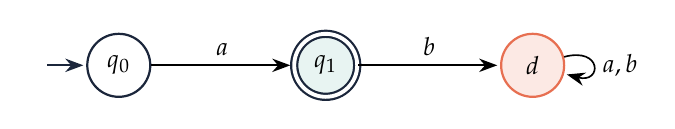
\begin{tikzpicture}[aut,node distance=18mm]
  \node[state,initial] (s) {$q_0$};
  \node[state,accepting] (f) [right=of s] {$q_1$};
  \node[state,dead] (d) [right=of f] {$d$};
  \path (s) edge node {$a$} (f) (f) edge node {$b$} (d) (d) edge[loop right] node {$a,b$} ();
\end{tikzpicture}
\end{center}
\begin{itemize}
\item An arrow from nowhere marks the start state; a double circle (tinted) is an accepting state; a \textcolor{coral}{rose} state is a dead (trap) state.
\item In a transition table, $\to$ marks the start state and $*$ an accepting state.
\item PDA edges are written $a,X/\gamma$: read $a$ (or $\eps$), replace the top $X$ by $\gamma$ (leftmost symbol on top; $\gamma=\eps$ pops). $Z_0$ is the start stack symbol.
\item TM edges are written $X/Y\,D$: read $X$, write $Y$, move $D\in\{L,R\}$. $B$ is the blank.
\end{itemize}
\clearpage
\pagenumbering{arabic}
\topic{01}{Automata concepts and state modelling}

%-------------------------------------------------------------------
\begin{question}{2023--2024 \textbullet\ Q2(c)}{Source N01}{5}
Does the number of accepting DFA states affect the numbers of rows or columns in its transition table? Explain.
\end{question}
\begin{solution}
No. A transition table of a DFA $M=(Q,\Sigma,\delta,q_0,F)$ is simply a tabulation of the total function
$\delta:Q\times\Sigma\to Q$.
\begin{itemize}
\item There is exactly \textbf{one row per state} $q\in Q$, so the number of rows is $|Q|$, regardless of how many of those states are in $F$.
\item There is exactly \textbf{one column per input symbol} $a\in\Sigma$, so the number of columns is $|\Sigma|$.
\end{itemize}
Accepting states are only \emph{marked} (with $*$) in the row label; changing $F$ changes the markings, never the shape.
For example, the parity DFA below has a $2\times 2$ table whether $F=\{E\}$ (even number of 1's) or $F=\{O\}$ (odd) or $F=\{E,O\}$ (everything):
\begin{center}\small
\begin{tabular}{c|cc}\toprule $\delta$ & 0 & 1\\\midrule $\to *E$ & $E$ & $O$\\ $O$ & $O$ & $E$\\\bottomrule\end{tabular}
\end{center}
\ans{Rows $=|Q|$ and columns $=|\Sigma|$; the size of $F$ only affects which rows carry a $*$.}
\end{solution}

%-------------------------------------------------------------------
\begin{question}{2022--2023 \textbullet\ Q1(b)}{Source M49}{12}
An automaton over $\{R,0,1,2\}$ keeps the numerical-symbol sum modulo 3, resets it to 0 on $R$, and accepts remainder 0. A three-state design tracks all remainders. Null Pointer proposes using two states, one for remainder 0 and one for a nonzero remainder. Analyze this claim in detail.
\end{question}
\begin{solution}
\textbf{The correct design.} States $s_0,s_1,s_2$ remember the current sum mod 3; on digit $d$ go from $s_i$ to $s_{(i+d)\bmod 3}$, on $R$ go to $s_0$; accept in $s_0$.
\fig{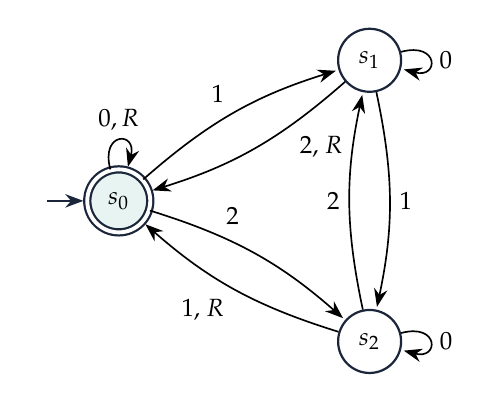
\begin{tikzpicture}[aut,node distance=30mm]
  \node[state,initial,accepting] (0) {$s_0$};
  \node[state] (1) [above right=12mm and 26mm of 0] {$s_1$};
  \node[state] (2) [below right=12mm and 26mm of 0] {$s_2$};
  \path (0) edge[loop above] node {$0,R$} ()
        (0) edge[bend left=12] node {1} (1)
        (0) edge[bend left=12] node[pos=.3] {2} (2)
        (1) edge[bend left=12] node[pos=.3] {2, $R$} (0)
        (1) edge[loop right] node {0} ()
        (1) edge[bend left=12] node {1} (2)
        (2) edge[bend left=12] node {1, $R$} (0)
        (2) edge[loop right] node {0} ()
        (2) edge[bend left=12] node {2} (1);
\end{tikzpicture}}
\textbf{Why two states cannot work.} Suppose a DFA with states $Z$ (remainder 0) and $N$ (``nonzero'') existed. After reading \texttt{1} it is in $N$, and after reading \texttt{2} it is also in $N$. Now append \texttt{1}:
\[
\texttt{1}\cdot\texttt{1}=\texttt{11}:\ 2\not\equiv 0\ (\text{reject}),\qquad
\texttt{2}\cdot\texttt{1}=\texttt{21}:\ 3\equiv 0\ (\text{accept}).
\]
A DFA is deterministic, so from the \emph{same} state $N$ the same suffix \texttt{1} must lead to the same state and the same verdict --- contradiction. The state $N$ has lost the information ``is the remainder 1 or 2?'', which is exactly what is needed to decide the future.

\textbf{Lower bound (distinguishable prefixes).} The prefixes $\eps,\ \texttt{1},\ \texttt{2}$ are pairwise distinguishable:
suffix \texttt{2} separates $\texttt{1}$ (sum 3, accept) from $\eps$ and \texttt{2} (sums 2 and 4, reject); suffix \texttt{1} separates \texttt{2} (sum 3, accept) from $\eps$ (sum 1, reject). If two of them led to the same state, appending the separating suffix would force the same verdict for both, which is impossible. Hence \emph{every} DFA for the language needs at least 3 states.
\ans{The claim is wrong: ``nonzero'' merges remainders 1 and 2, which react differently to future input (e.g.\ suffix \texttt{1}). Three states are necessary and sufficient.}
\end{solution}

%-------------------------------------------------------------------
\begin{question}{2022--2023 \textbullet\ Q2(a)(i--v)}{Source M49--M50}{20 (shared)}
Describe informally the language accepted by each of the five shown automata.
\fig{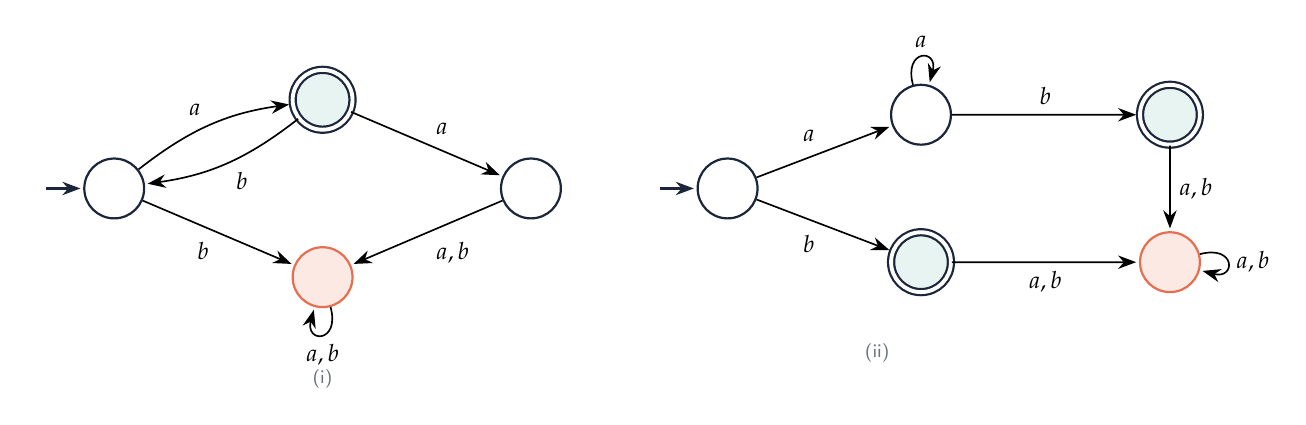
\begin{tikzpicture}[aut,node distance=17mm,scale=.95,transform shape]
 \node[state,initial] (s) {};
 \node[state,accepting] (a) [above right=6mm and 22mm of s] {};
 \node[state] (c) [below right=6mm and 22mm of a] {};
 \node[state,dead] (d) [below right=6mm and 22mm of s] {};
 \path (s) edge[bend left=15] node {$a$} (a) (a) edge[bend left=15] node {$b$} (s)
       (a) edge node {$a$} (c) (c) edge node {$a,b$} (d) (s) edge node[swap] {$b$} (d)
       (d) edge[loop below] node {$a,b$} ();
 \node[below=1mm of d,font=\scriptsize\sffamily,text=slate,yshift=-6mm] {(i)};
 \begin{scope}[xshift=82mm]
 \node[state,initial] (s) {};
 \node[state] (a) [above right=4mm and 20mm of s] {};
 \node[state,accepting] (b) [right=25mm of a] {};
 \node[state,accepting] (c) [below right=4mm and 20mm of s] {};
 \node[state,dead] (d) [right=25mm of c] {};
 \path (s) edge node {$a$} (a) (s) edge node[swap] {$b$} (c) (a) edge[loop above] node {$a$} ()
       (a) edge node {$b$} (b) (b) edge node {$a,b$} (d) (c) edge node[swap] {$a,b$} (d)
       (d) edge[loop right] node {$a,b$} ();
 \node[font=\scriptsize\sffamily,text=slate] at (20mm,-22mm) {(ii)};
 \end{scope}
\end{tikzpicture}}
\fig{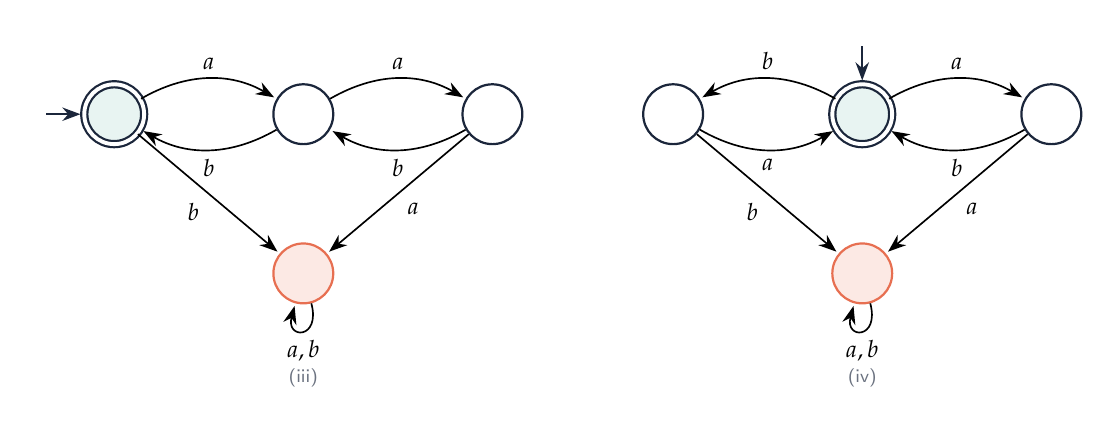
\begin{tikzpicture}[aut,node distance=17mm,scale=.95,transform shape]
 \node[state,initial,accepting] (s) {};
 \node[state] (a) [right=of s] {};
 \node[state] (b) [right=of a] {};
 \node[state,dead] (d) [below=13mm of a] {};
 \path (s) edge[bend left] node {$a$} (a) (a) edge[bend left] node {$b$} (s)
       (a) edge[bend left] node {$a$} (b) (b) edge[bend left] node {$b$} (a)
       (b) edge node {$a$} (d) (s) edge node[swap] {$b$} (d) (d) edge[loop below] node {$a,b$} ();
  \node[font=\scriptsize\sffamily,text=slate] at ($(d)+(0,-14mm)$) {(iii)};
 \begin{scope}[xshift=100mm]
 \node[state,initial above,accepting] (s) {};
 \node[state] (l) [left=of s] {};
 \node[state] (r) [right=of s] {};
 \node[state,dead] (d) [below=13mm of s] {};
 \path (s) edge[bend left] node {$a$} (r) (r) edge[bend left] node {$b$} (s)
       (s) edge[bend right] node[swap] {$b$} (l) (l) edge[bend right] node[swap] {$a$} (s)
       (l) edge node[swap] {$b$} (d) (r) edge node {$a$} (d) (d) edge[loop below] node {$a,b$} ();
 \node[font=\scriptsize\sffamily,text=slate] at ($(d)+(0,-14mm)$) {(iv)};
 \end{scope}
\end{tikzpicture}}
\fig{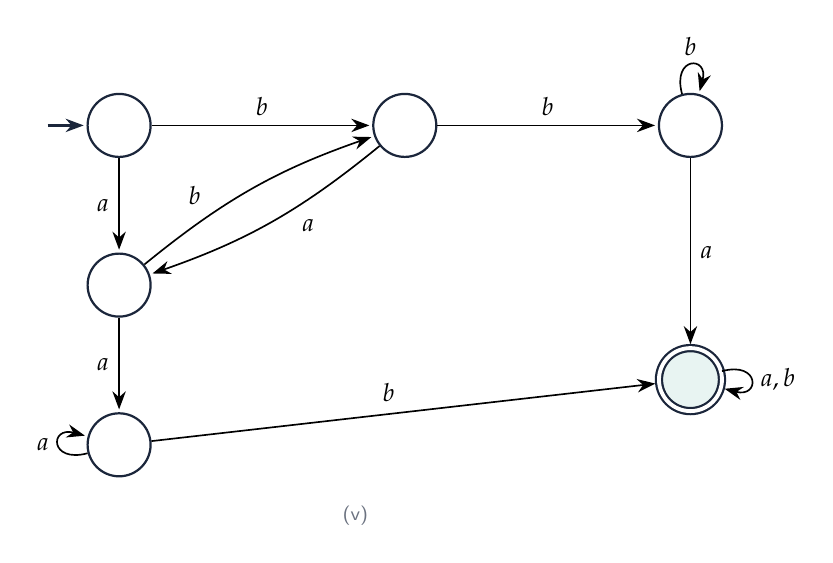
\begin{tikzpicture}[aut,node distance=17mm]
 \node[state,initial] (s) {};
 \node[state] (B) [right=28mm of s] {};
 \node[state] (C) [right=28mm of B] {};
 \node[state] (A) [below=12mm of s] {};
 \node[state] (E) [below=12mm of A] {};
 \node[state,accepting] (F) [below=24mm of C] {};
 \path (s) edge node {$b$} (B) (s) edge node[swap] {$a$} (A)
       (A) edge[bend left=10] node[pos=.3] {$b$} (B) (B) edge[bend left=10] node[pos=.4] {$a$} (A)
       (B) edge node {$b$} (C) (C) edge[loop above] node {$b$} () (C) edge node {$a$} (F)
       (A) edge node[swap] {$a$} (E) (E) edge[loop left] node {$a$} () (E) edge node {$b$} (F)
       (F) edge[loop right] node {$a,b$} ();
 \node[font=\scriptsize\sffamily,text=slate] at ($(E)+(30mm,-9mm)$) {(v)};
\end{tikzpicture}}
\end{question}
\begin{solution}
Trace what each state ``remembers''.
\begin{enumerate}
\item From the start, $a$ leads to the only accepting state; from there $b$ returns to the start and $a$ falls (via an extra state) into the trap. Accepted strings are therefore $a$, $aba$, $ababa,\dots$
\ans{$L_1=(ab)^*a$: strings that alternate $a,b$, starting and ending with $a$.}
\item The upper branch reads $a^+$ then a single $b$ to accept; the lower branch accepts the single symbol $b$. Any further symbol goes to the trap.
\ans{$L_2=a^*b=\{a^nb\mid n\ge 0\}$.}
\item Think of $a$ as ``('' and $b$ as ``)''. The three non-trap states record the current depth $0,1,2$; a third unmatched $a$ (depth 3) or a $b$ at depth 0 goes to the trap, and we accept at depth 0.
\ans{$L_3=(a(ab)^*b)^*$: strings with equally many $a$'s and $b$'s in which every prefix satisfies $0\le \#_a-\#_b\le 2$ (balanced ``parentheses'' of nesting depth at most 2).}
\item From the centre (accepting) state the machine must read either $ab$ or $ba$ to return; $aa$ or $bb$ inside a block leads to the trap.
\ans{$L_4=(ab\cup ba)^*$: even-length strings in which positions $2i-1,2i$ always hold different symbols.}
\item The left column remembers ``last symbol $a$''; the lower-left state remembers ``ends in $aa$'' (it loops on $a$); a $b$ there completes $aab$. Symmetrically the top-right state remembers ``ends in $bb$'' and an $a$ completes $bba$. The final state is a sink.
\ans{$L_5=\{w\mid w \text{ contains } aab \text{ or } bba \text{ as a substring}\}$.}
\end{enumerate}
\end{solution}

%-------------------------------------------------------------------
\begin{question}{2021--2022 \textbullet\ Q1(a)}{Source M44}{4}
Which of the three traditionally central areas of Theory of Computation is applied in a password-protected computer login system? Explain clearly.
\end{question}
\begin{solution}
The three areas are \textbf{automata theory}, \textbf{computability theory} and \textbf{complexity theory}. A login system uses two of them, for two different jobs.
\begin{itemize}
\item \textbf{Automata theory --- checking the password rules.} When a password is chosen, the system checks rules such as ``at least 8 characters, contains a digit, contains an uppercase letter, contains no spaces'' (the ``Password Rules'' example of Lecture~1). This needs only \emph{finite memory}: a DFA that remembers $\min(\text{length},8)$, whether a digit has been seen and whether an uppercase letter has been seen ($9\cdot2\cdot2=36$ states), plus a dead state entered on a space, reads the password once and accepts exactly the valid ones. So the set of valid passwords is a regular language.
\item \textbf{Complexity theory --- keeping stored passwords secure.} The system stores only a hash $h(\text{password})$, where $h$ is a \emph{one-way function}: computing $h$ is easy (polynomial time), so a login attempt is checked quickly, but inverting $h$, or guessing the password by brute force over an exponentially large space, is believed computationally infeasible. Security is an argument about the \emph{difficulty} of computation (the same idea as in cryptography), not about what is computable at all.
\end{itemize}
Computability theory plays no direct role: every task here is decidable; the question is only how much memory or time it needs.
\end{solution}

%-------------------------------------------------------------------
\begin{question}{2021--2022 \textbullet\ Q2(a)}{Source M45}{4}
DFA and NFA recognize the same class of languages. Why is this equivalence both surprising and useful?
\end{question}
\begin{solution}
\textbf{Surprising.} An NFA may branch into many simultaneous computations, use $\eps$-moves and ``guess'' (e.g.\ where a suffix begins). Intuitively this looks strictly more powerful than a single deterministic thread --- for Turing-machine time complexity the analogous question ($\mathrm P$ vs $\mathrm{NP}$) is still open, and for PDAs nondeterminism \emph{does} add power. Yet for finite automata the whole set of currently-active NFA states is itself a finite object (a subset of $Q$), so a DFA can track it: the subset construction removes nondeterminism at the cost of at most $2^{|Q|}$ states.

\textbf{Useful.}
\begin{itemize}
\item \emph{Design}: NFAs are much easier to build and smaller (e.g.\ ``the 3rd symbol from the end is 1'' needs 4 NFA states but 8 DFA states).
\item \emph{Proofs}: closure under union, concatenation and star, and the conversion regex $\to$ automaton, are trivial with NFAs; the equivalence transfers them to DFAs.
\item \emph{Implementation}: DFAs run in one table lookup per symbol, can be complemented by swapping $F$, and tested for equivalence. We design with NFAs and execute with DFAs.
\end{itemize}
\end{solution}

%-------------------------------------------------------------------
\repeated{2}
\begin{question}{2019--2020 \textbullet\ Q2(a)}{Source M40}{5}
Briefly explain the role of a state in a finite automaton.
\end{question}
\begin{question}{2007--2008 \textbullet\ Q2(c)}{Source M04}{5$\tfrac13$}
Describe the most important role played by states in an automaton. Can this role have infinite capacity? Why?
\end{question}
\begin{solution}
\scope{2019--2020 Q2(a) asks only for the role of a state (first paragraph).}
\textbf{Role: states are the machine's only memory.} A finite automaton has no tape or stack; after reading a prefix $x$ it is in one state, and that state must summarise \emph{everything about $x$ that matters for the future}. In short, \key{a state is a compressed summary of the past}: it captures exactly the information needed to determine future behaviour, ignoring irrelevant history. Two prefixes may therefore lead to the same state only if no continuation can ever tell them apart. Example: for ``even number of 1's'' it suffices to remember the parity, so two states $E,O$ suffice; for ``ends in \texttt{01}'' we remember the relevant suffix ($\eps$, \texttt{0}, \texttt{01}).

\textbf{Infinite capacity? No.} A finite automaton has finitely many states $|Q|=k$, so it can remember at most $\lceil\log_2 k\rceil$ bits about an arbitrarily long input. It cannot, for instance, count unboundedly: to recognise $\{0^n1^n\}$ it would have to distinguish $0^1,0^2,0^3,\dots$, i.e.\ infinitely many states. If we allowed infinitely many states the device would no longer be a finite automaton --- in fact it could accept \emph{any} language (one state per prefix, a ``trie''), and it could not be built. Unbounded memory is exactly what PDAs (a stack) and Turing machines (a tape) add.
\ans{The state is a finite memory summarising the relevant past; its capacity is necessarily finite, which is why FAs recognise only regular languages.}
\end{solution}

%-------------------------------------------------------------------
\begin{question}{January 2020 Term \textbullet\ Q2(a)}{Source M36}{7}
State informally the language accepted by the shown DFA.
\fig{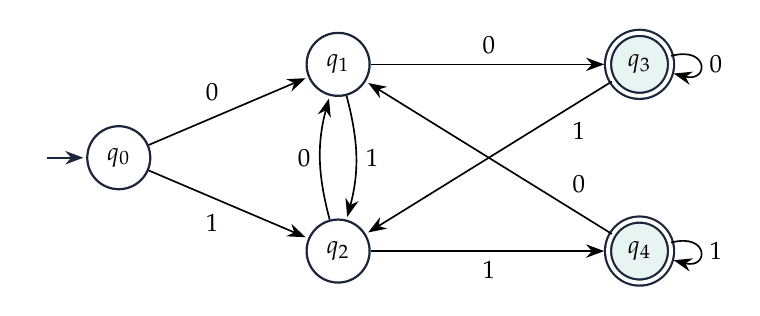
\begin{tikzpicture}[aut,node distance=26mm]
 \node[state,initial] (0) {$q_0$};
 \node[state] (1) [above right=6mm and 22mm of 0] {$q_1$};
 \node[state] (2) [below right=6mm and 22mm of 0] {$q_2$};
 \node[state,accepting] (3) [right=30mm of 1] {$q_3$};
 \node[state,accepting] (4) [right=30mm of 2] {$q_4$};
 \path (0) edge node {0} (1) (0) edge node[swap] {1} (2)
  (1) edge[bend left=15] node {1} (2) (2) edge[bend left=15] node {0} (1)
  (1) edge node {0} (3) (2) edge node[swap] {1} (4)
  (3) edge[loop right] node {0} () (4) edge[loop right] node {1} ()
  (3) edge node[pos=.2] {1} (2) (4) edge node[pos=.2,swap] {0} (1);
\end{tikzpicture}}
\end{question}
\begin{solution}
$q_1$ means ``the last symbol is 0 but the last two are not 00''; $q_3$ means ``the last two symbols are 00''. Symmetrically $q_2$/$q_4$ for 1. Every transition on 0 goes to $q_1$ or $q_3$, every transition on 1 to $q_2$ or $q_4$, and we accept exactly in $q_3,q_4$.
\ans{$L=\{w\in\{0,1\}^*\mid w \text{ ends in } 00 \text{ or } 11\}=(0\cup1)^*(00\cup11)$, i.e.\ the last two symbols are equal.}
\end{solution}

%-------------------------------------------------------------------
\begin{question}{2016--2017 \textbullet\ Q1(a--d)}{Source M28}{(a) 5; (b) 10; (c) 6; (d) 14}
On planet Xustaeter there are red, green, and blue stones. Contact between different colors destroys those two stones and creates two stones of the third color. The planet fails when all stones have one color. Represent each state by (red count, green count, blue count). An $R$-event replaces a green--blue pair by two red stones; define $G$- and $B$-events analogously.
(a) For 3 stones, give a state diagram and classify must-fail, can't-fail, and might-fail states.
(b) Do the same for 4 stones.
(c) Use symmetries in (b) to propose a reduced state-diagram scheme.
(d) Using the scheme from (c), do the same for 6 stones.
\end{question}
\begin{solution}
Events: $R:(r,g,b)\mapsto(r{+}2,g{-}1,b{-}1)$ (needs $g,b\ge1$), and similarly $G,B$. Events happen in any (nondeterministic) order. Classification:
\emph{must-fail} = every sequence of events reaches a monochrome state;
\emph{can't-fail} = no sequence ever does;
\emph{might-fail} = some sequences do and some avoid failure forever.

\textbf{Key invariant.} An $R$-event changes $r-g$ by $+3$, $g-b$ by $0$ and $r-b$ by $+3$; the other events behave alike. Hence the pairwise differences of the counts \emph{mod 3 never change}. A failed state $(n,0,0)$ has two equal counts, so \key{a state whose three counts are pairwise incongruent mod 3 can never fail.}

\sub{(a) Three stones (10 states)}
\fig{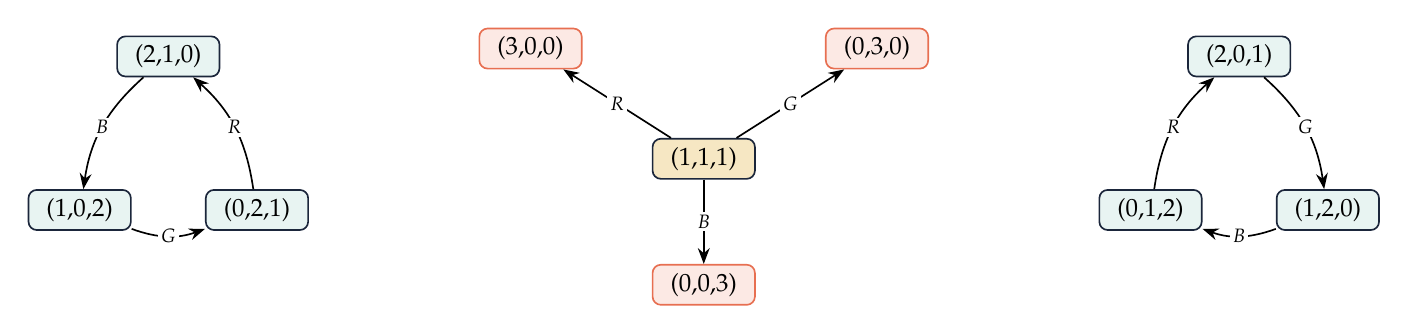
\begin{tikzpicture}[->,>=Stealth,semithick,font=\small,
   st/.style={draw=ink,rounded corners=3pt,fill=white,inner sep=3pt,minimum width=13mm},
   fl/.style={st,fill=rose,draw=coral},mf/.style={st,fill=gold!40}]
 \node[mf] (111) at (0,0) {(1,1,1)};
 \node[fl] (300) at (-2.2,1.4) {(3,0,0)};
 \node[fl] (030) at (2.2,1.4) {(0,3,0)};
 \node[fl] (003) at (0,-1.6) {(0,0,3)};
 \path (111) edge node[lbl] {$R$} (300) (111) edge node[lbl] {$G$} (030) (111) edge node[lbl] {$B$} (003);
 \begin{scope}[xshift=-6.8cm]
  \node[st,fill=mist] (210) at (90:1.3) {(2,1,0)}; \node[st,fill=mist] (102) at (210:1.3) {(1,0,2)}; \node[st,fill=mist] (021) at (330:1.3) {(0,2,1)};
  \path (210) edge[bend right=20] node[lbl] {$B$} (102) (102) edge[bend right=20] node[lbl] {$G$} (021) (021) edge[bend right=20] node[lbl] {$R$} (210);
 \end{scope}
 \begin{scope}[xshift=6.8cm]
  \node[st,fill=mist] (201) at (90:1.3) {(2,0,1)}; \node[st,fill=mist] (120) at (330:1.3) {(1,2,0)}; \node[st,fill=mist] (012) at (210:1.3) {(0,1,2)};
  \path (201) edge[bend left=20] node[lbl] {$G$} (120) (120) edge[bend left=20] node[lbl] {$B$} (012) (012) edge[bend left=20] node[lbl] {$R$} (201);
 \end{scope}
\end{tikzpicture}}
Failed: $(3,0,0),(0,3,0),(0,0,3)$. \key{Must-fail}: $(1,1,1)$ --- each of its three events produces a monochrome state. \key{Can't-fail}: the six permutations of $(2,1,0)$; each has exactly one possible event and they form two 3-cycles (residues $2,1,0$ are distinct). \key{Might-fail}: none.

\sub{(b) Four stones (15 states)}
The diagram splits into three disjoint, identical clusters (one per possible failure colour):
\fig{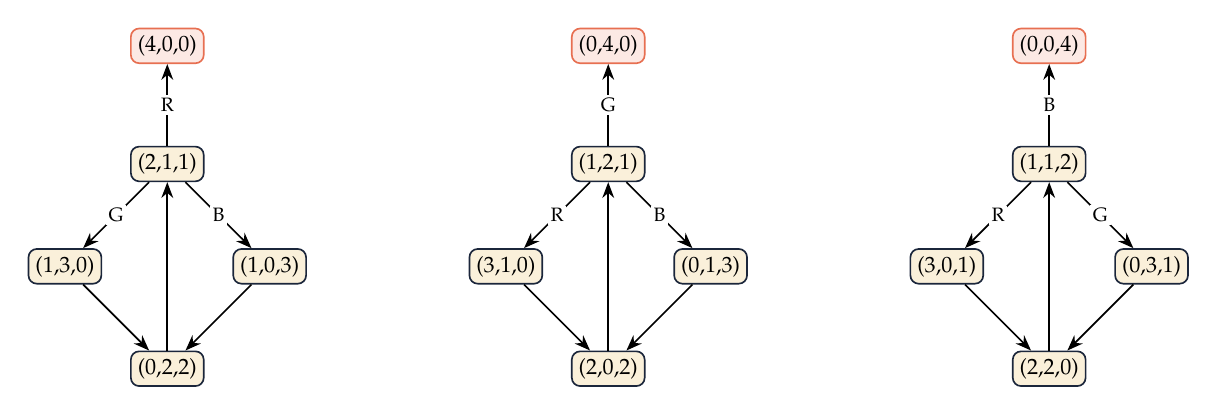
\begin{tikzpicture}[->,>=Stealth,semithick,font=\footnotesize,
   st/.style={draw=ink,rounded corners=3pt,fill=gold!25,inner sep=2.5pt},fl/.style={st,fill=rose,draw=coral}]
 \foreach \x/\h/\m/\n/\l/\f/\e/\ee/\eee in
   {0/{(2,1,1)}/{(1,3,0)}/{(1,0,3)}/{(0,2,2)}/{(4,0,0)}/G/B/R,
    1/{(1,2,1)}/{(3,1,0)}/{(0,1,3)}/{(2,0,2)}/{(0,4,0)}/R/B/G,
    2/{(1,1,2)}/{(3,0,1)}/{(0,3,1)}/{(2,2,0)}/{(0,0,4)}/R/G/B}{
   \node[fl] (f\x) at (\x*5.6,1.5) {\f};
   \node[st] (h\x) at (\x*5.6,0) {\h};
   \node[st] (a\x) at (\x*5.6-1.3,-1.3) {\m};
   \node[st] (b\x) at (\x*5.6+1.3,-1.3) {\n};
   \node[st] (c\x) at (\x*5.6,-2.6) {\l};
   \path (h\x) edge node[lbl] {\eee} (f\x) (h\x) edge node[lbl] {\e} (a\x) (h\x) edge node[lbl] {\ee} (b\x)
         (a\x) edge (c\x) (b\x) edge (c\x) (c\x) edge (h\x);}
\end{tikzpicture}}
(The unlabeled edges are the single possible event of that state, e.g.\ $(1,3,0)\xrightarrow{B}(0,2,2)\xrightarrow{R}(2,1,1)$.)
Failed: $(4,0,0),(0,4,0),(0,0,4)$. Every other state lies on a cycle that avoids failure (e.g.\ $(2,1,1)\to(1,3,0)\to(0,2,2)\to(2,1,1)$) and can also reach the hub's failing edge. Hence \key{all 12 non-failed states are might-fail}; there are no must-fail or can't-fail states. (Consistent with the invariant: $4\equiv1\pmod 3$, so every state has two congruent counts.)

\sub{(c) Reduced scheme}
The rules are symmetric under any permutation of the colours, so a permuted state has the same fate. Represent a state by the \textbf{multiset} of counts $\{x\ge y\ge z\}$ (sorted triple) and draw one node per multiset; an edge $\{x,y,z\}\to\{x',y',z'\}$ exists if some event turns one representative into some representative of the other (optionally labelled by the number of ways). For 4 stones the 15 states collapse to 4 classes:
\fig{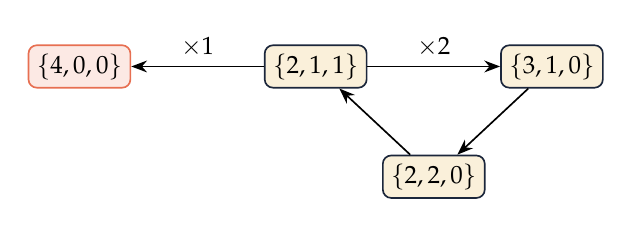
\begin{tikzpicture}[->,>=Stealth,semithick,font=\small,st/.style={draw=ink,rounded corners=3pt,fill=gold!25,inner sep=3pt},fl/.style={st,fill=rose,draw=coral}]
 \node[st] (211) at (0,0) {$\{2,1,1\}$}; \node[st] (310) at (3,0) {$\{3,1,0\}$};
 \node[st] (220) at (1.5,-1.4) {$\{2,2,0\}$}; \node[fl] (400) at (-3,0) {$\{4,0,0\}$};
 \path (211) edge node[above] {$\times2$} (310) (310) edge (220) (220) edge (211) (211) edge node[above] {$\times1$} (400);
\end{tikzpicture}}

\sub{(d) Six stones with the reduced scheme}
The 28 states form 7 classes. Applying the events to a representative of each class:
\[
\{5,1,0\}\to\{4,2,0\}\to\{3,2,1\},\qquad \{3,2,1\}\to\{5,1,0\},\ \{4,2,0\},\ \{3,2,1\};
\]
\[
\{3,3,0\}\to\{2,2,2\}\to\{4,1,1\},\qquad \{4,1,1\}\to\{6,0,0\}\ (\text{fail}),\ \{3,3,0\}.
\]
\fig{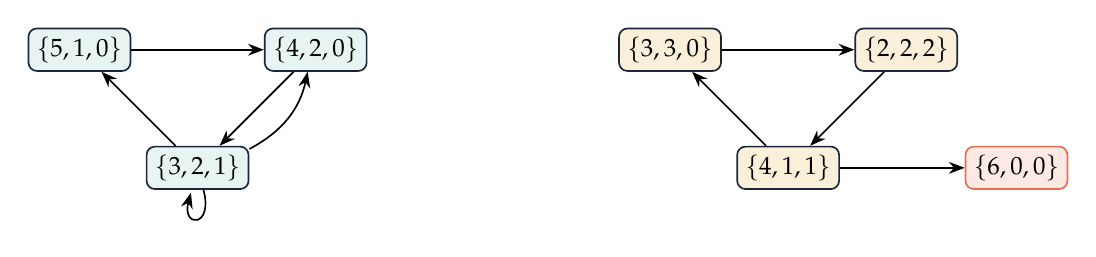
\begin{tikzpicture}[->,>=Stealth,semithick,font=\small,st/.style={draw=ink,rounded corners=3pt,inner sep=3pt},fl/.style={st,fill=rose,draw=coral}]
 \node[st,fill=mist] (510) at (0,0) {$\{5,1,0\}$}; \node[st,fill=mist] (420) at (3,0) {$\{4,2,0\}$}; \node[st,fill=mist] (321) at (1.5,-1.5) {$\{3,2,1\}$};
 \path (510) edge (420) (420) edge (321) (321) edge (510) (321) edge[loop below] ();
 \path (321) edge[bend right=25] (420);
 \begin{scope}[xshift=7.5cm]
 \node[st,fill=gold!25] (330) at (0,0) {$\{3,3,0\}$}; \node[st,fill=gold!25] (222) at (3,0) {$\{2,2,2\}$}; \node[st,fill=gold!25] (411) at (1.5,-1.5) {$\{4,1,1\}$};
 \node[fl] (600) at (4.4,-1.5) {$\{6,0,0\}$};
 \path (330) edge (222) (222) edge (411) (411) edge (330) (411) edge (600);
 \end{scope}
\end{tikzpicture}}
\begin{itemize}
\item \key{Failed}: $\{6,0,0\}$ (3 states).
\item \key{Can't-fail}: $\{5,1,0\},\{4,2,0\},\{3,2,1\}$ --- 18 states. Their counts are $\equiv 0,1,2$ (all different) mod 3, so by the invariant they never fail; indeed the left component never reaches $\{6,0,0\}$.
\item \key{Might-fail}: $\{3,3,0\},\{2,2,2\},\{4,1,1\}$ --- 7 states. The cycle $\{3,3,0\}\to\{2,2,2\}\to\{4,1,1\}\to\{3,3,0\}$ avoids failure, but from $\{4,1,1\}$ the event that merges the two singletons fails.
\item \key{Must-fail}: none (other than already-failed states).
\end{itemize}
\end{solution}

%-------------------------------------------------------------------
\begin{question}{2015--2016 \textbullet\ Q1(a--d)}{Source M24}{(a) 8$\tfrac13$; (b) 4; (c) 4; (d) 4}
For the FSM $F_1$ in the figure:
(a) Formally define an FSM and formally describe $F_1$.
(b) What language does $F_1$ recognize?
(c) Add only $\delta(d,1)=d$ to obtain $F_2$. What language does $F_2$ recognize?
(d) A friend changes $F_1$ without changing its numbers of states and transitions, obtaining $F_3$, and claims $|L(F_3)|=|L(F_1)|+1$. Is that possible? Justify.
\fig{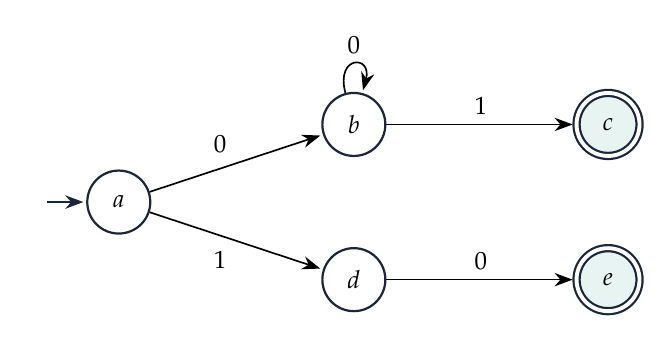
\begin{tikzpicture}[aut,node distance=24mm]
 \node[state,initial] (a) {$a$};
 \node[state] (b) [above right=4mm and 24mm of a] {$b$};
 \node[state] (d) [below right=4mm and 24mm of a] {$d$};
 \node[state,accepting] (c) [right=of b] {$c$};
 \node[state,accepting] (e) [right=of d] {$e$};
 \path (a) edge node {0} (b) (a) edge node[swap] {1} (d) (b) edge[loop above] node {0} ()
       (b) edge node {1} (c) (d) edge node {0} (e);
\end{tikzpicture}}
\end{question}
\begin{solution}
\textbf{(a)} A finite-state machine (DFA) is a 5-tuple $M=(Q,\Sigma,\delta,q_0,F)$: $Q$ a finite set of states, $\Sigma$ a finite input alphabet, $\delta:Q\times\Sigma\to Q$ the transition function, $q_0\in Q$ the start state, $F\subseteq Q$ the accepting states. $M$ accepts $w=w_1\cdots w_n$ iff the run $r_0=q_0,\ r_{i}=\delta(r_{i-1},w_i)$ ends in $r_n\in F$.

The figure omits the moves that lead nowhere; by convention every missing move goes to a non-accepting trap state $t$, which makes $\delta$ total. Formally
$F_1=(\{a,b,c,d,e,t\},\{0,1\},\delta,a,\{c,e\})$ with
\begin{center}\small\begin{tabular}{c|cc}\toprule $\delta$&0&1\\\midrule $\to a$&$b$&$d$\\ $b$&$b$&$c$\\ $*c$&$t$&$t$\\ $d$&$e$&$t$\\ $*e$&$t$&$t$\\ $t$&$t$&$t$\\\bottomrule\end{tabular}\end{center}

\textbf{(b)} Via $b$: one or more 0's then a 1; via $d$: exactly $10$.
\ans{$L(F_1)=0^+1\ \cup\ \{10\}=\{0^n1\mid n\ge1\}\cup\{10\}$ (an infinite language).}

\textbf{(c)} The loop on $d$ allows any number of 1's before the final 0.
\ans{$L(F_2)=0^+1\ \cup\ 1^+0$.}

\textbf{(d)} \emph{Yes, it is possible.} Simply make the start state $a$ accepting. No state or transition is added or removed, and $L(F_3)=L(F_1)\cup\{\eps\}$: exactly one extra string. (Even read purely as cardinalities the claim is consistent: $|L(F_1)|=\aleph_0$ and $\aleph_0+1=\aleph_0$.)
\end{solution}

%-------------------------------------------------------------------
\begin{question}{2015--2016 \textbullet\ Q1(e)}{Source M24}{3}
A regular expression $R_1$ represents exactly five strings. You design an equivalent DFA $D_1$ and correctly implement it in C. The program accepts 1000 distinct random test strings. Your younger brother claims your DFA is wrong. Do you agree? Justify.
\end{question}
\begin{solution}
Yes, the brother is right. If $L(D_1)=L(R_1)$ then $|L(D_1)|=5$, so \emph{at most five} distinct strings can ever be accepted. Since the program (a correct implementation of $D_1$) accepted 1000 distinct strings, at least 995 accepted strings are not in $L(R_1)$; hence $L(D_1)\neq L(R_1)$ --- the DFA design is wrong. (A correct DFA for a finite language of 5 strings must have every path to an accepting state of bounded length, i.e.\ no cycle can lie on a path from the start to an accepting state.)
\end{solution}

%-------------------------------------------------------------------
\repeated{3}
\begin{question}{2012--2013 \textbullet\ Q8(a)}{Source M18}{5}
Give three differences between DFA and NFA, with examples.
\end{question}
\begin{question}{2011--2012 \textbullet\ Q5(a)}{Source M15}{6}
Give three differences between DFA and NFA, with examples.
\end{question}
\begin{question}{2008--2009 \textbullet\ Q5(c)}{Source M07}{5$\tfrac13$}
Define deterministic and nondeterministic finite automata.
\end{question}
\begin{solution}
\scope{2008--2009 Q5(c) asks only for the definitions (first paragraph).}
\textbf{Definitions.} A \key{DFA} is a 5-tuple $M=(Q,\Sigma,\delta,q_0,F)$: $Q$ a finite set of states, $\Sigma$ the input alphabet, $\delta:Q\times\Sigma\to Q$ the transition function, $q_0\in Q$ the start state, $F\subseteq Q$ the accepting states. $M$ accepts $w=w_1w_2\cdots w_n$ ($w_i\in\Sigma$) if there is a sequence of states $r_0,r_1,\dots,r_n$ with $r_0=q_0$, $\delta(r_i,w_{i+1})=r_{i+1}$ for $0\le i\le n-1$, and $r_n\in F$.
An \key{NFA} is a 5-tuple $N=(Q,\Sigma,\delta,q_0,F)$ with the same components except $\delta:Q\times\Sigma_\eps\to\mathcal P(Q)$, where $\Sigma_\eps=\Sigma\cup\{\eps\}$. $N$ accepts $w$ if $w$ can be written as $w=y_1y_2\cdots y_m$ with each $y_i\in\Sigma_\eps$ and there is a sequence of states $r_0,r_1,\dots,r_m$ with $r_0=q_0$, $r_{i+1}\in\delta(r_i,y_{i+1})$ for $0\le i\le m-1$, and $r_m\in F$ --- i.e.\ \emph{at least one} computation branch accepts.

\textbf{Differences.}
\begin{center}\small
\begin{tabularx}{\linewidth}{@{}>{\bfseries}l X X@{}}\toprule
 & DFA & NFA\\\midrule
1. Next move & exactly one next state for each (state, symbol) & zero, one or several next states \\
2. $\eps$-moves & not allowed & allowed (state change without input)\\
3. Acceptance & the unique run ends in $F$ & at least one of the possible runs ends in $F$\\
4. Missing moves & $\delta$ is total & a missing move just kills that branch\\
5. Size/ease & may need up to $2^n$ states & often exponentially smaller, easier to design\\
6. Execution & one table lookup per symbol & must track a set of states (or backtrack)\\\bottomrule
\end{tabularx}\end{center}
\textbf{Example:} $L=\{w\in\{0,1\}^*\mid w \text{ ends in } 01\}$.
\fig{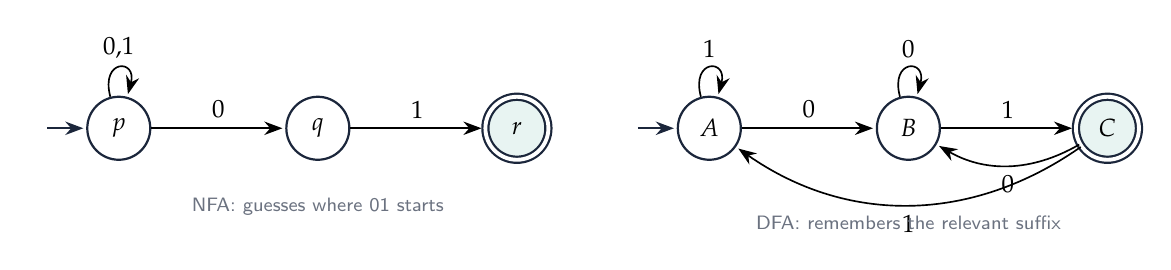
\begin{tikzpicture}[aut,node distance=17mm]
 \node[state,initial] (p) {$p$}; \node[state] (q) [right=of p] {$q$}; \node[state,accepting] (r) [right=of q] {$r$};
 \path (p) edge[loop above] node {0,1} () (p) edge node {0} (q) (q) edge node {1} (r);
 \node[font=\scriptsize\sffamily,text=slate] at ($(q)+(0,-10mm)$) {NFA: guesses where 01 starts};
 \begin{scope}[xshift=75mm]
 \node[state,initial] (A) {$A$}; \node[state] (B) [right=of A] {$B$}; \node[state,accepting] (C) [right=of B] {$C$};
 \path (A) edge[loop above] node {1} () (A) edge node {0} (B) (B) edge[loop above] node {0} ()
       (B) edge node {1} (C) (C) edge[bend left=35] node {1} (A) (C) edge[bend left=30] node {0} (B);
 \node[font=\scriptsize\sffamily,text=slate] at ($(B)+(0,-12mm)$) {DFA: remembers the relevant suffix};
 \end{scope}
\end{tikzpicture}}
In the NFA, $\delta(p,0)=\{p,q\}$ (two choices) and $\delta(q,0)=\emptyset$; the DFA has exactly one arrow per symbol from each state. Both accept the same language.
\end{solution}

%-------------------------------------------------------------------
\begin{question}{2007--2008 \textbullet\ Q1(c)}{Source M04}{5$\tfrac13$}
Explain how set-formers can be used to define a language.
\end{question}
\begin{solution}
A language is a set of strings, $L\subseteq\Sigma^*$, so it can be written with set-builder (``set-former'') notation
\[ L=\{\,w \mid \text{property } P(w) \text{ holds}\,\}\qquad\text{or}\qquad L=\{\,\text{pattern}\mid \text{conditions on its parameters}\,\}. \]
Examples:
\begin{itemize}
\item $\{w\in\{0,1\}^*\mid w \text{ has an equal number of 0's and 1's}\}$ --- a property of the string;
\item $\{0^n1^n\mid n\ge1\}$ --- a pattern with a parameter $n$ and a condition $n\ge1$;
\item $\{0^i1^j\mid 0\le i\le j\}$, $\{w\mid w \text{ is a binary integer that is prime}\}$, $\{ww^R\mid w\in\{a,b\}^*\}$.
\end{itemize}
The notation is precise and compact, can describe infinite languages, and makes membership a logical question (``does $w$ satisfy $P$?''); it is the starting point for designing automata or grammars.
\end{solution}

%-------------------------------------------------------------------
\begin{question}{2006--2007 \textbullet\ Q2(c)}{Source M01}{5$\tfrac13$}
Elaborate, with an example: `One way to think of a nondeterministic computation is as a tree of possibilities.'
\end{question}
\begin{solution}
At each step an NFA may have several choices. Draw the start configuration as the root; each child is a configuration reachable in one move. A path from root to a leaf is one possible computation; the input is \textbf{accepted iff at least one leaf} (after the whole input is read) is an accepting state. Branches with no move simply die. Equivalently the machine ``explores all branches in parallel''; the set of nodes at depth $i$ is the set of states after $i$ symbols --- exactly the DFA state of the subset construction.

\textbf{Example.} NFA for ``ends in 01'' ($p\xrightarrow{0,1}p$, $p\xrightarrow0q$, $q\xrightarrow1r$, $r$ accepting) on input $\texttt{0101}$:
\fig{\begin{forest}pt,for tree={circle,draw=ink,minimum size=6mm,inner sep=0pt,font=\footnotesize,l sep=5mm,s sep=4mm},
 [$p$,[$p$,edge label={node[midway,left,font=\scriptsize]{0}},[$p$,edge label={node[midway,left,font=\scriptsize]{1}},[$p$,edge label={node[midway,left,font=\scriptsize]{0}},[$p$,edge label={node[midway,left,font=\scriptsize]{1}}]][$q$,edge label={node[midway,right,font=\scriptsize]{0}},[$r$,fill=mist,double,edge label={node[midway,right,font=\scriptsize]{1}}]]]]
  [$q$,edge label={node[midway,right,font=\scriptsize]{0}},[$r$,edge label={node[midway,right,font=\scriptsize]{1}},[$\times$,draw=none,font=\small\color{coral},edge label={node[midway,right,font=\scriptsize]{0}}]]]]
\end{forest}}
One leaf at depth 4 is the accepting state $r$, so \texttt{0101} is accepted; the branch through $r$ at depth 2 dies because $r$ has no move on 0.
\end{solution}

\topic{02}{DFA design and numerical languages}

%-------------------------------------------------------------------
\begin{question}{2023--2024 \textbullet\ Q1(b)}{Source N01}{17}
A run is a maximal substring of length at least two consisting of one repeated symbol. For example, $abbbaab$ has a $b$-run of length 3 and an $a$-run of length 2. Design a DFA over $\{a,b\}$ for strings with at most two runs of $a$'s of length exactly three. Give only the state diagram.
\end{question}
\begin{solution}
\textbf{Idea.} Remember two things: $c$ = how many completed $a$-runs of length exactly 3 have been seen ($0,1,2$), and $\ell$ = length of the current block of $a$'s ($0,1,2,3$ or ``$4^+$''). On $a$: $\ell\mapsto\min(\ell+1,4)$. On $b$: the block ends; if $\ell=3$ then $c$ increases (a third one sends us to the dead state $d$), and $\ell\mapsto0$. At the end of input a block of length exactly 3 that is still open also counts, so state $(2{:}3)$ is \emph{rejecting} while every other non-dead state accepts. State $c{:}\ell$ is drawn in row $c$, column $\ell$.
\fig{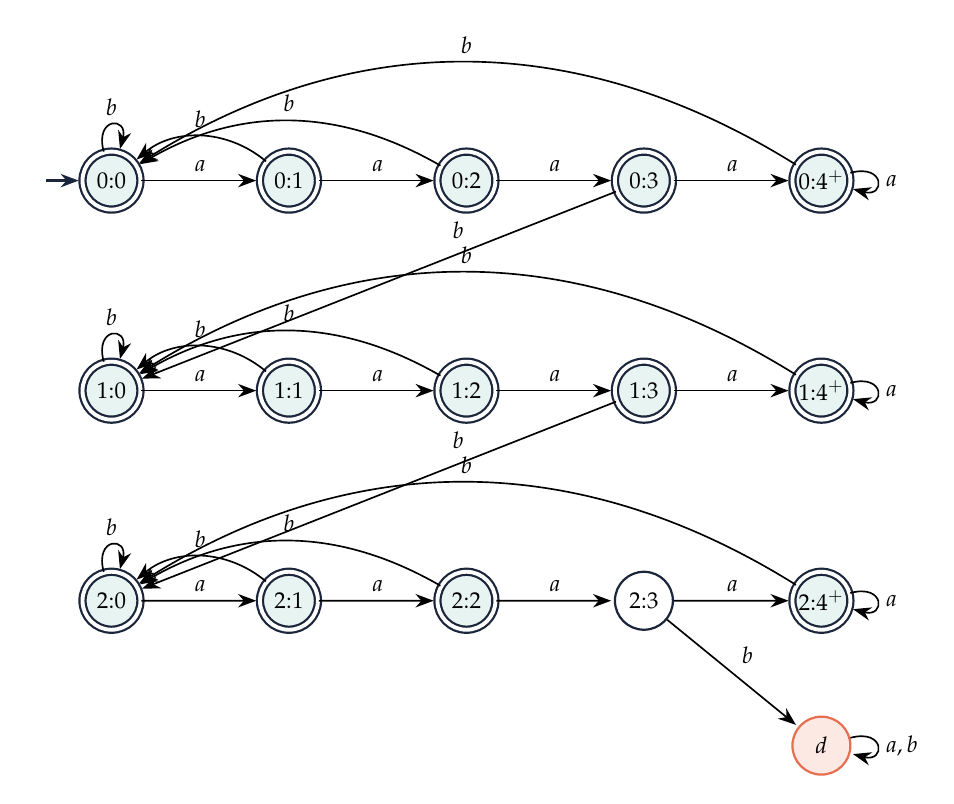
\begin{tikzpicture}[aut,scale=.92,transform shape]
\node[state,initial,accepting] (s00) at (0.00,0.00) {$0{:}0$};
\node[state,accepting] (s01) at (2.45,0.00) {$0{:}1$};
\node[state,accepting] (s02) at (4.90,0.00) {$0{:}2$};
\node[state,accepting] (s03) at (7.35,0.00) {$0{:}3$};
\node[state,accepting] (s04) at (9.80,0.00) {$0{:}4^{+}$};
\node[state,accepting] (s10) at (0.00,-2.90) {$1{:}0$};
\node[state,accepting] (s11) at (2.45,-2.90) {$1{:}1$};
\node[state,accepting] (s12) at (4.90,-2.90) {$1{:}2$};
\node[state,accepting] (s13) at (7.35,-2.90) {$1{:}3$};
\node[state,accepting] (s14) at (9.80,-2.90) {$1{:}4^{+}$};
\node[state,accepting] (s20) at (0.00,-5.80) {$2{:}0$};
\node[state,accepting] (s21) at (2.45,-5.80) {$2{:}1$};
\node[state,accepting] (s22) at (4.90,-5.80) {$2{:}2$};
\node[state] (s23) at (7.35,-5.80) {$2{:}3$};
\node[state,accepting] (s24) at (9.80,-5.80) {$2{:}4^{+}$};
\node[state,dead] (d) at (9.80,-7.80) {$d$};
\path (s00) edge node {$a$} (s01);
\path (s01) edge node {$a$} (s02);
\path (s02) edge node {$a$} (s03);
\path (s03) edge node {$a$} (s04);
\path (s04) edge[loop right] node {$a$} ();
\path (s00) edge[loop above] node {$b$} ();
\path (s01) edge[bend right=40] node[swap] {$b$} (s00);
\path (s02) edge[bend right=30] node[swap] {$b$} (s00);
\path (s04) edge[bend right=32] node[swap] {$b$} (s00);
\path (s03) edge node[pos=.3,swap] {$b$} (s10);
\path (s10) edge node {$a$} (s11);
\path (s11) edge node {$a$} (s12);
\path (s12) edge node {$a$} (s13);
\path (s13) edge node {$a$} (s14);
\path (s14) edge[loop right] node {$a$} ();
\path (s10) edge[loop above] node {$b$} ();
\path (s11) edge[bend right=40] node[swap] {$b$} (s10);
\path (s12) edge[bend right=30] node[swap] {$b$} (s10);
\path (s14) edge[bend right=32] node[swap] {$b$} (s10);
\path (s13) edge node[pos=.3,swap] {$b$} (s20);
\path (s20) edge node {$a$} (s21);
\path (s21) edge node {$a$} (s22);
\path (s22) edge node {$a$} (s23);
\path (s23) edge node {$a$} (s24);
\path (s24) edge[loop right] node {$a$} ();
\path (s20) edge[loop above] node {$b$} ();
\path (s21) edge[bend right=40] node[swap] {$b$} (s20);
\path (s22) edge[bend right=30] node[swap] {$b$} (s20);
\path (s24) edge[bend right=32] node[swap] {$b$} (s20);
\path (s23) edge node {$b$} (d);
\path (d) edge[loop right] node {$a,b$} ();
\end{tikzpicture}}
All 15 states $c{:}\ell$ except $2{:}3$ are accepting. (Brute-force check: this DFA agrees with the definition on all $2^{13}-1$ strings of length $\le 12$.)
\end{solution}

%-------------------------------------------------------------------
\begin{question}{2023--2024 \textbullet\ Q2(b)}{Source N01}{15}
Show that $L=\{awa\mid w\in\{a,b\}^*\}$ is regular by constructing a DFA.
\end{question}
\begin{solution}
$L$ = strings of length $\ge2$ that begin and end with $a$. After the first $a$, state $q_2$ means ``last symbol is $a$'' (accept) and $q_1$ means ``last symbol is $b$ or only the first $a$ was read''.
\fig{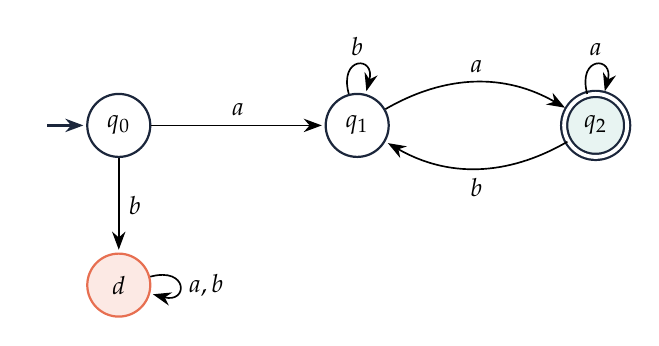
\begin{tikzpicture}[aut,node distance=22mm]
 \node[state,initial] (0) {$q_0$}; \node[state] (1) [right=of 0] {$q_1$}; \node[state,accepting] (2) [right=of 1] {$q_2$};
 \node[state,dead] (d) [below=12mm of 0] {$d$};
 \path (0) edge node {$a$} (1) (1) edge[bend left] node {$a$} (2) (2) edge[bend left] node {$b$} (1)
   (1) edge[loop above] node {$b$} () (2) edge[loop above] node {$a$} () (0) edge node {$b$} (d) (d) edge[loop right] node {$a,b$} ();
\end{tikzpicture}}
Note that the single string $a$ ends in $q_1$ and is rejected, as required ($|awa|\ge2$). Since a DFA recognises $L$, $L$ is regular.
\end{solution}

%-------------------------------------------------------------------
\begin{question}{2022--2023 \textbullet\ Q1(c)}{Source M49}{13}
Construct a DFA for $\{w\in\{a,b\}^*\mid \text{neither } aa \text{ nor } bb \text{ is a substring}\}$. A transition-table representation is required.
\end{question}
\begin{solution}
The strings are exactly the alternating strings. Remember the last symbol.
\begin{center}
\begin{minipage}{.48\linewidth}\centering
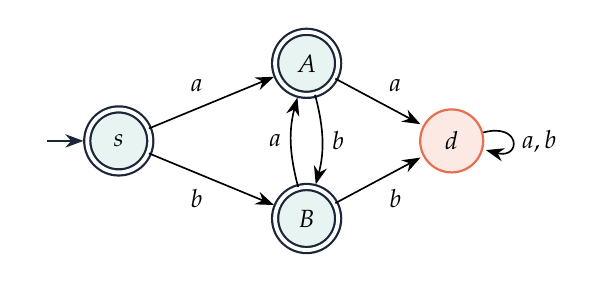
\begin{tikzpicture}[aut,node distance=18mm]
 \node[state,initial,accepting] (s) {$s$}; \node[state,accepting] (A) [above right=4mm and 18mm of s] {$A$};
 \node[state,accepting] (B) [below right=4mm and 18mm of s] {$B$}; \node[state,dead] (d) [right=34mm of s] {$d$};
 \path (s) edge node {$a$} (A) (s) edge node[swap] {$b$} (B) (A) edge[bend left=15] node {$b$} (B) (B) edge[bend left=15] node {$a$} (A)
   (A) edge node {$a$} (d) (B) edge node[swap] {$b$} (d) (d) edge[loop right] node {$a,b$} ();
\end{tikzpicture}\end{minipage}\hfill
\begin{minipage}{.44\linewidth}\centering\small
\begin{tabular}{c|cc}\toprule $\delta$ & $a$ & $b$\\\midrule
$\to *s$ & $A$ & $B$\\ $*A$ & $d$ & $B$\\ $*B$ & $A$ & $d$\\ $d$ & $d$ & $d$\\\bottomrule\end{tabular}\\[2mm]
\footnotesize $s$: nothing read;\ $A/B$: last symbol $a/b$;\ $d$: dead.
\end{minipage}\end{center}
\end{solution}

%-------------------------------------------------------------------
\begin{question}{2022--2023 \textbullet\ Q3(a)}{Source M51}{15}
Construct a DFA accepting binary strings in which no run of 0's has even length $\ge2$. A run is a maximal block of consecutive 0's: 00 has one run of length 2; 000010 has runs of lengths 4 and 1. Reject 0001100, accept 01110001 and 11111. Give a state diagram and explain the design idea.
\end{question}
\begin{solution}
\textbf{Idea.} Every maximal 0-run must have \emph{odd} length. While inside a run we only need its parity; the verdict on a run is given when it ends --- either by a 1 or by the end of the input.
\begin{itemize}
\item $S$: not inside a 0-run (start, or last symbol 1) --- accept.
\item $O$: inside a 0-run of odd length so far --- accept (if the input ends here the run is odd).
\item $E$: inside a 0-run of even length so far --- reject at end; a 1 here closes an even run $\Rightarrow$ dead $d$.
\end{itemize}
\fig{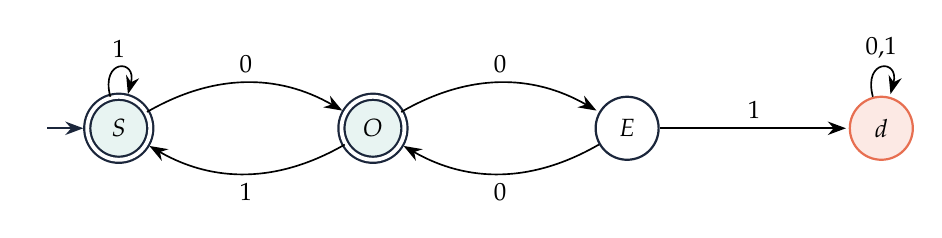
\begin{tikzpicture}[aut,node distance=24mm]
 \node[state,initial,accepting] (S) {$S$}; \node[state,accepting] (O) [right=of S] {$O$}; \node[state] (E) [right=of O] {$E$}; \node[state,dead] (d) [right=of E] {$d$};
 \path (S) edge[loop above] node {1} () (S) edge[bend left] node {0} (O) (O) edge[bend left] node {1} (S)
   (O) edge[bend left] node {0} (E) (E) edge[bend left] node {0} (O) (E) edge node {1} (d) (d) edge[loop above] node {0,1} ();
\end{tikzpicture}}
Checks: $0001100$: runs 000 (odd), 00 (even, ends in $E$) $\Rightarrow$ reject. $01110001$: $S\xrightarrow0O\xrightarrow{111}S\xrightarrow{000}O\xrightarrow1S$ accept. $11111$: stays in $S$, accept.
\end{solution}

%-------------------------------------------------------------------
\begin{question}{2021--2022 \textbullet\ Q1(b)}{Source M44}{10}
Design a DFA with no more than five states over $\{a,b\}$, accepting strings that begin with $a$ and do not contain $aab$. Give only the state diagram.
\end{question}
\begin{solution}
States: $q_0$ start; $A$ = last symbol $a$ (single); $AA$ = ends in $aa$ (a following $b$ would complete $aab$); $B$ = last symbol $b$; $d$ = dead. Five states.
\fig{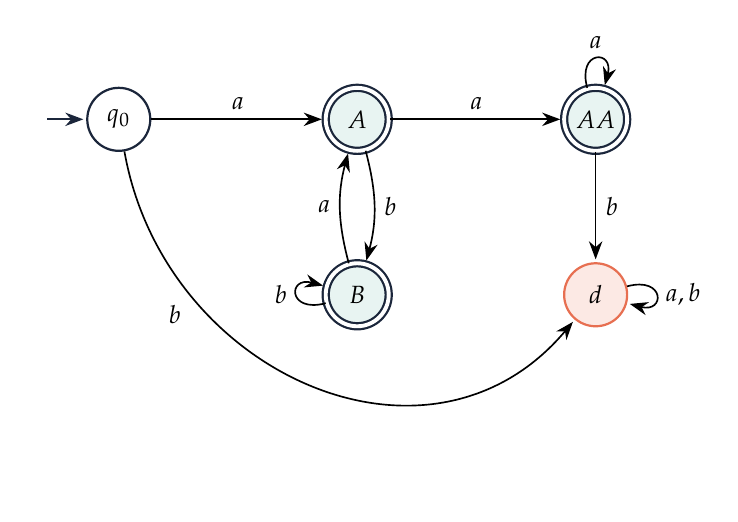
\begin{tikzpicture}[aut,node distance=22mm]
 \node[state,initial] (0) {$q_0$}; \node[state,accepting] (A) [right=of 0] {$A$}; \node[state,accepting] (AA) [right=of A] {$AA$};
 \node[state,accepting] (B) [below=14mm of A] {$B$}; \node[state,dead] (d) [below=14mm of AA] {$d$};
 \path (0) edge node {$a$} (A) (A) edge node {$a$} (AA) (AA) edge[loop above] node {$a$} () (AA) edge node {$b$} (d)
   (A) edge[bend left=15] node {$b$} (B) (B) edge[bend left=15] node {$a$} (A) (B) edge[loop left] node {$b$} ()
   (0) edge[out=-80,in=-130,looseness=1.2] node[swap,pos=.25] {$b$} (d) (d) edge[loop right] node {$a,b$} ();
 \path (0) edge[draw=none] (d);
\end{tikzpicture}}
\end{solution}

%-------------------------------------------------------------------
\begin{question}{2019--2020 \textbullet\ Q1(c)}{Source M40}{15}
Draw a DFA over $\{0,1,2,R\}$ keeping the sum of numerical input symbols, resetting it to 0 on $R$. Accept if the sum is 1 or 2 modulo 5. A state diagram suffices.
\end{question}
\begin{solution}
Only the sum mod 5 matters, so use states $s_0,\dots,s_4$; on digit $d$: $s_i\to s_{(i+d)\bmod5}$; on $R$: $\to s_0$. Accept $s_1,s_2$.
\fig{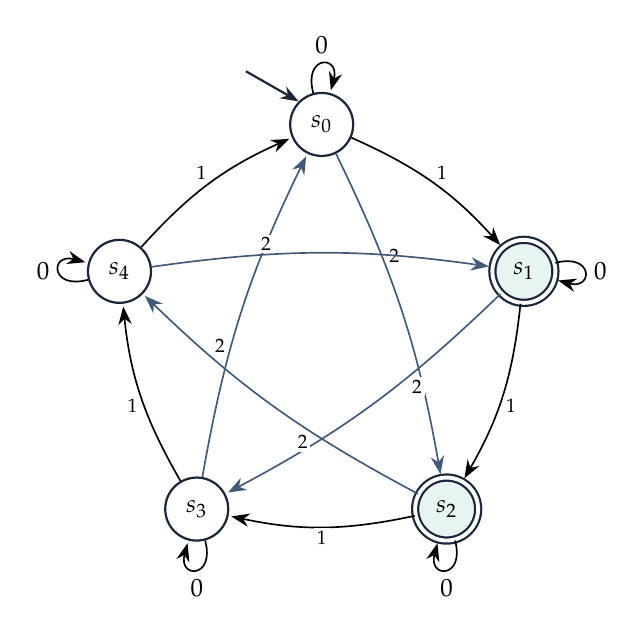
\begin{tikzpicture}[aut]
 \node[state] (s0) at (90:27mm) {$s_0$};
 \node[state,accepting] (s1) at (18:27mm) {$s_1$};
 \node[state,accepting] (s2) at (-54:27mm) {$s_2$};
 \node[state] (s3) at (-126:27mm) {$s_3$};
 \node[state] (s4) at (162:27mm) {$s_4$};
 \draw[ink,thick,<-] (s0.north west) -- ++(-7mm,4mm);
 \path (s0) edge[loop above] node {0} () (s1) edge[loop right] node {0} () (s2) edge[loop below] node {0} () (s3) edge[loop below] node {0} () (s4) edge[loop left] node {0} ();
 \foreach \i/\j in {0/1,1/2,2/3,3/4,4/0}{\path (s\i) edge[bend left=12] node[lbl] {1} (s\j);}
 \foreach \i/\j in {0/2,1/3,2/4,3/0,4/1}{\path (s\i) edge[bend left=8,draw=inksoft] node[lbl,pos=.35] {2} (s\j);}
\end{tikzpicture}}
In addition, \textbf{every} state has an $R$-edge to $s_0$ (omitted from the drawing for clarity; $s_0$ also loops on $R$). Transition table:
\begin{center}\small\begin{tabular}{c|cccc}\toprule & 0&1&2&$R$\\\midrule
$\to s_0$&$s_0$&$s_1$&$s_2$&$s_0$\\ $*s_1$&$s_1$&$s_2$&$s_3$&$s_0$\\ $*s_2$&$s_2$&$s_3$&$s_4$&$s_0$\\ $s_3$&$s_3$&$s_4$&$s_0$&$s_0$\\ $s_4$&$s_4$&$s_0$&$s_1$&$s_0$\\\bottomrule\end{tabular}\end{center}
\end{solution}

%-------------------------------------------------------------------
\begin{question}{2019--2020 \textbullet\ Q2(c)}{Source M40}{15}
Draw a DFA accepting base-3 numbers (digits 0, 1, 2) that are not divisible by 4.
\end{question}
\begin{solution}
Reading digit $d$ after a prefix with value $v$ gives value $3v+d$, so with $r=v\bmod4$: $r\mapsto(3r+d)\bmod4$. The start state is $r=0$ (empty prefix, value 0 --- non-accepting, so $\eps$ is rejected). Accept $r\in\{1,2,3\}$.
\begin{center}
\begin{minipage}{.5\linewidth}\centering
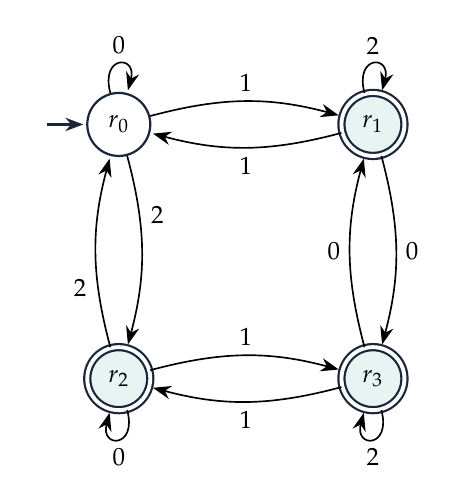
\begin{tikzpicture}[aut,node distance=24mm]
 \node[state,initial] (0) {$r_0$}; \node[state,accepting] (1) [right=of 0] {$r_1$};
 \node[state,accepting] (2) [below=of 0] {$r_2$}; \node[state,accepting] (3) [below=of 1] {$r_3$};
 \path (0) edge[loop above] node {0} () (0) edge[bend left=15] node {1} (1) (0) edge[bend left=15] node[pos=.4] {2} (2)
  (1) edge[bend left=15] node {1} (0) (1) edge[loop above] node {2} () (1) edge[bend left=15] node {0} (3)
  (2) edge[bend left=15] node[pos=.4] {2} (0) (2) edge[loop below] node {0} () (2) edge[bend left=15] node {1} (3)
  (3) edge[bend left=15] node {1} (2) (3) edge[bend left=15] node {0} (1) (3) edge[loop below] node {2} ();
 \path (3) edge[draw=none] (0);
\end{tikzpicture}\end{minipage}\hfill
\begin{minipage}{.42\linewidth}\centering\small
\begin{tabular}{c|ccc}\toprule $r$&0&1&2\\\midrule $\to r_0$&$r_0$&$r_1$&$r_2$\\ $*r_1$&$r_3$&$r_0$&$r_1$\\ $*r_2$&$r_2$&$r_3$&$r_0$\\ $*r_3$&$r_1$&$r_2$&$r_3$\\\bottomrule\end{tabular}\\[1mm]
\footnotesize e.g.\ $12_3=5$: $r_0\xrightarrow1r_1\xrightarrow2r_1$ accept ($5\bmod4=1$).
\end{minipage}\end{center}
\end{solution}

%-------------------------------------------------------------------
\begin{question}{2017--2018 \textbullet\ Q2(b)}{Source M32}{10 + 7 = 17}
Draw DFA state diagrams over $\{0,1\}$ for (i) strings beginning with 1 whose binary value is divisible by 5 (accept 101, 1010, 1111; reject 0, 100, 0101, 111); (ii) strings beginning with 1 whose binary value is a power of 2.
\end{question}
\begin{solution}
\textbf{(i)} Appending bit $b$ maps value $v$ to $2v+b$, so the remainder $r=v\bmod5$ updates as $r\mapsto(2r+b)\bmod5$. A start state $S$ forces the first bit to be 1.
\fig{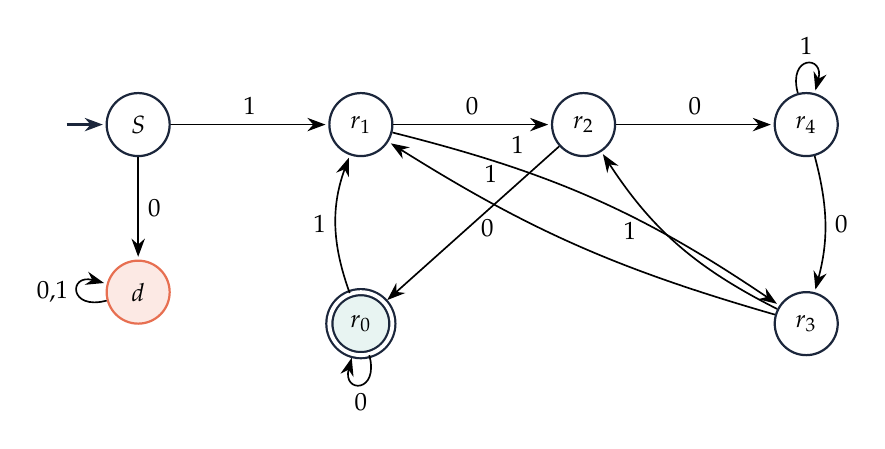
\begin{tikzpicture}[aut,node distance=20mm]
 \node[state,initial] (S) {$S$}; \node[state,dead] (d) [below=13mm of S] {$d$};
 \node[state] (1) [right=of S] {$r_1$}; \node[state] (2) [right=of 1] {$r_2$}; \node[state] (4) [right=of 2] {$r_4$};
 \node[state,accepting] (0) [below=17mm of 1] {$r_0$}; \node[state] (3) [below=17mm of 4] {$r_3$};
 \path (S) edge node {1} (1) (S) edge node {0} (d) (d) edge[loop left] node {0,1} ()
  (1) edge node {0} (2) (1) edge[bend left=10] node[pos=.25] {1} (3) (2) edge node {0} (4) (2) edge node[pos=.3,swap] {1} (0)
  (4) edge[loop above] node {1} () (4) edge[bend left=15] node {0} (3) (3) edge[bend left=15] node[pos=.7] {1} (2)
  (3) edge[bend left=8] node[pos=.7] {0} (1) (0) edge[loop below] node {0} () (0) edge[bend left=20] node {1} (1);
\end{tikzpicture}}
\begin{center}\small\begin{tabular}{c|cc}\toprule&0&1\\\midrule $\to S$&$d$&$r_1$\\ $*r_0$&$r_0$&$r_1$\\ $r_1$&$r_2$&$r_3$\\ $r_2$&$r_4$&$r_0$\\ $r_3$&$r_1$&$r_2$\\ $r_4$&$r_3$&$r_4$\\\bottomrule\end{tabular}\end{center}
Checks: $1111$: $r_1\to r_3\to r_2\to r_0$ (15) accept; $111$: $r_1\to r_3\to r_2$ (7) reject; $0101$: $S\xrightarrow0d$ reject.

\textbf{(ii)} Powers of 2 starting with 1 are exactly $10^*$.
\fig{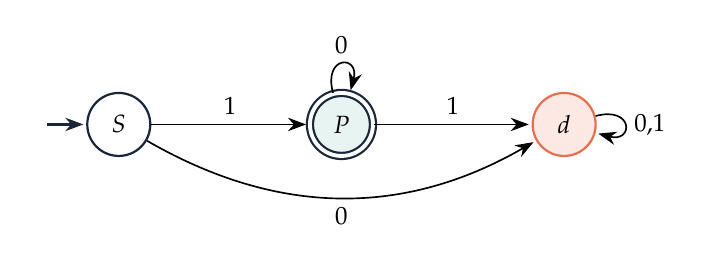
\begin{tikzpicture}[aut,node distance=20mm]
 \node[state,initial] (S) {$S$}; \node[state,accepting] (P) [right=of S] {$P$}; \node[state,dead] (d) [right=of P] {$d$};
 \path (S) edge node {1} (P) (P) edge[loop above] node {0} () (P) edge node {1} (d) (S) edge[bend right=30] node[swap] {0} (d) (d) edge[loop right] node {0,1} ();
\end{tikzpicture}}
\end{solution}

%-------------------------------------------------------------------
\begin{question}{2016--2017 \textbullet\ Q2(a)}{Source M28}{17}
Draw a DFA $D_1$ over $\{a,b,1,2\}$ accepting strings whose number of $a$'s is divisible by 3 and whose sum of digits is even. Accepted examples: $\eps$, $aab12a1$, $aab1bbaaba2a1$, $aaba$, $121$. Rejected: $aaab12a1$, $aab11bbaaba2a1$, $aaaba$, $1121$.
\end{question}
\begin{solution}
Track $(\#_a \bmod 3,\ \text{digit-sum parity})$: six states $(i,p)$. $a$ increments $i$; digit 1 flips $p$; digit 2 and $b$ change nothing. Accept only $(0,E)$.
\fig{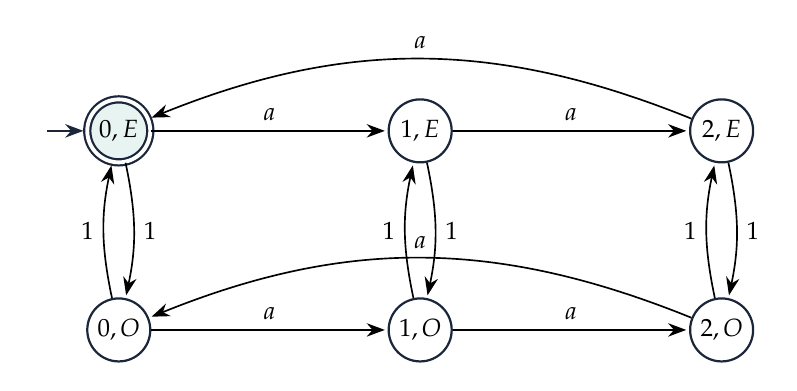
\begin{tikzpicture}[aut,node distance=30mm]
 \node[state,initial,accepting] (0E) {$0,E$}; \node[state] (1E) [right=of 0E] {$1,E$}; \node[state] (2E) [right=of 1E] {$2,E$};
 \node[state] (0O) [below=17mm of 0E] {$0,O$}; \node[state] (1O) [right=of 0O] {$1,O$}; \node[state] (2O) [right=of 1O] {$2,O$};
 \foreach \p in {E,O}{\path (0\p) edge node {$a$} (1\p) (1\p) edge node {$a$} (2\p) (2\p) edge[bend right=22] node[swap] {$a$} (0\p);}
 \foreach \i in {0,1,2}{\path (\i E) edge[bend left=12] node {1} (\i O) (\i O) edge[bend left=12] node {1} (\i E);}
\end{tikzpicture}}
In addition every state has a self-loop on $b$ and on $2$ (not drawn). Check $aab12a1$: $a$'s $=3$, digits $1+2+1=4$ even $\Rightarrow(0,E)$ accept; $1121$: sum 5 odd $\Rightarrow(0,O)$ reject.
\end{solution}

%-------------------------------------------------------------------
\begin{question}{2015--2016 \textbullet\ Q2(a)}{Source M25}{8$\tfrac13$}
Design a DFA accepting binary numbers NOT divisible by 3. It rejects 1111 (15) and accepts 111 (7). Discuss the intuition and explain how it works; a diagram alone is insufficient.
\end{question}
\begin{solution}
\textbf{Intuition.} We cannot store the whole number, but we do not need to: reading the bits left to right, appending a bit $b$ to a prefix of value $v$ produces $2v+b$. Divisibility by 3 depends only on $v\bmod 3$, and
\[ (2v+b)\bmod3=(2\,(v\bmod3)+b)\bmod3 .\]
So three states $r_0,r_1,r_2$ ($r_i$: the prefix read so far has remainder $i$ modulo 3) are enough, with $\delta(r_i,b)=r_{(2i+b)\bmod 3}$:
\begin{center}\small\begin{tabular}{c|cc}\toprule $r$ & 0 & 1\\\midrule $\to r_0$&$r_0$&$r_1$\\ $*r_1$&$r_2$&$r_0$\\ $*r_2$&$r_1$&$r_2$\\\bottomrule\end{tabular}\end{center}
\fig{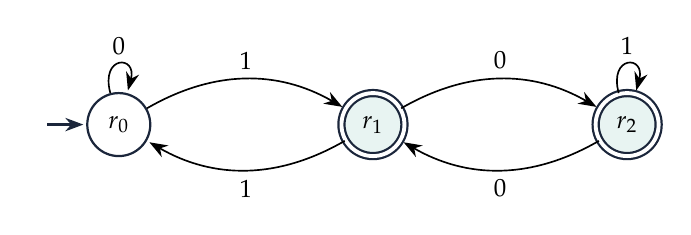
\begin{tikzpicture}[aut,node distance=24mm]
 \node[state,initial] (0) {$r_0$}; \node[state,accepting] (1) [right=of 0] {$r_1$}; \node[state,accepting] (2) [right=of 1] {$r_2$};
 \path (0) edge[loop above] node {0} () (0) edge[bend left] node {1} (1) (1) edge[bend left] node {1} (0)
   (1) edge[bend left] node {0} (2) (2) edge[bend left] node {0} (1) (2) edge[loop above] node {1} ();
\end{tikzpicture}}
The number is \emph{not} divisible by 3 exactly when the remainder is 1 or 2, so $F=\{r_1,r_2\}$. The start state $r_0$ (empty prefix, value 0) is non-accepting, so $\eps$ is rejected as well.

\textbf{How it works on the examples:} $1111$: $r_0\xrightarrow1r_1\xrightarrow1r_0\xrightarrow1r_1\xrightarrow1r_0$ --- remainder 0 ($15=3\cdot5$), $r_0\notin F$, rejected. $111$: $r_0\xrightarrow1 r_1\xrightarrow1 r_0\xrightarrow1 r_1$ --- remainder 1 ($7=3\cdot2+1$), $r_1\in F$, accepted.
\end{solution}

%-------------------------------------------------------------------
\begin{question}{2015--2016 \textbullet\ Q3(a)}{Source M25 \textbullet\ DFA part}{part of 18}
Compute a DFA for each binary language:
(i) begins with 1 and ends with 0;
(ii) length at least 3 and third symbol 0;
(iii) an even number of 0's or exactly two 1's;
(iv) every string except 11 and 111;
(v) at least two 0's and at most one 1.
\end{question}
\begin{solution}
\sub{(i)\quad begins with 1 and ends with 0}
\fig{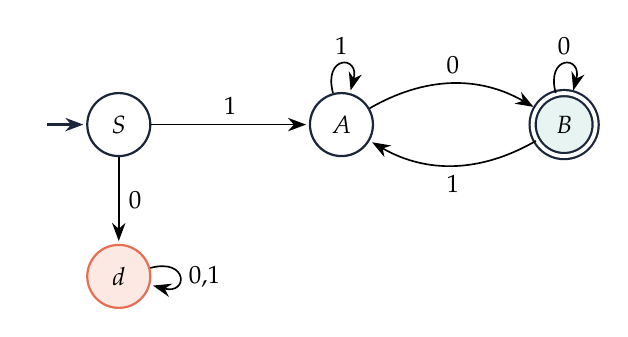
\begin{tikzpicture}[aut,node distance=20mm]
 \node[state,initial] (S) {$S$}; \node[state] (A) [right=of S] {$A$}; \node[state,accepting] (B) [right=of A] {$B$}; \node[state,dead] (d) [below=11mm of S] {$d$};
 \path (S) edge node {1} (A) (A) edge[loop above] node {1} () (A) edge[bend left] node {0} (B) (B) edge[bend left] node {1} (A) (B) edge[loop above] node {0} ()
  (S) edge node {0} (d) (d) edge[loop right] node {0,1} ();
\end{tikzpicture}}
\sub{(ii)\quad length at least 3, third symbol 0}
\fig{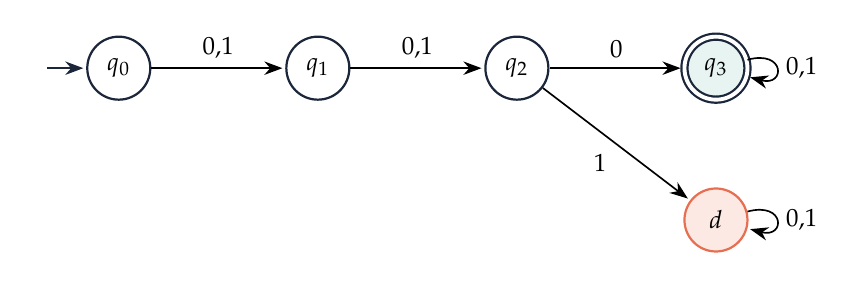
\begin{tikzpicture}[aut,node distance=17mm]
 \node[state,initial] (0) {$q_0$}; \node[state] (1) [right=of 0] {$q_1$}; \node[state] (2) [right=of 1] {$q_2$}; \node[state,accepting] (3) [right=of 2] {$q_3$}; \node[state,dead] (d) [below=11mm of 3] {$d$};
 \path (0) edge node {0,1} (1) (1) edge node {0,1} (2) (2) edge node {0} (3) (3) edge[loop right] node {0,1} () (2) edge node[swap] {1} (d) (d) edge[loop right] node {0,1} ();
\end{tikzpicture}}
\sub{(iii)\quad even number of 0's or exactly two 1's}
Product of ``parity of 0's'' ($E/O$) and ``number of 1's'' ($0,1,2,3^+$); accept when parity is $E$ or count is 2. A 0 moves vertically, a 1 moves right.
\fig{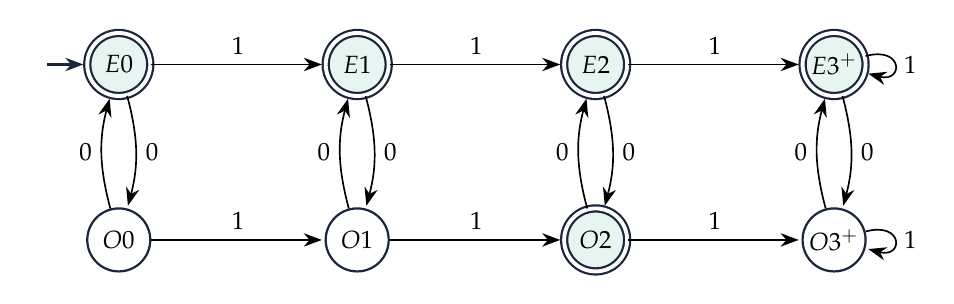
\begin{tikzpicture}[aut,node distance=22mm]
 \node[state,initial,accepting] (E0) {$E0$}; \node[state,accepting] (E1) [right=of E0] {$E1$}; \node[state,accepting] (E2) [right=of E1] {$E2$}; \node[state,accepting] (E3) [right=of E2] {$E3^+$};
 \node[state] (O0) [below=14mm of E0] {$O0$}; \node[state] (O1) [right=of O0] {$O1$}; \node[state,accepting] (O2) [right=of O1] {$O2$}; \node[state] (O3) [right=of O2] {$O3^+$};
 \foreach \p in {E,O}{\path (\p0) edge node {1} (\p1) (\p1) edge node {1} (\p2) (\p2) edge node {1} (\p3) (\p3) edge[loop right] node {1} ();}
 \foreach \i in {0,1,2,3}{\path (E\i) edge[bend left=15] node {0} (O\i) (O\i) edge[bend left=15] node {0} (E\i);}
\end{tikzpicture}}
\sub{(iv)\quad every string except 11 and 111}
Track the prefix while it is still a candidate for $11$ or $111$; any 0 (or a 4th symbol) escapes to an accepting sink $X$.
\fig{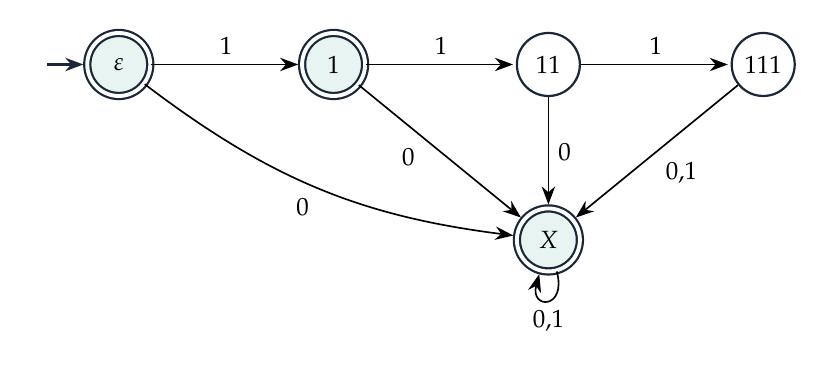
\begin{tikzpicture}[aut,node distance=19mm]
 \node[state,initial,accepting] (e) {$\eps$}; \node[state,accepting] (1) [right=of e] {$1$}; \node[state] (11) [right=of 1] {$11$}; \node[state] (111) [right=of 11] {$111$};
 \node[state,accepting] (X) [below=14mm of 11] {$X$};
 \path (e) edge node {1} (1) (1) edge node {1} (11) (11) edge node {1} (111) (e) edge[bend right=15] node[swap] {0} (X) (1) edge node[swap,pos=.4] {0} (X)
  (11) edge node {0} (X) (111) edge node {0,1} (X) (X) edge[loop below] node {0,1} ();
\end{tikzpicture}}
\sub{(v)\quad at least two 0's and at most one 1}
States $(z,o)$ with $z=\min(\#_0,2)$, $o=\#_1\in\{0,1\}$; a second 1 kills.
\fig{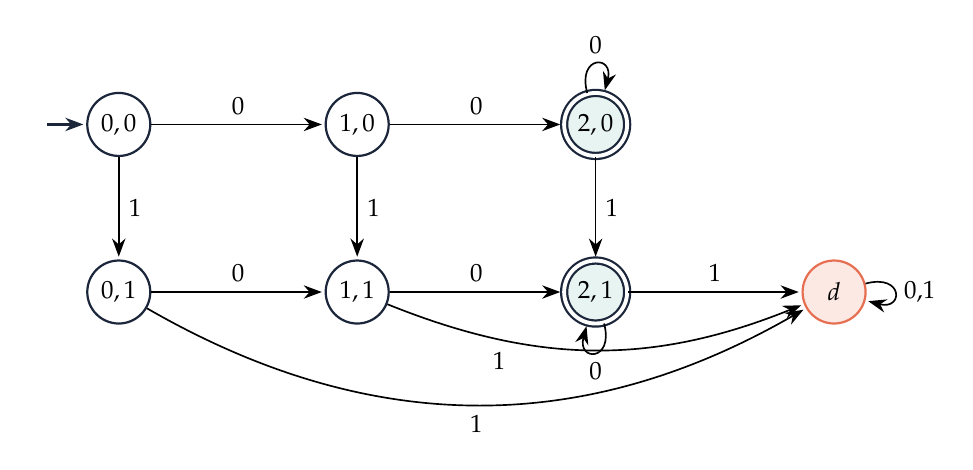
\begin{tikzpicture}[aut,node distance=22mm]
 \node[state,initial] (00) {$0,0$}; \node[state] (10) [right=of 00] {$1,0$}; \node[state,accepting] (20) [right=of 10] {$2,0$};
 \node[state] (01) [below=13mm of 00] {$0,1$}; \node[state] (11) [right=of 01] {$1,1$}; \node[state,accepting] (21) [right=of 11] {$2,1$};
 \node[state,dead] (d) [right=of 21] {$d$};
 \path (00) edge node {0} (10) (10) edge node {0} (20) (20) edge[loop above] node {0} () (01) edge node {0} (11) (11) edge node {0} (21) (21) edge[loop below] node {0} ()
  (00) edge node {1} (01) (10) edge node {1} (11) (20) edge node {1} (21) (21) edge node {1} (d) (d) edge[loop right] node {0,1} ();
 \path (01) edge[bend right=30] node[swap] {1} (d) (11) edge[bend right=22] node[swap,pos=.3] {1} (d);
\end{tikzpicture}}
(All five DFAs were cross-checked by enumeration on all strings up to length 10. The regular expressions asked for in the same question are in the next block.)
\end{solution}

%-------------------------------------------------------------------
\begin{question}{2014--2015 \textbullet\ Q1(a)}{Source M22}{10}
Design a DFA over $\{0,1,2,3,R\}$. Accept exactly strings whose sum of numerical symbols is a multiple of 3, resetting the sum to 0 whenever $R$ occurs. A diagrammatic description suffices.
\end{question}
\begin{solution}
Keep the sum mod 3. Digits 0 and 3 do not change the remainder; 1 adds 1; 2 adds 2; $R$ returns to $s_0$.
\fig{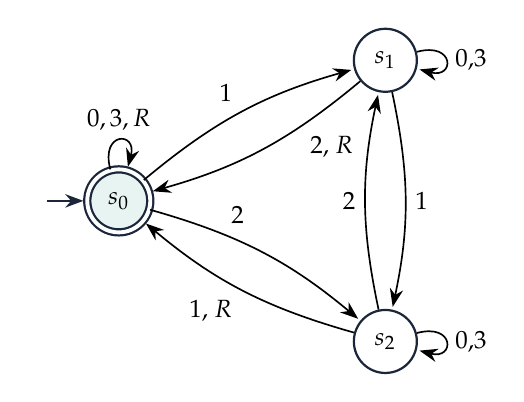
\begin{tikzpicture}[aut,node distance=32mm]
 \node[state,initial,accepting] (0) {$s_0$};
 \node[state] (1) [above right=12mm and 28mm of 0] {$s_1$};
 \node[state] (2) [below right=12mm and 28mm of 0] {$s_2$};
 \path (0) edge[loop above] node {$0,3,R$} ()
       (0) edge[bend left=12] node {1} (1) (0) edge[bend left=12] node[pos=.3] {2} (2)
       (1) edge[bend left=12] node[pos=.3] {2, $R$} (0) (1) edge[loop right] node {0,3} () (1) edge[bend left=12] node {1} (2)
       (2) edge[bend left=12] node {1, $R$} (0) (2) edge[loop right] node {0,3} () (2) edge[bend left=12] node {2} (1);
\end{tikzpicture}}
\end{solution}

\begin{question}{2014--2015 \textbullet\ Q1(b)}{Source M22}{13$\tfrac13$}
Change the alphabet in 1(a) to $\{0,1,2,R\}$ and use states to remember actual sums. Show diagrammatically how to construct this DFA. What is its problem? Explain clearly.
\end{question}
\begin{solution}
Use one state $\Sigma_k$ for each possible actual sum $k$: digit $d$ goes from $\Sigma_k$ to $\Sigma_{k+d}$, $R$ goes back to $\Sigma_0$, and $\Sigma_k$ is accepting iff $3\mid k$.
\fig{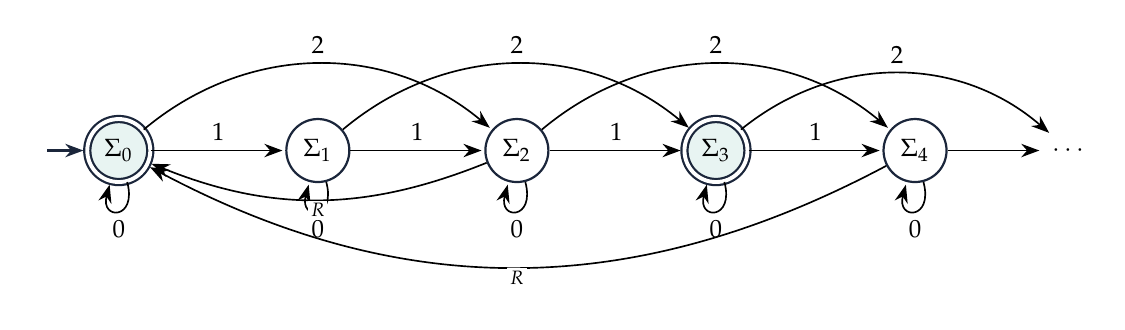
\begin{tikzpicture}[aut,node distance=17mm]
 \node[state,initial,accepting] (0) {$\Sigma_0$}; \node[state] (1) [right=of 0] {$\Sigma_1$}; \node[state] (2) [right=of 1] {$\Sigma_2$};
 \node[state,accepting] (3) [right=of 2] {$\Sigma_3$}; \node[state] (4) [right=of 3] {$\Sigma_4$}; \node (dots) [right=12mm of 4] {$\cdots$};
 \foreach \a/\b in {0/1,1/2,2/3,3/4}{\path (\a) edge node {1} (\b);}
 \foreach \a/\b in {0/2,1/3,2/4}{\path (\a) edge[bend left=40] node {2} (\b);}
 \path (4) edge (dots) (3) edge[bend left=40] node {2} (dots);
 \foreach \a in {0,1,2,3,4}{\path (\a) edge[loop below] node {0} ();}
 \path (4) edge[bend left=28] node[lbl] {$R$} (0) (2) edge[bend left=22] node[lbl] {$R$} (0);
\end{tikzpicture}}
(Every $\Sigma_k$ has an $R$-edge to $\Sigma_0$; only two are drawn.)

\textbf{Problem:} the sum can grow without bound ($111\cdots1$), so this construction needs \emph{infinitely many} states. It is therefore not a finite automaton at all --- it cannot be built or written as a finite table. The fix is to observe that acceptance depends only on $k\bmod 3$, so $\Sigma_k$ and $\Sigma_{k+3}$ behave identically on every future input; merging them gives the 3-state DFA of part (a).
\end{solution}

%-------------------------------------------------------------------
\begin{question}{2014--2015 \textbullet\ Q2(b)}{Source M22}{13$\tfrac13$}
Design a DFA accepting exactly binary-number strings divisible by 4. Explain how it works.
\end{question}
\begin{solution}
Every bit except the last two has place value $2^k$ with $k\ge2$, a multiple of 4. Hence the value modulo 4 is just the value of the last two bits, and a binary number is divisible by $4=2^2$ iff it ends in 00 or is the single digit $0$. So the DFA only has to remember the relevant suffix of what it has read. DFA (states = relevant suffix):
\fig{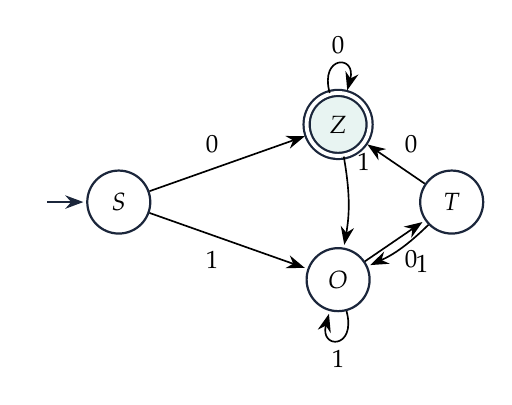
\begin{tikzpicture}[aut,node distance=24mm]
 \node[state,initial] (S) {$S$}; \node[state,accepting] (A) [above right=4mm and 22mm of S] {$Z$};
 \node[state] (B) [below right=4mm and 22mm of S] {$O$}; \node[state] (C) [right=34mm of S] {$T$};
 \path (S) edge node {0} (A) (S) edge node[swap] {1} (B) (A) edge[loop above] node {0} () (A) edge[bend left=10] node[pos=.25] {1} (B)
  (B) edge[loop below] node {1} () (B) edge node[swap] {0} (C) (C) edge node[swap] {0} (A) (C) edge[bend left=10] node[pos=.4] {1} (B);
\end{tikzpicture}}
$Z$: value $\equiv 0\pmod 4$ (ends in 00, or the string is $0$/$00$); $O$: last bit 1 (value odd); $T$: ends in 10 (value $\equiv2$). Reading 0 from $O$ gives $\equiv2$; reading 0 from $T$ gives $\equiv0$; reading 1 always gives an odd number. $S$ is a non-accepting start state so that $\eps$ is not accepted. Example: $1100$ (12): $S\to O\to O\to T\to Z$ accept; $110$ (6): ends in $T$, reject.
\end{solution}

%-------------------------------------------------------------------
\begin{question}{2013--2014 \textbullet\ Q5(c)}{Source M20}{10$\tfrac13$}
Construct a DFA recognizing $\{w\in\{a,b\}^*\mid w=a^pb^q \text{ and } p+q \text{ is even}\}$.
\end{question}
\begin{solution}
$L$ = even-length strings of the form $a^*b^*$. Track phase ($a$-part or $b$-part) and length parity; an $a$ after a $b$ is fatal.
\fig{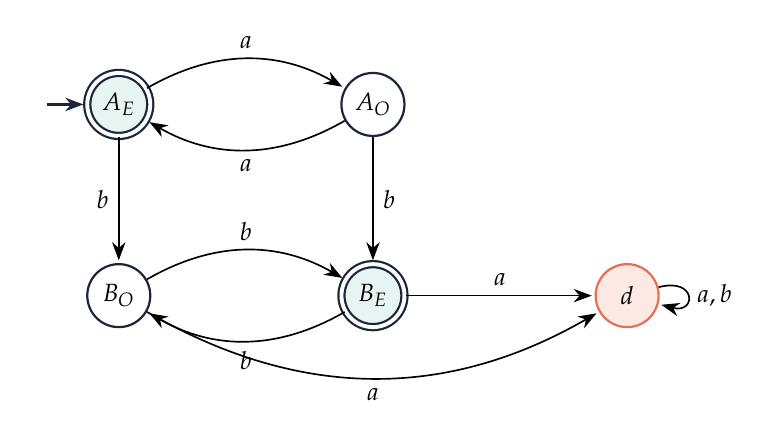
\begin{tikzpicture}[aut,node distance=24mm]
 \node[state,initial,accepting] (A0) {$A_E$}; \node[state] (A1) [right=of A0] {$A_O$};
 \node[state] (B1) [below=16mm of A0] {$B_O$}; \node[state,accepting] (B0) [below=16mm of A1] {$B_E$}; \node[state,dead] (d) [right=of B0] {$d$};
 \path (A0) edge[bend left] node {$a$} (A1) (A1) edge[bend left] node {$a$} (A0) (A0) edge node[swap] {$b$} (B1) (A1) edge node {$b$} (B0)
  (B1) edge[bend left] node {$b$} (B0) (B0) edge[bend left] node {$b$} (B1) (B0) edge node {$a$} (d) (B1) edge[bend right=30] node[swap] {$a$} (d) (d) edge[loop right] node {$a,b$} ();
\end{tikzpicture}}
$A_E/A_O$: only $a$'s so far, even/odd length; $B_E/B_O$: in the $b$-part, even/odd total length.
\end{solution}

%-------------------------------------------------------------------
\begin{question}{2012--2013 \textbullet\ Q7(c)}{Source M18}{8}
Design a DFA for binary strings whose decimal values are multiples of five.
\end{question}
\begin{solution}
Same idea as for divisibility by 3 (2015--2016 Q2(a), 2008--2009 Q6(a)): remainder $r=v\bmod5$, update $r\mapsto(2r+b)\bmod5$, accept $r_0$. The empty string has no decimal value, so a separate non-accepting start state $q_s$ (no bit read yet) has the moves of $r_0$: $q_s\xrightarrow0r_0$, $q_s\xrightarrow1r_1$.
\fig{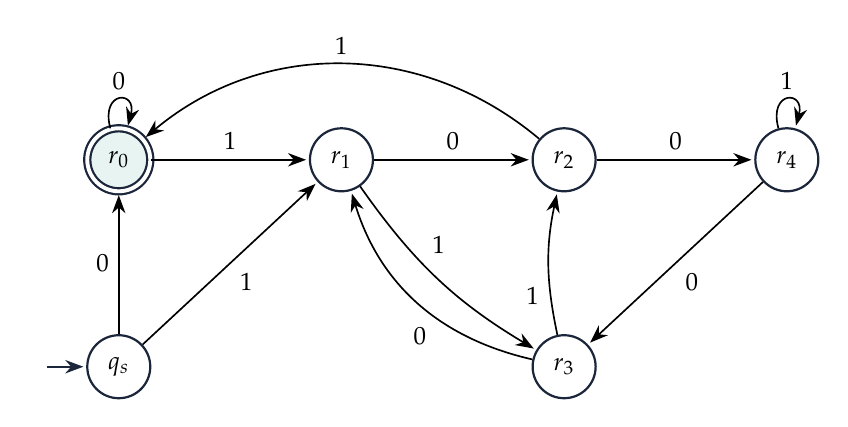
\begin{tikzpicture}[aut,node distance=20mm]
 \node[state,accepting] (0) {$r_0$}; \node[state] (1) [right=of 0] {$r_1$}; \node[state] (2) [right=of 1] {$r_2$}; \node[state] (4) [right=of 2] {$r_4$};
 \node[state] (3) [below=18mm of 2] {$r_3$}; \node[state,initial] (s) [below=18mm of 0] {$q_s$};
 \path (s) edge node {0} (0) (s) edge node[swap] {1} (1)
  (0) edge[loop above] node {0} () (0) edge node {1} (1) (1) edge node {0} (2) (1) edge[bend right=12] node[pos=.4] {1} (3)
  (2) edge node {0} (4) (2) edge[bend right=40] node[swap] {1} (0) (4) edge[loop above] node {1} () (4) edge node {0} (3)
  (3) edge[bend left=30] node[pos=.4] {0} (1) (3) edge[bend left=12] node[pos=.4] {1} (2);
\end{tikzpicture}}
\begin{center}\small\begin{tabular}{c|ccccc}\toprule $r$&0&1&2&3&4\\\midrule on 0&$r_0$&$r_2$&$r_4$&$r_1$&$r_3$\\ on 1&$r_1$&$r_3$&$r_0$&$r_2$&$r_4$\\\bottomrule\end{tabular}\end{center}
Example $1010$ (10): $q_s\to r_1\to r_2\to r_0\to r_0$ accept; $\eps$ stays in $q_s$, rejected.
\end{solution}

%-------------------------------------------------------------------
\begin{question}{2011--2012 \textbullet\ Q5(c)}{Source M15}{5$\tfrac13$}
Give the state diagram of a DFA recognizing $\{w\mid |w|\le5\}$ over $\{0,1\}$.
\end{question}
\begin{solution}
Count the length up to 5; the sixth symbol leads to a dead state.
\fig{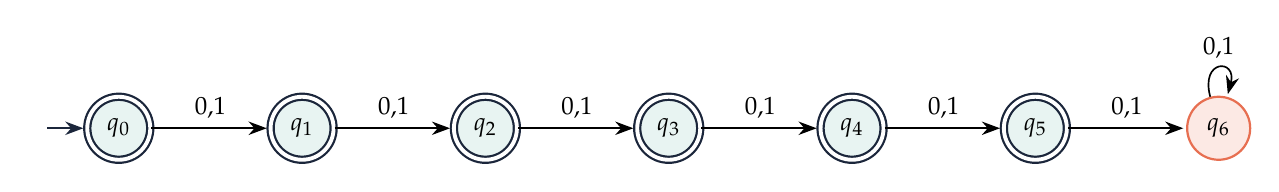
\begin{tikzpicture}[aut,node distance=15mm]
 \node[state,initial,accepting] (0) {$q_0$};
 \foreach \i [count=\j from 0] in {1,...,5}{\node[state,accepting] (\i) [right=of \j] {$q_\i$}; \path (\j) edge node {0,1} (\i);}
 \node[state,dead] (6) [right=of 5] {$q_6$}; \path (5) edge node {0,1} (6) (6) edge[loop above] node {0,1} ();
\end{tikzpicture}}
\end{solution}

%-------------------------------------------------------------------
\begin{question}{2010--2011 \textbullet\ Q2}{Source M11}{10}
Design a DFA for strings over $\{a,b\}$ satisfying $n\bmod3=1$, where $n$ is the number of $a$'s. Give a transition diagram and mathematical representation.
\end{question}
\begin{solution}
\fig{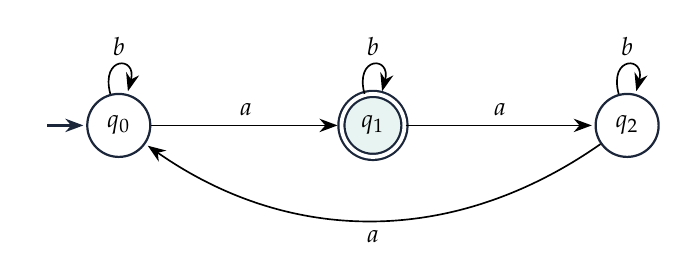
\begin{tikzpicture}[aut,node distance=24mm]
 \node[state,initial] (0) {$q_0$}; \node[state,accepting] (1) [right=of 0] {$q_1$}; \node[state] (2) [right=of 1] {$q_2$};
 \path (0) edge node {$a$} (1) (1) edge node {$a$} (2) (2) edge[bend left=35] node {$a$} (0)
  (0) edge[loop above] node {$b$} () (1) edge[loop above] node {$b$} () (2) edge[loop above] node {$b$} ();
\end{tikzpicture}}
$M=(\{q_0,q_1,q_2\},\{a,b\},\delta,q_0,\{q_1\})$ with $\delta(q_i,a)=q_{(i+1)\bmod3}$ and $\delta(q_i,b)=q_i$. State $q_i$ means $\#_a\equiv i\pmod3$.
\end{solution}

%-------------------------------------------------------------------
\begin{question}{2010--2011 \textbullet\ Q4}{Source M11 \textbullet\ DFA part}{7}
Design a DFA for binary strings not containing substring 110.
\end{question}
\begin{solution}
States record the longest suffix that is a prefix of 110: $q_0$ (none), $q_1$ (``1''), $q_2$ (``11''), $d$ (110 seen).
\fig{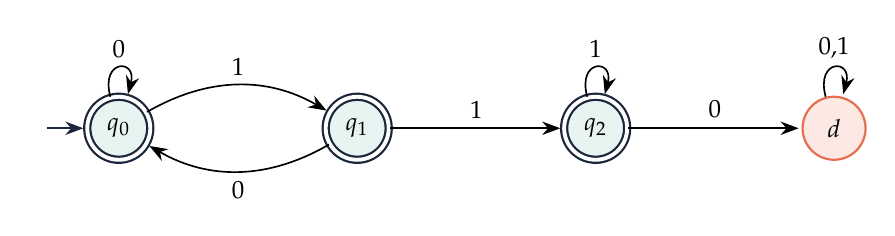
\begin{tikzpicture}[aut,node distance=22mm]
 \node[state,initial,accepting] (0) {$q_0$}; \node[state,accepting] (1) [right=of 0] {$q_1$}; \node[state,accepting] (2) [right=of 1] {$q_2$}; \node[state,dead] (d) [right=of 2] {$d$};
 \path (0) edge[loop above] node {0} () (0) edge[bend left] node {1} (1) (1) edge[bend left] node {0} (0) (1) edge node {1} (2)
  (2) edge[loop above] node {1} () (2) edge node {0} (d) (d) edge[loop above] node {0,1} ();
\end{tikzpicture}}
All three non-dead states accept. (The regular expression asked for in the same question is in the next block.)
\end{solution}

%-------------------------------------------------------------------
\begin{question}{2009--2010 \textbullet\ Q2}{Source M08}{10}
Design a DFA for strings over $\{a,b\}$ that never contain three consecutive occurrences of the character that started the string. Thus $abaab$ and $baaabba$ are accepted; $abaaab$ and $bbbaa$ are rejected. Give a transition diagram.
\end{question}
\begin{solution}
The first symbol selects one of two symmetric sub-machines; each counts the current run of the starting character (1 or 2). $\eps$ is accepted vacuously.
\fig{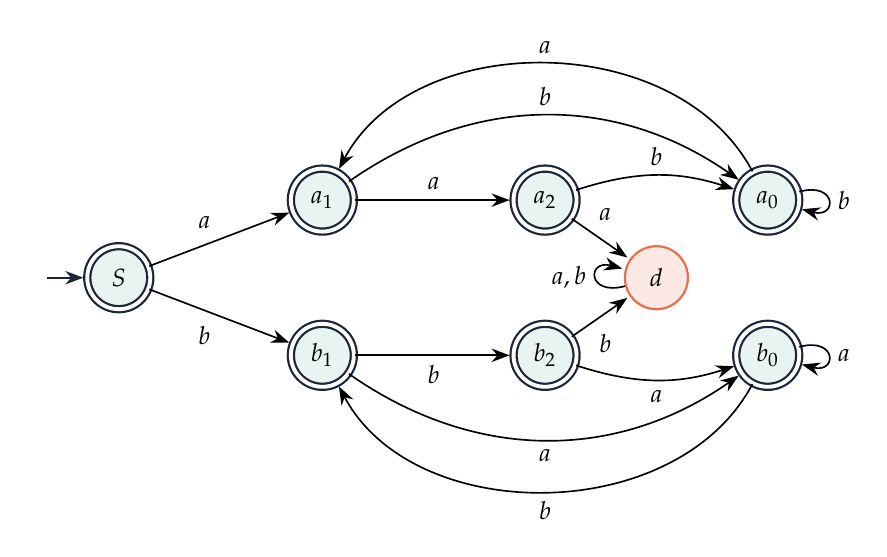
\begin{tikzpicture}[aut,node distance=20mm]
 \node[state,initial,accepting] (S) {$S$};
 \node[state,accepting] (a1) [above right=4mm and 20mm of S] {$a_1$}; \node[state,accepting] (a2) [right=of a1] {$a_2$}; \node[state,accepting] (a0) [right=of a2] {$a_0$};
 \node[state,accepting] (b1) [below right=4mm and 20mm of S] {$b_1$}; \node[state,accepting] (b2) [right=of b1] {$b_2$}; \node[state,accepting] (b0) [right=of b2] {$b_0$};
 \node[state,dead] (d) [right=60mm of S] {$d$};
 \path (S) edge node {$a$} (a1) (S) edge node[swap] {$b$} (b1)
  (a1) edge node {$a$} (a2) (a2) edge node[pos=.3] {$a$} (d) (a1) edge[bend left=35] node {$b$} (a0) (a2) edge[bend left=18] node {$b$} (a0)
  (a0) edge[loop right] node {$b$} () (a0) edge[bend right=62] node[swap] {$a$} (a1)
  (b1) edge node[swap] {$b$} (b2) (b2) edge node[swap,pos=.3] {$b$} (d) (b1) edge[bend right=35] node[swap] {$a$} (b0) (b2) edge[bend right=18] node[swap] {$a$} (b0)
  (b0) edge[loop right] node {$a$} () (b0) edge[bend left=62] node {$b$} (b1) (d) edge[loop left] node {$a,b$} ();
\end{tikzpicture}}
$a_k$ ($k=0,1,2$): the string started with $a$ and currently ends in exactly $k$ consecutive $a$'s; symmetric for $b_k$. Checks: $abaaab$: $S\to a_1\to a_0\to a_1\to a_2\to d$ reject; $baaabba$: $S\to b_1\to b_0\to b_0\to b_0\to b_1\to b_2\to b_0$ accept.
\end{solution}

%-------------------------------------------------------------------
\begin{question}{2008--2009 \textbullet\ Q6(a)}{Source M07}{9}
Design a DFA accepting binary strings whose decimal values are multiples of three.
\end{question}
\begin{solution}
Same remainder states $r_0,r_1,r_2$ and moves $\delta(r_i,b)=r_{(2i+b)\bmod3}$ as in 2015--2016 Q2(a) above, but now the accepting set is $F=\{r_0\}$ (remainder 0). The empty string has no decimal value, so --- as in the slides --- we add a separate non-accepting start state $q_s$ (no bit read yet) whose moves are those of $r_0$; we accept when at least one bit has been read and the remainder is 0.
\fig{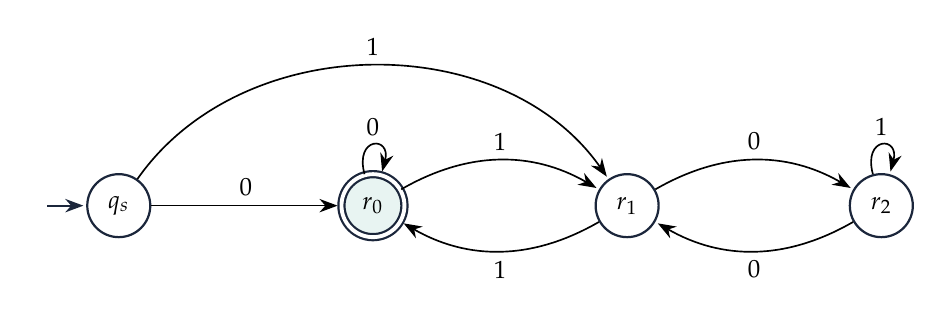
\begin{tikzpicture}[aut,node distance=24mm]
 \node[state,initial] (s) {$q_s$}; \node[state,accepting] (0) [right=of s] {$r_0$}; \node[state] (1) [right=of 0] {$r_1$}; \node[state] (2) [right=of 1] {$r_2$};
 \path (s) edge node {0} (0) (s) edge[bend left=55] node {1} (1)
   (0) edge[loop above] node {0} () (0) edge[bend left] node {1} (1) (1) edge[bend left] node {1} (0)
   (1) edge[bend left] node {0} (2) (2) edge[bend left] node {0} (1) (2) edge[loop above] node {1} ();
\end{tikzpicture}}
$M=(\{q_s,r_0,r_1,r_2\},\{0,1\},\delta,q_s,\{r_0\})$. E.g.\ $1001$ (9): $q_s\xrightarrow1r_1\xrightarrow0r_2\xrightarrow0r_1\xrightarrow1r_0$, accepted; $100$ (4): ends in $r_1$, rejected.
\end{solution}

%-------------------------------------------------------------------
\begin{question}{2007--2008 \textbullet\ Q1(b)}{Source M04}{8}
Design a DFA for strings over $\{a,b\}$ in which every $a$ is followed by at least one $b$. Mention the design steps and give both a transition diagram and a transition table.
\end{question}
\begin{solution}
\textbf{Steps.} (1) Fix the reading: every $a$ must be \emph{immediately} followed by a $b$, i.e.\ $L=(b\cup ab)^*$. (2) Decide what to remember: whether an $a$ is still ``waiting'' for its $b$. (3) States: $q_0$ = nothing pending (accepting), $q_1$ = an $a$ is pending, $d$ = violation (an $a$ was followed by $a$). (4) Add transitions, mark $F=\{q_0\}$.
\begin{center}
\begin{minipage}{.5\linewidth}\centering
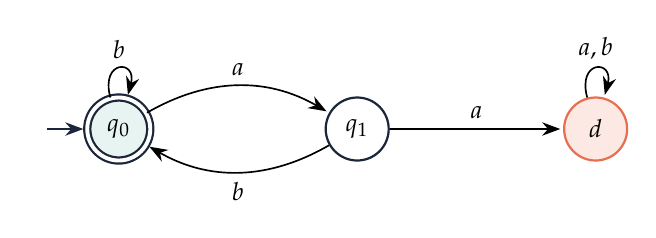
\begin{tikzpicture}[aut,node distance=22mm]
 \node[state,initial,accepting] (0) {$q_0$}; \node[state] (1) [right=of 0] {$q_1$}; \node[state,dead] (d) [right=of 1] {$d$};
 \path (0) edge[loop above] node {$b$} () (0) edge[bend left] node {$a$} (1) (1) edge[bend left] node {$b$} (0) (1) edge node {$a$} (d) (d) edge[loop above] node {$a,b$} ();
\end{tikzpicture}\end{minipage}
\begin{minipage}{.35\linewidth}\centering\small
\begin{tabular}{c|cc}\toprule&$a$&$b$\\\midrule $\to*q_0$&$q_1$&$q_0$\\ $q_1$&$d$&$q_0$\\ $d$&$d$&$d$\\\bottomrule\end{tabular}\end{minipage}\end{center}
(If ``followed'' is read as ``followed somewhere later'', the language is just ``$\eps$ or ends in $b$'' and the same diagram works with the $q_1\xrightarrow a d$ edge replaced by a self-loop on $q_1$.)
\end{solution}

%-------------------------------------------------------------------
\begin{question}{2006--2007 \textbullet\ Q1(a)}{Source M01}{10}
Design a DFA accepting all strings which start with 0 and have odd length, or start with 1 and have even length. Depict the automaton using a transition diagram and a transition table.
\end{question}
\begin{solution}
The first symbol chooses a branch; each branch tracks length parity.
\begin{center}
\begin{minipage}{.55\linewidth}\centering
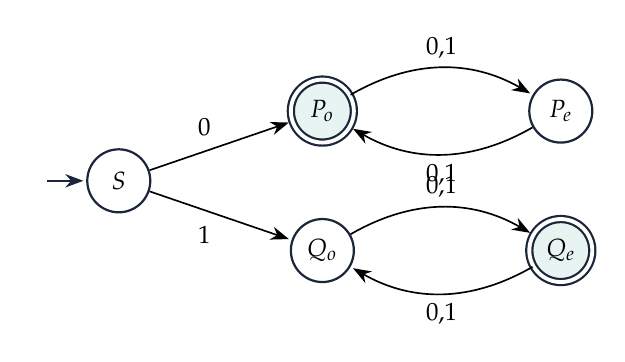
\begin{tikzpicture}[aut,node distance=22mm]
 \node[state,initial] (S) {$S$};
 \node[state,accepting] (O0) [above right=3mm and 20mm of S] {$P_o$}; \node[state] (E0) [right=of O0] {$P_e$};
 \node[state] (O1) [below right=3mm and 20mm of S] {$Q_o$}; \node[state,accepting] (E1) [right=of O1] {$Q_e$};
 \path (S) edge node {0} (O0) (S) edge node[swap] {1} (O1) (O0) edge[bend left] node {0,1} (E0) (E0) edge[bend left] node {0,1} (O0)
  (O1) edge[bend left] node {0,1} (E1) (E1) edge[bend left] node {0,1} (O1);
\end{tikzpicture}\end{minipage}
\begin{minipage}{.35\linewidth}\centering\small
\begin{tabular}{c|cc}\toprule&0&1\\\midrule $\to S$&$P_o$&$Q_o$\\ $*P_o$&$P_e$&$P_e$\\ $P_e$&$P_o$&$P_o$\\ $Q_o$&$Q_e$&$Q_e$\\ $*Q_e$&$Q_o$&$Q_o$\\\bottomrule\end{tabular}\end{minipage}\end{center}
$P$ = started with 0, $Q$ = started with 1; subscript = parity of the length so far.
\end{solution}

%-------------------------------------------------------------------
\begin{question}{2006--2007 \textbullet\ Q2(b)}{Source M01}{8}
Design a DFA for $L=\{w\mid w \text{ has an even number of 0's and an odd number of 1's}\}$. Verify it by finding $\hat\delta(q_0,11010)$, where $q_0$ is the start state.
\end{question}
\begin{solution}
Four states, one for each pair of parities: $q_0=(E,E)$, $q_1=(E,O)$, $q_2=(O,E)$, $q_3=(O,O)$ (parity of 0's, parity of 1's). 0 flips the first parity, 1 flips the second. Accept $q_1$.
\fig{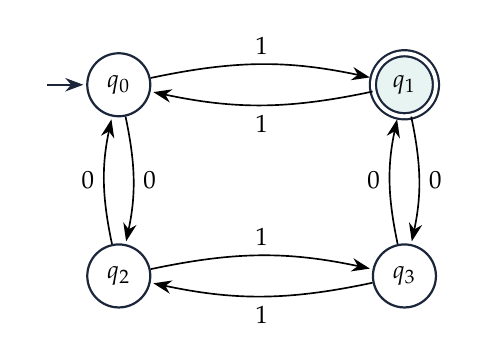
\begin{tikzpicture}[aut,node distance=28mm]
 \node[state,initial] (0) {$q_0$}; \node[state,accepting] (1) [right=of 0] {$q_1$};
 \node[state] (2) [below=16mm of 0] {$q_2$}; \node[state] (3) [right=of 2] {$q_3$};
 \path (0) edge[bend left=12] node {1} (1) (1) edge[bend left=12] node {1} (0) (2) edge[bend left=12] node {1} (3) (3) edge[bend left=12] node {1} (2)
  (0) edge[bend left=12] node {0} (2) (2) edge[bend left=12] node {0} (0) (1) edge[bend left=12] node {0} (3) (3) edge[bend left=12] node {0} (1);
\end{tikzpicture}}
\[
\hat\delta(q_0,\texttt{11010}):\ q_0\xrightarrow{1}q_1\xrightarrow{1}q_0\xrightarrow{0}q_2\xrightarrow{1}q_3\xrightarrow{0}q_1 .
\]
$\hat\delta(q_0,11010)=q_1\in F$, so it is accepted --- correct, since 11010 has two 0's (even) and three 1's (odd).
\end{solution}

\topic{03}{NFA design, \texorpdfstring{$\varepsilon$}{epsilon}-transitions and conversion}

%-------------------------------------------------------------------
\begin{question}{2023--2024 \textbullet\ Q3(a)}{Source N02}{15}
Find a three-state NFA for $L=\{a^n\mid n\ge1\}\cup\{b^ma^k\mid m,k\ge0\}$. Give only the diagram. Can an NFA with fewer than three states accept it? Elaborate.
\end{question}
\begin{solution}
\textbf{Three-state NFA} (one branch per part of the union, sharing the start):
\fig{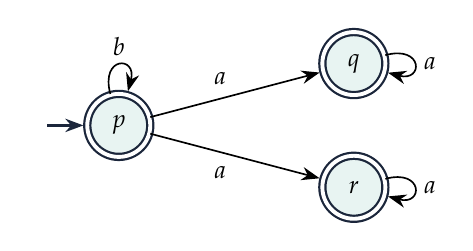
\begin{tikzpicture}[aut,node distance=22mm]
 \node[state,initial,accepting] (p) {$p$}; \node[state,accepting] (q) [above right=2mm and 24mm of p] {$q$}; \node[state,accepting] (r) [below right=2mm and 24mm of p] {$r$};
 \path (p) edge[loop above] node {$b$} () (p) edge node {$a$} (q) (q) edge[loop right] node {$a$} () (p) edge node[swap] {$a$} (r) (r) edge[loop right] node {$a$} ();
\end{tikzpicture}}
$p\xrightarrow{a}r\xrightarrow{a}\cdots$ gives $a^n$ ($n\ge1$); $p\xrightarrow{b^m}p\xrightarrow{a}q\xrightarrow{a^{k-1}}q$ gives $b^ma^k$.

\textbf{Fewer states?} Yes --- \emph{two} suffice. Observe $\{a^n\mid n\ge1\}\subseteq\{b^ma^k\}$ (take $m=0$), so $L=b^*a^*$, and state $r$ above is redundant:
\fig{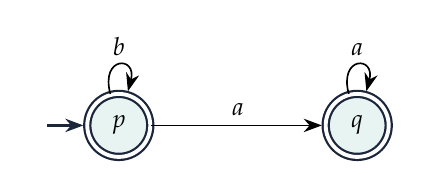
\begin{tikzpicture}[aut,node distance=22mm]
 \node[state,initial,accepting] (p) {$p$}; \node[state,accepting] (q) [right=of p] {$q$};
 \path (p) edge[loop above] node {$b$} () (p) edge node {$a$} (q) (q) edge[loop above] node {$a$} ();
\end{tikzpicture}}
\textbf{One state is impossible.} With one state $s$: since $\eps\in L$, $s$ must be accepting, so $L(N)=S^*$ where $S$ is the set of symbols on its self-loops. $S=\{a,b\}$ accepts $ab\notin L$; $S=\{a\}$ misses $b$; $S=\{b\}$ misses $a$; $S=\emptyset$ gives $\{\eps\}$. Hence the minimum is \textbf{2 states}.
\end{solution}

%-------------------------------------------------------------------
\begin{question}{2023--2024 \textbullet\ Q4(a)}{Source N02}{10}
Find an NFA accepting $\{a\}^*$ such that removing just one edge, with no other changes, makes it accept $\{a\}$. Give only the state diagram.
\end{question}
\begin{solution}
\fig{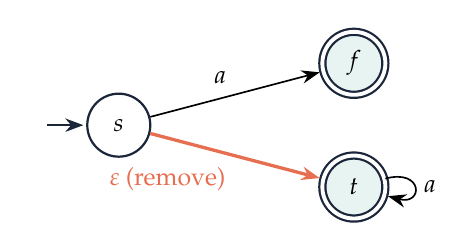
\begin{tikzpicture}[aut,node distance=24mm]
 \node[state,initial] (s) {$s$}; \node[state,accepting] (f) [above right=2mm and 24mm of s] {$f$}; \node[state,accepting] (t) [below right=2mm and 24mm of s] {$t$};
 \path (s) edge node {$a$} (f) (s) edge[draw=coral,very thick] node[swap,text=coral] {$\eps$\ (remove)} (t) (t) edge[loop right] node {$a$} ();
\end{tikzpicture}}
With the coral $\eps$-edge, $L=\{a\}\cup a^*=a^*$. Removing it leaves only $s\xrightarrow{a}f$, so $L=\{a\}$. (The removable edge must be an $\eps$-edge: $\eps\in a^*$ but $\eps\notin\{a\}$, and an accepting path for $\eps$ uses only $\eps$-edges.)
\end{solution}

%-------------------------------------------------------------------
\begin{question}{2022--2023 \textbullet\ Q4(b)}{Source M51}{15}
Draw an NFA for binary strings beginning and ending with different symbols and having odd length. A state diagram suffices.
\end{question}
\begin{solution}
Branch on the first symbol, track length parity, and guess that the next symbol is the last one --- allowed only when it differs from the first symbol and makes the length odd (i.e.\ it is read from an even-length state).
\fig{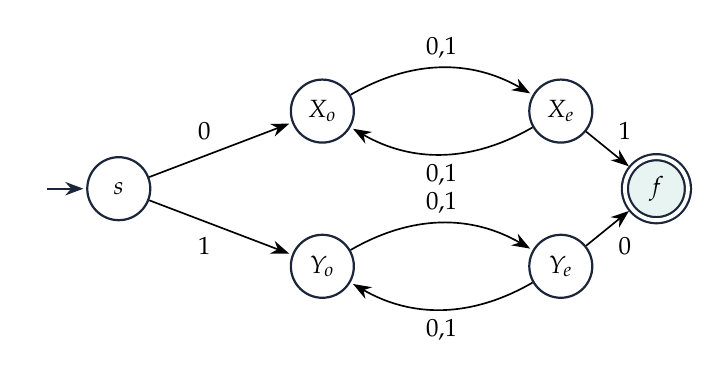
\begin{tikzpicture}[aut,node distance=22mm]
 \node[state,initial] (s) {$s$};
 \node[state] (Xo) [above right=4mm and 20mm of s] {$X_o$}; \node[state] (Xe) [right=of Xo] {$X_e$};
 \node[state] (Yo) [below right=4mm and 20mm of s] {$Y_o$}; \node[state] (Ye) [right=of Yo] {$Y_e$};
 \node[state,accepting] (f) [right=60mm of s] {$f$};
 \path (s) edge node {0} (Xo) (s) edge node[swap] {1} (Yo)
  (Xo) edge[bend left] node {0,1} (Xe) (Xe) edge[bend left] node {0,1} (Xo) (Xe) edge node {1} (f)
  (Yo) edge[bend left] node {0,1} (Ye) (Ye) edge[bend left] node {0,1} (Yo) (Ye) edge node[swap] {0} (f);
\end{tikzpicture}}
$X$: began with 0, $Y$: began with 1; subscript = parity of the length read so far. Example: $001$: $s\to X_o\to X_e\to f$ \ok; $01$ (even length) cannot reach $f$.
\end{solution}

%-------------------------------------------------------------------
\begin{question}{2021--2022 \textbullet\ Q2(b)}{Source M45}{10}
Using basic principles, convert $(((00)^*(11))\cup01)^*$ into an NFA.
\end{question}
\begin{solution}
Build bottom-up with the slide (Sipser) constructions: a symbol $x$ is the two-state NFA $q\xrightarrow{x}q'$ ($q'$ accepting), and every concatenation joins the pieces by an $\eps$-edge.
\begin{enumerate}
\item $00$: $a_1\xrightarrow0a_2\xrightarrow\eps b_1\xrightarrow0b_2$ (accepting $b_2$). \quad $(00)^*$: new accepting start $S_1$, $S_1\xrightarrow\eps a_1$, $b_2\xrightarrow\eps a_1$; accepting $S_1,b_2$.
\item $11$: $d_1\xrightarrow1d_2\xrightarrow\eps e_1\xrightarrow1e_2$. \quad $(00)^*11$: $\eps$-edges from the accepting states $S_1,b_2$ of $(00)^*$ to $d_1$; only $e_2$ accepts.
\item $01$: $g_1\xrightarrow0g_2\xrightarrow\eps h_1\xrightarrow1h_2$. \quad Union: new start $U$ with $U\xrightarrow\eps S_1$, $U\xrightarrow\eps g_1$; accepting $e_2,h_2$.
\item Star: new accepting start $S_0$, $S_0\xrightarrow\eps U$, and $e_2\xrightarrow\eps U$, $h_2\xrightarrow\eps U$. Accepting: $S_0,e_2,h_2$.
\end{enumerate}
\fig{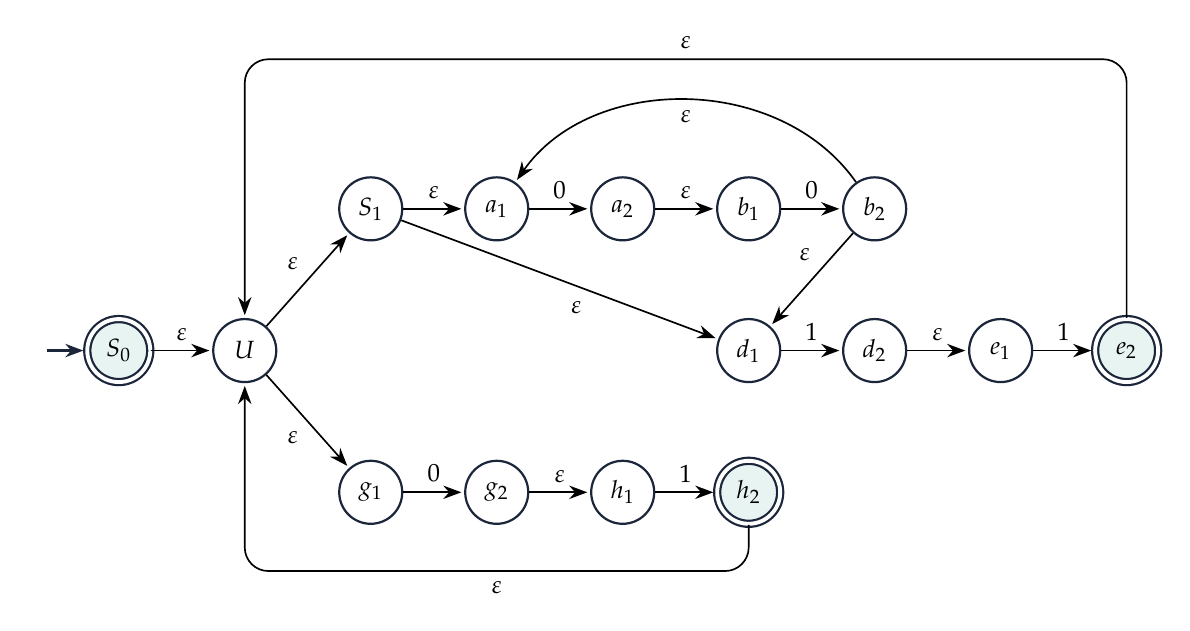
\begin{tikzpicture}[aut]
 \node[state,initial,accepting] (S0) at (0,0) {$S_0$}; \node[state] (U) at (1.6,0) {$U$};
 \node[state] (S1) at (3.2,1.8) {$S_1$}; \node[state] (a1) at (4.8,1.8) {$a_1$}; \node[state] (a2) at (6.4,1.8) {$a_2$}; \node[state] (b1) at (8,1.8) {$b_1$}; \node[state] (b2) at (9.6,1.8) {$b_2$};
 \node[state] (d1) at (8,0) {$d_1$}; \node[state] (d2) at (9.6,0) {$d_2$}; \node[state] (e1) at (11.2,0) {$e_1$}; \node[state,accepting] (e2) at (12.8,0) {$e_2$};
 \node[state] (g1) at (3.2,-1.8) {$g_1$}; \node[state] (g2) at (4.8,-1.8) {$g_2$}; \node[state] (h1) at (6.4,-1.8) {$h_1$}; \node[state,accepting] (h2) at (8,-1.8) {$h_2$};
 \path (S0) edge node {$\eps$} (U) (U) edge node {$\eps$} (S1) (U) edge node[swap] {$\eps$} (g1)
  (S1) edge node {$\eps$} (a1) (a1) edge node {0} (a2) (a2) edge node {$\eps$} (b1) (b1) edge node {0} (b2) (b2) edge[out=125,in=55] node {$\eps$} (a1)
  (S1) edge node[swap,pos=.6] {$\eps$} (d1) (b2) edge node[swap,pos=.4] {$\eps$} (d1)
  (d1) edge node {1} (d2) (d2) edge node {$\eps$} (e1) (e1) edge node {1} (e2)
  (g1) edge node {0} (g2) (g2) edge node {$\eps$} (h1) (h1) edge node {1} (h2);
 \draw[rounded corners=3mm] (e2.north) -- (12.8,3.7) -- node[above] {$\eps$} (1.6,3.7) -- (U.north);
 \draw[rounded corners=3mm] (h2.south) -- (8,-2.8) -- node[below] {$\eps$} (1.6,-2.8) -- (U.south);
\end{tikzpicture}}
\end{solution}

%-------------------------------------------------------------------
\begin{question}{2021--2022 \textbullet\ Q3(b)}{Source M45}{10}
Draw an NFA accepting binary strings containing at least two 0's or exactly two 1's. A state diagram suffices.
\end{question}
\begin{solution}
Union of two simple machines via a new start state with $\eps$-edges.
\fig{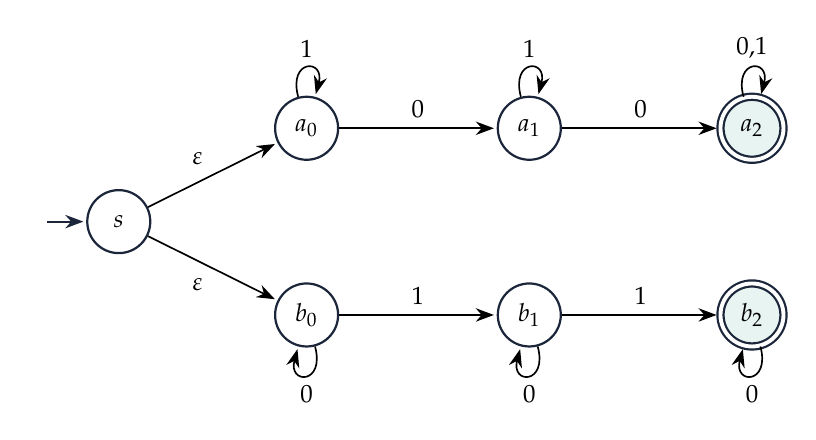
\begin{tikzpicture}[aut,node distance=20mm]
 \node[state,initial] (s) {$s$};
 \node[state] (a0) [above right=6mm and 18mm of s] {$a_0$}; \node[state] (a1) [right=of a0] {$a_1$}; \node[state,accepting] (a2) [right=of a1] {$a_2$};
 \node[state] (b0) [below right=6mm and 18mm of s] {$b_0$}; \node[state] (b1) [right=of b0] {$b_1$}; \node[state,accepting] (b2) [right=of b1] {$b_2$};
 \path (s) edge node {$\eps$} (a0) (s) edge node[swap] {$\eps$} (b0)
  (a0) edge[loop above] node {1} () (a0) edge node {0} (a1) (a1) edge[loop above] node {1} () (a1) edge node {0} (a2) (a2) edge[loop above] node {0,1} ()
  (b0) edge[loop below] node {0} () (b0) edge node {1} (b1) (b1) edge[loop below] node {0} () (b1) edge node {1} (b2) (b2) edge[loop below] node {0} ();
\end{tikzpicture}}
Upper branch counts 0's up to 2; lower branch counts 1's and has no move on a third 1 (that branch dies).
\end{solution}

%-------------------------------------------------------------------
\begin{question}{2021--2022 \textbullet\ Q3(c)}{Source M45--M46}{9}
Convert the given NFA into a DFA. Only the DFA state diagram is required.
\begin{center}\small\begin{tabular}{c|ccc}\toprule State&$a$&$b$&$\eps$\\\midrule $q_1$&$\{q_3\}$&$\emptyset$&$\{q_2\}$\\ $q_2$&$\{q_1\}$&$\emptyset$&$\emptyset$\\ $q_3$&$\{q_2\}$&$\{q_2,q_3\}$&$\emptyset$\\\bottomrule\end{tabular}\end{center}
\end{question}
\begin{solution}
\begin{note}The table marks neither start nor accepting states. This is the NFA of Sipser Exercise 1.16(b), whose start state is $q_1$ and accepting state is $q_2$; we use that.\end{note}
\sub{Step 1: remove the $\eps$-transitions}
$\delta'(q,x)=E\big(\bigcup_{r\in E(q)}\delta(r,x)\big)$ and $F'=\{q\mid E(q)\cap F\neq\emptyset\}$ with $F=\{q_2\}$:
\begin{center}\small\begin{tabular}{c|c|cc}\toprule $q$ & $E(q)$ & $\delta'(q,a)$ & $\delta'(q,b)$\\\midrule
$*q_1$ & $\{q_1,q_2\}$ & $E(\{q_3,q_1\})=\{q_1,q_2,q_3\}$ & $\emptyset$\\
$*q_2$ & $\{q_2\}$ & $E(\{q_1\})=\{q_1,q_2\}$ & $\emptyset$\\
$q_3$ & $\{q_3\}$ & $E(\{q_2\})=\{q_2\}$ & $E(\{q_2,q_3\})=\{q_2,q_3\}$\\\bottomrule\end{tabular}\end{center}
$F'=\{q_1,q_2\}$ ($q_1$ reaches $q_2$ by an $\eps$-move).
\sub{Step 2: subset construction from $\{q_1\}$}
$\delta_D(R,x)=\bigcup_{r\in R}\delta'(r,x)$; a subset is accepting iff it meets $F'$. Only reachable subsets are built:
\begin{center}\small\begin{tabular}{l|cc}\toprule DFA state & $a$ & $b$\\\midrule
$\to *\{q_1\}$ & $\{q_1,q_2,q_3\}$ & $\emptyset$\\
$*\{q_1,q_2,q_3\}$ & $\{q_1,q_2,q_3\}$ & $\emptyset\cup\emptyset\cup\{q_2,q_3\}=\{q_2,q_3\}$\\
$*\{q_2,q_3\}$ & $\{q_1,q_2\}\cup\{q_2\}=\{q_1,q_2\}$ & $\{q_2,q_3\}$\\
$*\{q_1,q_2\}$ & $\{q_1,q_2,q_3\}$ & $\emptyset$\\
$\emptyset$ & $\emptyset$ & $\emptyset$\\\bottomrule\end{tabular}\end{center}
\fig{\begin{tikzpicture}[aut]
 \node[state,initial,accepting] (A) at (0,0) {$\{1\}$}; \node[state,accepting] (B) at (3,0) {$\{1,2,3\}$}; \node[state,accepting] (C) at (6,0) {$\{2,3\}$};
 \node[state,accepting] (D) at (4.5,-2.3) {$\{1,2\}$}; \node[state,dead] (E) at (0,-2.3) {$\emptyset$};
 \path (A) edge node {$a$} (B) (B) edge[loop above] node {$a$} () (B) edge node {$b$} (C) (C) edge[loop above] node {$b$} ()
  (C) edge node {$a$} (D) (D) edge node {$a$} (B) (D) edge node {$b$} (E)
  (A) edge node[swap] {$b$} (E) (E) edge[loop left] node {$a,b$} ();
\end{tikzpicture}}
Five reachable states (numbers abbreviate $q_i$); all except $\emptyset$ are accepting.
\end{solution}

%-------------------------------------------------------------------
\begin{question}{2019--2020 \textbullet\ Q3(a)}{Source M40}{5}
Construct an NFA for $((a^*)a)^*$ using basic principles.
\end{question}
\begin{solution}
$a$: $x\xrightarrow a y$. $\ a^*$: new accepting start $S_1$, $S_1\xrightarrow\eps x$, $y\xrightarrow\eps x$. $\ (a^*)a$: $\eps$ from $S_1,y$ to $z\xrightarrow a t$. $\ ((a^*)a)^*$: new accepting start $S_0\xrightarrow\eps S_1$, $t\xrightarrow\eps S_1$.
\fig{\begin{tikzpicture}[aut,node distance=17mm]
 \node[state,initial,accepting] (S0) {$S_0$}; \node[state] (S1) [right=of S0] {$S_1$}; \node[state] (x) [right=of S1] {$x$}; \node[state] (y) [right=of x] {$y$};
 \node[state] (z) [right=of y] {$z$}; \node[state,accepting] (t) [right=of z] {$t$};
 \path (S0) edge node {$\eps$} (S1) (S1) edge node {$\eps$} (x) (x) edge node {$a$} (y) (y) edge[bend right=40] node[swap] {$\eps$} (x)
  (y) edge node {$\eps$} (z) (S1) edge[bend right=30] node[swap] {$\eps$} (z) (z) edge node {$a$} (t) (t) edge[bend right=40] node[swap] {$\eps$} (S1);
\end{tikzpicture}}
(The language is simply $a^*$, but the question asks for the systematic construction.)
\end{solution}

%-------------------------------------------------------------------
\begin{question}{2019--2020 \textbullet\ Q3(b)}{Source M40}{15}
Design an NFA for $L=\{a^nb^n\mid n\le3\}$ over $\{a,b\}$. Give only a state diagram. Using more than the required minimum states may be penalized.
\end{question}
\begin{solution}
$L=\{\eps,ab,aabb,aaabbb\}$. After $k$ $a$'s jump to the point of the $b$-chain that still needs $k$ $b$'s:
\fig{\begin{tikzpicture}[aut,node distance=18mm]
 \node[state,initial,accepting] (0) {$A_0$}; \node[state] (1) [right=of 0] {$A_1$}; \node[state] (2) [right=of 1] {$A_2$}; \node[state] (3) [right=of 2] {$A_3$};
 \node[state] (B2) [below=14mm of 3] {$B_2$}; \node[state] (B1) [left=of B2] {$B_1$}; \node[state,accepting] (F) [left=of B1] {$F$};
 \path (0) edge node {$a$} (1) (1) edge node {$a$} (2) (2) edge node {$a$} (3) (3) edge node {$b$} (B2) (B2) edge node {$b$} (B1) (B1) edge node {$b$} (F)
  (2) edge node[swap] {$b$} (B1) (1) edge node[swap] {$b$} (F);
\end{tikzpicture}}
\textbf{Fewer than 7 states is impossible.} Let $N$ be any NFA with $L(N)=L$. Since $a^3b^3=s_1s_2\cdots s_6\in L$, $N$ has an accepting computation on it; let $r_i$ be the state it is in after reading the first $i$ symbols ($i=0,1,\dots,6$). Suppose $r_i=r_j$ for some $i<j$. Then the part of the computation between these two moments reads the $j-i\ge1$ symbols $s_{i+1}\cdots s_j$ and returns to the same state, so it can be traversed twice: $N$ also accepts $s_1\cdots s_i\,(s_{i+1}\cdots s_j)^2\,s_{j+1}\cdots s_6$, a string of length $6+(j-i)>6$. But every string of $L$ has length at most 6 --- contradiction. Hence $r_0,\dots,r_6$ are 7 different states, and every NFA for $L$ has at least 7 states; the NFA above is optimal.
\end{solution}

%-------------------------------------------------------------------
\begin{question}{2019--2020 \textbullet\ Q4(a)}{Source M41}{5}
When a five-state NFA is converted to a DFA, what are the minimum and maximum possible numbers of DFA states? Justify.
\end{question}
\begin{solution}
Each DFA state of the subset construction is a subset of the 5 NFA states, so there are at most $2^5=\mathbf{32}$ states (counting $\emptyset$). The bound is attainable. Example: states $0,\dots,4$, start $0$, alphabet $\{a,b,c\}$ with $a$: $i\mapsto\{i+1 \bmod 5\}$; $b$: $0\mapsto\{0,1\}$, $i\mapsto\{i\}$ for $i\neq0$; $c$: $0\mapsto\emptyset$, $i\mapsto\{i\}$ for $i\neq0$. In the subset construction $a$ rotates a subset, $b$ adds $1$ to a subset containing $0$, and $c$ deletes $0$. From $\{0\}$ the word $(ba^4)^3b$ reaches $\{0,1,2,3,4\}$, and any element $j$ can then be deleted by $a^{5-j}ca^{j}$ (rotate $j$ to $0$, delete, rotate back). So all $32$ subsets are reachable DFA states.
At least \textbf{1} state is always needed, and 1 can happen: e.g.\ an NFA whose start state is accepting with self-loops on every symbol (accepts $\Sigma^*$) yields the single DFA state $E(\{q_0\})$, which maps to itself.
\ans{Minimum 1, maximum $2^5=32$.}
\end{solution}

%-------------------------------------------------------------------
\repeated{3}
\begin{question}{January 2020 Term \textbullet\ Q1(c)}{Source M36}{12}
For the given NFA, give general forms of all accepted strings of length at most 3, with explanations.
\begin{center}\small\begin{tabular}{c|cccc}\toprule State&$a$&$b$&$c$&$\eps$\\\midrule $\to p$&$\{p\}$&$\{q\}$&$\{r\}$&$\emptyset$\\ $q$&$\{q\}$&$\{r\}$&$\emptyset$&$\{p\}$\\ $*r$&$\{r\}$&$\emptyset$&$\{p\}$&$\{q\}$\\\bottomrule\end{tabular}\end{center}
\end{question}
\begin{question}{2017--2018 \textbullet\ Q4(a)}{Source M33}{15}
For the given NFA (same table as above): (i) give, with explanations, general forms of every accepted string of length at most 3; (ii) convert it to a DFA (detailed computations optional).
\end{question}
\begin{question}{2008--2009 \textbullet\ Q6(c)}{Source M07}{5$\tfrac13$}
For the $\eps$-NFA in the table: (i) compute the $\eps$-closure of each state; (ii) convert it to a DFA.
\begin{center}\small\begin{tabular}{c|cccc}\toprule State&$\eps$&$a$&$b$&$c$\\\midrule $\to p$&$\emptyset$&$\{p\}$&$\{q\}$&$\{r\}$\\ $q$&$\{p\}$&$\{q\}$&$\{r\}$&$\emptyset$\\ $*r$&$\{q\}$&$\{r\}$&$\emptyset$&$\{p\}$\\\bottomrule\end{tabular}\end{center}
\end{question}
\begin{solution}
\scope{January 2020 Term Q1(c) asks only for the accepted strings of length $\le3$ (last part); 2008--2009 Q6(c) asks only for the $\eps$-closures and the DFA (Steps 1--2); 2017--2018 Q4(a) asks for the strings of length $\le3$ and the DFA.}
All three tables describe the \emph{same} $\eps$-NFA (only the column order differs).
\fig{\begin{tikzpicture}[aut,node distance=28mm]
 \node[state,initial] (p) {$p$}; \node[state] (q) [right=of p] {$q$}; \node[state,accepting] (r) [right=of q] {$r$};
 \path (p) edge[loop above] node {$a$} () (q) edge[loop above] node {$a$} () (r) edge[loop above] node {$a$} ()
  (p) edge[bend left=15] node {$b$} (q) (q) edge[bend left=15] node {$\eps$} (p) (q) edge[bend left=15] node {$b$} (r) (r) edge[bend left=15] node {$\eps$} (q)
  (p) edge[bend right=40] node[swap] {$c$} (r) (r) edge[bend right=-60,looseness=1.1] node {$c$} (p);
 \end{tikzpicture}}
\sub{Step 1: $\eps$-closures and removal of the $\eps$-transitions}
$E(p)=\{p\}$,\quad $E(q)=\{q,p\}$,\quad $E(r)=\{r,q,p\}$. With $\delta'(s,x)=E\big(\bigcup_{t\in E(s)}\delta(t,x)\big)$ and $F'=\{s\mid E(s)\cap F\neq\emptyset\}$:
\begin{center}\small\begin{tabular}{c|ccc}\toprule & $a$ & $b$ & $c$\\\midrule
$\to p$ & $E(\{p\})=\{p\}$ & $E(\{q\})=\{p,q\}$ & $E(\{r\})=\{p,q,r\}$\\
$q$ & $E(\{p,q\})=\{p,q\}$ & $E(\{q,r\})=\{p,q,r\}$ & $E(\{r\})=\{p,q,r\}$\\
$*r$ & $E(\{p,q,r\})=\{p,q,r\}$ & $E(\{q,r\})=\{p,q,r\}$ & $E(\{r,p\})=\{p,q,r\}$\\\bottomrule\end{tabular}\end{center}
$F'=\{r\}$ (neither $E(p)$ nor $E(q)$ contains $r$).
\sub{Step 2: subset construction from $\{p\}$}
$\delta_D(R,x)=\bigcup_{s\in R}\delta'(s,x)$, reachable subsets only:
\begin{center}\small\begin{tabular}{l|ccc}\toprule & $a$ & $b$ & $c$\\\midrule
$\to A=\{p\}$ & $\{p\}=A$ & $\{p,q\}=B$ & $\{p,q,r\}=C$\\
$B=\{p,q\}$ & $\{p,q\}=B$ & $\{p,q\}\cup\{p,q,r\}=C$ & $C$\\
$*C=\{p,q,r\}$ & $C$ & $C$ & $C$\\\bottomrule\end{tabular}\end{center}
\fig{\begin{tikzpicture}[aut,node distance=28mm]
 \node[state,initial] (A) {$\{p\}$}; \node[state] (B) [right=of A] {$\{p,q\}$}; \node[state,accepting] (C) [right=of B] {$\{p,q,r\}$};
 \path (A) edge[loop above] node {$a$} () (A) edge node {$b$} (B) (B) edge[loop above] node {$a$} () (B) edge node {$b,c$} (C)
  (A) edge[bend right=30] node[swap] {$c$} (C) (C) edge[loop above] node {$a,b,c$} ();
\end{tikzpicture}}
So $L=\{w\in\{a,b,c\}^*\mid w \text{ contains a } c \text{ or at least two } b\text{'s}\}$.
\sub{Accepted strings of length $\le3$ (general forms)}
Reading $a$ never changes the DFA state; one $b$ moves $\{p\}\to\{p,q\}$; a second $b$ or any $c$ reaches the accepting sink.
\begin{itemize}
\item Length 0, 1: $\eps$ is rejected; of length 1 only $c$.
\item Length 2: $xc$ and $cx$ for any $x\in\{a,b,c\}$, and $bb$ --- i.e.\ $\{ac,bc,cc,ca,cb,bb\}$.
\item Length 3: \emph{every} string containing at least one $c$ (19 strings: $\Sigma^3$ minus the 8 strings over $\{a,b\}$), plus $abb$, $bab$, $bba$, $bbb$ (the strings over $\{a,b\}$ with $\ge2$ $b$'s) --- 23 strings in total.
\end{itemize}
\end{solution}

%-------------------------------------------------------------------
\begin{question}{January 2020 Term \textbullet\ Q2(b)}{Source M36}{13}
Draw an equivalent NFA for the DFA in 2(a) (the five-state DFA accepting strings that end in $00$ or $11$; see Topic 01).
\end{question}
\begin{solution}
The DFA accepts $(0\cup1)^*(00\cup11)$. An NFA simply guesses where the final pair starts:
\fig{\begin{tikzpicture}[aut,node distance=22mm]
 \node[state,initial] (s) {$s$}; \node[state] (z) [above right=2mm and 22mm of s] {$z$}; \node[state] (o) [below right=2mm and 22mm of s] {$o$};
 \node[state,accepting] (f) [right=46mm of s] {$f$};
 \path (s) edge[loop above] node {0,1} () (s) edge node {0} (z) (z) edge node {0} (f) (s) edge node[swap] {1} (o) (o) edge node[swap] {1} (f);
\end{tikzpicture}}
4 states instead of 5, with one nondeterministic choice at $s$ for each symbol.
\end{solution}

%-------------------------------------------------------------------
\begin{question}{January 2020 Term \textbullet\ Q4(b)}{Source M37}{20}
Convert the shown NFA to an equivalent DFA, showing computations.
\fig{\begin{tikzpicture}[aut,node distance=13mm]
 \node[state,initial] (0) {$q_0$}; \node[state] (1) [right=of 0] {$q_1$};
 \node[state] (2) [above right=6mm and 9mm of 1] {$q_2$}; \node[state] (3) [right=of 2] {$q_3$};
 \node[state] (4) [below right=6mm and 9mm of 1] {$q_4$}; \node[state] (5) [right=of 4] {$q_5$};
 \node[state] (6) [below right=6mm and 9mm of 3] {$q_6$}; \node[state] (7) [right=of 6] {$q_7$};
 \node[state] (8) [right=of 7] {$q_8$}; \node[state] (9) [right=of 8] {$q_9$}; \node[state,accepting] (10) [right=of 9] {$q_{10}$};
 \path (0) edge node {$\eps$} (1) (1) edge node {$\eps$} (2) (1) edge node[swap] {$\eps$} (4) (2) edge node {0} (3) (4) edge node {1} (5)
  (3) edge node {$\eps$} (6) (5) edge node[swap] {$\eps$} (6) (6) edge[bend right=75,looseness=1.4] node[swap] {$\eps$} (1) (6) edge node {$\eps$} (7)
  (7) edge node {0} (8) (8) edge node {1} (9) (9) edge node {1} (10) (0) edge[bend right=40] node[swap] {$\eps$} (7);
\end{tikzpicture}}
\end{question}
\begin{solution}
(This NFA recognizes $(0\cup1)^*011$. Numbers abbreviate $q_i$.)
\sub{Step 1: remove the $\eps$-transitions}
$\delta'(q,x)=E\big(\bigcup_{r\in E(q)}\delta(r,x)\big)$, $F'=\{q\mid E(q)\ni q_{10}\}=\{q_{10}\}$ (no other state reaches $q_{10}$ by $\eps$-moves alone):
\begin{center}\small\begin{tabular}{c|l|l|l}\toprule $q$ & $E(q)$ & $\delta'(q,0)$ & $\delta'(q,1)$\\\midrule
$\to0$ & $\{0,1,2,4,7\}$ & $E(\{3,8\})=\{1,2,3,4,6,7,8\}$ & $E(\{5\})=\{1,2,4,5,6,7\}$\\
$1$ & $\{1,2,4\}$ & $E(\{3\})=\{1,2,3,4,6,7\}$ & $\{1,2,4,5,6,7\}$\\
$2$ & $\{2\}$ & $\{1,2,3,4,6,7\}$ & $\emptyset$\\
$3$ & $\{1,2,3,4,6,7\}$ & $\{1,2,3,4,6,7,8\}$ & $\{1,2,4,5,6,7\}$\\
$4$ & $\{4\}$ & $\emptyset$ & $\{1,2,4,5,6,7\}$\\
$5$ & $\{1,2,4,5,6,7\}$ & $\{1,2,3,4,6,7,8\}$ & $\{1,2,4,5,6,7\}$\\
$6$ & $\{1,2,4,6,7\}$ & $\{1,2,3,4,6,7,8\}$ & $\{1,2,4,5,6,7\}$\\
$7$ & $\{7\}$ & $\{8\}$ & $\emptyset$\\
$8$ & $\{8\}$ & $\emptyset$ & $\{9\}$\\
$9$ & $\{9\}$ & $\emptyset$ & $\{10\}$\\
$*10$ & $\{10\}$ & $\emptyset$ & $\emptyset$\\\bottomrule\end{tabular}\end{center}
\sub{Step 2: subset construction from $\{q_0\}$}
$\delta_D(R,x)=\bigcup_{r\in R}\delta'(r,x)$, reachable subsets only:
\begin{center}\small\begin{tabular}{l|l|l}\toprule DFA state & on 0 & on 1\\\midrule
$\to A=\{0\}$ & $\{1,2,3,4,6,7,8\}=B$ & $\{1,2,4,5,6,7\}=C$\\
$B=\{1,2,3,4,6,7,8\}$ & $B$ & $\{1,2,4,5,6,7\}\cup\{9\}=\{1,2,4,5,6,7,9\}=D$\\
$C=\{1,2,4,5,6,7\}$ & $B$ & $C$\\
$D=\{1,2,4,5,6,7,9\}$ & $B$ & $\{1,2,4,5,6,7\}\cup\{10\}=\{1,2,4,5,6,7,10\}=F$\\
$*F=\{1,2,4,5,6,7,10\}$ & $B$ & $C$\\\bottomrule\end{tabular}\end{center}
Only $F$ contains $q_{10}\in F'$, so $F$ is the sole accepting state.
\fig{\begin{tikzpicture}[aut,node distance=22mm]
 \node[state,initial] (A) {$A$}; \node[state] (B) [right=of A] {$B$}; \node[state] (D) [right=of B] {$D$}; \node[state,accepting] (F) [right=of D] {$F$};
 \node[state] (C) [below=16mm of B] {$C$};
 \path (A) edge node {0} (B) (A) edge node[swap] {1} (C) (B) edge[loop above] node {0} () (B) edge node {1} (D) (D) edge node {1} (F)
  (D) edge[bend right=40] node[swap] {0} (B) (F) edge[bend right=50] node[swap] {0} (B) (F) edge[bend left=20] node {1} (C)
  (C) edge[loop below] node {1} () (C) edge[bend left=15] node {0} (B);
\end{tikzpicture}}
\end{solution}

%-------------------------------------------------------------------
\begin{question}{2017--2018 \textbullet\ Q2(c)}{Source M32}{8}
Using regular-language closure constructions, draw an NFA for $(a\cup b)^*aba$.
\end{question}
\begin{solution}
$a\cup b$: start $u$ with $u\xrightarrow\eps p_1\xrightarrow a p_2$ and $u\xrightarrow\eps r_1\xrightarrow b r_2$. Star: new accepting start $S$, $S\xrightarrow\eps u$, $p_2,r_2\xrightarrow\eps u$. Concatenate with $a$, $b$, $a$ (each a two-state NFA) using $\eps$-edges from the previous accepting states.
\fig{\begin{tikzpicture}[aut,node distance=13mm]
 \node[state,initial] (S) {$S$}; \node[state] (u) [right=of S] {$u$};
 \node[state] (p1) [above right=5mm and 9mm of u] {$p_1$}; \node[state] (p2) [right=of p1] {$p_2$};
 \node[state] (r1) [below right=5mm and 9mm of u] {$r_1$}; \node[state] (r2) [right=of r1] {$r_2$};
 \node[state] (x1) [right=38mm of u] {$x_1$}; \node[state] (x2) [right=of x1] {$x_2$}; \node[state] (x3) [right=of x2] {$x_3$}; \node[state] (x4) [right=of x3] {$x_4$}; \node[state] (x5) [right=of x4] {$x_5$}; \node[state,accepting] (x6) [right=of x5] {$x_6$};
 \path (S) edge node {$\eps$} (u) (u) edge node {$\eps$} (p1) (u) edge node[swap] {$\eps$} (r1) (p1) edge node {$a$} (p2) (r1) edge node {$b$} (r2)
  (p2) edge[bend right=60] node[swap,pos=.6] {$\eps$} (u) (r2) edge[bend left=60] node[pos=.6] {$\eps$} (u)
  (p2) edge node {$\eps$} (x1) (r2) edge node[swap] {$\eps$} (x1) (S) edge[bend right=55,looseness=.9] node[swap] {$\eps$} (x1)
  (x1) edge node {$a$} (x2) (x2) edge node {$\eps$} (x3) (x3) edge node {$b$} (x4) (x4) edge node {$\eps$} (x5) (x5) edge node {$a$} (x6);
\end{tikzpicture}}
(After removing $\eps$-moves this collapses to the familiar 4-state NFA $s\xrightarrow{a,b}s$, $s\xrightarrow a 1\xrightarrow b 2\xrightarrow a 3$.)
\end{solution}

%-------------------------------------------------------------------
\begin{question}{2017--2018 \textbullet\ Q3(a)}{Source M32}{18}
Design an NFA for binary strings containing two 0's with a nonzero multiple of 4 characters between them; other 0's may occur. Give a state diagram and transition table. Source accepted examples: 00000, 101111010, 01000010111011. Source rejected examples: 00, 10101010.
\end{question}
\begin{solution}
\begin{note}With the stated condition, $00000$ should be \emph{rejected}: any two of its 0's have $0,1,2$ or $3$ characters between them, never a nonzero multiple of 4. The NFA below follows the stated condition; the other four examples are handled correctly.\end{note}
Guess the first of the two 0's, then count the characters after it modulo 4 (at least 4 of them), and guess that a 0 read when the count is $\equiv0$ (and $\ge4$) is the second one.
\fig{\begin{tikzpicture}[aut,node distance=16mm]
 \node[state,initial] (s) {$s$}; \node[state] (c0) [right=of s] {$c_0$}; \node[state] (c1) [right=of c0] {$c_1$}; \node[state] (c2) [right=of c1] {$c_2$}; \node[state] (c3) [right=of c2] {$c_3$}; \node[state] (c4) [right=of c3] {$c_4$};
 \node[state,accepting] (F) [right=of c4] {$F$};
 \path (s) edge[loop above] node {0,1} () (s) edge node {0} (c0) (c0) edge node {0,1} (c1) (c1) edge node {0,1} (c2) (c2) edge node {0,1} (c3) (c3) edge node {0,1} (c4)
  (c4) edge node {0} (F) (c4) edge[bend left=35] node[swap] {0,1} (c1) (F) edge[loop above] node {0,1} ();
\end{tikzpicture}}
\begin{center}\small\begin{tabular}{c|cc}\toprule State&0&1\\\midrule $\to s$&$\{s,c_0\}$&$\{s\}$\\ $c_0$&$\{c_1\}$&$\{c_1\}$\\ $c_1$&$\{c_2\}$&$\{c_2\}$\\ $c_2$&$\{c_3\}$&$\{c_3\}$\\ $c_3$&$\{c_4\}$&$\{c_4\}$\\ $c_4$&$\{F,c_1\}$&$\{c_1\}$\\ $*F$&$\{F\}$&$\{F\}$\\\bottomrule\end{tabular}\end{center}
$c_k$: $k$ characters read since the guessed first 0 ($c_4$ stands for any count $\equiv0\pmod4$, $\ge4$). Example $101111010$: 0 at position 2 $\to c_0$; $1111\to c_4$; next 0 $\to F$ \ok. $10101010$: gaps are 1, 3, 5 characters, never $\equiv0$, so $F$ is unreachable.
\end{solution}

%-------------------------------------------------------------------
\begin{question}{2016--2017 \textbullet\ Q2(b)}{Source M29}{8}
Convert the given NFA to an equivalent DFA. Detailed computations are optional.
\fig{\begin{tikzpicture}[aut,node distance=34mm]
 \node[state,initial] (p) {$p$}; \node[state,accepting] (q) [right=of p] {$q$}; \node[state] (s) [below=20mm of p] {$s$}; \node[state] (r) [below=20mm of q] {$r$};
 \path (p) edge node {0} (q) (q) edge[loop above] node {0} () (p) edge node[pos=.3] {$\eps$} (r) (q) edge[bend left=20] node {$\eps$} (r) (r) edge[bend left=20] node {1} (q)
  (s) edge node {0} (p) (s) edge[bend left=12] node {0} (r) (r) edge[bend left=12] node {$\eps$} (s);
\end{tikzpicture}}
\end{question}
\begin{solution}
\sub{Step 1: remove the $\eps$-transitions}
$\delta'(x,c)=E\big(\bigcup_{y\in E(x)}\delta(y,c)\big)$, $F'=\{x\mid E(x)\ni q\}=\{q\}$:
\begin{center}\small\begin{tabular}{c|c|ll}\toprule & $E(\cdot)$ & $\delta'(\cdot,0)$ & $\delta'(\cdot,1)$\\\midrule
$\to p$ & $\{p,r,s\}$ & $E(\{q,p,r\})=\{p,q,r,s\}$ & $E(\{q\})=\{q,r,s\}$\\
$*q$ & $\{q,r,s\}$ & $E(\{q,p,r\})=\{p,q,r,s\}$ & $E(\{q\})=\{q,r,s\}$\\
$r$ & $\{r,s\}$ & $E(\{p,r\})=\{p,r,s\}$ & $E(\{q\})=\{q,r,s\}$\\
$s$ & $\{s\}$ & $E(\{p,r\})=\{p,r,s\}$ & $\emptyset$\\\bottomrule\end{tabular}\end{center}
\sub{Step 2: subset construction from $\{p\}$}
$\delta_D(R,x)=\bigcup_{y\in R}\delta'(y,x)$, reachable subsets only:
\begin{center}\small\begin{tabular}{l|l|l}\toprule & 0 & 1\\\midrule
$\to A=\{p\}$ & $\{p,q,r,s\}=B$ & $\{q,r,s\}=C$\\
$*B=\{p,q,r,s\}$ & $\{p,q,r,s\}\cup\{p,r,s\}=B$ & $\{q,r,s\}\cup\emptyset=C$\\
$*C=\{q,r,s\}$ & $\{p,q,r,s\}\cup\{p,r,s\}=B$ & $\{q,r,s\}=C$\\\bottomrule\end{tabular}\end{center}
\fig{\begin{tikzpicture}[aut,node distance=28mm]
 \node[state,initial] (A) {$A$}; \node[state,accepting] (B) [above right=2mm and 26mm of A] {$B$}; \node[state,accepting] (C) [below right=2mm and 26mm of A] {$C$};
 \path (A) edge node {0} (B) (A) edge node[swap] {1} (C) (B) edge[loop right] node {0} () (C) edge[loop right] node {1} () (B) edge[bend left=15] node {1} (C) (C) edge[bend left=15] node {0} (B);
\end{tikzpicture}}
$A$ is non-accepting, so $\eps$ is rejected; every non-empty string leads to $B$ or $C$, both accepting (no edge returns to $A$), so the language is $(0\cup1)^+$: every non-empty string.
\end{solution}

%-------------------------------------------------------------------
\begin{question}{2016--2017 \textbullet\ Q3(a)}{Source M29}{5 + 8 + 7 = 20}
Draw NFAs for:
(i) strings over $\{0,1,\dots,9\}$ whose final digit appeared earlier;
(ii) strings over $\{0,1,\dots,9\}$ whose final digit did not appear earlier;
(iii) binary strings with at least two 0's separated by a number of positions divisible by 4. Other 0's may occur; zero is allowed as a multiple of 4. Accepted examples: 00, 10111010, 01010111011.
\end{question}
\begin{solution}
Let $\Sigma=\{0,\dots,9\}$; $\Sigma-d$ means every digit except $d$. Only the branches for digits $0$ and $9$ are drawn; the other eight are identical.
\sub{(i) Final digit appeared earlier}
\fig{\begin{tikzpicture}[aut,node distance=24mm]
 \node[state,initial] (s) {$s$}; \node[state] (p0) [above right=6mm and 24mm of s] {$p_0$}; \node[state] (p9) [below right=6mm and 24mm of s] {$p_9$};
 \node (dots) at ($(p0)!.5!(p9)$) {$\vdots$}; \node[state,accepting] (f) [right=58mm of s] {$f$};
 \path (s) edge[loop above] node {$\Sigma$} () (s) edge node {0} (p0) (s) edge node[swap] {9} (p9) (p0) edge[loop above] node {$\Sigma$} () (p9) edge[loop below] node {$\Sigma$} ()
  (p0) edge node {0} (f) (p9) edge node[swap] {9} (f);
\end{tikzpicture}}
Guess an earlier occurrence of digit $d$ (go to $p_d$), skip anything, then read $d$ as the final symbol ($f$ has no outgoing edges). 12 states.
\sub{(ii) Final digit did not appear earlier}
\fig{\begin{tikzpicture}[aut,node distance=24mm]
 \node[state,initial] (s) {$s$}; \node[state] (t0) [above right=6mm and 24mm of s] {$t_0$}; \node[state] (t9) [below right=6mm and 24mm of s] {$t_9$};
 \node (dots) at ($(t0)!.5!(t9)$) {$\vdots$}; \node[state,accepting] (f) [right=58mm of s] {$f$};
 \path (s) edge node {$\eps$} (t0) (s) edge node[swap] {$\eps$} (t9) (t0) edge[loop above] node {$\Sigma-0$} () (t9) edge[loop below] node {$\Sigma-9$} ()
  (t0) edge node {0} (f) (t9) edge node[swap] {9} (f);
\end{tikzpicture}}
Guess at the very beginning which digit $d$ will be last; read only digits $\ne d$, then $d$ once. Note the different design: in (ii) the guess is made \emph{first}, because ``did not appear'' must be checked on the whole prefix.
\sub{(iii) Two 0's separated by $\equiv0\pmod4$ symbols}
\begin{note}The text says the number of symbols \emph{between} the 0's is a multiple of 4 (so $00$, with 0 symbols between, is accepted). The other two examples instead have 0's whose \emph{positions} differ by a multiple of 4 (3, 7, \dots\ symbols between). We follow the stated condition and show the one-edge change for the other reading.\end{note}
\fig{\begin{tikzpicture}[aut,node distance=17mm]
 \node[state,initial] (s) {$s$}; \node[state] (c0) [right=of s] {$c_0$}; \node[state] (c1) [right=of c0] {$c_1$}; \node[state] (c2) [right=of c1] {$c_2$}; \node[state] (c3) [right=of c2] {$c_3$};
 \node[state,accepting] (F) [below=14mm of c0] {$F$};
 \path (s) edge[loop above] node {0,1} () (s) edge node {0} (c0) (c0) edge node {0,1} (c1) (c1) edge node {0,1} (c2) (c2) edge node {0,1} (c3) (c3) edge[bend right=35] node[swap] {0,1} (c0)
  (c0) edge node {0} (F) (F) edge[loop right] node {0,1} ();
\end{tikzpicture}}
$c_k$: number of symbols read since the first guessed 0 is $\equiv k\pmod 4$. A 0 read in $c_0$ has $0,4,8,\dots$ symbols before it since the first 0 $\Rightarrow F$. (For the ``position difference'' reading, replace the edge $c_0\xrightarrow0F$ by $c_3\xrightarrow0F$.)
\end{solution}

%-------------------------------------------------------------------
\begin{question}{2014--2015 \textbullet\ Q3(a)}{Source M22}{13$\tfrac13$}
Design an NFA over $\{a,b\}$ accepting nonempty strings with a nonzero even number of $a$'s at the end. Accept $aa$, $aaaa$, $abbaa$, $abaababaaaa$; reject $aaa$, $ab$, $b$, $abbaaa$, $abaabbbb$.
\end{question}
\begin{solution}
The trailing block of $a$'s must have even length $\ge2$. Track the parity of the current trailing block; a $b$ resets it. (A DFA is a special NFA.)
\fig{\begin{tikzpicture}[aut,node distance=24mm]
 \node[state,initial] (B) {$B$}; \node[state] (O) [right=of B] {$O$}; \node[state,accepting] (E) [right=of O] {$E$};
 \path (B) edge[loop above] node {$b$} () (B) edge node {$a$} (O) (O) edge[bend left] node {$a$} (E) (E) edge[bend left] node {$a$} (O)
  (O) edge[bend left=40] node {$b$} (B) (E) edge[bend left=55] node {$b$} (B);
\end{tikzpicture}}
$B$: no trailing $a$; $O$: odd trailing block; $E$: even ($\ge2$). Checks: $abbaaa$ ends in $O$ (3 $a$'s) reject; $abaababaaaa$ ends in $E$ (4 $a$'s) accept.
A genuinely nondeterministic alternative: $s\xrightarrow{a,b}s$, $s\xrightarrow{b}t$, a new start state with $\eps$-edges to $s$ and $t$, $t\xrightarrow at_1\xrightarrow a t_2$ (accepting), $t_2\xrightarrow at_1$ --- it guesses the $b$ just before the final block.
\end{solution}

%-------------------------------------------------------------------
\begin{question}{2014--2015 \textbullet\ Q4(a)}{Source M22}{7$\tfrac13$ + 4 = 11$\tfrac13$}
Construct an NFA over $\{0,1\}$ accepting strings containing an even number of occurrences of substring 01. Convert it to a DFA, giving only states reachable from the start.
\end{question}
\begin{solution}
\textbf{Idea.} Every binary string is uniquely $1^{*}(0^{+}1^{+})^{k}0^{*}$ and contains exactly $k$ occurrences of $01$. Hence
\[L=1^*\,(0^+1^+0^+1^+)^*\,0^*.\]
\textbf{NFA} (from the expression; $h$ is a hub, $z$ handles the trailing $0^*$):
\fig{\begin{tikzpicture}[aut,node distance=17mm]
 \node[state,initial] (s) {$s_0$}; \node[state] (h) [right=of s] {$h$}; \node[state] (1) [right=of h] {$p_1$}; \node[state] (2) [right=of 1] {$p_2$}; \node[state] (3) [right=of 2] {$p_3$}; \node[state] (4) [right=of 3] {$p_4$};
 \node[state,accepting] (z) [below=13mm of h] {$z$};
 \path (s) edge[loop above] node {1} () (s) edge node {$\eps$} (h) (h) edge node {0} (1) (1) edge[loop above] node {0} () (1) edge node {1} (2) (2) edge[loop above] node {1} ()
  (2) edge node {0} (3) (3) edge[loop above] node {0} () (3) edge node {1} (4) (4) edge[loop above] node {1} () (4) edge[bend left=30] node {$\eps$} (h)
  (h) edge node {$\eps$} (z) (z) edge[loop right] node {0} ();
\end{tikzpicture}}
\sub{Step 1: remove the $\eps$-transitions}
$\delta'(q,x)=E\big(\bigcup_{r\in E(q)}\delta(r,x)\big)$; $F'=\{q\mid z\in E(q)\}=\{s_0,h,p_4,z\}$:
\begin{center}\small\begin{tabular}{c|c|cc}\toprule $q$ & $E(q)$ & $\delta'(q,0)$ & $\delta'(q,1)$\\\midrule
$\to*s_0$ & $\{s_0,h,z\}$ & $E(\{p_1,z\})=\{p_1,z\}$ & $E(\{s_0\})=\{s_0,h,z\}$\\
$*h$ & $\{h,z\}$ & $\{p_1,z\}$ & $\emptyset$\\
$p_1$ & $\{p_1\}$ & $\{p_1\}$ & $\{p_2\}$\\
$p_2$ & $\{p_2\}$ & $\{p_3\}$ & $\{p_2\}$\\
$p_3$ & $\{p_3\}$ & $\{p_3\}$ & $E(\{p_4\})=\{p_4,h,z\}$\\
$*p_4$ & $\{p_4,h,z\}$ & $E(\{p_1,z\})=\{p_1,z\}$ & $E(\{p_4\})=\{p_4,h,z\}$\\
$*z$ & $\{z\}$ & $\{z\}$ & $\emptyset$\\\bottomrule\end{tabular}\end{center}
\sub{Step 2: subset construction from $\{s_0\}$}
$\delta_D(R,x)=\bigcup_{r\in R}\delta'(r,x)$, reachable subsets only; a subset is accepting iff it meets $F'$.
\begin{center}\small\begin{tabular}{l|cc}\toprule & 0 & 1\\\midrule
$\to *S=\{s_0\}$ & $\{p_1,z\}=B$ & $\{s_0,h,z\}=A$\\
$*A=\{s_0,h,z\}$ & $\{p_1,z\}\cup\{p_1,z\}\cup\{z\}=B$ & $\{s_0,h,z\}\cup\emptyset\cup\emptyset=A$\\
$*B=\{p_1,z\}$ & $\{p_1\}\cup\{z\}=B$ & $\{p_2\}=C$\\
$C=\{p_2\}$ & $\{p_3\}=D$ & $C$\\
$D=\{p_3\}$ & $D$ & $\{p_4,h,z\}=G$\\
$*G=\{p_4,h,z\}$ & $\{p_1,z\}\cup\{p_1,z\}\cup\{z\}=B$ & $\{p_4,h,z\}=G$\\\bottomrule\end{tabular}\end{center}
\fig{\begin{tikzpicture}[aut]
 \node[state,initial,accepting] (S) at (0,0) {$S$}; \node[state,accepting] (A) at (0,-2) {$A$};
 \node[state,accepting] (B) at (2.2,0) {$B$}; \node[state] (C) at (4.4,0) {$C$}; \node[state] (D) at (6.6,0) {$D$}; \node[state,accepting] (G) at (8.8,0) {$G$};
 \path (S) edge node[swap] {1} (A) (S) edge node {0} (B) (A) edge[loop left] node {1} () (A) edge node[swap] {0} (B)
  (B) edge[loop above] node {0} () (B) edge node {1} (C) (C) edge[loop above] node {1} () (C) edge node {0} (D)
  (D) edge[loop above] node {0} () (D) edge node {1} (G) (G) edge[loop above] node {1} () (G) edge[bend left=30] node {0} (B);
\end{tikzpicture}}
Six reachable states; $S,A,B,G$ are accepting.
\end{solution}

%-------------------------------------------------------------------
\begin{question}{2013--2014 \textbullet\ Q7(a)}{Source M20}{9}
Eliminate all $\eps$-transitions from the given NFA.
\fig{\begin{tikzpicture}[aut,node distance=28mm]
 \node[state,initial] (0) {$q_0$}; \node[state] (1) [right=of 0] {$q_1$}; \node[state,accepting] (2) [right=of 1] {$q_2$};
 \node[state] (4) [below right=14mm and 12mm of 0] {$q_4$}; \node[state] (3) [right=of 4] {$q_3$};
 \path (0) edge node {$a$} (1) (1) edge node {$\eps$} (2) (2) edge[bend right=35] node[swap] {$a$} (1) (0) edge node[swap] {$\eps$} (4) (4) edge node[pos=.4] {$b$} (1)
  (4) edge node {$a$} (3) (3) edge node[swap,pos=.3] {$b$} (1) (3) edge node[swap] {$\eps$} (2);
\end{tikzpicture}}
\end{question}
\begin{solution}
$\eps$-closures: $E(q_0)=\{q_0,q_4\}$, $E(q_1)=\{q_1,q_2\}$, $E(q_2)=\{q_2\}$, $E(q_3)=\{q_3,q_2\}$, $E(q_4)=\{q_4\}$.
New transitions $\delta'(q,x)=E\big(\delta(E(q),x)\big)$; a state is accepting iff its closure contains $q_2$:
\begin{center}\small\begin{tabular}{c|cc}\toprule & $a$ & $b$\\\midrule
$\to q_0$ & $E(\{q_1,q_3\})=\{q_1,q_2,q_3\}$ & $E(q_1)=\{q_1,q_2\}$\\
$*q_1$ & $E(q_1)=\{q_1,q_2\}$ & $\emptyset$\\
$*q_2$ & $\{q_1,q_2\}$ & $\emptyset$\\
$*q_3$ & $\{q_1,q_2\}$ & $\{q_1,q_2\}$\\
$q_4$ & $\{q_2,q_3\}$ & $\{q_1,q_2\}$\\\bottomrule\end{tabular}\end{center}
\fig{\begin{tikzpicture}[aut,node distance=30mm]
 \node[state,initial] (0) {$q_0$}; \node[state,accepting] (1) [right=of 0] {$q_1$}; \node[state,accepting] (2) [right=of 1] {$q_2$}; \node[state,accepting] (3) [below=18mm of 1] {$q_3$};
 \path (0) edge node {$a,b$} (1) (0) edge[bend left=40] node[pos=.3] {$a,b$} (2) (0) edge node[swap] {$a$} (3)
  (1) edge[loop above] node {$a$} () (1) edge[bend left=15] node {$a$} (2) (2) edge[bend left=15] node {$a$} (1) (2) edge[loop right] node {$a$} ()
  (3) edge node {$a,b$} (1) (3) edge node[swap] {$a,b$} (2);
\end{tikzpicture}}
$q_4$ is no longer reachable from $q_0$ (it was entered only by $\eps$), so it is dropped. The start state $q_0$ stays non-accepting since $E(q_0)\not\ni q_2$.
\end{solution}

%-------------------------------------------------------------------
\begin{question}{2011--2012 \textbullet\ Q7(a--b)}{Source M16}{(a) 8; (b) 8}
(a) Construct an NFA recognizing $(01\cup001\cup010)^*$. (b) Convert that NFA to a DFA, drawing only states reachable from the start state.
\end{question}
\begin{solution}
\textbf{(a)} Let $q$ be both start and accepting; each word of the union is a loop through $q$, sharing the first 0:
\fig{\begin{tikzpicture}[aut,node distance=24mm]
 \node[state,initial,accepting] (q) {$q$}; \node[state] (a) [right=of q] {$a$}; \node[state] (b) [above right=2mm and 22mm of a] {$b$}; \node[state] (c) [below right=2mm and 22mm of a] {$c$};
 \path (q) edge[bend left=15] node {0} (a) (a) edge[bend left=15] node {1} (q) (a) edge node {0} (b) (a) edge node[swap] {1} (c)
  (b) edge[bend right=50] node[swap] {1} (q) (c) edge[bend left=50] node {0} (q);
\end{tikzpicture}}
$01:\ q\xrightarrow0a\xrightarrow1q$;\quad $001:\ q\xrightarrow0a\xrightarrow0b\xrightarrow1q$;\quad $010:\ q\xrightarrow0a\xrightarrow1c\xrightarrow0q$.

\textbf{(b)} Subset construction:
\begin{center}\small\begin{tabular}{l|cc}\toprule & 0 & 1\\\midrule
$\to*\{q\}$ & $\{a\}$ & $\emptyset$\\ $\{a\}$ & $\{b\}$ & $\{q,c\}$\\ $\{b\}$ & $\emptyset$ & $\{q\}$\\
$*\{q,c\}$ & $\{a,q\}$ & $\emptyset$\\ $*\{a,q\}$ & $\{a,b\}$ & $\{q,c\}$\\ $\{a,b\}$ & $\{b\}$ & $\{q,c\}$\\ $\emptyset$ & $\emptyset$ & $\emptyset$\\\bottomrule\end{tabular}\end{center}
\fig{\begin{tikzpicture}[aut,node distance=24mm]
 \node[state,initial,accepting] (q) {$q$}; \node[state] (a) [right=of q] {$a$}; \node[state,accepting] (qc) [right=of a] {$qc$}; \node[state,accepting] (aq) [right=of qc] {$aq$};
 \node[state] (b) [below=16mm of a] {$b$}; \node[state] (ab) [below=16mm of aq] {$ab$}; \node[state,dead] (e) [below=16mm of q] {$\emptyset$};
 \path (q) edge node {0} (a) (a) edge node {1} (qc) (a) edge node {0} (b) (b) edge[bend left=20] node {1} (q) (qc) edge[bend left] node {0} (aq) (aq) edge[bend left] node {1} (qc)
  (aq) edge node {0} (ab) (ab) edge node {0} (b) (ab) edge node[swap,pos=.3] {1} (qc)
  (q) edge node[swap] {1} (e) (b) edge node {0} (e) (qc) edge[bend left=55] node[pos=.8] {1} (e) (e) edge[loop left] node {0,1} ();
\end{tikzpicture}}
Seven reachable states; accepting are those containing $q$. Example $01001=010\cdot01$: $\{q\}\to\{a\}\to\{q,c\}\to\{a,q\}\to\{a,b\}\to\{q,c\}$ accept.
\end{solution}

%-------------------------------------------------------------------
\begin{question}{2010--2011 \textbullet\ Q3}{Source M11}{10}
Convert the given NFA to a DFA using lazy evaluation.
\begin{center}\small\begin{tabular}{c|cc}\toprule State&0&1\\\midrule $\to p$&$\{p,q\}$&$\{p\}$\\ $q$&$\{r,s\}$&$\{t\}$\\ $r$&$\{p,r\}$&$\{t\}$\\ $*s$&$\emptyset$&$\emptyset$\\ $*t$&$\emptyset$&$\emptyset$\\\bottomrule\end{tabular}\end{center}
\end{question}
\begin{solution}
Lazy evaluation: start from $\{p\}$ and only compute subsets that actually appear.
\begin{center}\small\begin{tabular}{l|cc}\toprule DFA state & 0 & 1\\\midrule
$\to\{p\}$ & $\{p,q\}$ & $\{p\}$\\
$\{p,q\}$ & $\{p,q\}\cup\{r,s\}=\{p,q,r,s\}$ & $\{p\}\cup\{t\}=\{p,t\}$\\
$*\{p,q,r,s\}$ & $\{p,q\}\cup\{r,s\}\cup\{p,r\}\cup\emptyset=\{p,q,r,s\}$ & $\{p,t\}$\\
$*\{p,t\}$ & $\{p,q\}$ & $\{p\}$\\\bottomrule\end{tabular}\end{center}
\fig{\begin{tikzpicture}[aut,node distance=30mm]
 \node[state,initial] (p) {$p$}; \node[state] (pq) [right=of p] {$pq$}; \node[state,accepting] (pqrs) [right=of pq] {$pqrs$}; \node[state,accepting] (pt) [below=16mm of pq] {$pt$};
 \path (p) edge[loop above] node {1} () (p) edge node {0} (pq) (pq) edge node {0} (pqrs) (pqrs) edge[loop above] node {0} () (pq) edge[bend left=12] node {1} (pt)
  (pqrs) edge node {1} (pt) (pt) edge[bend left=12] node {0} (pq) (pt) edge node {1} (p);
\end{tikzpicture}}
Only 4 of the $2^5=32$ subsets are reachable; accepting are the ones containing $s$ or $t$.
\end{solution}

%-------------------------------------------------------------------
\repeated{2}
\begin{question}{2009--2010 \textbullet\ Q1}{Source M08}{10}
Explain: `Nondeterminism is an inessential feature of finite automata.'
\end{question}
\begin{question}{2007--2008 \textbullet\ Q3(c)}{Source M04}{5$\tfrac13$}
Explain: `Nondeterminism is an inessential feature of finite automata.'
\end{question}
\begin{solution}
The statement means: \emph{adding nondeterminism does not increase the set of languages a finite automaton can recognise.} Every DFA is already an NFA, and conversely every NFA $N=(Q,\Sigma,\delta,q_0,F)$ (possibly with $\eps$-moves) has an equivalent DFA, built in two steps.

\textbf{Step 1: remove the $\eps$-moves.} Let $E(q)$ be the $\eps$-closure of $q$ (the states reachable from $q$ by zero or more $\eps$-moves, $q$ included). Build $N'=(Q,\Sigma,\delta',q_0,F')$ with
\[
\delta'(q,a)=E\Big(\bigcup_{r\in E(q)}\delta(r,a)\Big),\qquad F'=\{q\in Q\mid E(q)\cap F\neq\emptyset\}.
\]
($\delta'$ = take free moves, read $a$, take free moves again; $q$ becomes accepting if it can reach $F$ by free moves.) $N'$ has no $\eps$-moves and $L(N')=L(N)$.

\textbf{Step 2: subset construction.} From $N'$ build the DFA $M=(\mathcal P(Q),\Sigma,\delta_M,\{q_0\},F_M)$ with
\[
\delta_M(R,a)=\bigcup_{r\in R}\delta'(r,a),\qquad F_M=\{R\subseteq Q\mid R\cap F'\neq\emptyset\},
\]
constructing only the subsets reachable from the start state $\{q_0\}$. The DFA state after reading $w$ is \emph{exactly} the set of $N'$-states reachable on $w$ (induction on $|w|$), so $M$ accepts $w$ iff some branch of $N'$ --- equivalently of $N$ --- accepts it. Hence $L(M)=L(N)$, and DFA, NFA and $\eps$-NFA all recognise precisely the regular languages.

\textbf{Example.} The NFA for ``ends in 01'': $\delta(p,0)=\{p,q\}$, $\delta(p,1)=\{p\}$, $\delta(q,1)=\{r\}$, all other moves $\emptyset$, start $p$, $F=\{r\}$. It has no $\eps$-moves, so Step 1 leaves it unchanged ($E(q)=\{q\}$ for every $q$). Step 2 from $\{p\}$:
\begin{center}\small
\begin{tabular}{c|cc}\toprule $\delta_M$ & 0 & 1\\\midrule $\to\{p\}$ & $\{p,q\}$ & $\{p\}$\\ $\{p,q\}$ & $\{p,q\}$ & $\{p,r\}$\\ $*\{p,r\}$ & $\{p,q\}$ & $\{p\}$\\\bottomrule\end{tabular}
\end{center}
No new subsets appear, so only 3 of the $2^3=8$ subsets are reachable: a 3-state DFA accepting exactly the strings that end in 01.

Nondeterminism is ``inessential'' only for \emph{power}; it is still valuable for \emph{succinctness} and convenience: some $n$-state NFAs need $2^n$-state DFAs. (Contrast: for PDAs nondeterminism is essential --- DPDAs cannot recognise $\{ww^R\}$.)
\end{solution}

%-------------------------------------------------------------------
\begin{question}{2009--2010 \textbullet\ Q3}{Source M08}{10}
Convert the given NFA into an equivalent DFA using lazy evaluation.
\fig{\begin{tikzpicture}[aut,node distance=28mm]
 \node[state,initial] (1) {$q_1$}; \node[state] (2) [above right=10mm and 18mm of 1] {$q_2$}; \node[state] (3) [right=of 2] {$q_3$};
 \node[state] (4) [right=26mm of 1] {$q_4$}; \node[state,accepting] (5) [right=60mm of 1] {$q_5$};
 \path (1) edge node {$\eps$} (2) (2) edge[bend left=12] node {$a$} (3) (3) edge[bend left=12] node {$a$} (2) (3) edge[loop above] node {$b$} ()
  (2) edge[bend left=12] node {$b$} (4) (4) edge[bend left=12] node {$b$} (2) (4) edge node[swap,pos=.6] {$a$} (3) (3) edge node {$\eps$} (5) (4) edge node[swap] {$\eps$} (5);
\end{tikzpicture}}
\end{question}
\begin{solution}
\sub{Step 1: remove the $\eps$-transitions}
$\delta'(q,x)=E\big(\bigcup_{r\in E(q)}\delta(r,x)\big)$; $F'=\{q\mid q_5\in E(q)\}=\{q_3,q_4,q_5\}$:
\begin{center}\small\begin{tabular}{c|c|cc}\toprule $q$ & $E(q)$ & $\delta'(q,a)$ & $\delta'(q,b)$\\\midrule
$\to q_1$ & $\{q_1,q_2\}$ & $E(\{q_3\})=\{q_3,q_5\}$ & $E(\{q_4\})=\{q_4,q_5\}$\\
$q_2$ & $\{q_2\}$ & $\{q_3,q_5\}$ & $\{q_4,q_5\}$\\
$*q_3$ & $\{q_3,q_5\}$ & $E(\{q_2\})=\{q_2\}$ & $E(\{q_3\})=\{q_3,q_5\}$\\
$*q_4$ & $\{q_4,q_5\}$ & $E(\{q_3\})=\{q_3,q_5\}$ & $E(\{q_2\})=\{q_2\}$\\
$*q_5$ & $\{q_5\}$ & $\emptyset$ & $\emptyset$\\\bottomrule\end{tabular}\end{center}
\sub{Step 2: lazy subset construction from $\{q_1\}$}
$\delta_D(R,x)=\bigcup_{r\in R}\delta'(r,x)$; only subsets that actually appear are expanded:
\begin{center}\small\begin{tabular}{l|cc}\toprule DFA state & $a$ & $b$\\\midrule
$\to A=\{q_1\}$ & $\{q_3,q_5\}=B$ & $\{q_4,q_5\}=C$\\
$*B=\{q_3,q_5\}$ & $\{q_2\}\cup\emptyset=\{q_2\}=D$ & $\{q_3,q_5\}\cup\emptyset=B$\\
$*C=\{q_4,q_5\}$ & $\{q_3,q_5\}=B$ & $\{q_2\}=D$\\
$D=\{q_2\}$ & $B$ & $C$\\\bottomrule\end{tabular}\end{center}
\fig{\begin{tikzpicture}[aut,node distance=28mm]
 \node[state,initial] (A) at (0,0) {$A$}; \node[state,accepting] (B) at (2.8,1.3) {$B$}; \node[state,accepting] (C) at (2.8,-1.3) {$C$}; \node[state] (D) at (5.6,0) {$D$};
 \path (A) edge node {$a$} (B) (A) edge node[swap] {$b$} (C) (B) edge[loop above] node {$b$} () (B) edge[bend left=25] node {$a$} (D) (D) edge node {$a$} (B)
  (C) edge node {$a$} (B) (C) edge node {$b$} (D) (D) edge[bend left=25] node {$b$} (C);
\end{tikzpicture}}
\end{solution}

%-------------------------------------------------------------------
\begin{question}{2008--2009 \textbullet\ Q6(b)}{Source M07}{9}
Give an illustrative example of an NFA with $n+1$ states that has no equivalent DFA with fewer than $2^n$ states.
\end{question}
\begin{solution}
$L_n=\{w\in\{0,1\}^*\mid \text{the } n\text{-th symbol from the end is } 1\}$. NFA with $n+1$ states: guess the position of that 1.
\fig{\begin{tikzpicture}[aut,node distance=17mm]
 \node[state,initial] (0) {$q_0$}; \node[state] (1) [right=of 0] {$q_1$}; \node[state] (2) [right=of 1] {$q_2$}; \node (d) [right=10mm of 2] {$\cdots$}; \node[state,accepting] (n) [right=10mm of d] {$q_n$};
 \path (0) edge[loop above] node {0,1} () (0) edge node {1} (1) (1) edge node {0,1} (2) (2) edge node {0,1} (d) (d) edge node {0,1} (n);
\end{tikzpicture}}
\textbf{Every DFA needs $\ge2^n$ states.} Suppose a DFA $D$ has fewer than $2^n$ states. There are $2^n$ strings of length $n$, so two different ones, $x\neq y$, lead $D$ to the same state. They differ at some position $i$ (say $x_i=1$, $y_i=0$). Append $z=0^{i-1}$: in $xz$ and $yz$ the symbol at position $n$ from the end is $x_i=1$ resp.\ $y_i=0$, so $xz\in L_n$, $yz\notin L_n$. But $D$ is in the same state after $x$ and $y$, hence also after $xz$ and $yz$ --- contradiction. (Example $n=3$: 4 NFA states, 8 DFA states, one per possible last-three-symbols window.)
\end{solution}

%-------------------------------------------------------------------
\begin{question}{2008--2009 \textbullet\ Q7(c)}{Source M07}{4$\tfrac13$}
Convert $(0+1)^*1(0+1)$ into an $\eps$-NFA.
\end{question}
\begin{solution}
Build bottom-up with the slide (Sipser) constructions; concatenated pieces are joined by $\eps$-edges from the accepting states of the left piece to the start of the right piece (which then stop accepting).
\begin{enumerate}
\item $0\cup1$: new start $U$, $U\xrightarrow\eps a_1\xrightarrow0a_2$ and $U\xrightarrow\eps b_1\xrightarrow1b_2$; accepting $a_2,b_2$.
\item $(0\cup1)^*$: new accepting start $S$, $S\xrightarrow\eps U$, and $a_2\xrightarrow\eps U$, $b_2\xrightarrow\eps U$; accepting $S,a_2,b_2$.
\item Concatenate with $1$ ($c_1\xrightarrow1c_2$): $\eps$-edges from $S,a_2,b_2$ to $c_1$; only $c_2$ accepts.
\item Concatenate with a second copy of $0\cup1$ (start $U_2$, $U_2\xrightarrow\eps d_1\xrightarrow0d_2$, $U_2\xrightarrow\eps e_1\xrightarrow1e_2$): $c_2\xrightarrow\eps U_2$. Accepting: $d_2,e_2$.
\end{enumerate}
\fig{\begin{tikzpicture}[aut]
 \node[state,initial] (S) at (0,0) {$S$}; \node[state] (U) at (1.6,0) {$U$};
 \node[state] (a1) at (3,1) {$a_1$}; \node[state] (a2) at (4.6,1) {$a_2$}; \node[state] (b1) at (3,-1) {$b_1$}; \node[state] (b2) at (4.6,-1) {$b_2$};
 \node[state] (c1) at (6.4,0) {$c_1$}; \node[state] (c2) at (8,0) {$c_2$}; \node[state] (U2) at (9.6,0) {$U_2$};
 \node[state] (d1) at (11,1) {$d_1$}; \node[state,accepting] (d2) at (12.6,1) {$d_2$}; \node[state] (e1) at (11,-1) {$e_1$}; \node[state,accepting] (e2) at (12.6,-1) {$e_2$};
 \path (S) edge node {$\eps$} (U) (U) edge node {$\eps$} (a1) (U) edge node[swap] {$\eps$} (b1) (a1) edge node {0} (a2) (b1) edge node {1} (b2)
  (a2) edge[out=110,in=80,looseness=1.5] node[swap] {$\eps$} (U) (b2) edge[out=-110,in=-80,looseness=1.5] node {$\eps$} (U)
  (a2) edge node {$\eps$} (c1) (b2) edge node[swap] {$\eps$} (c1) (c1) edge node {1} (c2) (c2) edge node {$\eps$} (U2)
  (U2) edge node {$\eps$} (d1) (U2) edge node[swap] {$\eps$} (e1) (d1) edge node {0} (d2) (e1) edge node {1} (e2);
 \draw[rounded corners=3mm] (S.south) -- (0,-3) -- node[below] {$\eps$} (6.4,-3) -- (c1.south);
\end{tikzpicture}}
(Equivalent compact NFA: $p\xrightarrow{0,1}p$, $p\xrightarrow1q$, $q\xrightarrow{0,1}r$ with $r$ accepting --- ``second-last symbol is 1''.)
\end{solution}

%-------------------------------------------------------------------
\begin{question}{2006--2007 \textbullet\ Q3(b)}{Source M01}{8}
Describe in detail the steps for finding the equivalent DFA of an $\eps$-NFA using lazy evaluation.
\end{question}
\begin{solution}
Given an $\eps$-NFA $N=(Q,\Sigma,\delta,q_0,F)$, build a DFA $D=(Q_D,\Sigma,\delta_D,q_D,F_D)$:
\begin{enumerate}
\item \textbf{$\eps$-closures.} For each $q$, $E(q)$ = all states reachable from $q$ using zero or more $\eps$-edges (so $q\in E(q)$); for a set $S$, $E(S)=\bigcup_{q\in S}E(q)$.
\item \textbf{Remove the $\eps$-transitions.} Build $N'=(Q,\Sigma,\delta',q_0,F')$ with
$\delta'(q,a)=E\big(\bigcup_{r\in E(q)}\delta(r,a)\big)$ (free moves, read $a$, free moves again) and $F'=\{q\mid E(q)\cap F\neq\emptyset\}$ (a state that reaches an accepting state by free moves becomes accepting). $N'$ has no $\eps$-edges and $L(N')=L(N)$.
\item \textbf{Start state.} $q_D=\{q_0\}$. Put it in a work-list; $Q_D=\{q_D\}$.
\item \textbf{Lazy expansion.} Remove a set $R$ from the work-list. For each $a\in\Sigma$ compute
$\delta_D(R,a)=\bigcup_{r\in R}\delta'(r,a)$.
If this set is new, add it to $Q_D$ and to the work-list. (Only subsets that are actually reached are ever created --- this is the ``lazy'' part; the full $2^{|Q|}$ power set is never listed.)
\item \textbf{Repeat} step 4 until the work-list is empty. $\emptyset$, if it appears, is a dead state with self-loops.
\item \textbf{Accepting states.} $F_D=\{R\in Q_D\mid R\cap F'\neq\emptyset\}$.
\end{enumerate}
By induction on $|w|$, $\delta_D(\{q_0\},w)$ is exactly the set of states $N'$ can be in after reading $w$, so $L(D)=L(N')=L(N)$. Worked examples appear above (e.g.\ January 2020 Q4(b), 2021--2022 Q3(c)).
\end{solution}

\topic{04}{Regular expressions and language operations}
\begin{note}Exam papers often write $+$ for union; the slides (Sipser) write $\cup$. Both mean the same; the solutions use $\cup$.\end{note}

%-------------------------------------------------------------------
\begin{question}{2023--2024 \textbullet\ Q4(b)}{Source N02}{12}
For strings over $\{a,b\}$ containing no more than one occurrence of $aa$, determine which options are correct. Give reasons for every option:
A.\ $(b+ab)^*(\eps+a+aa)(b+ab)^*$;\quad
B.\ $(b+ab)^*(\eps+a+aa)(b+ba)^*$;\quad
C.\ $(b+ab)^*(\eps+a)(b+ba)^*$;\quad
D.\ $(b+ba)^*(\eps+a+aa)(b+ba)^*$.
\end{question}
\begin{solution}
Useful facts: $(b+ab)^*$ = strings with no $aa$ that are empty or \emph{end with $b$}; $(b+ba)^*$ = strings with no $aa$ that are empty or \emph{start with $b$}. Occurrences are counted with overlap ($aaa$ contains $aa$ twice).
\begin{itemize}
\item[\no] \textbf{A.} The right factor may begin with $a$: $aa\cdot ab=aaab$ contains $aa$ twice (positions 1--2 and 2--3). Over-generates.
\item[\ok] \textbf{B.} \emph{Sound}: the left part ends in $b$ (or is empty) and the right part starts with $b$ (or is empty), so the middle $\eps$, $a$ or $aa$ is isolated; at most one $aa$ arises. \emph{Complete}: if $w$ has exactly one $aa$, write $w=u\,aa\,v$; $u$ cannot end in $a$ (else $aaa$) so $u\in(b+ab)^*$, and $v$ cannot start with $a$ so $v\in(b+ba)^*$. If $w$ has no $aa$: if it ends in $a$, $w=u\,a$ with $u\in(b+ab)^*$; otherwise $w\in(b+ab)^*$.
\item[\no] \textbf{C.} Sound but incomplete: it generates only strings with \emph{zero} occurrences, missing e.g.\ $aa$, $baab$.
\item[\no] \textbf{D.} The left factor may end in $a$: $ba\cdot aa=baaa$ contains $aa$ twice. Over-generates.
\end{itemize}
\ans{Only B is correct. (Verified by enumerating all strings of length $\le 9$.)}
\end{solution}

%-------------------------------------------------------------------
\repeated{3}
\begin{question}{2022--2023 \textbullet\ Q3(c)}{Source M51}{8}
Explain in detail why the Kleene star of a null set is an empty string.
\end{question}
\begin{question}{2021--2022 \textbullet\ Q3(a)}{Source M45}{4}
Why is the Kleene star of the null set an empty string?
\end{question}
\begin{question}{2016--2017 \textbullet\ Q2(c)}{Source M29}{10}
Why is the Kleene star of the null set an empty string? Explain clearly.
\end{question}
\begin{solution}
Precisely: $\emptyset^*=\{\eps\}$ --- the language containing only the empty string (not $\emptyset$, and not the string $\eps$ itself).

\textbf{From the definition.} For any language $L$,
\[ L^*=\bigcup_{k\ge0}L^k=L^0\cup L^1\cup L^2\cup\cdots,\qquad L^0=\{\eps\},\quad L^{k+1}=L^k\circ L. \]
$L^0=\{\eps\}$ for \emph{every} $L$: concatenating zero strings gives the empty string, and $\{\eps\}$ is the identity of concatenation ($\{\eps\}\circ L=L$), just as $x^0=1$ in arithmetic. For $L=\emptyset$ and $k\ge1$, $\emptyset^k=\emptyset$ because a concatenation needs a string from each factor and $\emptyset$ has none ($\emptyset\circ M=\emptyset$, like multiplying by 0). Hence
\[ \emptyset^*=\{\eps\}\cup\emptyset\cup\emptyset\cup\cdots=\{\eps\}. \]
\textbf{Intuition.} $L^*$ = ``choose any number of strings from $L$ and glue them''. From $\emptyset$ you can choose zero strings only, and gluing nothing yields $\eps$.

\textbf{Automaton view.} The star construction adds a new start state that is accepting. Applied to an NFA for $\emptyset$ (no accepting states), the only accepted string is $\eps$.
\end{solution}

%-------------------------------------------------------------------
\begin{question}{2022--2023 \textbullet\ Q4(c)}{Source M51}{10}
Which option(s) describe the shown DFA? Explain each choice as correct or incorrect:
A.\ $0^*1(1+00^*1)^*$;\quad B.\ $0^*1^*1+11^*0^*1$;\quad C.\ $(0+1)^*1$.
\fig{\begin{tikzpicture}[aut,node distance=28mm]
 \node[state,initial] (0) {$q_0$}; \node[state,accepting] (1) [right=of 0] {$q_1$};
 \path (0) edge[loop above] node {0} () (1) edge[loop above] node {1} () (0) edge[bend left] node {1} (1) (1) edge[bend left] node {0} (0);
\end{tikzpicture}}
\end{question}
\begin{solution}
Every 1 leads to $q_1$ and every 0 to $q_0$, so the DFA accepts exactly the strings \textbf{ending in 1}.
\begin{itemize}
\item[\ok] \textbf{A.} $0^*1$ reaches $q_1$; afterwards each block is either $1$ (loop) or $0^+1$ (go to $q_0$, loop, come back). Any string ending in 1 splits uniquely this way. Correct.
\item[\no] \textbf{B.} $0^*1^*1$ has no 0 after a 1; $11^*0^*1$ has at most one 0-block. It misses e.g.\ $0101$ and $10101$. Incorrect (it is a proper subset).
\item[\ok] \textbf{C.} Literally ``anything, then 1''. Correct.
\end{itemize}
\ans{A and C.}
\end{solution}

%-------------------------------------------------------------------
\begin{question}{2021--2022 \textbullet\ Q2(c)}{Source M45}{6}
Over $\{a,b\}$, let $L_1=\{a,aa,aaa\}$, $L_2=\{a,ab,aab,aabb\}$, and $L_3=\{w\mid \text{the number of } b\text{'s is divisible by } 3\}$. State whether each is finite or infinite, with reasons: (i) $L_1^*\circ L_2^*$; (ii) $L_1\circ(L_1\cup L_2)$; (iii) $L_2\circ L_3$.
\end{question}
\begin{solution}
\begin{enumerate}
\item \textbf{Infinite.} $L_1^*\supseteq\{a^n\mid n\ge0\}$ and $\eps\in L_2^*$, so $a^n\in L_1^*L_2^*$ for every $n$. (Star of a language containing a non-empty string is always infinite.)
\item \textbf{Finite.} Concatenation of finite languages is finite: $|L_1\circ(L_1\cup L_2)|\le 3\cdot6=18$. (In fact it has 12 distinct strings: $a^2,\dots,a^6$, $a^kb$ for $2\le k\le5$, and $a^kbb$ for $3\le k\le5$.)
\item \textbf{Infinite.} $L_3$ is infinite ($a^n\in L_3$ for all $n$, also $b^3,b^6,\dots$) and $L_2\neq\emptyset$; e.g.\ $a\cdot a^n\in L_2L_3$ for all $n$.
\end{enumerate}
\end{solution}

%-------------------------------------------------------------------
\begin{question}{2021--2022 \textbullet\ Q3(d)}{Source M46}{12}
Which regular expression(s) represent binary strings having both consecutive 00 and consecutive 11? Explain why each option is correct or incorrect:
A.\ $(0+1)^*0011(0+1)^*+(0+1)^*1100(0+1)^*$;\quad
B.\ $(0+1)^*(00(0+1)^*11+11(0+1)^*00)(0+1)^*$;\quad
C.\ $(0+1)^*00(0+1)^*+(0+1)^*11(0+1)^*$;\quad
D.\ $00(0+1)^*11+11(0+1)^*00$.
\end{question}
\begin{solution}
\begin{itemize}
\item[\no] \textbf{A.} Requires $00$ and $11$ to be \emph{adjacent}. Misses $001011$ (has $00$ and $11$ but neither $0011$ nor $1100$).
\item[\ok] \textbf{B.} Any string with both has an occurrence of $00$ and one of $11$; they cannot overlap, so one comes first: $x\,00\,y\,11\,z$ or $x\,11\,y\,00\,z$. Exactly what B says.
\item[\no] \textbf{C.} ``$00$ \emph{or} $11$'': generates $00$, which has no $11$.
\item[\no] \textbf{D.} Forces the string to start with one pair and end with the other; misses $00110$, $10011$.
\end{itemize}
\ans{Only B.}
\end{solution}

%-------------------------------------------------------------------
\begin{question}{2019--2020 \textbullet\ Q2(b)}{Source M40}{15}
Simplify each regular expression to an equivalent expression, with explanations:
(i) $\emptyset^*\cup a^*\cup b^*\cup(a\cup b)^*$;\quad (ii) $((a^*b^*)^*(b^*a^*)^*)^*$;\quad (iii) $(a^*b)^*\cup(b^*a)^*$.
\end{question}
\begin{solution}
\begin{enumerate}
\item $\emptyset^*=\{\eps\}$, and $\{\eps\}$, $a^*$, $b^*$ are all subsets of $(a\cup b)^*$. A union with a superset is the superset: \ans{$(a\cup b)^*$.}
\item $a^*b^*$ contains $a$ and $b$, so $(a^*b^*)^*\supseteq(a\cup b)^*$, hence $=(a\cup b)^*$. Likewise $(b^*a^*)^*=(a\cup b)^*$. Then $(a\cup b)^*(a\cup b)^*=(a\cup b)^*$ and its star is itself: \ans{$(a\cup b)^*$.}
\item $(a^*b)^*$ = $\eps$ plus every string ending in $b$ (split after each $b$). $(b^*a)^*$ = $\eps$ plus every string ending in $a$. Every string is empty or ends in $a$ or $b$: \ans{$(a\cup b)^*$.}
\end{enumerate}
\end{solution}

%-------------------------------------------------------------------
\begin{question}{2019--2020 \textbullet\ Q4(b)}{Source M41}{15}
Over $\{a,b\}$, write regular expressions for (i) the number of $a$'s divisible by 3; (ii) no more than three $a$'s; (iii) exactly one occurrence of substring $aaa$.
\end{question}
\begin{solution}
\begin{enumerate}
\item Group the $a$'s in threes, with $b$'s anywhere: \ans{$b^*(ab^*ab^*ab^*)^*$}
\item At most three optional $a$'s separated by $b$'s: \ans{$b^*(a\cup\eps)b^*(a\cup\eps)b^*(a\cup\eps)b^*$}
\item ``Exactly one occurrence'' (overlapping counted, so $aaaa$ has two) means exactly one maximal $a$-block of length exactly 3 and all other $a$-blocks of length $\le2$. Before the block: no $aaa$ and ending in $b$ or empty $=(b\cup ab\cup aab)^*$; after: no $aaa$ and starting with $b$ or empty $=(b\cup ba\cup baa)^*$.
\ans{$(b\cup ab\cup aab)^*\,aaa\,(b\cup ba\cup baa)^*$}
\end{enumerate}
(All three verified by enumeration up to length 10.)
\end{solution}

%-------------------------------------------------------------------
\begin{question}{January 2020 Term \textbullet\ Q2(c)}{Source M36}{10}
Write a regular expression for the strings NOT belonging to the language of the DFA in 2(a) (the DFA accepting strings ending in $00$ or $11$).
\end{question}
\begin{solution}
$L=(0\cup1)^*(00\cup11)$. Its complement: strings of length $<2$, or whose last two symbols differ.
\ans{$\eps\cup0\cup1\cup(0\cup1)^*(01\cup10)$}
(Equivalently: make $q_0,q_1,q_2$ accepting and $q_3,q_4$ non-accepting in the given DFA and convert by GNFA state ripping.)
\end{solution}

%-------------------------------------------------------------------
\begin{question}{January 2020 Term \textbullet\ Q3(a)}{Source M37}{10}
Evaluate each regular expression, showing detailed computations:
(i) $\emptyset^*\emptyset^*\emptyset^*\emptyset^*$; (ii) $\emptyset^*\cup\{\eps\}$; (iii) $(\emptyset^*\cup1)\{0,1\}$; (iv) $(11)^*0(00)^*$; (v) $(\emptyset^*\cup0)\{0,1,11\}$.
\end{question}
\begin{solution}
Recall $\emptyset^*=\{\eps\}$ and $\{\eps\}L=L$.
\begin{enumerate}
\item $\{\eps\}\{\eps\}\{\eps\}\{\eps\}=\{\eps\}$.
\item $\{\eps\}\cup\{\eps\}=\{\eps\}$.
\item $(\{\eps\}\cup\{1\})\{0,1\}=\{\eps,1\}\{0,1\}=\{0,1,10,11\}$.
\item $\{1^{2i}\,0\,0^{2j}\mid i,j\ge0\}=\{1^{2i}0^{2j+1}\}$: an even number of 1's followed by an odd number of 0's, e.g.\ $0,\ 110,\ 000,\ 11000$.
\item $\{\eps,0\}\{0,1,11\}=\{0,1,11,00,01,011\}$.
\end{enumerate}
\end{solution}

%-------------------------------------------------------------------
\begin{question}{January 2020 Term \textbullet\ Q4(a)}{Source M37}{10}
Describe in English the language of $(1+\eps)(00^*1)^*0^*$.
\end{question}
\begin{solution}
An optional leading 1, then blocks each consisting of one or more 0's followed by a single 1, then any trailing 0's. Thus every 1 except possibly the first symbol is immediately preceded by a 0, i.e.\ no two 1's are adjacent; conversely every string without $11$ splits this way.
\ans{All binary strings with no two consecutive 1's.}
\end{solution}

%-------------------------------------------------------------------
\begin{question}{2017--2018 \textbullet\ Q4(b)}{Source M33}{20}
Find regular expressions for:
(i) $\{w\in\{a,b,c\}^*\mid \text{each alphabet symbol occurs at least once}\}$;
(ii) $\{a^nb^m\mid n\ge3,\ m \text{ odd}\}$;
(iii) $\{a^nb^m\mid n+m \text{ odd}\}$;
(iv) $\{vwv\mid v,w\in\{a,b\}^*,\ |v|=2\}$;
(v) $\{w\in\{a,b\}^*\mid n_a(w)\bmod3=0\}$.
\end{question}
\begin{solution}
Let $\Sigma=(a\cup b\cup c)$.
\begin{enumerate}
\item Split on the order of first occurrences (6 permutations):
\[\begin{aligned}&\Sigma^*a\Sigma^*b\Sigma^*c\Sigma^*\cup\Sigma^*a\Sigma^*c\Sigma^*b\Sigma^*\cup\Sigma^*b\Sigma^*a\Sigma^*c\Sigma^*\\\cup\ &\Sigma^*b\Sigma^*c\Sigma^*a\Sigma^*\cup\Sigma^*c\Sigma^*a\Sigma^*b\Sigma^*\cup\Sigma^*c\Sigma^*b\Sigma^*a\Sigma^*\end{aligned}\]
\item $aaaa^*\,b(bb)^*$
\item $n$ odd \& $m$ even, or $n$ even \& $m$ odd: $\ a(aa)^*(bb)^*\cup(aa)^*b(bb)^*$
\item $v\in\{aa,ab,ba,bb\}$: $\ aa(a\cup b)^*aa\cup ab(a\cup b)^*ab\cup ba(a\cup b)^*ba\cup bb(a\cup b)^*bb$
\item $b^*(ab^*ab^*ab^*)^*$
\end{enumerate}
\end{solution}

%-------------------------------------------------------------------
\begin{question}{2016--2017 \textbullet\ Q3(b)}{Source M29}{4 + 4 + 7 = 15}
Write regular expressions for (i) alternating 0's and 1's; (ii) strings over $\{a,b,c\}$ containing at least one $a$ and at least one $b$; (iii) binary strings in which every pair of adjacent 0's occurs before any pair of adjacent 1's.
\end{question}
\begin{solution}
\begin{enumerate}
\item $(\eps\cup1)(01)^*(\eps\cup0)$ \quad (covers $\eps,0,1,01,10,010,101,\dots$; same answer as 2006--07 Q1(b)).
\item $\Sigma^*a\Sigma^*b\Sigma^*\cup\Sigma^*b\Sigma^*a\Sigma^*$ with $\Sigma=(a\cup b\cup c)$.
\item No $00$ may occur after a $11$. Cut the string just after the first symbol of the first $11$: the left part has no $11$, the right part has no $00$; conversely gluing any such parts never creates a $00$ after a $11$. With ``no 11'' $=(0\cup10)^*(\eps\cup1)$ and ``no 00'' $=(1\cup01)^*(\eps\cup0)$:
\ans{$(0\cup10)^*(\eps\cup1)(1\cup01)^*(\eps\cup0)$}
\end{enumerate}
\end{solution}

%-------------------------------------------------------------------
\begin{question}{2015--2016 \textbullet\ Q3(a)}{Source M25 \textbullet\ regex part}{part of 18}
Compute a regular expression for each binary language:
(i) begins with 1 and ends with 0;
(ii) length at least 3 and third symbol 0;
(iii) an even number of 0's or exactly two 1's;
(iv) every string except 11 and 111;
(v) at least two 0's and at most one 1.
\end{question}
\begin{solution}
(The DFAs asked for in the same question are in the DFA part of 2015--2016 Q3(a), Topic 02.)
\begin{itemize}
\item[(i)] $1(0\cup1)^*0$.
\item[(ii)] $(0\cup1)(0\cup1)0(0\cup1)^*$ --- any two symbols, then 0, then anything.
\item[(iii)] $(1^*01^*0)^*1^*\ \cup\ 0^*10^*10^*$ --- the first term has the 0's in pairs (even number of 0's), the second has exactly two 1's.
\item[(iv)] $\eps\cup0\cup1\cup0(0\cup1)\cup10\cup0(0\cup1)(0\cup1)\cup10(0\cup1)\cup110\cup(0\cup1)^4(0\cup1)^*$ --- list all strings of length $\le3$ except $11$ and $111$, then every string of length $\ge4$.
\item[(v)] $000^*(\eps\cup10^*)\ \cup\ 0100^*\ \cup\ 1000^*$ --- no 1 and at least two 0's, or a single 1 with at least two 0's before it, exactly one before it (then at least one after), or none before it (then at least two after).
\end{itemize}
(All five regular expressions were cross-checked by enumeration on all strings up to length 10.)
\end{solution}

%-------------------------------------------------------------------
\begin{question}{2014--2015 \textbullet\ Q3(b)}{Source M22}{4 + 3 + 3 = 10}
Give regular expressions for:
(i) decimal numbers divisible by 5, over $\{0,\dots,9\}$, with no leading 0 except standalone 0;
(ii) binary strings with an odd number of 0's (any number of 1's) or an odd number of 1's (any number of 0's);
(iii) binary strings containing no embedded 101.
\end{question}
\begin{solution}
Let $D=(0\cup1\cup\cdots\cup9)$ and $N=(1\cup2\cup\cdots\cup9)$.
\begin{enumerate}
\item A number is divisible by 5 iff its last digit is 0 or 5: \ans{$0\cup5\cup N\,D^*(0\cup5)$}
\item Odd number of 0's: $1^*0(1^*01^*0)^*1^*$; odd number of 1's: $0^*1(0^*10^*1)^*0^*$:
\ans{$1^*0(1^*01^*0)^*1^*\ \cup\ 0^*1(0^*10^*1)^*0^*$}
\item No $101$ means every 0-block lying between two 1's has length $\ge2$:
\ans{$0^*(11^*000^*)^*(\eps\cup11^*0^*)$}
\end{enumerate}
\end{solution}

%-------------------------------------------------------------------
\begin{question}{2013--2014 \textbullet\ Q5(b)}{Source M20}{5}
Give a counterexample to $(R_1\cup R_2)^*=R_1^*\cup R_2^*$, where $R_1$ and $R_2$ are regular expressions.
\end{question}
\begin{solution}
Take $R_1=a$, $R_2=b$. Then $ab\in(a\cup b)^*$, but $ab\notin a^*\cup b^*$ (strings there use only one letter). So the equality fails; in general only $R_1^*\cup R_2^*\subseteq(R_1\cup R_2)^*$ holds.
\end{solution}

%-------------------------------------------------------------------
\begin{question}{2013--2014 \textbullet\ Q6(c)}{Source M20}{8}
Construct a regular expression for the given NFA.
\fig{\begin{tikzpicture}[aut,node distance=30mm]
 \node[state,initial,accepting] (0) {$q_0$}; \node[state] (1) [right=of 0] {$q_1$}; \node[state] (2) [below right=12mm and 12mm of 0] {$q_2$};
 \path (0) edge[bend left=12] node {$a$} (1) (1) edge[bend left=12] node {$b$} (0) (1) edge node {$a$} (2) (2) edge[loop below] node {$a$} () (2) edge node {$b$} (0);
\end{tikzpicture}}
\end{question}
\begin{solution}
\textbf{GNFA.} Add a new start $q_s\xrightarrow{\eps}q_0$ and a new accept state $q_a$ with $q_0\xrightarrow{\eps}q_a$ ($q_0$ is the only accepting state). Labels: $R(q_0,q_1)=a$, $R(q_1,q_0)=b$, $R(q_1,q_2)=a$, $R(q_2,q_2)=a$, $R(q_2,q_0)=b$; every other label is $\emptyset$. We use $R_{\text{new}}(q_i,q_j)=R(q_i,q_j)\cup R(q_i,q_{rip})R(q_{rip},q_{rip})^*R(q_{rip},q_j)$.

\textbf{Rip $q_2$.} The only path through $q_2$ is $q_1\to q_2\to q_0$:
\[ R_{\text{new}}(q_1,q_0)=b\cup a\,a^*\,b. \]
\textbf{Rip $q_1$.} The only path through $q_1$ is $q_0\to q_1\to q_0$ (with $R(q_1,q_1)=\emptyset$, $\emptyset^*=\eps$):
\[ R_{\text{new}}(q_0,q_0)=\emptyset\cup a\,(b\cup aa^*b)=a(b\cup aa^*b). \]
\textbf{Rip $q_0$.} Path $q_s\to q_0\to q_a$: $R(q_s,q_a)=\eps\,\big(a(b\cup aa^*b)\big)^*\eps$. Since $a(b\cup aa^*b)=a(\eps\cup aa^*)b=aa^*b$,
\ans{$\big(a(b\cup aa^*b)\big)^*=(aa^*b)^*$: empty, or strings that start with $a$, end with $b$, and contain no $bb$.}
(Checked against the NFA on all strings of length $\le10$.)
\end{solution}

%-------------------------------------------------------------------
\begin{question}{2012--2013 \textbullet\ Q6(c)}{Source M18}{3}
Write a regular expression for binary strings with even parity, meaning an even number of 1's.
\end{question}
\begin{solution}
\ans{$0^*(10^*10^*)^*$}
The 1's come in pairs, with any 0's in between and before.
\end{solution}

%-------------------------------------------------------------------
\begin{question}{2012--2013 \textbullet\ Q7(b)}{Source M18}{7$\tfrac13$}
Convert the given DFA into a regular expression.
\fig{\begin{tikzpicture}[aut,node distance=36mm]
 \node[state,initial] (1) {1}; \node[state,accepting] (2) [right=of 1] {2}; \node[state,accepting] (3) [below right=14mm and 14mm of 1] {3};
 \path (1) edge[bend left=10] node {$a$} (2) (2) edge[bend left=10] node {$a$} (1) (2) edge[loop above] node {$b$} ()
  (1) edge[bend left=12] node {$b$} (3) (3) edge[bend left=12] node {$b$} (1) (3) edge node[swap] {$a$} (2);
\end{tikzpicture}}
\end{question}
\begin{solution}
\textbf{GNFA.} Add a new start $q_s\xrightarrow{\eps}1$ and a new accept state $q_a$ with $2\xrightarrow{\eps}q_a$, $3\xrightarrow{\eps}q_a$. Labels: $R(1,2)=a$, $R(1,3)=b$, $R(2,1)=a$, $R(2,2)=b$, $R(3,1)=b$, $R(3,2)=a$; every other label is $\emptyset$ (in particular $R(1,1)=R(3,3)=\emptyset$). Rip with $R_{\text{new}}(q_i,q_j)=R(q_i,q_j)\cup R(q_i,q_{rip})R(q_{rip},q_{rip})^*R(q_{rip},q_j)$.

\textbf{Rip 3.} State 3 is entered only from 1 (on $b$) and leaves to 1, 2 and $q_a$; $R(3,3)^*=\emptyset^*=\eps$:
\[ R_{\text{new}}(1,1)=\emptyset\cup b\,b=bb,\qquad R_{\text{new}}(1,2)=a\cup ba,\qquad R_{\text{new}}(1,q_a)=\emptyset\cup b\,\eps=b. \]
\textbf{Rip 2.} State 2 is entered only from 1 (label $a\cup ba$), has loop $b$, and leaves to 1 and $q_a$:
\[ R_{\text{new}}(1,1)=bb\cup(a\cup ba)b^*a,\qquad R_{\text{new}}(1,q_a)=b\cup(a\cup ba)b^*. \]
\textbf{Rip 1.} Path $q_s\to1\to q_a$ with the loop on 1:
\ans{$L=\big(bb\cup(a\cup ba)b^*a\big)^*\big(b\cup(a\cup ba)b^*\big)$}
(Checked against the DFA on all strings of length $\le10$.)
\end{solution}

%-------------------------------------------------------------------
\begin{question}{2011--2012 \textbullet\ Q7(c)}{Source M16}{7$\tfrac13$}
Derive a regular expression for the given finite automaton.
\fig{\begin{tikzpicture}[aut,node distance=36mm]
 \node[state,initial,accepting] (1) {1}; \node[state] (2) [right=of 1] {2}; \node[state,accepting] (3) [below right=14mm and 14mm of 1] {3};
 \path (1) edge node {$a,b$} (2) (2) edge[loop right] node {$a$} () (2) edge[bend left=12] node {$b$} (3) (3) edge[bend left=12] node {$b$} (2) (3) edge node {$a$} (1);
\end{tikzpicture}}
\end{question}
\begin{solution}
\textbf{GNFA.} Add a new start $q_s\xrightarrow{\eps}1$ and a new accept state $q_a$ with $1\xrightarrow{\eps}q_a$, $3\xrightarrow{\eps}q_a$. Labels: $R(1,2)=a\cup b$ (parallel edges combined), $R(2,2)=a$, $R(2,3)=b$, $R(3,2)=b$, $R(3,1)=a$; every other label is $\emptyset$. Rip with $R_{\text{new}}(q_i,q_j)=R(q_i,q_j)\cup R(q_i,q_{rip})R(q_{rip},q_{rip})^*R(q_{rip},q_j)$.

\textbf{Rip 2.} State 2 is entered from 1 and 3, has loop $a$, and leaves only to 3:
\[ R_{\text{new}}(1,3)=\emptyset\cup(a\cup b)a^*b,\qquad R_{\text{new}}(3,3)=\emptyset\cup b\,a^*b=ba^*b. \]
\textbf{Rip 3.} State 3 is entered only from 1, has loop $ba^*b$, and leaves to 1 and $q_a$:
\[ R_{\text{new}}(1,1)=\emptyset\cup(a\cup b)a^*b(ba^*b)^*a,\qquad R_{\text{new}}(1,q_a)=\eps\cup(a\cup b)a^*b(ba^*b)^*. \]
\textbf{Rip 1.} Path $q_s\to1\to q_a$ with the loop on 1:
\ans{$L=\big((a\cup b)a^*b(ba^*b)^*a\big)^*\big(\eps\cup(a\cup b)a^*b(ba^*b)^*\big)$}
(Checked against the automaton on all strings of length $\le10$.)
\end{solution}

%-------------------------------------------------------------------
\begin{question}{2010--2011 \textbullet\ Q4}{Source M11 \textbullet\ regex part}{3}
Give a regular expression for the language of binary strings not containing substring 110.
\end{question}
\begin{solution}
Use the DFA of the DFA part of 2010--2011 Q4 (Topic 02): once $11$ has occurred ($q_2$), no 0 may ever follow. Before that, the machine moves between $q_0$ and $q_1$, i.e.\ it reads blocks $0$ and $10$ (every 1 is immediately followed by a 0). So the string is a sequence of blocks $0$, $10$ followed by a final block of 1's:
\ans{$(0\cup10)^*1^*$}
(Checked by enumeration against ``does not contain 110'' on all strings up to length 12.)
\end{solution}

%-------------------------------------------------------------------
\begin{question}{2009--2010 \textbullet\ Q4}{Source M08}{10}
Let $L_1=1(1+0)^*000$ and $L_2=(1(01)^*0)^*$. Determine, with reasoning, whether each belongs to $L_1\circ L_2$: (a) 1000; (b) 1000101010; (c) 10000111000100000.
\end{question}
\begin{solution}
$L_1$ = strings that start with 1 and end with 000 (length $\ge4$). Each block $1(01)^k0=(10)^{k+1}$, so $L_2=(10)^*$. Hence $w\in L_1L_2$ iff $w=xy$ with $x\in L_1$ and $y\in(10)^*$.
\begin{itemize}
\item[(a)] $1000=1000\cdot\eps$; $1000\in L_1$, $\eps\in L_2$. \textbf{Yes.}
\item[(b)] $1000101010=1000\cdot101010$; $101010=(10)^3\in L_2$. \textbf{Yes.}
\item[(c)] The string ends in $00$, so $y$ cannot be a non-empty member of $(10)^*$ (which ends in $10$); take $y=\eps$. Then $x=10000111000100000$ starts with 1 and ends with 000, so $x\in L_1$. \textbf{Yes.}
\end{itemize}
\end{solution}

%-------------------------------------------------------------------
\begin{question}{2008--2009 \textbullet\ Q7(b)}{Source M07}{5}
Write regular expressions for: (i) strings over $\{a,b,c\}$ containing at least one $a$ and at least one $c$; (ii) binary strings with no two consecutive 0's or no two consecutive 1's.
\end{question}
\begin{solution}
\begin{enumerate}
\item $\Sigma^*a\Sigma^*c\Sigma^*\cup\Sigma^*c\Sigma^*a\Sigma^*$, $\ \Sigma=(a\cup b\cup c)$.
\item No $00$: $(1\cup01)^*(\eps\cup0)$; no $11$: $(0\cup10)^*(\eps\cup1)$. \ans{$(1\cup01)^*(\eps\cup0)\cup(0\cup10)^*(\eps\cup1)$}
\end{enumerate}
\end{solution}

%-------------------------------------------------------------------
\begin{question}{2007--2008 \textbullet\ Q2(b)}{Source M04}{8}
For $\Sigma=\{0,1\}$, which languages are represented by $(0\cup1)^*$ and by $(0\Sigma^*)\cup(\Sigma^*1)$?
\end{question}
\begin{solution}
$(0\cup1)^*=\Sigma^*$: \textbf{all} binary strings, including $\eps$.
$(0\Sigma^*)\cup(\Sigma^*1)$: strings that \textbf{begin with 0 or end with 1} (e.g.\ $0$, $01$, $1$, $101$; but not $\eps$, $10$, $110$).
\end{solution}

%-------------------------------------------------------------------
\begin{question}{2007--2008 \textbullet\ Q4(c)}{Source M04}{5$\tfrac13$}
Regular expressions define exactly the same languages as the various forms of finite automata. Why, then, do we need regular expressions?
\end{question}
\begin{solution}
Equal power does not mean equal usefulness. Regular expressions are:
\begin{itemize}
\item \textbf{Declarative and compact} --- they describe \emph{what} the strings look like (e.g.\ \texttt{[0-9]+(\textbackslash.[0-9]+)?}) instead of a state graph; much easier for people to write, read and type in one line.
\item \textbf{Algebraic} --- they obey identities ($R\cup R=R$, $(R^*)^*=R^*$, \dots) that allow simplification and equational reasoning.
\item \textbf{The input language of tools} --- \texttt{grep}, \texttt{sed}, editors, lexer generators (\texttt{lex}/\texttt{flex}), input validation in programs. The tool converts the expression to an NFA/DFA internally.
\item \textbf{Composable} --- union, concatenation and star build big patterns from small ones directly.
\end{itemize}
Automata are the \emph{implementation} model; regular expressions are the \emph{specification} language. Having both, plus the conversions, gives the best of each.
\end{solution}

%-------------------------------------------------------------------
\begin{question}{2006--2007 \textbullet\ Q1(b)}{Source M01}{8}
Develop a regular expression for the set of strings consisting of alternating 0's and 1's.
\end{question}
\begin{solution}
An alternating string is $(01)^*$ or $(10)^*$, optionally with one extra symbol: $(01)^*\cup(10)^*\cup0(10)^*\cup1(01)^*$. Factor out the optional first 1 and last 0:
\ans{$(\eps\cup1)(01)^*(\eps\cup0)$}
(Same answer as 2016--17 Q3(b)(i).)
\end{solution}

%-------------------------------------------------------------------
\begin{question}{2006--2007 \textbullet\ Q1(c)}{Source M01}{5$\tfrac13$}
Explain: `$\emptyset$ and $\eps$ are languages over any alphabet.' Can these two be called equivalent? Why?
\end{question}
\begin{solution}
A language over $\Sigma$ is any subset of $\Sigma^*$. The empty set $\emptyset$ is a subset of every set, so it is a language over every $\Sigma$. The empty string $\eps$ belongs to $\Sigma^*$ for every $\Sigma$ (it uses no symbols), so $\{\eps\}$ (usually just written $\eps$ in expressions) is also a language over every alphabet.

They are \textbf{not} equivalent:
\begin{itemize}
\item $|\emptyset|=0$ but $|\{\eps\}|=1$.
\item $\emptyset\circ L=\emptyset$, whereas $\{\eps\}\circ L=L$ ($\emptyset$ is the ``zero'', $\{\eps\}$ the ``one'' of concatenation).
\item An automaton for $\emptyset$ accepts nothing; one for $\{\eps\}$ accepts the empty input.
\end{itemize}
They are related only by $\emptyset^*=\{\eps\}^*=\{\eps\}$.
\end{solution}

%-------------------------------------------------------------------
\begin{question}{2006--2007 \textbullet\ Q4(b)}{Source M01--M02}{8}
Describe the language represented by each regular expression over $\Sigma=\{0,1\}$:
(i) $0^*10^*$; (ii) $\Sigma^*1\Sigma^*$; (iii) $1^*(01^*)^*$; (iv) $(\Sigma\Sigma\Sigma)^*$; (v) $0\Sigma^*0\cup1\Sigma^*1\cup0\cup1$; (vi) $01\cup10$; (vii) $(0\cup\eps)1^*$; (viii) $(01\cup010)^*$.
\end{question}
\begin{solution}
\begin{enumerate}
\item Exactly one 1.
\item At least one 1.
\item \emph{All} binary strings ($1^*$ then each 0 followed by any 1's) $=\Sigma^*$.
\item Strings whose length is a multiple of 3.
\item Non-empty strings that start and end with the same symbol.
\item The two strings $\{01,10\}$.
\item $01^*\cup1^*$: any number of 1's, optionally preceded by a single 0.
\item Concatenations of $01$ and $010$: $\eps$, or strings that start with $01$, in which every later 1 is preceded by exactly one or two 0's, with no $11$, and which end in $1$ or in a single $0$ after the last 1 (e.g.\ $01$, $010$, $0101$, $01001$, $010010$).
\end{enumerate}
\end{solution}

\topic{05}{Regular-language closure and equivalence}

%-------------------------------------------------------------------
\begin{question}{2023--2024 \textbullet\ Q1(c)}{Source N01}{10}
Draw NFAs for the concatenation of two languages over $\{0,1\}$: (i) strings containing at least three 1's and (ii) the empty set. Begin with the individual NFAs and apply the construction used to prove regular-language closure under concatenation.
\end{question}
\begin{solution}
\textbf{Individual NFAs.} $N_1$ (at least three 1's) and $N_2$ (the empty set: one non-accepting start state, no transitions):
\fig{\begin{tikzpicture}[aut,node distance=17mm]
 \node[state,initial] (0) {$p_0$}; \node[state] (1) [right=of 0] {$p_1$}; \node[state] (2) [right=of 1] {$p_2$}; \node[state,accepting] (3) [right=of 2] {$p_3$};
 \path (0) edge node {1} (1) (1) edge node {1} (2) (2) edge node {1} (3)
  (0) edge[loop above] node {0} () (1) edge[loop above] node {0} () (2) edge[loop above] node {0} () (3) edge[loop above] node {0,1} ();
 \node[font=\scriptsize\sffamily,text=slate] at ($(1)!.5!(2)+(0,-9mm)$) {$N_1$};
 \node[state,initial] (t) [right=28mm of 3] {$t_0$};
 \node[font=\scriptsize\sffamily,text=slate] at ($(t)+(0,-9mm)$) {$N_2$: $L(N_2)=\emptyset$};
\end{tikzpicture}}
\textbf{Concatenation construction.} Start state = start of $N_1$; add an $\eps$-edge from every accepting state of $N_1$ to the start of $N_2$; the accepting states of $N$ are those of $N_2$ only (the accepting states of $N_1$ lose their status).
\fig{\begin{tikzpicture}[aut,node distance=17mm]
 \node[state,initial] (0) {$p_0$}; \node[state] (1) [right=of 0] {$p_1$}; \node[state] (2) [right=of 1] {$p_2$}; \node[state] (3) [right=of 2] {$p_3$};
 \node[state] (t) [right=22mm of 3] {$t_0$};
 \path (0) edge node {1} (1) (1) edge node {1} (2) (2) edge node {1} (3) (3) edge node {$\eps$} (t)
  (0) edge[loop above] node {0} () (1) edge[loop above] node {0} () (2) edge[loop above] node {0} () (3) edge[loop above] node {0,1} ();
\end{tikzpicture}}
$N$ has \textbf{no accepting state}, so $L(N)=\emptyset$ --- as it must be, since $L\circ\emptyset=\emptyset$ for every $L$ (there is no string of $\emptyset$ to append).
\end{solution}

%-------------------------------------------------------------------
\repeated{2}
\begin{question}{2023--2024 \textbullet\ Q3(b)}{Source N02}{13}
In proving closure under star, someone proposes marking the old start state accepting, adding no new start state, and leaving the rest of the construction unchanged. Explain carefully why this is a bad idea and give a counterexample.
\end{question}
\begin{question}{2016--2017 \textbullet\ Q4(a)}{Source M30}{10}
In the usual NFA construction for $A^*$, add a new start state that is also accepting, plus the required $\eps$-edges. Hastif Hasty proposes instead marking the original start state accepting and keeping the other new edges where applicable. Explain clearly when this proposed construction fails.
\end{question}
\begin{solution}
\textbf{Correct construction.} Given $N_1$ for $A$: add a new start state $q_0$ which is accepting, $q_0\xrightarrow\eps q_1$ (old start), and $\eps$-edges from every accepting state back to $q_1$. The new state exists only to accept $\eps$ and has \emph{no incoming edges}.

\textbf{Proposal.} Make the old start $q_1$ accepting (to get $\eps$) and keep the back $\eps$-edges $F_1\to q_1$. The danger: \emph{$q_1$ may have incoming edges inside $N_1$}. Then a partial computation that returns to $q_1$ without completing a word of $A$ is now accepted.

\textbf{Counterexample.} $A=a^*b$, with $N_1$: $q_1\xrightarrow a q_1$, $q_1\xrightarrow b q_2$, $q_2$ accepting.
\fig{\begin{tikzpicture}[aut,node distance=24mm]
 \node[state,initial] (1) {$q_1$}; \node[state,accepting] (2) [right=of 1] {$q_2$};
 \path (1) edge[loop above] node {$a$} () (1) edge node {$b$} (2);
 \node[font=\scriptsize\sffamily,text=slate] at ($(1)!.5!(2)+(0,-9mm)$) {$N_1$: $L=a^*b$};
 \begin{scope}[xshift=70mm]
 \node[state,initial,accepting,draw=coral] (1) {$q_1$}; \node[state,accepting] (2) [right=of 1] {$q_2$};
 \path (1) edge[loop above] node {$a$} () (1) edge[bend left] node {$b$} (2) (2) edge[bend left] node {$\eps$} (1);
 \node[font=\scriptsize\sffamily,text=coral] at ($(1)!.5!(2)+(0,-11mm)$) {proposed: accepts $a$, $aa$, \dots};
 \end{scope}
\end{tikzpicture}}
$A^*=(a^*b)^*$ consists of $\eps$ and strings ending in $b$. The proposed machine accepts $a$ (loop on the now-accepting $q_1$), but $a\notin A^*$. So the construction is wrong.

\textbf{When does it fail / work?} It is guaranteed safe when the old start state has \emph{no incoming transitions} (no path returns to it except via the new $\eps$-edges). If $q_1$ has incoming transitions it can fail: any string that brings $N_1$ back to $q_1$ without finishing a word of $A$ (like $a$ above) is wrongly accepted. Adding a fresh start state avoids this in every case.
\end{solution}

%-------------------------------------------------------------------
\repeated{4}
\begin{question}{2022--2023 \textbullet\ Q3(b)}{Source M51}{12}
Swapping accepting and nonaccepting states of a DFA for $L$ yields a DFA for its complement. Does this always work for an NFA? Give an example.
\end{question}
\begin{question}{2021--2022 \textbullet\ Q1(c)}{Source M44}{6 + 3 = 9}
Explain why swapping accepting and nonaccepting states of a DFA recognizing $C$ gives a DFA for the complement of $C$. Does the same method work for NFAs? Explain with examples.
\end{question}
\begin{question}{2017--2018 \textbullet\ Q2(a)}{Source M32}{10}
Given a DFA $D$ for $L$ over $\Sigma$, how can you obtain a DFA for $\Sigma^*-L$? Explain why the method works and when it would fail. Does it work for NFAs? Explain.
\end{question}
\begin{question}{2015--2016 \textbullet\ Q3(b)}{Source M25}{5$\tfrac13$}
Swapping accepting and nonaccepting states in a DFA gives its complement. Give an NFA example for which the same swap does not recognize the complement.
\end{question}
\begin{solution}
\textbf{Method.} From $D=(Q,\Sigma,\delta,q_0,F)$ build $\overline D=(Q,\Sigma,\delta,q_0,Q-F)$.

\textbf{Why it works for DFAs.} $\delta$ is a total function, so on every input $w$ there is \emph{exactly one} run and it ends in exactly one state $\hat\delta(q_0,w)$. Then
\[ w\in L(\overline D)\iff \hat\delta(q_0,w)\in Q-F\iff \hat\delta(q_0,w)\notin F\iff w\notin L(D). \]
\textbf{When it fails (even for ``DFAs'').} (1) If the DFA is \emph{incomplete} (some transitions missing, implicitly rejecting), strings that ``fall off'' are rejected both before and after the swap. Fix: first add an explicit dead state receiving all missing moves (it becomes accepting after the swap). (2) If $D$ is over a smaller alphabet than $\Sigma$, add the missing symbols (to the dead state) first.

\textbf{NFAs: it does not work in general.} An NFA accepts if \emph{some} run ends in $F$. After swapping, it accepts if \emph{some} run ends outside $F$ --- that is not the same as ``\emph{no} run ends in $F$''. A string can have both kinds of runs and then is accepted by both machines.

\textbf{Example.} Over $\{a\}$: $q_0\xrightarrow a q_0$, $q_0\xrightarrow a q_1$, $F=\{q_1\}$; $L(N)=a^+$.
\fig{\begin{tikzpicture}[aut,node distance=22mm]
 \node[state,initial] (0) {$q_0$}; \node[state,accepting] (1) [right=of 0] {$q_1$};
 \path (0) edge[loop above] node {$a$} () (0) edge node {$a$} (1);
 \node[font=\scriptsize\sffamily,text=slate] at ($(0)!.5!(1)+(0,-9mm)$) {$N$: $a^+$};
 \begin{scope}[xshift=70mm]
 \node[state,initial,accepting] (0) {$q_0$}; \node[state] (1) [right=of 0] {$q_1$};
 \path (0) edge[loop above] node {$a$} () (0) edge node {$a$} (1);
 \node[font=\scriptsize\sffamily,text=coral] at ($(0)!.5!(1)+(0,-9mm)$) {swapped: $a^*$ (not $\{\eps\}$)};
 \end{scope}
\end{tikzpicture}}
The complement of $a^+$ is $\{\eps\}$, but the swapped NFA accepts $a^*$ (e.g.\ $a$ via the run staying in $q_0$). Missing transitions cause the same problem: dead branches are rejected in both versions.

\textbf{Correct way for an NFA:} convert it to a complete DFA by the subset construction, \emph{then} swap.
\end{solution}

%-------------------------------------------------------------------
\begin{question}{2022--2023 \textbullet\ Q4(a)}{Source M51}{10}
Using basic principles, construct a DFA $D$ for $L(D_1)\cup L(D_2)$, where $D_1$ and $D_2$ are shown. (i) Describe $L(D_1)$ in plain English. (ii) Draw the start state of $D$ and two states reachable from it.
\fig{\begin{tikzpicture}[aut,node distance=24mm]
 \node[state,initial,accepting] (s0) {$s_0$}; \node[state] (s1) [right=of s0] {$s_1$};
 \path (s0) edge node {0,1} (s1) (s1) edge[loop above] node {0,1} ();
 \node[font=\scriptsize\sffamily,text=slate] at ($(s0)!.5!(s1)+(0,-9mm)$) {$D_1$};
 \begin{scope}[xshift=62mm]
 \node[state,initial] (1) {$q_1$}; \node[state,accepting] (2) [right=of 1] {$q_2$}; \node[state,accepting] (3) [right=of 2] {$q_3$};
 \path (1) edge[loop above] node {0} () (1) edge node {1} (2) (2) edge[loop above] node {1} () (2) edge[bend left] node {0} (3) (3) edge[bend left] node {0,1} (2);
 \node[font=\scriptsize\sffamily,text=slate] at ($(2)+(0,-11mm)$) {$D_2$};
 \end{scope}
\end{tikzpicture}}
\end{question}
\begin{solution}
\textbf{(i)} $D_1$ accepts only in $s_0$ and leaves it on any symbol forever, so $L(D_1)=\{\eps\}$ --- only the empty string. (For reference, $L(D_2)$ = strings containing at least one 1.)

\textbf{(ii) Product construction.} $Q=Q_1\times Q_2$, start $(s_0,q_1)$, $\delta((r,s),x)=(\delta_1(r,x),\delta_2(s,x))$, and $F=\{(r,s)\mid r\in F_1\ \text{or}\ s\in F_2\}$ for union.
\fig{\begin{tikzpicture}[aut,node distance=26mm]
 \node[state,initial,accepting,minimum size=11mm] (a) {$s_0,q_1$};
 \node[state,minimum size=11mm] (b) [above right=2mm and 26mm of a] {$s_1,q_1$};
 \node[state,accepting,minimum size=11mm] (c) [below right=2mm and 26mm of a] {$s_1,q_2$};
 \node[state,accepting,minimum size=11mm] (d) [right=50mm of a] {$s_1,q_3$};
 \path (a) edge node {0} (b) (a) edge node[swap] {1} (c) (b) edge[loop right] node {0} () (b) edge node {1} (c) (c) edge[loop below] node {1} () (c) edge[bend left=12] node {0} (d) (d) edge[bend left=12] node {0,1} (c);
\end{tikzpicture}}
The start state $(s_0,q_1)$ is accepting (because $s_0\in F_1$); the two states reachable in one step are $(s_1,q_1)$ (non-accepting) and $(s_1,q_2)$ (accepting). The complete $D$ has the 4 reachable states shown and recognises $\{\eps\}\cup\{w\mid w\text{ contains a }1\}$.
\end{solution}

%-------------------------------------------------------------------
\repeated{2}
\begin{question}{2021--2022 \textbullet\ Q4(b)}{Source M46}{12}
Given NFAs $N_1=(Q_1,\Sigma,\delta_1,q_1,F_1)$ for $L_1$ and $N_2=(Q_2,\Sigma,\delta_2,q_2,F_2)$ for $L_2$, construct $N=(Q,\Sigma,\delta,q_0,F)$ for $L_1\cup L_2$. Explain the reasons for: (i) choosing its start state; (ii) choosing its accepting states; (iii) each case for transitions from the new start state and their possible destinations.
\end{question}
\begin{question}{2019--2020 \textbullet\ Q3(c)}{Source M41}{15}
NFAs $N_1$ and $N_2$ recognize $L_1$ and $L_2$. To construct $N=(Q,\Sigma,\delta,q_0,F)$ recognizing $L_1\cup L_2$, write the expression for $\delta$ and explain each part with justification.
\end{question}
\begin{solution}
Assume $Q_1\cap Q_2=\emptyset$ (rename if necessary).
\[ Q=\{q_0\}\cup Q_1\cup Q_2,\qquad F=F_1\cup F_2, \]
\[
\delta(q,a)=\begin{cases}
\delta_1(q,a) & q\in Q_1\\
\delta_2(q,a) & q\in Q_2\\
\{q_1,q_2\} & q=q_0,\ a=\eps\\
\emptyset & q=q_0,\ a\neq\eps
\end{cases}\qquad(a\in\Sigma_\eps).
\]
\fig{\begin{tikzpicture}[aut,node distance=20mm]
 \node[state,initial] (0) {$q_0$};
 \node[state] (1) [above right=4mm and 20mm of 0] {$q_1$}; \node[draw=inksoft,dashed,rounded corners,fit=(1),inner xsep=18mm,inner ysep=4mm,xshift=14mm,label={[font=\scriptsize]right:$N_1$}] {};
 \node[state] (2) [below right=4mm and 20mm of 0] {$q_2$}; \node[draw=inksoft,dashed,rounded corners,fit=(2),inner xsep=18mm,inner ysep=4mm,xshift=14mm,label={[font=\scriptsize]right:$N_2$}] {};
 \path (0) edge node {$\eps$} (1) (0) edge node[swap] {$\eps$} (2);
\end{tikzpicture}}
\begin{enumerate}
\item \textbf{Start state.} A \emph{new} state $q_0$ is needed because the machine must be able to begin either computation; we cannot simply pick $q_1$ or $q_2$. Being fresh, it has no incoming edges, so it cannot introduce unintended paths (and it does not disturb the internal behaviour of $N_1$ or $N_2$).
\item \textbf{Accepting states $F=F_1\cup F_2$.} A string is in $L_1\cup L_2$ iff it is accepted by $N_1$ or by $N_2$, i.e.\ iff some branch ends in $F_1$ or in $F_2$. $q_0$ is not accepting; if $\eps\in L_1\cup L_2$ it is still accepted via the $\eps$-move into $q_1$ or $q_2$.
\item \textbf{Transitions.} For $q\in Q_1$ (resp.\ $Q_2$) we copy $\delta_1$ (resp.\ $\delta_2$), so each sub-machine runs unchanged. From $q_0$: on $\eps$ go to \emph{both} $q_1$ and $q_2$ --- nondeterministically guessing which language $w$ belongs to, without consuming input; on any real symbol $a\neq\eps$ there is no move ($\emptyset$), because consuming a symbol at $q_0$ would skip the first symbol of $w$ and corrupt both simulations.
\end{enumerate}
\textbf{Correctness.} $w\in L(N)\iff$ some run $q_0\xrightarrow\eps q_i\leadsto F_i$ $\iff w\in L(N_1)\cup L(N_2)$.
\end{solution}

%-------------------------------------------------------------------
\begin{question}{January 2020 Term \textbullet\ Q3(b)}{Source M37}{20}
NFA $N_1=(Q_1,\Sigma,\delta_1,q_1,F_1)$ recognizes $L_1$. Construct $N=(Q,\Sigma,\delta,q_0,F)$ recognizing $L_1^*$. For $q\in Q$ and $a\in\Sigma_\eps$, $\delta$ is defined by:
$\delta_1(q,a)$ if $q\in Q_1$, $q\notin F_1$;\ \
$\delta_1(q,a)$ if $q\in F_1$, $a\neq\eps$;\ \
$\delta_1(q,a)\cup\{q_1\}$ if $q\in F_1$, $a=\eps$;\ \
$\{q_1\}$ if $q=q_0$, $a=\eps$;\ \
$\emptyset$ if $q=q_0$, $a\neq\eps$.
Explain in plain English the purpose of each condition.
\end{question}
\begin{solution}
Here $Q=\{q_0\}\cup Q_1$, the new start $q_0$, and $F=\{q_0\}\cup F_1$.
\begin{enumerate}
\item \textbf{$q\in Q_1$, $q\notin F_1$: $\delta_1(q,a)$.} Inside a piece that is not yet finished, behave exactly like $N_1$ --- we are in the middle of reading one word of $L_1$.
\item \textbf{$q\in F_1$, $a\neq\eps$: $\delta_1(q,a)$.} At an accepting state, $N_1$ may still continue reading (the current word of $L_1$ might be a prefix of a longer word of $L_1$), so its ordinary moves are kept.
\item \textbf{$q\in F_1$, $a=\eps$: $\delta_1(q,\eps)\cup\{q_1\}$.} Having completed one word of $L_1$, the machine may (without reading input) jump back to $N_1$'s start to begin the \emph{next} word --- this is the ``repeat'' of the star. The original $\eps$-moves of $q$ are kept too.
\item \textbf{$q=q_0$, $a=\eps$: $\{q_1\}$.} The new start state immediately enters $N_1$ to read the first piece. Because $q_0$ is accepting, zero pieces ($\eps$) are accepted --- required since $\eps\in L_1^*$.
\item \textbf{$q=q_0$, $a\neq\eps$: $\emptyset$.} $q_0$ consumes no input; it exists only to accept $\eps$ and to hand over to $q_1$. Having no other edges (and no incoming edges) guarantees it adds no unintended strings --- which is why we do not simply make $q_1$ accepting (see the counterexample in 2023--24 Q3(b) above).
\end{enumerate}
\end{solution}

%-------------------------------------------------------------------
\repeated{4}
\begin{question}{2016--2017 \textbullet\ Q4(b)}{Source M30}{13}
Prove regular-language closure under concatenation.
\end{question}
\begin{question}{2015--2016 \textbullet\ Q2(b)}{Source M25}{15}
Prove that regular languages are closed under regular operations.
\end{question}
\begin{question}{2012--2013 \textbullet\ Q5(c)}{Source M18}{10}
Define a regular language and prove closure under (i) star and (ii) concatenation.
\end{question}
\begin{question}{2011--2012 \textbullet\ Q5(b)}{Source M15}{12}
Define a regular language. Prove closure under (i) star and (ii) concatenation.
\end{question}
\begin{solution}
\scope{2016--2017 Q4(b) asks only for concatenation; 2012--2013 Q5(c) and 2011--2012 Q5(b) ask for the definition, star and concatenation; 2015--2016 Q2(b) asks for all three regular operations (union, concatenation, star).}
\textbf{Definition.} A language is \emph{regular} if some finite automaton (DFA, equivalently NFA) recognises it; equivalently, if it is described by a regular expression. The regular operations are union, concatenation and star. Because NFAs and DFAs are equivalent, it suffices to build an \emph{NFA} in each case. Let $N_1=(Q_1,\Sigma,\delta_1,q_1,F_1)$ recognise $A_1$ and $N_2=(Q_2,\Sigma,\delta_2,q_2,F_2)$ recognise $A_2$, with disjoint state sets.

\sub{Union $A_1\cup A_2$}
New start $q_0$ with $\eps$-edges to $q_1,q_2$; $F=F_1\cup F_2$ (full $\delta$ in the previous solution). Some branch accepts iff $N_1$ or $N_2$ accepts.

\sub{Concatenation $A_1\circ A_2$}
$N=(Q_1\cup Q_2,\Sigma,\delta,q_1,F_2)$ with
\[\delta(q,a)=\begin{cases}\delta_1(q,a)& q\in Q_1-F_1\\ \delta_1(q,a)& q\in F_1,\ a\neq\eps\\ \delta_1(q,a)\cup\{q_2\}& q\in F_1,\ a=\eps\\ \delta_2(q,a)& q\in Q_2.\end{cases}\]
\fig{\begin{tikzpicture}[aut,node distance=16mm]
 \node[state,initial] (q1) {$q_1$}; \node[state] (f1) [right=22mm of q1] {$f$};
 \node[draw=inksoft,dashed,rounded corners,fit=(q1)(f1),inner sep=4mm,label={[font=\scriptsize]above:$N_1$}] {};
 \node[state] (q2) [right=22mm of f1] {$q_2$}; \node[state,accepting] (f2) [right=22mm of q2] {$g$};
 \node[draw=inksoft,dashed,rounded corners,fit=(q2)(f2),inner sep=4mm,label={[font=\scriptsize]above:$N_2$}] {};
 \path (q1) edge[draw=slate,dotted] (f1) (q2) edge[draw=slate,dotted] (f2) (f1) edge node {$\eps$} (q2);
\end{tikzpicture}}
\emph{Proof.} ($A_1A_2\subseteq L(N)$) If $w=xy$, $x\in A_1$, $y\in A_2$: $N$ reads $x$ along an accepting run of $N_1$ ending in some $f\in F_1$, takes $f\xrightarrow\eps q_2$, then reads $y$ along an accepting run of $N_2$. ($L(N)\subseteq A_1A_2$) Every accepting run of $N$ ends in $F_2\subseteq Q_2$ and starts in $Q_1$; the only way from $Q_1$ into $Q_2$ is an $\eps$-edge $f\to q_2$ with $f\in F_1$, taken exactly once. The input read before it is accepted by $N_1$, the input after it by $N_2$. Hence $L(N)=A_1\circ A_2$.

\sub{Star $A_1^*$}
$N=(\{q_0\}\cup Q_1,\Sigma,\delta,q_0,\{q_0\}\cup F_1)$ with a new accepting start $q_0\xrightarrow\eps q_1$, and $\eps$-edges from every $f\in F_1$ back to $q_1$ (the five-case $\delta$ written out in January 2020 Q3(b) above).
\fig{\begin{tikzpicture}[aut,node distance=16mm]
 \node[state,initial,accepting] (q0) {$q_0$}; \node[state] (q1) [right=of q0] {$q_1$}; \node[state,accepting] (f) [right=24mm of q1] {$f$};
 \node[draw=inksoft,dashed,rounded corners,fit=(q1)(f),inner sep=4mm,label={[font=\scriptsize]above:$N_1$}] {};
 \path (q0) edge node {$\eps$} (q1) (q1) edge[draw=slate,dotted] (f) (f) edge[bend left=45] node {$\eps$} (q1);
\end{tikzpicture}}
\emph{Proof.} ($A_1^*\subseteq L(N)$) $\eps$ is accepted at $q_0$. If $w=x_1\cdots x_k$ with $x_i\in A_1$, $k\ge1$: go $q_0\to q_1$, read $x_1$ to some $f\in F_1$, jump back to $q_1$, read $x_2$, \dots, end in $F_1$. ($L(N)\subseteq A_1^*$) An accepting run either stops at $q_0$ (input $\eps$) or enters $q_1$ and ends in $F_1$; cutting it at each use of a back-edge $f\to q_1$ splits the input into pieces each accepted by $N_1$, so $w\in A_1^*$. The new start state is essential (it has no incoming edges; see the counterexample earlier in this topic).

Since each construction yields an NFA, $A_1\cup A_2$, $A_1A_2$ and $A_1^*$ are regular. \hfill$\blacksquare$
\end{solution}

%-------------------------------------------------------------------
\begin{question}{2013--2014 \textbullet\ Q5(a)}{Source M20}{8}
Prove regular-language closure under difference: $L_1-L_2=\{w\mid w\in L_1 \text{ and } w\notin L_2\}$.
\end{question}
\begin{solution}
Let $M_1=(Q_1,\Sigma,\delta_1,s_1,F_1)$ and $M_2=(Q_2,\Sigma,\delta_2,s_2,F_2)$ be complete DFAs for $L_1,L_2$. Build the product DFA
\[ M=(Q_1\times Q_2,\ \Sigma,\ \delta,\ (s_1,s_2),\ F_1\times(Q_2-F_2)),\qquad \delta((p,q),a)=(\delta_1(p,a),\delta_2(q,a)). \]
By induction on $|w|$, $\hat\delta((s_1,s_2),w)=(\hat\delta_1(s_1,w),\hat\delta_2(s_2,w))$: $M$ runs both machines in parallel. So $M$ accepts $w$ iff $\hat\delta_1(s_1,w)\in F_1$ and $\hat\delta_2(s_2,w)\notin F_2$, i.e.\ iff $w\in L_1$ and $w\notin L_2$. Thus $L_1-L_2$ is regular. (Alternatively: $L_1-L_2=L_1\cap\overline{L_2}=\overline{\overline{L_1}\cup L_2}$, and regular languages are closed under complement and union.) \hfill$\blacksquare$
\end{solution}

%-------------------------------------------------------------------
\begin{question}{2013--2014 \textbullet\ Q8(a)}{Source M21}{7}
Suppose DFAs $M_1=\langle\Sigma,Q_1,q_0^1,\delta_1,F_1\rangle$ and $M_2=\langle\Sigma,Q_2,q_0^2,\delta_2,F_2\rangle$ recognize $L_1$ and $L_2$. Describe how to construct a DFA recognizing $L_1\cup L_2$.
\end{question}
\begin{solution}
Product construction (no nondeterminism needed):
\[ M=\langle\Sigma,\ Q_1\times Q_2,\ (q_0^1,q_0^2),\ \delta,\ F\rangle,\quad \delta((p,q),a)=(\delta_1(p,a),\delta_2(q,a)),\]
\[F=\{(p,q)\mid p\in F_1\ \text{or}\ q\in F_2\}=(F_1\times Q_2)\cup(Q_1\times F_2).\]
$M$ simulates both DFAs simultaneously; after reading $w$ it is in $(\hat\delta_1(q_0^1,w),\hat\delta_2(q_0^2,w))$, which is in $F$ iff $w\in L_1$ or $w\in L_2$. It has $|Q_1|\cdot|Q_2|$ states (only reachable ones need be drawn). Choosing $F=F_1\times F_2$ instead gives intersection. See 2022--23 Q4(a) above for a worked example.
\end{solution}

%-------------------------------------------------------------------
\repeated{4}
\begin{question}{2013--2014 \textbullet\ Q8(b)}{Source M21}{10$\tfrac13$}
Prove that every NFA has an equivalent DFA.
\end{question}
\begin{question}{2010--2011 \textbullet\ Q1}{Source M11}{10}
A DFA has been constructed from an NFA using subset construction. Will the DFA accept/reject the same language as the NFA? Explain with justification.
\end{question}
\begin{question}{2007--2008 \textbullet\ Q2(a)}{Source M04}{10}
Prove that subset construction preserves the language: if $D=(Q_D,\Sigma,\delta_D,\{q_0\},F_D)$ is constructed from $N=(Q_N,\Sigma,\delta_N,q_0,F_N)$, then $L(D)=L(N)$.
\end{question}
\begin{question}{2006--2007 \textbullet\ Q2(a)}{Source M01}{10}
Prove: if $D=(Q_D,\Sigma,\delta_D,\{q_0\},F_D)$ is the DFA constructed from NFA $N=(Q_N,\Sigma,\delta_N,q_0,F_N)$ by subset construction, then $L(D)=L(N)$.
\end{question}
\begin{solution}
\textbf{Construction} (for an NFA without $\eps$-moves; see the remark for $\eps$-NFAs):
\[ Q_D=\mathcal P(Q_N),\quad \text{start }\{q_0\},\quad \delta_D(S,a)=\bigcup_{p\in S}\delta_N(p,a),\quad F_D=\{S\subseteq Q_N\mid S\cap F_N\neq\emptyset\}. \]
$\delta_D$ is a total function from (set, symbol) to a set, so $D$ is a genuine DFA.

\textbf{Claim.} For every $w\in\Sigma^*$: $\ \hat\delta_D(\{q_0\},w)=\hat\delta_N(q_0,w)$.

\emph{Proof by induction on $|w|$.}
\textit{Basis} $w=\eps$: $\hat\delta_D(\{q_0\},\eps)=\{q_0\}=\hat\delta_N(q_0,\eps)$.
\textit{Induction} $w=xa$: assume $\hat\delta_D(\{q_0\},x)=\hat\delta_N(q_0,x)=\{p_1,\dots,p_k\}$. Then
\[\hat\delta_D(\{q_0\},xa)=\delta_D\big(\hat\delta_D(\{q_0\},x),a\big)=\delta_D(\{p_1,\dots,p_k\},a)=\bigcup_{i=1}^k\delta_N(p_i,a)=\hat\delta_N(q_0,xa),\]
the last equality being the definition of $\hat\delta_N$. $\square$

\textbf{Conclusion.}
\[ w\in L(D)\iff\hat\delta_D(\{q_0\},w)\in F_D\iff\hat\delta_N(q_0,w)\cap F_N\neq\emptyset\iff w\in L(N). \]
So yes --- the DFA accepts exactly the strings the NFA accepts and rejects exactly those it rejects; every NFA has an equivalent DFA (with at most $2^{|Q_N|}$ states). \hfill$\blacksquare$

\textbf{Remark ($\eps$-NFA).} Proceed in two steps. (1) \emph{Remove the $\eps$-moves}: keep the same states and start $q_0$, and set $\delta'(q,a)=E\big(\bigcup_{r\in E(q)}\delta_N(r,a)\big)$ (free moves, read $a$, free moves again) and $F'=\{q\mid E(q)\cap F_N\neq\emptyset\}$; the resulting NFA has no $\eps$-moves and recognises the same language. (2) Apply the subset construction above to it, starting from $\{q_0\}$ and keeping only the reachable subsets.
\end{solution}

%-------------------------------------------------------------------
\begin{question}{2013--2014 \textbullet\ Q8(c)}{Source M21}{6}
Disprove by counterexample: every subset of a regular language is regular.
\end{question}
\begin{solution}
$\Sigma^*=\{0,1\}^*$ is regular (one-state DFA). Its subset $\{0^n1^n\mid n\ge0\}$ is not regular (pumping lemma: let $p$ be the pumping length and $s=0^p1^p\in L$, $|s|\ge p$; for any split $s=xyz$ with $|y|>0$ and $|xy|\le p$, since $|xy|\le p$ we have $y=0^k$ with $k\ge1$, so $xy^2z=0^{p+k}1^p\notin L$). Hence a subset of a regular language need not be regular.
\end{solution}

%-------------------------------------------------------------------
\repeated{2}
\begin{question}{2012--2013 \textbullet\ Q8(b)}{Source M18}{12$\tfrac13$}
Prove that a set is regular if and only if it can be described by a regular expression.
\end{question}
\begin{question}{2008--2009 \textbullet\ Q7(a)}{Source M07}{14}
Prove that if $L=L(A)$ for a DFA $A$, then there is a regular expression $R$ with $L=L(R)$.
\end{question}
\begin{solution}
\scope{2008--2009 Q7(a) asks only for the ($\Rightarrow$) direction (second part).}
\sub{($\Leftarrow$) Regular expression $\Rightarrow$ automaton}
Induction on the structure of $R$. Base cases: $\emptyset$ (one non-accepting state), $\eps$ (one accepting state), $a$ (two states $s\xrightarrow a f$). Inductive cases $R_1\cup R_2$, $R_1R_2$, $R_1^*$: by the induction hypothesis there are NFAs for $R_1,R_2$, and the union, concatenation and star constructions above give an NFA for $R$. Hence $L(R)$ is regular.

\sub{($\Rightarrow$) DFA $\Rightarrow$ regular expression (GNFA state ripping)}
A GNFA is an NFA whose arrows are labelled by regular expressions; it moves from $q_i$ to $q_j$ by reading a block of input in $L(R(q_i,q_j))$. Turn the DFA $A$ into a GNFA $G$: add a new start state $q_s$ with $q_s\xrightarrow{\eps}q_0$ and a new accept state $q_a$ with $f\xrightarrow{\eps}q_a$ for each $f\in F$; parallel edges $a,b$ become one label $a\cup b$; missing edges get the label $\emptyset$. Clearly $L(G)=L(A)$.

\textsc{Convert}$(G)$: let $k$ be the number of states of $G$. If $k=2$, return $R(q_s,q_a)$. If $k>2$, choose $q_{rip}\notin\{q_s,q_a\}$, delete it, and for all $q_i\neq q_a$, $q_j\neq q_s$ set
\[ R_{\text{new}}(q_i,q_j)=R(q_i,q_j)\cup R(q_i,q_{rip})\,R(q_{rip},q_{rip})^*\,R(q_{rip},q_j); \]
call the result $G'$ ($k-1$ states) and return \textsc{Convert}$(G')$.

\textbf{Claim:} $L(G')=L(G)$. If $G$ accepts $w$ along $q_s,r_1,\dots,r_m,q_a$, each step avoiding $q_{rip}$ is read by the first term of the new label, and each maximal block $q_i,q_{rip},\dots,q_{rip},q_j$ is read by the second term; so $G'$ accepts $w$. Conversely each step $q_i\to q_j$ of $G'$ reads a string in $R(q_i,q_j)$ (a direct step of $G$) or in $R(q_i,q_{rip})R(q_{rip},q_{rip})^*R(q_{rip},q_j)$ (a path of $G$ through $q_{rip}$); so $G$ accepts $w$. By induction on $k$, \textsc{Convert}$(G)$ returns $R$ with $L(R)=L(G)=L(A)$.

Thus every DFA language has a regular expression. Combining with NFA$\leftrightarrow$DFA equivalence: a set is regular $\iff$ it is denoted by a regular expression. \hfill$\blacksquare$

(Worked examples of state ripping: 2013--14 Q6(c), 2012--13 Q7(b) and 2011--12 Q7(c) in Topic 04.)
\end{solution}

\topic{06}{Regular pumping lemma and nonregular languages}

\begin{note}Throughout: \textbf{Pumping Lemma (PL).} If $L$ is regular, there is a number $p$ (the pumping length) such that every $s\in L$ with $|s|\ge p$ can be written $s=xyz$ with (1) $|y|>0$, (2) $|xy|\le p$, (3) $xy^iz\in L$ for all $i\ge0$. To show $L$ is \emph{not} regular we play against an adversary: assume $L$ is regular and let $p$ be its pumping length; \emph{we} choose $s\in L$ (in terms of $p$) with $|s|\ge p$; the \emph{adversary} chooses any split $s=xyz$ obeying (1),(2); \emph{we} exhibit one $i$ with $xy^iz\notin L$ --- a contradiction, so $L$ is not regular.\end{note}

%-------------------------------------------------------------------
\begin{question}{2023--2024 \textbullet\ Q2(a)}{Source N01}{15}
Justify why the regular pumping lemma requires $|xy|\le p$ in $w=xyz$. Explain clearly with an example language and its finite automaton.
\end{question}
\begin{solution}
\textbf{Where the condition comes from.} Let $p$ be the number of states of a DFA for $L$ and $s\in L$ with $|s|\ge p$. The run on $s$ visits $p+1$ states $r_0,r_1,\dots,r_p$ while reading just the \emph{first $p$ symbols}. By the pigeonhole principle two of these coincide, $r_j=r_k$ with $0\le j<k\le p$. Take $x=s_1\cdots s_j$, $y=s_{j+1}\cdots s_k$ (the loop), $z$ = the rest. Because the repetition is found inside the first $p$ symbols, $|xy|=k\le p$ \emph{automatically} --- it costs nothing to state it, and it is true.

\textbf{Why we need it.} It pins the pumpable part $y$ near the \emph{start} of $s$, so in a proof we know what $y$ consists of. Example $L=\{0^n1^n\}$: assume $L$ is regular and let $p$ be its pumping length; choose $s=0^p1^p\in L$, $|s|=2p\ge p$. Because $|xy|\le p$, every split has $y=0^k$ with $k\ge1$, and $xy^2z=0^{p+k}1^p\notin L$ --- a contradiction, so $L$ is not regular. Without $|xy|\le p$ the adversary could choose $y=0^m1^m$ or $y$ inside the 1's, and we would have to analyse many cases; and for some languages, where a later portion of $s$ genuinely can be pumped, no contradiction could be reached at all.

\textbf{Example automaton.} $L=\{w\in\{0,1\}^*\mid \#_0(w)\equiv0\pmod3\}$, DFA with $p=3$ states:
\fig{\begin{tikzpicture}[aut,node distance=22mm]
 \node[state,initial,accepting] (0) {$r_0$}; \node[state] (1) [right=of 0] {$r_1$}; \node[state] (2) [right=of 1] {$r_2$};
 \path (0) edge node {0} (1) (1) edge node {0} (2) (2) edge[bend left=35] node {0} (0) (0) edge[loop above] node {1} () (1) edge[loop above] node {1} () (2) edge[loop above] node {1} ();
\end{tikzpicture}}
For $s=10010\in L$ (three 0's, $|s|=5\ge3$): the first $p=3$ symbols give the run $r_0\xrightarrow1r_0\xrightarrow0r_1\xrightarrow0r_2$; already $r_0$ repeats after the first symbol, so $x=\eps$, $y=1$, $z=0010$, and $|xy|=1\le3$. Pumping $y$ goes around the loop and stays in $L$. A loop is \emph{always} found within the first $p$ symbols, which is precisely $|xy|\le p$.
\end{solution}

%-------------------------------------------------------------------
\begin{question}{2023--2024 \textbullet\ Q4(c)}{Source N02}{13}
Use the regular pumping lemma to show that $L=\{a^{n!}\mid n\ge1\}$ is not regular.
\end{question}
\begin{solution}
Assume $L$ is regular and let $p$ be its pumping length. Let $m=\max(p,2)$ and $s=a^{m!}\in L$; $|s|=m!\ge m\ge p$. For any split, $y=a^k$ with $1\le k\le|xy|\le p\le m$. Pump up ($i=2$): $|xy^2z|=m!+k$. Now
\[ m!<m!+k\le m!+m<m!+m\cdot m!=(m+1)!, \]
(using $m\ge2$, so $m<m\cdot m!$). Thus $m!+k$ lies strictly between two consecutive factorials and is not a factorial, so $xy^2z\notin L$. This contradicts the PL; $L$ is not regular. \hfill$\blacksquare$
\end{solution}

%-------------------------------------------------------------------
\begin{question}{2022--2023 \textbullet\ Q2(b)}{Source M50}{15}
For $L=\{w\mid w=a^{2+3k}\text{ or }w=b^{10+12k},\ k\ge0\}$ over $\{a,b\}$, argue carefully using the pumping lemma whether 3, 5, 9, or 24 is a pumping length. Find and analyze the minimum pumping length.
\end{question}
\begin{solution}
$L=\{a^2,a^5,a^8,\dots\}\cup\{b^{10},b^{22},b^{34},\dots\}$. A number $p$ is a pumping length if \emph{every} $s\in L$ with $|s|\ge p$ has a split satisfying (1)--(3).

\textbf{$a$-strings.} For $s=a^{2+3k}$, $y=a^j$. Pumping up keeps the length $\equiv2\pmod3$ only if $3\mid j$; pumping down needs $2+3k-j\ge2$. So we need $y=a^{3}$ (or $a^{6},\dots$) and $k\ge1$. With $x=\eps$, $y=aaa$: $|xy|=3$. This works for every $a^{2+3k}$, $k\ge1$, whenever $p\ge3$; and $a^2$ ($k=0$) is unpumpable but is exempt as soon as $p\ge3$.

\textbf{$b$-strings.} For $s=b^{10+12k}$, $y=b^j$ must have $12\mid j$, and pumping down needs $k\ge1$. Hence (a) $b^{10}$ can \emph{never} be pumped, so we need $p>10$; (b) $y$ has length $\ge12$, so $|xy|\le p$ forces $p\ge12$. Conversely, if $p\ge12$, every $b$-string with $|s|\ge p$ has $k\ge1$ and the split $x=\eps$, $y=b^{12}$ works: $xy^iz=b^{10+12(k-1+i)}\in L$ for all $i\ge0$.

\begin{center}\small\begin{tabular}{c|l}\toprule $p$ & verdict\\\midrule
3 & \no\ $s=b^{10}$ (length $10\ge3$) cannot be pumped: $b^{10+j}\notin L$ for $1\le j\le 3$\\
5 & \no\ same witness $b^{10}$\\
9 & \no\ same witness $b^{10}$\\
24 & \ok\ $a$-strings: $y=a^3$; $b$-strings of length $\ge24$ are $b^{34},b^{46},\dots$: $y=b^{12}$, $|xy|=12\le24$\\\bottomrule\end{tabular}\end{center}
\textbf{Minimum.} $p=11$ fails: $s=b^{22}$ has length $\ge11$ but its $y$ would need length 12 (or 24, \dots) $>11$. $p=12$ works by the analysis above.
\ans{3, 5, 9 are not pumping lengths; 24 is. The minimum pumping length is 12.}
\end{solution}

%-------------------------------------------------------------------
\begin{question}{2021--2022 \textbullet\ Q1(d)}{Source M44--M45}{9}
Comment on the acceptability of these arguments by B.\,L.\ Perfunctory (BLP):
(i) Assume binary palindromes are regular with pumping length $p$. Let $w=00011000$. Since $w$ is a palindrome, there are $x,y,z$ satisfying the lemma. $xy$ lies entirely in the initial $0^p$, so $x$ and $y$ contain only zeros. Pumping down gives $xz$, which cannot be a palindrome, so the language is not regular.
(ii) Assume equal-count binary strings are regular. Choose $w=0^{p/4}1^{p/4}0^{p/4}1^{p/4}=xyz$. $y$ lies entirely in the first zeros. For any permissible length of $y$, $xy^2z$ has unequal counts and is outside the language; hence the language is not regular.
(iii) Assume $\{0^{2n}\mid n\ge0\}$ is regular. Choose $w=0^{2p}$, $x=\eps$, $y=0$, $z=0^{2p-1}$. Taking $i=0$ gives $xy^iz=0^{2p-1}$, whose length is odd; hence the language is not regular.
\end{question}
\begin{solution}
\begin{enumerate}
\item \textbf{Not acceptable.} BLP's string $00011000$ is a \emph{fixed} string; it must depend on $p$. If $p>8$ the lemma says nothing about it (it is shorter than $p$), and ``the initial $0^p$'' does not exist (it starts with only three 0's). The conclusion is true, but the proof is wrong. Fix: let $p$ be the pumping length and $s=0^p10^p$ (a palindrome, $|s|=2p+1\ge p$); every split has $y=0^k$, $k\ge1$, and $xy^0z=0^{p-k}10^p$ is not a palindrome --- contradiction.
\item \textbf{Not acceptable.} BLP's string has length exactly $p$, so $|xy|\le p$ allows $y$ \emph{anywhere} in it, not just in the first block. The adversary may pick $y=01$ (straddling the first two blocks); then $xy^iz$ keeps equal counts for all $i$ and no contradiction arises. Fix: $s=0^p1^p$ ($|s|=2p\ge p$), forcing $y=0^k$; then $xy^2z=0^{p+k}1^p$ has unequal counts.
\item \textbf{Not acceptable.} The prover may not choose $x,y,z$; the lemma only promises that \emph{some} split works. Here the adversary chooses $y=00$ (legal whenever $p\ge2$), and then $xy^iz=0^{2p-2+2i}\in L$ for all $i$. In fact the language $(00)^*$ \emph{is regular}, so no valid proof exists.
\end{enumerate}
\end{solution}

%-------------------------------------------------------------------
\begin{question}{2021--2022 \textbullet\ Q4(a)}{Source M46}{4}
Why is the regular pumping lemma useful for `negative proofs' only?
\end{question}
\begin{solution}
The lemma is an implication: \emph{regular $\Rightarrow$ pumpable}. Its contrapositive, \emph{not pumpable $\Rightarrow$ not regular}, is what we use. The converse is false: some nonregular languages satisfy the pumping property, e.g.
\[ L=\{a^ib^jc^k\mid i,j,k\ge0,\ i=1\Rightarrow j=k\} \]
is nonregular, yet every long string can be pumped with $p=2$ (pump the first symbol unless $i=2$, where pump the first two). So showing that a language \emph{can} be pumped proves nothing; regularity must be shown positively by giving a DFA/NFA/regular expression or using closure properties.
\end{solution}

%-------------------------------------------------------------------
\begin{question}{2019--2020 \textbullet\ Q1(a)}{Source M40}{5}
For $L=\{a^n\mid n \text{ is prime}\}$, a pumping-lemma proof starts: `Given $p$, let $w=a^p\ldots$', where $p$ is the pumping length. Comment on the acceptability of this start.
\end{question}
\begin{solution}
Not acceptable as written: the pumping length $p$ is \emph{any} number supplied by the lemma, not necessarily prime (e.g.\ $p=4$), and then $a^p\notin L$, so the lemma does not apply to it. The chosen string must belong to $L$. Correct start: assume $L$ is regular and let $p$ be its pumping length; choose a prime $q>p$ (infinitely many primes exist) and $s=a^q\in L$, $|s|=q\ge p$. Every split has $y=a^k$, $1\le k\le p$; pump $i=q+1$: $|xy^{q+1}z|=q+qk=q(1+k)$, a product of two numbers $\ge2$, hence not prime, so $xy^{q+1}z\notin L$ --- contradiction, $L$ is not regular. (If $p$ happens to be prime, $s=a^p$ is fine, but the proof cannot assume that.)
\end{solution}

%-------------------------------------------------------------------
\begin{question}{2019--2020 \textbullet\ Q4(c)}{Source M41}{15}
Use the pumping lemma to prove $L=\{a^{2n}b^{3n}a^n\mid n\ge0\}$ is not regular.
\end{question}
\begin{solution}
Assume $L$ is regular and let $p$ be its pumping length. Take $s=a^{2p}b^{3p}a^p\in L$ ($n=p$), $|s|=6p\ge p$. Let $s=xyz$ be any split with $|y|>0$, $|xy|\le p$. Since $|xy|\le p\le 2p$, $x$ and $y$ lie inside the first block: $y=a^k$, $k\ge1$. Pump up:
\[ xy^2z=a^{2p+k}b^{3p}a^p. \]
For this to be in $L$, the last block forces $n=p$, so the first block would have to be $a^{2p}$ --- but it is $a^{2p+k}$. Hence $xy^2z\notin L$, contradicting the lemma. $L$ is not regular. \hfill$\blacksquare$
\end{solution}

%-------------------------------------------------------------------
\begin{question}{January 2020 Term \textbullet\ Q1(b)}{Source M36}{12}
Surcharged Skye gives these pumping-lemma arguments. Explain clearly what, if anything, is wrong:
(i) $L_1=\{ww\mid w\in\{0,1\}^*\}$. Choose $0^p0^p$, $x=\eps$, $y=(00)^k$, $k\le p/2$. Since $xy^iz\in L_1$ for all $i\ge0$, $L_1$ is regular.
(ii) $L_2=\{w\in\{0,1\}^*\mid n_0(w)=3n_1(w)\}$. Choose $0^{3p}1^p$ and $y=0001$. Since $xy^iz\in L_2$ for all $i\ge0$, we have failed to show that $L_2$ contradicts the lemma.
\end{question}
\begin{solution}
\begin{enumerate}
\item \textbf{Wrong logic.} The PL gives a \emph{necessary} condition for regularity; showing that one string (or even every string) can be pumped never proves a language regular. Also, the prover does not get to choose $y$. In fact $L_1$ is \emph{not} regular: let $p$ be the pumping length and take $s=0^p1\,0^p1\in L_1$, $|s|=2p+2\ge p$; every split has $y=0^k$ ($k\ge1$) in the first block, and $xy^2z=0^{p+k}10^p1\notin L_1$ (a square $uu$ ending in 1 with two 1's needs $u$ to contain exactly one 1, so both halves would be $0^{p+k}1=0^p1$, impossible). Contradiction.
\item \textbf{Illegal split.} With $s=0^{3p}1^p$ and $|xy|\le p$, $y$ must lie within the first $p$ symbols, which are all 0's --- $y=0001$ is not a legal choice (the first 1 is at position $3p+1$). Moreover the prover must handle \emph{every} legal $y$, not pick a convenient one. Correct argument: assume $L_2$ regular with pumping length $p$; $s=0^{3p}1^p\in L_2$, $|s|=4p\ge p$; every legal split has $y=0^k$, $k\ge1$; then $xy^2z=0^{3p+k}1^p$ has $n_0=3p+k\neq3p=3n_1$, so $xy^2z\notin L_2$ --- contradiction, and $L_2$ is not regular.
\end{enumerate}
\end{solution}

%-------------------------------------------------------------------
\begin{question}{2017--2018 \textbullet\ Q3(b)}{Source M32--M33}{17}
Surcharged Skye gives these pumping-lemma arguments. Explain clearly what, if anything, is wrong in each:
(i) $L_1=\{ww\mid w\in\{0,1\}^*\}$. Choose $0^p0^p$, $x=\eps$, $y=(00)^k$ with $k\le p/2$. Since $xy^iz\in L_1$ for every $i\ge0$, $L_1$ is regular.
(ii) $L_2=\{w\in\{0,1\}^*\mid n_0(w)=2n_1(w)\}$. Choose $0^{2p}1^p$ and $y=01$. Since $xy^iz\in L_2$ for every $i\ge0$, we have failed to show that $L_2$ contradicts the lemma.
(iii) $L_3=\{0^n1^n0^n\mid n\ge0\}$. Choose $0^k1^k0^k$ with $k=\lfloor p/3\rfloor$. Since $xy^iz\notin L_3$ for every $i\ge0$ and all possible $y$, $L_3$ is not regular.
\end{question}
\begin{solution}
\begin{enumerate}
\item Same error as above: pumpability never implies regularity, and $y$ is not ours to choose. $L_1$ is in fact nonregular (use $s=0^p10^p1$, $|s|=2p+2\ge p$, exactly as above).
\item $y=01$ is not a legal split: for $s=0^{2p}1^p\in L_2$ ($|s|=3p\ge p$), $|xy|\le p$ places $y$ inside the leading $0^{2p}$, so $y=0^k$, $k\ge1$. Then $xy^2z=0^{2p+k}1^p\notin L_2$ (since $2p+k\ne2p$) --- the correct proof that $L_2$ is not regular. Skye's ``failure'' comes only from an illegal (and self-chosen) $y$.
\item Two errors. (a) Skye's string has length $3\lfloor p/3\rfloor\le p$ --- possibly \emph{shorter} than $p$, and the lemma promises nothing for such a string; the chosen $s$ must satisfy $|s|\ge p$. (b) ``$xy^iz\notin L_3$ for every $i\ge0$'' is false --- for $i=1$, $xyz=w\in L_3$; we only need \emph{some} $i$. The conclusion is true, but the proof must use, e.g., $s=0^p1^p0^p\in L_3$ ($|s|=3p\ge p$): then $y=0^k$, $k\ge1$, and $xy^0z=0^{p-k}1^p0^p\notin L_3$ --- contradiction.
\end{enumerate}
\end{solution}

%-------------------------------------------------------------------
\repeated{3}
\begin{question}{2016--2017 \textbullet\ Q4(c)}{Source M30}{12}
Use the pumping lemma to show that strings of 1's of prime length do not form a regular language.
\end{question}
\begin{question}{2009--2010 \textbullet\ Q5}{Source M08}{10}
Use the pumping lemma to determine whether strings of 1's whose lengths are prime form a regular language.
\end{question}
\begin{question}{2007--2008 \textbullet\ Q3(a)}{Source M04}{10}
Use the pumping lemma to determine whether the language of all strings of 1's whose lengths are prime is regular.
\end{question}
\begin{solution}
$L=\{1^q\mid q\text{ prime}\}$. Assume $L$ is regular and let $p$ be its pumping length. Choose a prime $q\ge p+2$ (possible since there are infinitely many primes) and $s=1^q\in L$, $|s|=q\ge p$. Any legal split has $y=1^k$ with $1\le k\le p$, so $|xz|=q-k\ge2$. Pump with $i=q-k$:
\[ |xy^{q-k}z|=(q-k)+(q-k)k=(q-k)(1+k). \]
Both factors are $\ge2$ ($q-k\ge2$, $1+k\ge2$), so the length is composite and $xy^{q-k}z\notin L$. This contradicts the PL, so $L$ is not regular.
\ans{Not regular.}
(Alternative: pump $i=q+1$ to get length $q(1+k)$.)
\end{solution}

%-------------------------------------------------------------------
\begin{question}{2015--2016 \textbullet\ Q4(c)}{Source M26}{6}
Use the pumping lemma to prove that $A=\{0^n1^n2^n\mid n\ge0\}$ and $B=\{0^i1^j\mid i>j\}$ are not regular.
\end{question}
\begin{solution}
\textbf{$A$.} Assume $A$ is regular and let $p$ be its pumping length. Choose $s=0^p1^p2^p\in A$, $|s|=3p\ge p$. Any split $s=xyz$ with $|y|>0$, $|xy|\le p$ has $y=0^k$ ($k\ge1$). Pump $i=2$: $xy^2z=0^{p+k}1^p2^p\notin A$. Contradiction; $A$ is not regular.

\textbf{$B$.} Assume $B$ is regular and let $p$ be its pumping length. Choose $s=0^{p+1}1^p\in B$, $|s|=2p+1\ge p$; again $y=0^k$, $1\le k\le p$. Pump \emph{down} ($i=0$): $xy^0z=0^{p+1-k}1^p$ and $p+1-k\le p$, so the number of 0's is not greater than the number of 1's: $xz\notin B$. Contradiction; $B$ is not regular. (Pumping up would not work here --- it only adds 0's.)
\end{solution}

%-------------------------------------------------------------------
\repeated{2}
\begin{question}{2014--2015 \textbullet\ Q2(a)}{Source M22}{10}
Use the regular pumping lemma to determine whether $\{1^{n^2}\mid n\ge0\}$ is regular.
\end{question}
\begin{question}{2012--2013 \textbullet\ Q5(b)}{Source M18}{5$\tfrac13$}
Prove that $\{0^n\mid n \text{ is a perfect square}\}$ is not regular.
\end{question}
\begin{solution}
(Shown for symbol 1; the proof for 0 is identical.) Assume $L$ is regular and let $p$ be its pumping length. Choose $s=1^{p^2}\in L$, $|s|=p^2\ge p$. Any split $s=xyz$ with $|y|>0$, $|xy|\le p$: $y=1^k$, $1\le k\le p$. Pump $i=2$: Then
\[ p^2<|xy^2z|=p^2+k\le p^2+p<p^2+2p+1=(p+1)^2. \]
$p^2+k$ lies strictly between consecutive squares, so it is not a perfect square: $xy^2z\notin L$. Contradiction.
\ans{Not regular.}
\end{solution}

%-------------------------------------------------------------------
\repeated{6}
\begin{question}{2014--2015 \textbullet\ Q4(b)}{Source M22}{12}
State and prove the regular pumping lemma. Explain the proof idea before giving the actual proof.
\end{question}
\begin{question}{2013--2014 \textbullet\ Q6(a)}{Source M20}{7$\tfrac13$}
State and prove the pumping lemma for regular languages.
\end{question}
\begin{question}{2012--2013 \textbullet\ Q6(b)}{Source M18}{12$\tfrac13$}
Is there a technique to test whether a given $L$ is regular? State and prove it.
\end{question}
\begin{question}{2011--2012 \textbullet\ Q6(a)}{Source M15}{13$\tfrac13$}
Is there a technique to test whether a given language is regular? State and prove it.
\end{question}
\begin{question}{2010--2011 \textbullet\ Q5}{Source M11}{10}
State and prove the pumping lemma.
\end{question}
\begin{question}{2008--2009 \textbullet\ Q5(a)}{Source M07}{10}
Let $L$ be regular. Prove that there is a constant $n$ depending on $L$ such that every $w\in L$ with $|w|\ge n$ can be written $w=xyz$, where $y\neq\eps$, $|xy|\le n$, and $xy^kz\in L$ for all $k\ge0$.
\end{question}
\begin{solution}
\textbf{The technique.} The pumping lemma is the standard tool to show a language is \emph{not} regular (it gives a necessary condition; regularity itself is shown by building an automaton or regular expression).

\textbf{Statement.} If $L$ is regular, there is a number $p$ (the pumping length) such that every $s\in L$ with $|s|\ge p$ can be divided as $s=xyz$ where
\[ \text{(1) } |y|>0,\qquad \text{(2) } |xy|\le p,\qquad \text{(3) } xy^iz\in L\ \text{ for every } i\ge0. \]
(In the 2008--09 wording the constant is $n=p$, the string is $w=s$ and the exponent is $k=i$.)

\textbf{Proof idea.} A DFA has finitely many states. A long input forces the run to revisit some state; the part of the input read between the two visits is a loop that can be traversed any number of times (or skipped) without affecting acceptance.

\textbf{Proof.} Let $M=(Q,\Sigma,\delta,q_0,F)$ be a DFA for $L$ and $p=|Q|$. Let $s=s_1s_2\cdots s_m\in L$ with $m\ge p$, and let $r_0=q_0$, $r_{t}=\delta(r_{t-1},s_t)$ be the run on $s$; it is a sequence of $m+1$ states with $r_m\in F$. Among the first $p+1$ states $r_0,\dots,r_p$ two must be equal (pigeonhole: only $p$ distinct states). Let $r_j=r_k$ with $0\le j<k\le p$. Put
\[ x=s_1\cdots s_j,\qquad y=s_{j+1}\cdots s_k,\qquad z=s_{k+1}\cdots s_m. \]
Then $x$ takes $M$ from $r_0$ to $r_j$, $y$ from $r_j$ to $r_k=r_j$, and $z$ from $r_k$ to $r_m\in F$.
\fig{\begin{tikzpicture}[aut,node distance=26mm]
 \node[state,initial] (0) {$r_0$}; \node[state] (j) [right=of 0] {$r_j$}; \node[state,accepting] (m) [right=of j] {$r_m$};
 \path (0) edge node {$x$} (j) (j) edge[loop above] node {$y$} () (j) edge node {$z$} (m);
\end{tikzpicture}}
\begin{itemize}
\item (1) $|y|=k-j\ge1$ since $j<k$.
\item (2) $|xy|=k\le p$.
\item (3) For any $i\ge0$, $xy^iz$ takes $M$ from $r_0$ to $r_j$, then around the $y$-loop $i$ times back to $r_j$, then along $z$ to $r_m\in F$. Hence $xy^iz\in L$.
\end{itemize}
\hfill$\blacksquare$

\textbf{Using it (the test).} To show $L$ is not regular: assume it is, let $p$ be the pumping length, pick a suitable $s\in L$ (in terms of $p$) with $|s|\ge p$, show that \emph{every} split satisfying (1) and (2) fails (3) for some $i$, and conclude. Example: $\{0^n1^n\}$, $s=0^p1^p$, $|s|=2p\ge p$, $y=0^k$, $xy^2z\notin L$.
\end{solution}

%-------------------------------------------------------------------
\begin{question}{2013--2014 \textbullet\ Q6(b)}{Source M20}{8}
Over $\{(,)\}$, let $L$ be all properly nested parentheses. It includes $()()$, $((()))$, $(()()((()())))$, and $\eps$, but excludes $)($ and $(((($. Use the pumping lemma to show $L$ is not regular.
\end{question}
\begin{solution}
Assume $L$ is regular and let $p$ be its pumping length. Choose $s=(^p\,)^p\in L$, $|s|=2p\ge p$. For any split $s=xyz$ with $|y|>0$, $|xy|\le p$, we get $y=(^k$ with $k\ge1$. Pump $i=2$: $xy^2z=(^{p+k})^p$ has more left than right parentheses, so it is not balanced: $xy^2z\notin L$. Contradiction; $L$ is not regular. \hfill$\blacksquare$
\end{solution}

%-------------------------------------------------------------------
\begin{question}{2012--2013 \textbullet\ Q8(c)}{Source M18}{6}
Prove that $\{0^n10^n\mid n>1\}$ is not regular.
\end{question}
\begin{solution}
Let $L=\{0^n10^n\mid n>1\}$. Assume $L$ is regular and let $p$ be its pumping length. Let $m=\max(p,2)$ (so that $m>1$) and choose $s=0^m10^m\in L$, $|s|=2m+1\ge p$. For any split $s=xyz$ with $|y|>0$ and $|xy|\le p\le m$, both $x$ and $y$ lie in the first block, so $y=0^k$ with $k\ge1$. Pump $i=2$: $xy^2z=0^{m+k}10^m$. Its single 1 separates blocks of lengths $m+k\neq m$, so $xy^2z\notin L$. This contradicts the PL; $L$ is not regular. \hfill$\blacksquare$
\end{solution}

%-------------------------------------------------------------------
\begin{question}{2011--2012 \textbullet\ Q6(b)}{Source M15}{10}
Prove that the following are not regular: (i) $\{www\mid w\in\{0,1\}^*\}$; (ii) $\{1^{n^2}\mid n\ge0\}$.
\end{question}
\begin{solution}
\textbf{(i)} Assume the language is regular and let $p$ be its pumping length. Choose $s=0^p1\,0^p1\,0^p1\in L$ (take $w=0^p1$), $|s|=3p+3\ge p$. Since $|xy|\le p$, every split has $y=0^k$, $k\ge1$, in the first block. Pump down ($i=0$): $s'=xz=0^{p-k}1\,0^p1\,0^p1$. If $s'=uuu$, each $u$ contains exactly one 1 (there are three 1's) and $u$ ends with 1 (since $s'$ does), so $u$ is the first segment $0^{p-k}1$ and also the second segment $0^p1$ --- impossible since $k\ge1$. So $xz\notin L$, a contradiction; the language is not regular.

\textbf{(ii)} Assume the language is regular and let $p$ be its pumping length. Choose $s=1^{p^2}\in L$, $|s|=p^2\ge p$. Every split has $y=1^k$, $1\le k\le p$. Pump $i=2$: $p^2<|xy^2z|=p^2+k\le p^2+p<(p+1)^2$, so the length is not a perfect square and $xy^2z\notin L$. Contradiction; not regular.
\end{solution}

%-------------------------------------------------------------------
\begin{question}{2010--2011 \textbullet\ Q6}{Source M11}{10}
Using the pumping lemma, determine whether $L=\{0^n1^m0^n\mid m,n\ge0\}$ is regular.
\end{question}
\begin{solution}
Assume $L$ is regular and let $p$ be its pumping length. Choose $s=0^p1\,0^p\in L$ ($n=p$, $m=1$), $|s|=2p+1\ge p$. For any split $s=xyz$ with $|y|>0$, $|xy|\le p$ gives $y=0^k$, $k\ge1$, inside the first block. Pump $i=2$: $xy^2z=0^{p+k}10^p$: the 0-blocks around the single 1 differ, and no other split into $0^{n}1^{m}0^{n}$ exists (the 1-block is unique), so $xy^2z\notin L$. This contradicts the PL.
\ans{$L$ is not regular.}
\end{solution}

%-------------------------------------------------------------------
\begin{question}{2008--2009 \textbullet\ Q5(b)}{Source M07}{8}
Prove that $\{0^n10^n\mid n\ge1\}$ is not regular.
\end{question}
\begin{solution}
Same argument as 2012--2013 Q8(c) above; the only difference is the lower bound $n\ge1$, so the adjustment $m=\max(p,2)$ is not needed. Assume $L=\{0^n10^n\mid n\ge1\}$ is regular and let $p$ be its pumping length. Choose $s=0^p10^p$; since $p\ge1$, $s\in L$, and $|s|=2p+1\ge p$. Every split with $|y|>0$, $|xy|\le p$ has $y=0^k$, $k\ge1$, inside the first block. Pump $i=2$: $xy^2z=0^{p+k}10^p\notin L$ (unequal blocks around the single 1). Contradiction; $L$ is not regular. \hfill$\blacksquare$
\end{solution}

%-------------------------------------------------------------------
\begin{question}{2006--2007 \textbullet\ Q3(a)}{Source M01}{10}
Using the pumping lemma, show that the language of all strings with equal numbers of 0's and 1's, in any order, is not regular.
\end{question}
\begin{solution}
Assume $L=\{w\mid n_0(w)=n_1(w)\}$ is regular and let $p$ be its pumping length. Choose $s=0^p1^p\in L$, $|s|=2p\ge p$. Any split $s=xyz$ with $|y|>0$, $|xy|\le p$ has $y=0^k$ with $k\ge1$, and $xy^2z=0^{p+k}1^p$ has more 0's than 1's: $\notin L$. Contradiction; $L$ is not regular. \hfill$\blacksquare$

(Alternative: if $L$ were regular, so would be $L\cap0^*1^*=\{0^n1^n\}$, which is not.)
\end{solution}

\topic{07}{CFG construction, derivations and parse trees}

\begin{note}Grammars marked ``verified'' were checked by generating every string up to length 7--9 and comparing with the definition of the language.\end{note}

%-------------------------------------------------------------------
\repeated{2}
\begin{question}{2023--2024 \textbullet\ Q3(c)}{Source N02}{7}
Why are CFGs called `context-free'? Explain with examples.
\end{question}
\begin{question}{2021--2022 \textbullet\ Q1(e)}{Source M45}{3}
Why are context-free grammars called `context-free'?
\end{question}
\begin{solution}
Every production of a CFG has the form $A\to\alpha$ with a \emph{single variable} on the left. Whenever $A$ occurs in a sentential form it may be replaced by $\alpha$ \emph{regardless of the symbols around it} --- its context. E.g.\ with $S\to aSb\mid\eps$, the $S$ in $aaSbb$ is rewritten exactly as the $S$ in $S$; the surrounding $aa\ldots bb$ is irrelevant.

Contrast with \emph{context-sensitive} grammars, whose rules look like $\alpha A\beta\to\alpha\gamma\beta$: $A$ may be rewritten only when surrounded by $\alpha$ and $\beta$. Example rule $bB\to bb$ (``$B$ becomes $b$ only after a $b$''), used in the grammar for $\{a^nb^nc^n\}$, which no CFG can generate.

Because replacements are independent of context, each variable derives its substring independently --- which is exactly why derivations can be drawn as parse \emph{trees}.
\end{solution}

%-------------------------------------------------------------------
\begin{question}{2022--2023 \textbullet\ Q5(i--ii)}{Source M52}{(i) 8; (ii) 7}
Give CFGs for (i) balanced parentheses over $\{(,)\}$; examples $(()())$, $((()))$, $\eps$ are included, but $((())$, $()))$, $)()($ are excluded; (ii) strings with at least two 1's over $\{0,1\}$.
\end{question}
\begin{solution}
\textbf{(i)} $S\to(S)S\mid\eps$. A non-empty balanced string starts with ``('' whose matching ``)'' encloses a balanced string, followed by another balanced string. E.g.\ $(()())$: $S\Rightarrow(S)S\Rightarrow(S)\Rightarrow((S)S)\Rightarrow(()S)\Rightarrow(()(S)S)\Rightarrow(()()S)\Rightarrow(()())$.

\textbf{(ii)} $S\to A1A1A,\quad A\to0A\mid1A\mid\eps$. ($A$ generates any string, so the two explicit 1's guarantee at least two.)
\end{solution}

%-------------------------------------------------------------------
\begin{question}{2021--2022 \textbullet\ Q2(d)}{Source M45}{15}
Design a CFG for $\{a^ib^jc^k\mid i\neq j+k,\ i,j,k\ge0\}$. Explain the design idea before giving rules; rules alone are insufficient.
\end{question}
\begin{solution}
\textbf{Idea.} When $i=j+k$, each $c$ can be matched with an $a$ from the outside in, and then each $b$ with an $a$: $a^k\,(a^jb^j)\,c^k$. $i\neq j+k$ means either some $a$'s are left unmatched ($i>j+k$) or some $b$'s/$c$'s are left unmatched ($i<j+k$). Generate the matched pairs with recursive rules and force at least one unmatched symbol in the middle.
\begin{itemize}
\item $i>j+k$: $a^k\,a^j\,(a^+)\,b^j\,c^k$.
\item $i<j+k$, case $i\le k$: $a^i\,(b^jc^{k-i})\,c^i$ where the middle $b^*c^*$ is non-empty and contains no $a$'s.
\item $i<j+k$, case $i>k$: $a^k\,(a^{m}b^{m+t})\,c^k$ with $t\ge1$ extra $b$'s.
\end{itemize}
\textbf{Grammar} (verified):
\[\begin{array}{rcl}
S&\to& P\mid Q\\
P&\to& aPc\mid T \qquad T\to aTb\mid A \qquad A\to aA\mid a \qquad (i>j+k)\\
Q&\to& aQc\mid R\mid BC \qquad R\to aRb\mid bB \qquad (i<j+k)\\
B&\to& bB\mid\eps \qquad C\to cC\mid c
\end{array}\]
$P$ wraps $a\ldots c$ pairs around $T$, which wraps $a\ldots b$ pairs around at least one extra $a$. $Q$ wraps $a\ldots c$ pairs around either $R$ (pairs $a\ldots b$ around at least one extra $b$) or $BC=b^*c^+$ (extra $c$'s, with any $b$'s). Example: $abc$ ($1<2$): $S\Rightarrow Q\Rightarrow aQc\Rightarrow aRc\Rightarrow abBc\Rightarrow abc$.
\end{solution}

%-------------------------------------------------------------------
\begin{question}{2021--2022 \textbullet\ Q4(c)}{Source M46}{3 + 6 = 9}
For $\{a^ib^jc^k\mid i=j \text{ or } j=k;\ i,j,k\ge0\}$, A.\,B.\ Sloppy proposes:
(i) $S\to aSb\mid bSc\mid aS\mid Sc\mid\eps$.
(ii) $S_0\to S_1\mid S_3$; $S_1\to aS_1bS_2c\mid\eps$; $S_2\to S_2c\mid\eps$; $S_3\to aS_4bS_3c\mid\eps$; $S_4\to aS_4\mid\eps$.
Do these solutions have flaws? Explain clearly.
\end{question}
\begin{solution}
\textbf{(i) Flawed.} It over-generates in two ways. Order: $S\Rightarrow bSc\Rightarrow baSbc\Rightarrow babc$, not even of the form $a^*b^*c^*$. Counts: $S\Rightarrow aS\Rightarrow aSc\Rightarrow ac$ has $i=1,j=0,k=1$, so $i\neq j$ and $j\neq k$.

\textbf{(ii) Flawed.} $S_1\to aS_1bS_2c$ puts $c$'s \emph{between} $b$'s: $S_1\Rightarrow aS_1bS_2c\Rightarrow a(abc)bc=aabcbc$ (taking the inner $S_1\Rightarrow abc$, $S_2\Rightarrow\eps$), not of the form $a^*b^*c^*$. $S_3$ has the same problem (and $S_4$ adds $a$'s inside). Neither branch keeps the blocks in order.

\textbf{Correct grammar} (verified):
\[ S\to XC\mid AY,\quad X\to aXb\mid\eps,\quad C\to cC\mid\eps,\quad A\to aA\mid\eps,\quad Y\to bYc\mid\eps. \]
$XC$ gives $a^nb^nc^*$ ($i=j$); $AY$ gives $a^*b^nc^n$ ($j=k$).
\end{solution}

%-------------------------------------------------------------------
\begin{question}{2019--2020 \textbullet\ Q5(i--ii)}{Source M41}{(i) 7; (ii) 8}
Give CFGs for (i) balanced parentheses over $\{(,)\}$, including $(()())$, $((()))$, and $\eps$, excluding $((())$, $()))$, and $)()($; (ii) binary strings with equal numbers of 0's and 1's.
\end{question}
\begin{solution}
\textbf{(i)} $S\to(S)S\mid\eps$ (same as 2022--2023 Q5(i) above). A non-empty balanced string starts with ``('' whose matching ``)'' encloses a balanced string, followed by another balanced string.

\textbf{(ii)} (verified)
\[ S\to0S1S\mid1S0S\mid\eps. \]
\emph{Soundness.} Every non-$\eps$ rule introduces one 0 and one 1, so every generated string has equally many 0's and 1's.

\emph{Completeness.} Let $w\neq\eps$ have equally many 0's and 1's, and suppose it starts with 0. Scan from left to right until the first point where the prefix has equally many 0's and 1's; that point is reached at a 1. Thus $w=0\,x\,1\,y$ where $x$ and $y$ both have equally many 0's and 1's (and are shorter than $w$), so by induction $S\Rightarrow^*x$ and $S\Rightarrow^*y$, and $S\Rightarrow0S1S\Rightarrow^*0x1y=w$. If $w$ starts with 1, use $S\to1S0S$ symmetrically.
\end{solution}

%-------------------------------------------------------------------
\begin{question}{January 2020 Term \textbullet\ Q5(a--b)}{Source M38}{(a) 7; (b) 8}
Give CFGs over $\{0,1\}$ for (a) strings with at least one 0 and at least one 1; (b) strings with equal numbers of 0's and 1's.
\end{question}
\begin{solution}
\textbf{(a)} (verified) $S\to A0A1A\mid A1A0A,\quad A\to0A\mid1A\mid\eps$. \\
$A$ generates any binary string; the two explicit symbols guarantee a 0 and a 1, the 0 coming either before ($A0A1A$) or after ($A1A0A$) the 1.

\textbf{(b)} Same grammar as 2019--2020 Q5(ii) above: $S\to0S1S\mid1S0S\mid\eps$ (see there for why it generates exactly these strings).
\end{solution}

%-------------------------------------------------------------------
\begin{question}{2017--2018 \textbullet\ Q5(a--b)}{Source M34}{(a) 7; (b) 8}
Provide CFGs over $\{0,1\}$ for (a) equal numbers of 0's and 1's; (b) at least three 1's.
\end{question}
\begin{solution}
\textbf{(a)} Same grammar as 2019--2020 Q5(ii) above: $S\to0S1S\mid1S0S\mid\eps$.

\textbf{(b)} (verified) $S\to A1A1A1A,\quad A\to0A\mid1A\mid\eps$. ($A$ generates any string, so the three explicit 1's guarantee at least three.)
\end{solution}

%-------------------------------------------------------------------
\begin{question}{2016--2017 \textbullet\ Q5(a)}{Source M30}{5 $\times$ 3 = 15}
Give only CFG production rules over $\{0,1\}$ for (i) odd-length strings; (ii) strings with at least three 1's; (iii) odd-length strings with middle symbol 0.
\end{question}
\begin{solution}
\begin{enumerate}
\item $S\to XXS\mid X,\quad X\to0\mid1$.
\item $S\to A1A1A1A,\quad A\to0A\mid1A\mid\eps$.
\item $S\to XSX\mid0,\quad X\to0\mid1$.
\end{enumerate}
\end{solution}

%-------------------------------------------------------------------
\begin{question}{2016--2017 \textbullet\ Q8(b)}{Source M31}{10}
Give only CFG production rules for $\{w\in\{0,1\}^*\mid w=w^R \text{ and } |w| \text{ is divisible by } 4\}$.
\end{question}
\begin{solution}
Such a palindrome is $uu^R$ with $|u|$ even, so peel two symbols from each end at a time:
\[ S\to00S00\mid01S10\mid10S01\mid11S11\mid\eps. \]
\end{solution}

%-------------------------------------------------------------------
\begin{question}{2016--2017 \textbullet\ Q8(c)}{Source M31}{10}
Give only CFG production rules that generate the shown parse tree.
\fig{\begin{forest}pt,for tree={font=\small\sffamily}
 [$\langle$EXPR$\rangle$ [$\langle$EXPR$\rangle$ [$\langle$TERM$\rangle$ [$\langle$FACTOR$\rangle$ [a]]]] [+] [$\langle$TERM$\rangle$ [$\langle$TERM$\rangle$ [$\langle$FACTOR$\rangle$ [a]]] [$\times$] [$\langle$FACTOR$\rangle$ [a]]]]
\end{forest}}
\end{question}
\begin{solution}
Read each interior node with its children:
\[\begin{array}{rcl}
\langle\text{EXPR}\rangle&\to&\langle\text{EXPR}\rangle+\langle\text{TERM}\rangle\mid\langle\text{TERM}\rangle\\
\langle\text{TERM}\rangle&\to&\langle\text{TERM}\rangle\times\langle\text{FACTOR}\rangle\mid\langle\text{FACTOR}\rangle\\
\langle\text{FACTOR}\rangle&\to&a\ \ (\mid(\langle\text{EXPR}\rangle)\ \text{optionally})
\end{array}\]
\end{solution}

%-------------------------------------------------------------------
\begin{question}{2015--2016 \textbullet\ Q4(a)}{Source M25--M26}{7$\tfrac13$}
For $G$ with start $R$ and rules $R\to XRX\mid S$; $S\to aTb\mid bTa$; $T\to XTX\mid X\mid\eps$; $X\to a\mid b$:
(i) give the variables; (ii) give the terminals; (iii) give the start variable; (iv) give three strings in $L(G)$; (v) give three strings outside $L(G)$; (vi) describe $L(G)$; (vii) True or False:
S1: $T\Rightarrow aba$; S2: $T\Rightarrow^*aba$; S3: $T\Rightarrow T$; S4: $T\Rightarrow^*T$; S5: $XXX\Rightarrow^*aba$; S6: $X\Rightarrow^*aba$; S7: $T\Rightarrow^*XX$; S8: $T\Rightarrow^*XXX$; S9: $S\Rightarrow^*\eps$.
\end{question}
\begin{solution}
(i) $\{R,S,T,X\}$.\quad (ii) $\{a,b\}$.\quad (iii) $R$.\quad (iv) $ab$, $ba$, $aab$.\quad (v) $\eps$, $a$, $aba$.

(vi) $T$ generates every string over $\{a,b\}$. $S$ produces a string whose first and last symbols differ; $R$ then adds equally many arbitrary symbols on both sides. So a string is generated iff some pair of positions symmetric about the centre holds different symbols, i.e.
\ans{$L(G)$ = all strings over $\{a,b\}$ that are \textbf{not palindromes}.}
(vii)
\begin{center}\small\begin{tabular}{llp{9.5cm}}\toprule
S1&False& $\Rightarrow$ is one step; $T$'s one-step results are $XTX$, $X$, $\eps$.\\
S2&True& $T\Rightarrow XTX\Rightarrow XXX\Rightarrow^* aba$.\\
S3&False& no rule $T\to T$.\\
S4&True& $\Rightarrow^*$ allows zero steps.\\
S5&True& $X\Rightarrow a$, $X\Rightarrow b$, $X\Rightarrow a$.\\
S6&False& $X$ derives only $a$ or $b$.\\
S7&True& $T\Rightarrow XTX\Rightarrow XX$ (using $T\to\eps$).\\
S8&True& $T\Rightarrow XTX\Rightarrow XXX$ (using $T\to X$).\\
S9&False& every $S$-derivation contains $a\ldots b$ or $b\ldots a$.\\\bottomrule\end{tabular}\end{center}
\end{solution}

%-------------------------------------------------------------------
\begin{question}{2015--2016 \textbullet\ Q4(b)}{Source M26}{10}
Find CFGs for (i) binary strings containing at least three 1's; (ii) odd-length binary strings with middle 0; (iii) binary strings with more 0's than 1's; (iv) $\{w\#x\mid w^R \text{ is a substring of } x,\ w,x\in\{0,1\}^*\}$.
\end{question}
\begin{solution}
\begin{enumerate}
\item $S\to A1A1A1A$, $A\to0A\mid1A\mid\eps$.
\item $S\to XSX\mid0$, $X\to0\mid1$.
\item (verified) $S\to T0T$, $\ T\to TT\mid0T1\mid1T0\mid0\mid\eps$. \\
$T$ generates exactly the strings with $\#0\ge\#1$ (every rule keeps this). If $\#0>\#1$, cut $w$ after the \emph{last} prefix with balance 0; the next symbol must be a 0 and the rest has $\#0\ge\#1$, so $w\in T\,0\,T$.
\item (verified) $S\to TV$, $\ T\to0T0\mid1T1\mid\#V$, $\ V\to0V\mid1V\mid\eps$. \\
$T$ generates $w\#u\,w^R$ (each outer pair puts a symbol of $w$ on the left and the same symbol on the right, reversed order); $V$ appends the remaining part of $x$. So $x=u\,w^R\,v$.
\end{enumerate}
\end{solution}

%-------------------------------------------------------------------
\begin{question}{2014--2015 \textbullet\ Q5(a)}{Source M23}{7}
What language is generated by $S\to abScB\mid\eps$; $B\to bB\mid b$?
\end{question}
\begin{solution}
Applying $S\to abScB$ $n$ times and then $S\to\eps$: $S\Rightarrow^*(ab)^n(cB)^n$ (the $cB$'s pile up on the right in the same order). Each $B$ derives $b^m$, $m\ge1$.
\ans{$L=\{(ab)^n\,cb^{m_1}\,cb^{m_2}\cdots cb^{m_n}\mid n\ge0,\ m_1,\dots,m_n\ge1\}$ --- $n$ copies of $ab$, followed by exactly $n$ blocks each consisting of a $c$ and at least one $b$.}
E.g.\ $\eps$, $abcb$, $ababcbbcb$.
\end{solution}

%-------------------------------------------------------------------
\begin{question}{2014--2015 \textbullet\ Q5(b)}{Source M23}{7}
Construct CFGs over $\{0,1\}$ for (i) strings starting and ending with the same symbol; (ii) odd-length strings with middle symbol 0.
\end{question}
\begin{solution}
\begin{enumerate}
\item $S\to0A0\mid1A1\mid0\mid1$, $A\to0A\mid1A\mid\eps$.
\item $S\to XSX\mid0$, $X\to0\mid1$.
\end{enumerate}
\end{solution}

%-------------------------------------------------------------------
\begin{question}{2013--2014 \textbullet\ Q7(b)}{Source M21}{8$\tfrac13$}
Construct a CFG recognizing $\{a^ib^jc^k\mid i,j,k\ge0\}$. Draw a parse tree for $ab^2c^3$.
\end{question}
\begin{solution}
$S\to ABC$, $A\to aA\mid\eps$, $B\to bB\mid\eps$, $C\to cC\mid\eps$. Parse tree of $abbccc$:
\fig{\begin{forest}pt
 [$S$ [$A$ [$a$] [$A$ [$\eps$]]] [$B$ [$b$] [$B$ [$b$] [$B$ [$\eps$]]]] [$C$ [$c$] [$C$ [$c$] [$C$ [$c$] [$C$ [$\eps$]]]]]]
\end{forest}}
\end{solution}

%-------------------------------------------------------------------
\repeated{2}
\begin{question}{2012--2013 \textbullet\ Q7(a)}{Source M18}{8}
Design a CFG for $0^*1(0+1)^*$. Give leftmost and rightmost derivations of 00101.
\end{question}
\begin{question}{2008--2009 \textbullet\ Q8(b)}{Source M07}{9}
Design a CFG $G$ for the regular expression $0^*1(0+1)^*$. Give leftmost and rightmost derivations of 00101 using $G$.
\end{question}
\begin{solution}
\[ S\to A1B,\qquad A\to0A\mid\eps,\qquad B\to0B\mid1B\mid\eps. \]
\textbf{Leftmost:} $S\Rightarrow A1B\Rightarrow0A1B\Rightarrow00A1B\Rightarrow001B\Rightarrow0010B\Rightarrow00101B\Rightarrow00101$.

\textbf{Rightmost:} $S\Rightarrow A1B\Rightarrow A10B\Rightarrow A101B\Rightarrow A101\Rightarrow0A101\Rightarrow00A101\Rightarrow00101$.
\end{solution}

%-------------------------------------------------------------------
\begin{question}{2011--2012 \textbullet\ Q8(b)}{Source M16}{10}
Design CFGs for (i) $\{0^n1^n\mid n\ge0\}\cup\{1^n0^n\mid n\ge0\}$; (ii) binary strings containing at least three 1's.
\end{question}
\begin{solution}
\begin{enumerate}
\item $S\to A\mid B$, $A\to0A1\mid\eps$, $B\to1B0\mid\eps$.
\item $S\to A1A1A1A$, $A\to0A\mid1A\mid\eps$.
\end{enumerate}
\end{solution}

%-------------------------------------------------------------------
\begin{question}{2011--2012 \textbullet\ Q8(c)}{Source M16}{7$\tfrac13$}
For the CFG $(\{E,T,F\},\{a,b,+,*,(,)\},R,E)$, with rules $E\to E+T\mid T$; $T\to E*F\mid F$; $F\to(E)\mid a\mid b$, show a derivation and parse tree for $((a+b)*b)$.
\end{question}
\begin{solution}
(Using $T\to E*F$ as printed.)
\[\begin{aligned}
E&\Rightarrow T\Rightarrow F\Rightarrow(E)\Rightarrow(T)\Rightarrow(E*F)\Rightarrow(T*F)\Rightarrow(F*F)\Rightarrow((E)*F)\\
&\Rightarrow((E+T)*F)\Rightarrow((T+T)*F)\Rightarrow((F+T)*F)\Rightarrow((a+T)*F)\\
&\Rightarrow((a+F)*F)\Rightarrow((a+b)*F)\Rightarrow((a+b)*b).
\end{aligned}\]
\fig{\begin{forest}pt,for tree={s sep=3mm}
 [$E$ [$T$ [$F$ [(] [$E$ [$T$ [$E$ [$T$ [$F$ [(] [$E$ [$E$ [$T$ [$F$ [$a$]]]] [$+$] [$T$ [$F$ [$b$]]]] [)]]]] [$*$] [$F$ [$b$]]]] [)]]]]
\end{forest}}
\end{solution}

%-------------------------------------------------------------------
\begin{question}{2010--2011 \textbullet\ Q7}{Source M12}{10}
For $G=(V,\Sigma,P,S)$ with $V=\{a,b,S,A\}$, $\Sigma=\{a,b\}$, and $P=\{S\to AA,\ A\to AAA,\ A\to a,\ A\to bA,\ A\to Ab\}$, explain a derivation of $b^mab^nab^p$ for arbitrary $m,n,p>0$.
\end{question}
\begin{solution}
Split the target as $(b^m a b^n)(a b^p)$ and derive each half from one $A$.
\begin{itemize}
\item First $A$: apply $A\to bA$ $m$ times, then $A\to Ab$ $n$ times, then $A\to a$: $A\Rightarrow^m b^mA\Rightarrow^n b^mAb^n\Rightarrow b^mab^n$.
\item Second $A$: apply $A\to Ab$ $p$ times, then $A\to a$: $A\Rightarrow^p Ab^p\Rightarrow ab^p$.
\end{itemize}
Leftmost derivation:
\[ S\Rightarrow AA\stackrel{m}{\Rightarrow}b^mAA\stackrel{n}{\Rightarrow}b^mAb^nA\Rightarrow b^mab^nA\stackrel{p}{\Rightarrow}b^mab^nAb^p\Rightarrow b^mab^nab^p, \]
a total of $m+n+p+3$ steps. (The rule $A\to AAA$ is not needed.)
\end{solution}

%-------------------------------------------------------------------
\begin{question}{2010--2011 \textbullet\ Q8}{Source M12}{10}
For $\Sigma=\{a,b,(,),\cup,*,\emptyset\}$, use the basic and inductive rules for regular expressions to construct a CFG generating exactly the strings in $\Sigma^*$ that are regular expressions over $\{a,b\}$.
\end{question}
\begin{solution}
Basic rules: $a$, $b$, $\emptyset$ are regular expressions ($\eps$ is not in $\Sigma$; it is expressible as $\emptyset^*$). Inductive rules: if $R_1,R_2$ are regular expressions, so are $(R_1\cup R_2)$, $(R_1R_2)$ and $(R_1^*)$. Translating rule by rule (fully parenthesised syntax):
\[ R\to a\mid b\mid\emptyset\mid(R\cup R)\mid(RR)\mid(R^*). \]
If the usual precedence conventions (star $>$ concatenation $>$ union) with optional parentheses are intended:
\[ R\to R\cup C\mid C,\qquad C\to CK\mid K,\qquad K\to K^*\mid(R)\mid a\mid b\mid\emptyset. \]
\end{solution}

%-------------------------------------------------------------------
\begin{question}{2010--2011 \textbullet\ Q9(a--d)}{Source M12}{10 (shared)}
Give CFGs for: (a) $\{0^n1^m0^m1^n\mid n,m\ge0\}$; (b) $\{a^nb^mc^k\mid n,m,k\ge0 \text{ and } n=m+k\}$; (c) $\{a^nb^mc^k\mid n,m,k\ge0 \text{ and } n=2m+3k\}$; (d) $\{a^nb^m\mid 0\ge n\ge m\ge2n\}$.
\end{question}
\begin{solution}
\begin{enumerate}[label=\textbf{(\alph*)}]
\item $S\to0S1\mid A$, $A\to1A0\mid\eps$.
\item $a^{m+k}b^mc^k=a^k(a^mb^m)c^k$: $S\to aSc\mid T$, $T\to aTb\mid\eps$.
\item $a^{2m+3k}b^mc^k=a^{3k}(a^{2m}b^m)c^k$: $S\to aaaSc\mid T$, $T\to aaTb\mid\eps$.
\item As printed, $0\ge n\ge m\ge2n$ forces $n=m=0$, so $L=\{\eps\}$ and $S\to\eps$. The intended condition is surely $0\le n\le m\le2n$: each $a$ pairs with one or two $b$'s:
\ans{$S\to aSb\mid aSbb\mid\eps$ (verified for $n\le m\le 2n$).}
\end{enumerate}
\end{solution}

%-------------------------------------------------------------------
\begin{question}{2009--2010 \textbullet\ Q6}{Source M08--M09}{10}
For the grammar below: (a) identify terminal and nonterminal symbols; (b) identify the start symbol and explain why; (c) draw a parse tree for the sentence printed in the source.
$\langle pop\rangle\to[\langle bop\rangle,\langle pop\rangle]\mid\langle bop\rangle$;\quad
$\langle bop\rangle\to\langle boop\rangle\mid(\langle pop\rangle)$;\quad
$\langle boop\rangle\to x\mid y\mid z$.
\end{question}
\begin{solution}
\textbf{(a)} Terminals: $[\ \ ]\ \ ,\ \ (\ \ )\ \ x\ \ y\ \ z$. Nonterminals: $\langle pop\rangle$, $\langle bop\rangle$, $\langle boop\rangle$.

\textbf{(b)} $\langle pop\rangle$. It is the most general category: every $\langle boop\rangle$ is a $\langle bop\rangle$ and every $\langle bop\rangle$ is a $\langle pop\rangle$, and only $\langle pop\rangle$ can produce the outermost list form $[\ldots,\ldots]$. Starting from $\langle bop\rangle$ or $\langle boop\rangle$ would miss sentences such as $[x,y]$.

\textbf{(c)}
\begin{note}The sentence in the scan is crossed out. We use the representative sentence $[(x),[y,z]]$.\end{note}
\fig{\begin{forest}pt,for tree={s sep=3mm}
 [$\langle pop\rangle$ [{\texttt{[}}] [$\langle bop\rangle$ [{\texttt{(}}] [$\langle pop\rangle$ [$\langle bop\rangle$ [$\langle boop\rangle$ [$x$]]]] [{\texttt{)}}]] [{\texttt{,}}]
   [$\langle pop\rangle$ [{\texttt{[}}] [$\langle bop\rangle$ [$\langle boop\rangle$ [$y$]]] [{\texttt{,}}] [$\langle pop\rangle$ [$\langle bop\rangle$ [$\langle boop\rangle$ [$z$]]]] [{\texttt{]}}]] [{\texttt{]}}]]
\end{forest}}
\end{solution}

%-------------------------------------------------------------------
\begin{question}{2009--2010 \textbullet\ Q7}{Source M09}{10}
Give a grammar for palindromes over $\{0,1\}$. Modify it for alphabet $\{0,1,a\}$ with length restricted to even lengths.
\end{question}
\begin{solution}
All palindromes over $\{0,1\}$: $P\to0P0\mid1P1\mid0\mid1\mid\eps$.

Even-length palindromes over $\{0,1,a\}$ (drop the odd-length centres $0$, $1$, $a$): $P\to0P0\mid1P1\mid aPa\mid\eps$.
\end{solution}

%-------------------------------------------------------------------
\repeated{2}
\begin{question}{2009--2010 \textbullet\ Q8}{Source M09}{10}
With examples, discuss recursive inference versus derivation for context-free grammars.
\end{question}
\begin{question}{2007--2008 \textbullet\ Q4(b)}{Source M04}{8}
With examples, discuss the differences and similarities between recursive inference and derivation for context-free grammars.
\end{question}
\begin{solution}
Both are ways to decide that a string $w$ is in the language of a variable $A$.

\textbf{Recursive inference (bottom-up).} Start from the bodies: if $A\to X_1X_2\cdots X_k$ and we already know $w_i\in L(X_i)$ for each variable $X_i$ (terminals stand for themselves), we \emph{infer} $w_1\cdots w_k\in L(A)$. Facts are built from small strings to large.

\textbf{Derivation (top-down).} Start from $A$ and repeatedly replace a variable by one of its bodies: $A\Rightarrow\alpha_1\Rightarrow\cdots\Rightarrow w$.

\textbf{Example.} $E\to I\mid E+E\mid E*E\mid(E)$, $I\to a\mid b$, string $a*(a+b)$.
\begin{center}\small\begin{tabular}{rll}\toprule
&Recursive inference & Derivation\\\midrule
1&$a\in L(I)$ (rule $I\to a$)& $E\Rightarrow E*E$\\
2&$b\in L(I)$& $\Rightarrow I*E$\\
3&$a,b\in L(E)$ ($E\to I$)& $\Rightarrow a*E$\\
4&$a+b\in L(E)$ ($E\to E+E$)& $\Rightarrow a*(E)$\\
5&$(a+b)\in L(E)$ ($E\to(E)$)& $\Rightarrow a*(E+E)\Rightarrow^* a*(a+b)$\\
6&$a*(a+b)\in L(E)$ ($E\to E*E$)& \\\bottomrule\end{tabular}\end{center}
\textbf{Similarities.} They establish the same facts: $w\in L(A)$ by recursive inference $\iff A\Rightarrow^*w\iff A\Rightarrow^*_{lm}w\iff A\Rightarrow^*_{rm}w\iff$ there is a parse tree with root $A$ and yield $w$. Both use the same productions; one is the other read backwards.

\textbf{Differences.} Direction (bottom-up vs top-down); inference manipulates \emph{facts about terminal strings}, derivation manipulates \emph{sentential forms} containing variables; inference corresponds to how parsers like CYK work, derivation to how strings are generated; a derivation has an order (leftmost/rightmost), inference only a dependency structure (a tree).
\end{solution}

%-------------------------------------------------------------------
\begin{question}{2009--2010 \textbullet\ Q9}{Source M09}{10}
Give a CFG $G$ for $L=\{w\in\{a,b\}^*\mid w \text{ has equal numbers of } a\text{'s and } b\text{'s}\}$. Show a leftmost derivation of $aabbab$.
\end{question}
\begin{solution}
The grammar of 2019--2020 Q5(ii) above with $0\mapsto a$, $1\mapsto b$ (same argument):
\[ G:\quad S\to aSbS\mid bSaS\mid\eps. \]
\textbf{Leftmost derivation of $aabbab$:}
\[ S\Rightarrow aSbS\Rightarrow aaSbSbS\Rightarrow aabSbS\Rightarrow aabbS\Rightarrow aabbaSbS\Rightarrow aabbabS\Rightarrow aabbab. \]
\end{solution}

%-------------------------------------------------------------------
\begin{question}{2007--2008 \textbullet\ Q1(a)}{Source M04}{10}
Explain the properties of parse trees with examples.
\end{question}
\begin{solution}
For a CFG $G=(V,\Sigma,R,S)$ a parse tree satisfies:
\begin{enumerate}
\item The root is labelled by the start variable $S$.
\item Every internal node is labelled by a variable.
\item Every leaf is labelled by a terminal or by $\eps$.
\item If an internal node labelled $A$ has children labelled, from left to right, $X_1,X_2,\dots,X_k$, then $A\to X_1X_2\cdots X_k$ is a production in $R$. Special case: if the node uses $A\to\eps$, it has a single child labelled $\eps$.
\end{enumerate}
Further properties:
\begin{itemize}
\item The \textbf{yield} is obtained by reading the leaves from left to right, ignoring any $\eps$-leaf; it is a string of $L(G)$.
\item For every variable $A$ and terminal string $w$, the following are equivalent: $A\Rightarrow^*w$; $A\Rightarrow^*_{lm}w$; $A\Rightarrow^*_{rm}w$; there is a parse tree with root $A$ and yield $w$. Each parse tree corresponds to exactly one leftmost (and one rightmost) derivation, so a string with two different parse trees shows the grammar is ambiguous.
\item A sufficiently long yield needs a sufficiently tall tree; since there are finitely many variables, some variable then repeats on a root-to-leaf path --- the idea behind the CFL pumping lemma.
\end{itemize}
\textbf{Example.} $S\to0S1\mid\eps$, string $0011$:
\fig{\begin{forest}pt [$S$ [0] [$S$ [0] [$S$ [$\eps$]] [1]] [1]]\end{forest}}
Interior nodes are $S$; leaves $0,0,\eps,1,1$; yield $0011$; it corresponds to the unique derivation $S\Rightarrow0S1\Rightarrow00S11\Rightarrow0011$.
\end{solution}

%-------------------------------------------------------------------
\begin{question}{2007--2008 \textbullet\ Q4(a)}{Source M04}{10}
Describe a grammar for the palindromes over $\{0,1\}$. Prove its validity by induction.
\end{question}
\begin{solution}
$G_{pal}$: $P\to\eps\mid0\mid1\mid0P0\mid1P1$. \textbf{Theorem.} $L(G_{pal})=\{w\in\{0,1\}^*\mid w=w^R\}$.

\textbf{($\supseteq$) Every palindrome is generated}, by induction on $|w|$. Basis: $|w|\le1$: $w\in\{\eps,0,1\}$, generated in one step. Induction: $|w|\ge2$ and $w=w^R$; then $w$ begins and ends with the same symbol, $w=0x0$ or $w=1x1$, and $x=x^R$ (reverse both sides). By the hypothesis $P\Rightarrow^*x$, so $P\Rightarrow0P0\Rightarrow^*0x0=w$ (similarly for 1).

\textbf{($\subseteq$) Everything generated is a palindrome}, by induction on the number of derivation steps. Basis: one step yields $\eps$, $0$ or $1$ --- palindromes. Induction: an $(n+1)$-step derivation starts $P\Rightarrow0P0$ (or $1P1$) and then $P\Rightarrow^nx$; by hypothesis $x=x^R$, so $(0x0)^R=0x^R0=0x0$. \hfill$\blacksquare$
\end{solution}

%-------------------------------------------------------------------
\begin{question}{2006--2007 \textbullet\ Q5}{Source M02}{10}
Define a context-free grammar. Design a CFG for $\{a^mb^n\mid m>n,\ n\ge1\}$.
\end{question}
\begin{solution}
A context-free grammar is a 4-tuple $G=(V,\Sigma,R,S)$: $V$ a finite set of variables (nonterminals), $\Sigma$ a finite set of terminals disjoint from $V$, $R$ a finite set of productions $A\to\alpha$ with $A\in V$, $\alpha\in(V\cup\Sigma)^*$, and $S\in V$ the start variable. $L(G)=\{w\in\Sigma^*\mid S\Rightarrow^*w\}$.

Grammar (verified): $S\to aSb\mid aTb,\quad T\to aT\mid a$.
$aTb$ gives $a^{t+1}b$ with $t\ge1$ extra $a$'s, and $aSb$ adds matched pairs, so $m=n+t>n\ge1$.
\end{solution}

%-------------------------------------------------------------------
\begin{question}{2006--2007 \textbullet\ Q6}{Source M02}{10}
Define a parse tree and its yield. For the grammar with start symbol $D$, derive (i) \texttt{bin\_ab00=101,b1,b1;} by leftmost derivation and (ii) \texttt{bin\_a=10,b=1;} by rightmost derivation.
$D\to TL;$\quad $T\to\texttt{bin\_}$;\quad $L\to L,V\mid V$;\quad $V\to I\mid I{=}N$;\quad $I\to a\mid b\mid Ia\mid Ib\mid I0\mid I1$;\quad $N\to1\mid N1\mid N0$.
\end{question}
\begin{solution}
\textbf{Parse tree:} a tree whose root is the start symbol, interior nodes are variables, each interior node with its children forms a production, leaves are terminals or $\eps$ (an $\eps$-leaf being the only child of its parent). \textbf{Yield:} the concatenation of the leaves from left to right, ignoring $\eps$-leaves --- the string the tree derives. (See 2007--08 Q1(a) above.)

\textbf{(i) Leftmost} (the semicolon is part of $D\to TL;$):
\[\begin{aligned}
D&\Rightarrow TL;\Rightarrow\texttt{bin\_}L;\Rightarrow\texttt{bin\_}L,V;\Rightarrow\texttt{bin\_}L,V,V;\Rightarrow\texttt{bin\_}V,V,V;\\
&\Rightarrow\texttt{bin\_}I{=}N,V,V;\Rightarrow\texttt{bin\_}I0{=}N,V,V;\Rightarrow\texttt{bin\_}I00{=}N,V,V;\Rightarrow\texttt{bin\_}Ib00{=}N,V,V;\\
&\Rightarrow\texttt{bin\_}ab00{=}N,V,V;\Rightarrow\texttt{bin\_}ab00{=}N1,V,V;\Rightarrow\texttt{bin\_}ab00{=}N01,V,V;\Rightarrow\texttt{bin\_}ab00{=}101,V,V;\\
&\Rightarrow\texttt{bin\_}ab00{=}101,I,V;\Rightarrow\texttt{bin\_}ab00{=}101,I1,V;\Rightarrow\texttt{bin\_}ab00{=}101,b1,V;\\
&\Rightarrow\texttt{bin\_}ab00{=}101,b1,I;\Rightarrow\texttt{bin\_}ab00{=}101,b1,I1;\Rightarrow\texttt{bin\_}ab00{=}101,b1,b1;
\end{aligned}\]
\textbf{(ii) Rightmost:}
\[\begin{aligned}
D&\Rightarrow TL;\Rightarrow TL,V;\Rightarrow TL,I{=}N;\Rightarrow TL,I{=}1;\Rightarrow TL,b{=}1;\Rightarrow TV,b{=}1;\\
&\Rightarrow TI{=}N,b{=}1;\Rightarrow TI{=}N0,b{=}1;\Rightarrow TI{=}10,b{=}1;\Rightarrow Ta{=}10,b{=}1;\Rightarrow\texttt{bin\_}a{=}10,b{=}1;
\end{aligned}\]
\end{solution}

\topic{08}{Ambiguous grammars and inherent ambiguity}

%-------------------------------------------------------------------
\begin{question}{2023--2024 \textbullet\ Q5}{Source N03}{10 + 5 = 15}
Design a CFG for $\{a^ib^jc^k\mid(i=j \text{ or } i=k),\ i,j,k\ge1\}$. Show ambiguity using two different parse trees for some string.
\end{question}
\begin{solution}
Two sub-grammars, one per condition:
\[\begin{array}{lll}
S\to S_1\mid S_2 & & \\
S_1\to XC & X\to aXb\mid ab & C\to cC\mid c \qquad (a^nb^nc^k,\ i=j)\\
S_2\to aS_2c\mid aBc & B\to bB\mid b & \qquad\qquad\qquad (a^nb^jc^n,\ i=k)
\end{array}\]
A string with $i=j=k$ is produced by both sub-grammars. For $abc$:
\fig{\begin{forest}pt [$S$ [$S_1$ [$X$ [$a$] [$b$]] [$C$ [$c$]]]]\end{forest}\hspace{2cm}
\begin{forest}pt [$S$ [$S_2$ [$a$] [$B$ [$b$]] [$c$]]]\end{forest}}
Two distinct parse trees for the same string $\Rightarrow$ the grammar is ambiguous. (In fact the language is inherently ambiguous: every grammar must generate $a^nb^nc^n$ in two ways for infinitely many $n$.)
\end{solution}

%-------------------------------------------------------------------
\repeated{2}
\begin{question}{2022--2023 \textbullet\ Q6}{Source M52}{10 + 5 = 15}
Give a CFG for $\{a^nb^nc^md^m\mid n,m\ge1\}\cup\{a^nb^mc^md^n\mid n,m\ge1\}$. Show ambiguity using two parse trees for some string.
\end{question}
\begin{question}{January 2020 Term \textbullet\ Q6}{Source M38}{10 + 5 = 15}
Design a CFG over $\{a,b,c,d\}$ for $\{a^nb^nc^md^m\mid n,m\ge1\}\cup\{a^nb^mc^md^n\mid n,m\ge1\}$. Demonstrate ambiguity with two parse trees for some string.
\end{question}
\begin{solution}
\[\begin{array}{lll}
S\to S_1\mid S_2&&\\
S_1\to AB & A\to aAb\mid ab & B\to cBd\mid cd\\
S_2\to aS_2d\mid aCd & C\to bCc\mid bc &
\end{array}\]
$S_1$ generates $a^nb^n\,c^md^m$ (two independent matched blocks); $S_2$ generates $a^n(b^mc^m)d^n$ (nested). Strings with $n=m$, e.g.\ $abcd$, belong to both:
\fig{\begin{forest}pt [$S$ [$S_1$ [$A$ [$a$] [$b$]] [$B$ [$c$] [$d$]]]]\end{forest}\hspace{2cm}
\begin{forest}pt [$S$ [$S_2$ [$a$] [$C$ [$b$] [$c$]] [$d$]]]\end{forest}}
Hence the grammar is ambiguous. (This language is the textbook example of an \emph{inherently} ambiguous CFL; see 2008--09 Q8(a) below.)
\end{solution}

%-------------------------------------------------------------------
\begin{question}{2021--2022 \textbullet\ Q4(d)}{Source M47}{10}
For a grammar of an infinite language and string $s$ in it, comment with reasons on ambiguity of both $s$ and the grammar when: (i) $s$ has one parse tree but other strings have multiple trees; (ii) $s$ and every other string have one tree; (iii) $s$ has more than one leftmost derivation.
\end{question}
\begin{solution}
A grammar is ambiguous iff \emph{some} string of its language has two or more parse trees (equivalently two leftmost derivations).
\begin{enumerate}
\item $s$ itself is unambiguously derived (one tree), but the \textbf{grammar is ambiguous} because some other string has multiple trees. Ambiguity is a property of the grammar witnessed by any single string.
\item $s$ is unambiguous and, since \emph{no} string has two trees, the \textbf{grammar is unambiguous}.
\item Leftmost derivations correspond one-to-one with parse trees, so $s$ has more than one parse tree: $s$ is ambiguously derived and therefore the \textbf{grammar is ambiguous}. (The language may or may not be inherently ambiguous --- another grammar might be unambiguous.)
\end{enumerate}
\end{solution}

%-------------------------------------------------------------------
\repeated{2}
\begin{question}{2021--2022 \textbullet\ Q6}{Source M47}{6 + 9 = 15}
Define ambiguous grammar and inherently ambiguous language. Determine whether this grammar is ambiguous:
$S\to AB\mid C$; $A\to aAb\mid ab$; $B\to cB\mid c$; $C\to aCc\mid aDc$; $D\to bD\mid b$.
\end{question}
\begin{question}{2019--2020 \textbullet\ Q6}{Source M41}{5 + 10 = 15}
Define ambiguous grammar and inherently ambiguous language. Show ambiguity of the same grammar:
$S\to AB\mid C$; $A\to aAb\mid ab$; $B\to cB\mid c$; $C\to aCc\mid aDc$; $D\to bD\mid b$.
\end{question}
\begin{solution}
\textbf{Definitions.} A CFG $G$ is \emph{ambiguous} if some $w\in L(G)$ has two (or more) distinct parse trees --- equivalently two distinct leftmost derivations. A CFL $L$ is \emph{inherently ambiguous} if \emph{every} CFG generating $L$ is ambiguous.

\textbf{The grammar.} $AB$ generates $a^nb^nc^m$ ($n,m\ge1$); $C$ generates $a^nb^mc^n$ ($n,m\ge1$). Any $a^nb^nc^n$ is generated both ways. For $abc$:
\[ S\Rightarrow AB\Rightarrow abB\Rightarrow abc\qquad\text{and}\qquad S\Rightarrow C\Rightarrow aDc\Rightarrow abc. \]
\fig{\begin{forest}pt [$S$ [$A$ [$a$] [$b$]] [$B$ [$c$]]]\end{forest}\hspace{2cm}
\begin{forest}pt [$S$ [$C$ [$a$] [$D$ [$b$]] [$c$]]]\end{forest}}
Two leftmost derivations / parse trees $\Rightarrow$ \textbf{ambiguous}. (Its language $\{a^nb^nc^m\}\cup\{a^nb^mc^n\}$ is in fact inherently ambiguous.)
\end{solution}

%-------------------------------------------------------------------
\repeated{2}
\begin{question}{2017--2018 \textbullet\ Q6(a--b)}{Source M34}{(a) 7; (b) 8}
(a) Show ambiguity by giving two parse trees for a string in $E\to E+E\mid E\times E\mid(E)\mid a$. (b) Remove the ambiguity.
\end{question}
\begin{question}{2012--2013 \textbullet\ Q5(a)}{Source M18}{8}
For $E\to E+E\mid E*E\mid(E)\mid a$, determine whether the grammar is ambiguous. Explain using $a+a*a$.
\end{question}
\begin{solution}
\scope{2012--2013 Q5(a) asks only whether the grammar is ambiguous, using $a+a*a$ (first paragraph).}
\textbf{Ambiguous.} $a+a*a$ has two parse trees (write $\times$ or $*$ alike):
\fig{\begin{forest}pt [$E$ [$E$ [$a$]] [$+$] [$E$ [$E$ [$a$]] [$*$] [$E$ [$a$]]]]\end{forest}\hspace{1.5cm}
\begin{forest}pt [$E$ [$E$ [$E$ [$a$]] [$+$] [$E$ [$a$]]] [$*$] [$E$ [$a$]]]\end{forest}}
Leftmost derivations: $E\Rightarrow E+E\Rightarrow a+E\Rightarrow a+E*E\Rightarrow a+a*E\Rightarrow a+a*a$ \ and \ $E\Rightarrow E*E\Rightarrow E+E*E\Rightarrow a+E*E\Rightarrow a+a*E\Rightarrow a+a*a$. The first tree means $a+(a*a)$, the second $(a+a)*a$ --- different meanings.

\textbf{Sources of ambiguity:} no precedence between $+$ and $*$, and no associativity ($a+a+a$ also has two trees).

\textbf{Removing it.} Introduce one variable per precedence level, and make each operator left-associative by putting the recursion on the left:
\[\begin{array}{rcl}
E&\to&E+T\mid T\\
T&\to&T*F\mid F\\
F&\to&(E)\mid a
\end{array}\]
Now $a+a*a$ has the single tree corresponding to $a+(a*a)$:
\fig{\begin{forest}pt [$E$ [$E$ [$T$ [$F$ [$a$]]]] [$+$] [$T$ [$T$ [$F$ [$a$]]] [$*$] [$F$ [$a$]]]]\end{forest}}
A $+$ can only appear at the $E$ level, above any $*$, so $*$ binds tighter; and in $E\to E+T$ the right operand cannot contain an unparenthesised $+$, so $a+a+a$ groups as $(a+a)+a$.
\end{solution}

%-------------------------------------------------------------------
\begin{question}{2014--2015 \textbullet\ Q6(a)}{Source M23}{7}
Explain why this CFG is ambiguous: $S\to0A\mid1B$; $A\to0AA\mid1S\mid1$; $B\to1BB\mid0S\mid0$.
\end{question}
\begin{solution}
($A$ generates strings with one more 1 than 0's, $B$ one more 0; $S$ generates non-empty strings with equally many 0's and 1's.) The string $001011$ has two leftmost derivations (found by exhaustive search; it is the shortest ambiguous string):
\[\begin{aligned}
&S\Rightarrow0A\Rightarrow00AA\Rightarrow001A\Rightarrow0010AA\Rightarrow00101A\Rightarrow001011\\
&S\Rightarrow0A\Rightarrow00AA\Rightarrow001SA\Rightarrow0010AA\Rightarrow00101A\Rightarrow001011
\end{aligned}\]
In the first, the third symbol comes from $A\to1$; in the second from $A\to1S$.
\fig{\begin{forest}pt [$S$ [0] [$A$ [0] [$A$ [1]] [$A$ [0] [$A$ [1]] [$A$ [1]]]]]\end{forest}\hspace{1.5cm}
\begin{forest}pt [$S$ [0] [$A$ [0] [$A$ [1] [$S$ [0] [$A$ [1]]]] [$A$ [1]]]]\end{forest}}
Two parse trees $\Rightarrow$ ambiguous. The cause: a 1 that ``closes'' an $A$ can either end it ($A\to1$) or start a new balanced block ($A\to1S$), and the grammar does not fix which.
\end{solution}

%-------------------------------------------------------------------
\begin{question}{2012--2013 \textbullet\ Q6(a)}{Source M18}{8}
Let $L=\{a^nb^nc^m\mid n\ge1,m\ge1\}\cup\{a^nb^mc^m\mid n\ge1,m\ge1\}$ be context-free. Explain why all grammars for $L$ are ambiguous.
\end{question}
\begin{solution}
$L$ is \emph{inherently ambiguous}: every CFG for it is ambiguous.

\textbf{Intuition (as on the slides).} Strings $a^nb^nc^n$ belong to \emph{both} parts of the union. A grammar for the first part must match $a$'s with $b$'s (structure $(a^nb^n)\,c^m$); a grammar for the second part must match $b$'s with $c$'s (structure $a^n\,(b^mc^m)$). A CFG matches symbols only by wrapping them around a common sub-derivation, so it cannot do both comparisons in one tree; it has to ``decide'' which pair of counts to compare, and for $a^nb^nc^n$ both decisions succeed --- giving two parse trees.

\textbf{Sketch of the proof.} Let $G$ be any CFG for $L$ and $p$ a large constant depending on $G$; put $N=p+p!$.
\begin{enumerate}
\item Take $w_1=a^pb^pc^{p+p!}\in L$ and look at a parse tree of $w_1$. A pumping argument in which the pumped pieces are forced to contain $a$'s gives a variable $A$ with $A\Rightarrow^*a^kAb^k$ ($1\le k\le p$) inside this tree: the pumped strings must stay in $L$ for \emph{every} number of repetitions, and $\#b=\#c$ can hold for at most one of them, so $\#a=\#b$ must be kept --- the same number of $b$'s is pumped together with the $a$'s. Since $k$ divides $p!$, repeating this sub-derivation $p!/k$ more times gives a parse tree $T_1$ of $a^Nb^Nc^N$ containing an $A$-node whose subtree yields only $a$'s and $b$'s and can still be pumped by $a^k\ldots b^k$.
\item Symmetrically, from $w_2=a^{p+p!}b^pc^p$ (forcing $c$'s into the pumped pieces) we get a parse tree $T_2$ of the \emph{same} string $a^Nb^Nc^N$ containing a $B$-node with $B\Rightarrow^*b^{k'}Bc^{k'}$, whose subtree yields only $b$'s and $c$'s.
\item $T_1\neq T_2$. Otherwise one tree has both nodes. Their yields are either nested or disjoint; the $A$-yield contains $a$'s (the $B$-yield does not) and the $B$-yield contains $c$'s (the $A$-yield does not), so they are disjoint and can be pumped independently. Pumping both once gives $a^{N+k}b^{N+k+k'}c^{N+k'}$, which has neither $\#a=\#b$ nor $\#b=\#c$ --- not in $L$, a contradiction.
\end{enumerate}
So $a^Nb^Nc^N$ has two different parse trees in every grammar for $L$.

\begin{note}The ordinary pumping lemma is not enough for steps 1 and 2: it does not let us force the pumped pieces into the $a$'s (pumping only $c$'s in $w_1$ keeps the string in $L$). The rigorous proof uses \emph{Ogden's lemma} (a pumping lemma in which chosen positions are ``marked'' and the pumped pieces must contain a marked position; Hopcroft--Motwani--Ullman \S5.4.4 and \S7.2). This goes beyond the slides, which give only the intuition above.\end{note}
\end{solution}

%-------------------------------------------------------------------
\begin{question}{2011--2012 \textbullet\ Q8(a)}{Source M16}{6}
Formally define a CFG. Define an ambiguous grammar and give an example.
\end{question}
\begin{solution}
A CFG is a 4-tuple $G=(V,\Sigma,R,S)$: $V$ a finite set of variables; $\Sigma$ a finite set of terminals disjoint from $V$; $R$ a finite set of rules $A\to w$ with $A\in V$, $w\in(V\cup\Sigma)^*$; $S\in V$ the start variable. $L(G)=\{w\in\Sigma^*\mid S\Rightarrow^*w\}$.

$G$ is \emph{ambiguous} if some string in $L(G)$ has two different parse trees (two leftmost derivations). Example: $E\to E+E\mid E*E\mid a$; the string $a+a*a$ has the trees for $(a+a)*a$ and $a+(a*a)$ shown above.
\end{solution}

%-------------------------------------------------------------------
\begin{question}{2008--2009 \textbullet\ Q8(a)}{Source M07}{9}
Let $L=\{a^nb^nc^md^m\mid n\ge1,m\ge1\}\cup\{a^nb^mc^md^n\mid n\ge1,m\ge1\}$ be context-free. Explain why all grammars for $L$ are ambiguous.
\end{question}
\begin{solution}
This is the slides' standard example of an inherently ambiguous language; the reasoning is the same as in 2012--2013 Q6(a) above.

\textbf{Intuition.} Strings $a^nb^nc^nd^n$ belong to both parts. The first part needs the side-by-side structure $(a^nb^n)(c^md^m)$ ($a$'s matched with $b$'s, $c$'s with $d$'s), the second the nested structure $a^n(b^mc^m)d^n$ ($a$'s with $d$'s around $b$'s with $c$'s), as in the grammar $S\to AB\mid C$, $A\to aAb\mid ab$, $B\to cBd\mid cd$, $C\to aCd\mid aDd$, $D\to bDc\mid bc$ (2022--2023 Q6 above). For $a^nb^nc^nd^n$ both structures apply, so it gets two parse trees.

\textbf{Sketch.} With $N=p+p!$ as before: from $a^pb^pc^{p+p!}d^{p+p!}$ (pumped pieces forced into the $a$'s) we obtain a tree of $a^Nb^Nc^Nd^N$ with a pumpable node $A\Rightarrow^*a^kAb^k$; from $a^{p+p!}b^pc^pd^{p+p!}$ (pumped pieces forced into the $b$'s) a tree of the same string with a pumpable node $B\Rightarrow^*b^{k'}Bc^{k'}$. If the two trees were equal, the two nodes would have disjoint yields (one contains $a$'s, the other $c$'s), and pumping both would give $a^{N+k}b^{N+k+k'}c^{N+k'}d^N\notin L$ (neither $\#a=\#b$ nor $\#a=\#d$). Hence two different parse trees, in every grammar for $L$.

\begin{note}As in 2012--2013 Q6(a): forcing the pumped pieces into chosen positions needs Ogden's lemma, which goes beyond the slides; the slides give only the intuition.\end{note}
\end{solution}

%-------------------------------------------------------------------
\begin{question}{2008--2009 \textbullet\ Q8(c)}{Source M07}{5$\tfrac13$}
For $S\to aS\mid aSbS\mid\eps$, show that $aab$ has two (i) parse trees, (ii) leftmost derivations, and (iii) rightmost derivations.
\end{question}
\begin{solution}
The question is which $a$ is matched with the $b$.
\fig{\begin{forest}pt [$S$ [$a$] [$S$ [$a$] [$S$ [$\eps$]] [$b$] [$S$ [$\eps$]]]]\end{forest}\hspace{2cm}
\begin{forest}pt [$S$ [$a$] [$S$ [$a$] [$S$ [$\eps$]]] [$b$] [$S$ [$\eps$]]]\end{forest}}
\textbf{(ii) Leftmost:}\
(1) $S\Rightarrow aS\Rightarrow aaSbS\Rightarrow aabS\Rightarrow aab$;\quad
(2) $S\Rightarrow aSbS\Rightarrow aaSbS\Rightarrow aabS\Rightarrow aab$.

\textbf{(iii) Rightmost:}\
(1) $S\Rightarrow aS\Rightarrow aaSbS\Rightarrow aaSb\Rightarrow aab$;\quad
(2) $S\Rightarrow aSbS\Rightarrow aSb\Rightarrow aaSb\Rightarrow aab$.
\end{solution}

%-------------------------------------------------------------------
\begin{question}{2007--2008 \textbullet\ Q3(b)}{Source M04}{8}
What is ambiguity in grammars? How do we remove ambiguity? What is inherent ambiguity?
\end{question}
\begin{solution}
\textbf{Ambiguity:} a CFG is ambiguous if some string has more than one parse tree (equivalently more than one leftmost or rightmost derivation). It is harmful in compilers because different trees give different meanings, e.g.\ $a+a*a$ as $(a+a)*a$ or $a+(a*a)$.

\textbf{Removing it} (no general algorithm exists --- ambiguity is undecidable --- but standard techniques work in practice):
\begin{itemize}
\item \emph{Precedence}: one variable per precedence level ($E\to E+T\mid T$, $T\to T*F\mid F$, $F\to(E)\mid a$).
\item \emph{Associativity}: put the recursion on the left for left-associative operators (on the right for right-associative ones).
\item \emph{Dangling else}: distinguish ``matched'' and ``unmatched'' statements so each \texttt{else} attaches to the nearest \texttt{if}.
\item Rewrite to remove redundant ways of generating the same substring (e.g.\ $S\to SS\mid(S)\mid\eps$ $\to$ $S\to(S)S\mid\eps$).
\end{itemize}
\textbf{Inherent ambiguity:} a context-free \emph{language} is inherently ambiguous if every grammar for it is ambiguous, so ambiguity cannot be removed at all. Example: $\{a^nb^nc^md^m\}\cup\{a^nb^mc^md^n\}$ ($n,m\ge1$).
\end{solution}

%-------------------------------------------------------------------
\begin{question}{2006--2007 \textbullet\ Q7}{Source M02}{10}
Show that this grammar is ambiguous and remove its ambiguity: $E\to E+E\mid E*E\mid(E)\mid I$; $I\to a\mid b\mid Ia\mid Ib\mid I0\mid I1$.
\end{question}
\begin{solution}
\textbf{Ambiguous.} Here identifiers are generated by $I$ ($a$, $b$, $ab$, $a01$, \dots). The string $a+a*a$ has two parse trees:
\fig{\begin{forest}pt [$E$ [$E$ [$I$ [$a$]]] [$+$] [$E$ [$E$ [$I$ [$a$]]] [$*$] [$E$ [$I$ [$a$]]]]]\end{forest}\hspace{1.5cm}
\begin{forest}pt [$E$ [$E$ [$E$ [$I$ [$a$]]] [$+$] [$E$ [$I$ [$a$]]]] [$*$] [$E$ [$I$ [$a$]]]]\end{forest}}
equivalently two leftmost derivations
\[\begin{aligned}
&E\Rightarrow E+E\Rightarrow I+E\Rightarrow a+E\Rightarrow a+E*E\Rightarrow a+I*E\Rightarrow a+a*E\Rightarrow a+a*I\Rightarrow a+a*a,\\
&E\Rightarrow E*E\Rightarrow E+E*E\Rightarrow I+E*E\Rightarrow a+E*E\Rightarrow a+I*E\Rightarrow a+a*E\\
&\phantom{E}\Rightarrow a+a*I\Rightarrow a+a*a,
\end{aligned}\]
meaning $a+(a*a)$ and $(a+a)*a$ respectively. As in 2017--2018 Q6 above, the causes are the missing precedence between $+$ and $*$ and the missing associativity.

\textbf{Removing it.} Same layering as in 2017--2018 Q6(b) above, with identifiers as the basic factors:
\[\begin{array}{rcl}
E&\to&E+T\mid T\\
T&\to&T*F\mid F\\
F&\to&(E)\mid I\\
I&\to&a\mid b\mid Ia\mid Ib\mid I0\mid I1
\end{array}\]
$*$ is forced below $+$ in every tree and both operators group to the left, so $a+a*a$ now has the single tree for $a+(a*a)$. The identifier part $I$ is unambiguous already: an identifier is built left to right, one symbol per step, in exactly one way.
\end{solution}

\topic{09}{Grammar simplification, CNF and CYK}

\begin{note}\textbf{CNF and CYK recap (Atif sir's slides).} \emph{CNF:} every production is $A\to BC$ ($A,B,C$ variables) or $A\to a$ ($a$ a terminal), and there are no useless symbols; every non-empty CFL without $\eps$ has such a grammar (if $\eps\in L$, convert for $L-\{\eps\}$ and add $S\to\eps$). \emph{Conversion order:} (i) eliminate $\eps$-productions; (ii) eliminate unit productions; (iii) eliminate useless symbols (non-generating, then non-reachable); (iv) (a) make all bodies of length $\ge2$ consist only of variables, (b) break bodies of length $\ge3$ into a cascade of two-variable bodies.

\emph{CYK:} for $w=a_1a_2\cdots a_n$, $X_{ij}$ ($i\le j$) is the set of variables $A$ with $A\Rightarrow^*a_ia_{i+1}\cdots a_j$. $X_{ii}=\{A\mid A\to a_i\}$. For $i<j$: $A\in X_{ij}$ iff there are $k$ with $i\le k<j$ and a production $A\to BC$ with $B\in X_{ik}$, $C\in X_{k+1,j}$. $w\in L(G)$ iff $S\in X_{1n}$. In the tables, as on the slides, the bottom row lists $X_{11},\dots,X_{nn}$, the next row $X_{12},X_{23},\dots$, and so on up to $X_{1n}$ at the top; $S$ is shown in bold.\end{note}

%-------------------------------------------------------------------
\begin{question}{2023--2024 \textbullet\ Q6(a--b)}{Source N03}{(a) 10; (b) 5}
For the CNF grammar below: (a) use CYK to test 0010, showing the table; (b) describe $L(G)$ in simple English.
$S\to BZ\mid CY\mid ZZ\mid YY$; $B\to ZA$; $C\to YA$; $A\to ZA\mid YA\mid0\mid1$; $Z\to0$; $Y\to1$.
\end{question}
\begin{solution}
\sub{(a) CYK for 0010}
Here $a_1a_2a_3a_4=0010$. Bottom row: $0$ is produced by $A,Z$ and $1$ by $A,Y$.
\begin{center}\small\renewcommand{\arraystretch}{1.25}\begin{tabular}{r|cccc}\toprule
$X_{i,i+3}$ & $\{A,B,\mathbf{S}\}$ &  &  & \\
$X_{i,i+2}$ & $\{A,B\}$ & $\{A,B,\mathbf{S}\}$ &  & \\
$X_{i,i+1}$ & $\{A,B,\mathbf{S}\}$ & $\{A,B\}$ & $\{A,C\}$ & \\
$X_{ii}$ & $\{A,Z\}$ & $\{A,Z\}$ & $\{A,Y\}$ & $\{A,Z\}$\\
\midrule & \texttt{0} & \texttt{0} & \texttt{1} & \texttt{0}\\\bottomrule\end{tabular}\end{center}
Sample entries: $X_{12}$ (``00''): $Z\in X_{11}$, $A\in X_{22}$ give $A\to ZA$ and $B\to ZA$; $Z\in X_{11}$, $Z\in X_{22}$ give $S\to ZZ$; so $X_{12}=\{A,B,S\}$. $X_{14}$: the split $k=3$ (``001''$\,|\,$``0'') has $B\in X_{13}$, $Z\in X_{44}$, so $S\to BZ$ puts $S$ in $X_{14}$. Since $S\in X_{14}$: \textbf{$0010\in L(G)$} \ok\ (it starts and ends with 0).

\sub{(b) The language}
$A\to ZA\mid YA\mid0\mid1$ makes $A$ generate every non-empty binary string. Hence $B=ZA$ generates $0\{0,1\}^+$ and $C=YA$ generates $1\{0,1\}^+$. So
\[ S\to BZ:\ 0\,x\,0\ (|x|\ge1),\quad S\to ZZ:\ 00,\quad S\to CY:\ 1\,x\,1,\quad S\to YY:\ 11. \]
\ans{$L(G)$ = binary strings of length at least 2 whose first and last symbols are the same.}
\end{solution}

%-------------------------------------------------------------------
\begin{question}{2022--2023 \textbullet\ Q7}{Source M52}{15}
For this CNF grammar, use CYK to determine whether $0100\in L(G)$, showing the table:
$S\to AB\mid AY\mid YA\mid1$; $A\to ZA\mid YA\mid0\mid1$; $B\to YA$; $Z\to0$; $Y\to1$.
\end{question}
\begin{solution}
($A$ = all non-empty strings, $B=1\{0,1\}^+$, so $L(G)$ = all strings containing at least one 1.) Here $a_1\cdots a_4=0100$.
\begin{center}\small\renewcommand{\arraystretch}{1.25}\begin{tabular}{r|cccc}\toprule
$X_{i,i+3}$ & $\{A,\mathbf{S}\}$ &  &  & \\
$X_{i,i+2}$ & $\{A,\mathbf{S}\}$ & $\{A,B,\mathbf{S}\}$ &  & \\
$X_{i,i+1}$ & $\{A,\mathbf{S}\}$ & $\{A,B,\mathbf{S}\}$ & $\{A\}$ & \\
$X_{ii}$ & $\{A,Z\}$ & $\{A,\mathbf{S},Y\}$ & $\{A,Z\}$ & $\{A,Z\}$\\
\midrule & \texttt{0} & \texttt{1} & \texttt{0} & \texttt{0}\\\bottomrule\end{tabular}\end{center}
Top cell $X_{14}=\{A,S\}$ contains $S$ (e.g.\ the split $k=1$, ``0''$\,|\,$``100'': $A\in X_{11}$, $B\in X_{24}$, rule $S\to AB$). \textbf{$0100\in L(G)$}.
\end{solution}

%-------------------------------------------------------------------
\begin{question}{2021--2022 \textbullet\ Q5}{Source M47}{15}
Convert to CNF, showing conversion steps: $S\to A1A\mid B$; $A\to0A\mid1A\mid\eps$; $B\to1$.
\end{question}
\begin{solution}
We follow the order of the slides: $\eps$-productions, unit productions, useless symbols, then the CNF steps.

\textbf{(i) Eliminate $\eps$-productions.} Nullable: $A$ ($A\to\eps$). $S$ and $B$ are not nullable (every body of $S$ contains $1$ or $B$, and $B\to1$). For each body, add every version with occurrences of $A$ deleted, then drop $A\to\eps$:
\[ S\to A1A\mid 1A\mid A1\mid 1\mid B,\qquad A\to0A\mid1A\mid0\mid1,\qquad B\to1. \]
$S$ is not nullable, so $\eps\notin L$ and no $S\to\eps$ is needed.

\textbf{(ii) Eliminate unit productions.} The only unit production is $S\to B$. Unit pairs: $(S,S),(A,A),(B,B)$ and $(S,B)$. For $(S,B)$ add $S\to1$ (the non-unit body of $B$; already present), then remove $S\to B$:
\[ S\to A1A\mid 1A\mid A1\mid 1,\qquad A\to0A\mid1A\mid0\mid1,\qquad B\to1. \]
\textbf{(iii) Eliminate useless symbols.} Generating: $0,1,A,S,B$ (all). Reachable from $S$: $S,A,0,1$; $B$ is no longer reachable, so $B\to1$ is deleted.

\textbf{(iv)(a) Bodies of length $\ge2$ only of variables.} Introduce $Y\to1$, $Z\to0$:
\[ S\to AYA\mid YA\mid AY\mid1,\qquad A\to ZA\mid YA\mid0\mid1. \]
\textbf{(iv)(b) Cascade bodies of length $\ge3$.} $S\to AYA$ becomes $S\to AC_1$, $C_1\to YA$.

\ans{$S\to AC_1\mid YA\mid AY\mid1$;\ \ $C_1\to YA$;\ \ $A\to ZA\mid YA\mid0\mid1$;\ \ $Y\to1$;\ \ $Z\to0$.}
(The language is ``strings containing at least one 1''. Renaming $C_1$ as $B$ gives exactly the grammar of 2022--2023 Q7 above.)
\end{solution}

%-------------------------------------------------------------------
\begin{question}{2019--2020 \textbullet\ Q7}{Source M42}{10 + 5 = 15}
For this CNF grammar with start $S$, use CYK to test 01100, showing the table. Describe $L(G)$ informally.
$S\to BZ\mid CY\mid ZZ\mid YY$; $B\to ZA$; $C\to YA$; $A\to ZA\mid YA\mid0\mid1$; $Z\to0$; $Y\to1$.
\end{question}
\begin{solution}
Same grammar as 2023--2024 Q6 above.

\textbf{CYK for 01100} ($a_1\cdots a_5=01100$):
\begin{center}\small\renewcommand{\arraystretch}{1.25}\begin{tabular}{r|ccccc}\toprule
$X_{i,i+4}$ & $\{A,B,\mathbf{S}\}$ &  &  &  & \\
$X_{i,i+3}$ & $\{A,B,\mathbf{S}\}$ & $\{A,C\}$ &  &  & \\
$X_{i,i+2}$ & $\{A,B\}$ & $\{A,C\}$ & $\{A,C\}$ &  & \\
$X_{i,i+1}$ & $\{A,B\}$ & $\{A,C,\mathbf{S}\}$ & $\{A,C\}$ & $\{A,B,\mathbf{S}\}$ & \\
$X_{ii}$ & $\{A,Z\}$ & $\{A,Y\}$ & $\{A,Y\}$ & $\{A,Z\}$ & $\{A,Z\}$\\
\midrule & \texttt{0} & \texttt{1} & \texttt{1} & \texttt{0} & \texttt{0}\\\bottomrule\end{tabular}\end{center}
Sample entries: $X_{23}$ (``11''): $Y\in X_{22}$, $Y\in X_{33}$ give $S\to YY$; $Y\in X_{22}$, $A\in X_{33}$ give $A\to YA$, $C\to YA$; so $X_{23}=\{A,C,S\}$. $X_{15}$: the split $k=4$ (``0110''$\,|\,$``0'') has $B\in X_{14}$, $Z\in X_{55}$, so $S\to BZ$ gives $S\in X_{15}$. \textbf{$01100\in L(G)$} \ok.

\textbf{Language} (derived in 2023--2024 Q6(b) above): \ans{$L(G)$ = binary strings of length at least 2 that begin and end with the same symbol.}
\end{solution}

%-------------------------------------------------------------------
\begin{question}{January 2020 Term \textbullet\ Q7}{Source M38}{15}
For the following CNF grammar with start $S$, determine whether $10011\in L(G)$ by CYK, showing the table.
$S\to BZ\mid CY\mid ZZ\mid YY$; $B\to ZA$; $C\to YA$; $A\to ZA\mid YA\mid0\mid1$; $Z\to0$; $Y\to1$.
\end{question}
\begin{solution}
Same grammar as 2023--2024 Q6 above; $a_1\cdots a_5=10011$.
\begin{center}\small\renewcommand{\arraystretch}{1.25}\begin{tabular}{r|ccccc}\toprule
$X_{i,i+4}$ & $\{A,C,\mathbf{S}\}$ &  &  &  & \\
$X_{i,i+3}$ & $\{A,C,\mathbf{S}\}$ & $\{A,B\}$ &  &  & \\
$X_{i,i+2}$ & $\{A,C\}$ & $\{A,B\}$ & $\{A,B\}$ &  & \\
$X_{i,i+1}$ & $\{A,C\}$ & $\{A,B,\mathbf{S}\}$ & $\{A,B\}$ & $\{A,C,\mathbf{S}\}$ & \\
$X_{ii}$ & $\{A,Y\}$ & $\{A,Z\}$ & $\{A,Z\}$ & $\{A,Y\}$ & $\{A,Y\}$\\
\midrule & \texttt{1} & \texttt{0} & \texttt{0} & \texttt{1} & \texttt{1}\\\bottomrule\end{tabular}\end{center}
Sample entries: $X_{12}$ (``10''): $Y\in X_{11}$, $A\in X_{22}$ give $A\to YA$, $C\to YA$; no body $YZ$ exists, so $S\notin X_{12}$. $X_{45}$ (``11''): $S\to YY$ applies. $X_{15}$: the split $k=4$ (``1001''$\,|\,$``1'') has $C\in X_{14}$, $Y\in X_{55}$, so $S\to CY$ gives $S\in X_{15}$. \textbf{$10011\in L(G)$} \ok\ (it begins and ends with 1).
\end{solution}

%-------------------------------------------------------------------
\begin{question}{2017--2018 \textbullet\ Q7(a--b)}{Source M34}{(a) 8; (b) 7}
(a) Convert $S\to A1A\mid B$; $A\to0A\mid1A\mid\eps$; $D\to00$ into CNF, showing all steps (0 and 1 are terminals). (b) Use CYK to determine whether 01101 belongs to the resulting grammar.
\end{question}
\begin{solution}
\begin{note}$B$ has no productions and $D$ is never used. We follow the grammar exactly as printed: $B$ is non-generating and $D$ is unreachable, so both disappear. (If $B$ was meant to be $D$, step (ii) adds $S\to00$, i.e.\ $S\to ZZ$ at the end; this does not affect part (b), since $01101\neq00$.)\end{note}
\textbf{(a)} Order of the slides:
\begin{enumerate}[label=(\roman*)]
\item \emph{$\eps$-productions.} Nullable: $A$ only. $S\to A1A\mid1A\mid A1\mid1\mid B$;\ $A\to0A\mid1A\mid0\mid1$;\ $D\to00$. ($S$ is not nullable, so no $S\to\eps$.)
\item \emph{Unit productions.} $S\to B$ is a unit production; the unit pair $(S,B)$ adds nothing because $B$ has no bodies. Removing $S\to B$: $S\to A1A\mid1A\mid A1\mid1$.
\item \emph{Useless symbols.} $B$ is non-generating (no productions) and no longer occurs; $D$ is generating but not reachable from $S$, so $D\to00$ is deleted. Left: $S\to A1A\mid1A\mid A1\mid1$;\ $A\to0A\mid1A\mid0\mid1$.
\item \emph{CNF steps.} (a) $Y\to1$, $Z\to0$: $S\to AYA\mid YA\mid AY\mid1$;\ $A\to ZA\mid YA\mid0\mid1$. (b) $S\to AYA$ becomes $S\to AC_1$, $C_1\to YA$.
\end{enumerate}
\ans{$S\to AC_1\mid YA\mid AY\mid1$;\ \ $C_1\to YA$;\ \ $A\to ZA\mid YA\mid0\mid1$;\ \ $Y\to1$;\ \ $Z\to0$.}
\textbf{(b) CYK on 01101} ($a_1\cdots a_5=01101$; $1$ is produced by $A,S,Y$, $0$ by $A,Z$):
\begin{center}\small\renewcommand{\arraystretch}{1.25}\begin{tabular}{r|ccccc}\toprule
$X_{i,i+4}$ & $\{A,\mathbf{S}\}$ &  &  &  & \\
$X_{i,i+3}$ & $\{A,\mathbf{S}\}$ & $\{A,C_1,\mathbf{S}\}$ &  &  & \\
$X_{i,i+2}$ & $\{A,\mathbf{S}\}$ & $\{A,C_1,\mathbf{S}\}$ & $\{A,C_1,\mathbf{S}\}$ &  & \\
$X_{i,i+1}$ & $\{A,\mathbf{S}\}$ & $\{A,C_1,\mathbf{S}\}$ & $\{A,C_1,\mathbf{S}\}$ & $\{A,\mathbf{S}\}$ & \\
$X_{ii}$ & $\{A,Z\}$ & $\{A,\mathbf{S},Y\}$ & $\{A,\mathbf{S},Y\}$ & $\{A,Z\}$ & $\{A,\mathbf{S},Y\}$\\
\midrule & \texttt{0} & \texttt{1} & \texttt{1} & \texttt{0} & \texttt{1}\\\bottomrule\end{tabular}\end{center}
$S\in X_{15}$ (e.g.\ split $k=1$: $A\in X_{11}$, $C_1\in X_{25}$, rule $S\to AC_1$), so \textbf{$01101\in L(G)$} (as expected: it contains a 1).
\end{solution}

%-------------------------------------------------------------------
\repeated{2}
\begin{question}{2016--2017 \textbullet\ Q6(b)}{Source M31}{10}
Convert $A\to BAB\mid B\mid\eps$; $B\to00\mid\eps$ to an equivalent CFG in CNF, showing the steps.
\end{question}
\begin{question}{2014--2015 \textbullet\ Q5(c)}{Source M23}{9$\tfrac13$}
What is CNF? Convert $A\to BAB\mid B\varepsilon$; $B\to00\mid\eps$ to an equivalent CFG in CNF.
\end{question}
\begin{solution}
\textbf{CNF.} A grammar is in Chomsky normal form if every production is of one of the forms $A\to BC$ ($A,B,C$ variables) or $A\to a$ ($A$ a variable, $a$ a terminal), and it has no useless symbols. Every non-empty CFL without $\eps$ has a CNF grammar; if $\eps\in L$, we convert for $L-\{\eps\}$ and add $S\to\eps$ for the start symbol.

\begin{note}``$B\varepsilon$'' in the 2014--15 paper is read as ``$B\mid\eps$'' (and anyway $B\eps=B$); both papers then have the same grammar. The start variable is $A$.\end{note}
\textbf{(i) Eliminate $\eps$-productions.} Nullable: $B$ ($B\to\eps$) and $A$ ($A\to\eps$). From $A\to BAB$ add every version with nullable occurrences deleted: $AB,\ BA,\ BB,\ B$, and $A$ (a trivial $A\to A$, dropped). Dropping the $\eps$-productions:
\[ A\to BAB\mid AB\mid BA\mid BB\mid B,\qquad B\to00. \]
The start variable $A$ is nullable, so $\eps\in L$; following the slides, the $\eps$-production for the start symbol is added back at the end.

\textbf{(ii) Eliminate unit productions.} Unit pair $(A,B)$: add $A\to00$, remove $A\to B$:
\[ A\to BAB\mid AB\mid BA\mid BB\mid00,\qquad B\to00. \]
\textbf{(iii) Eliminate useless symbols.} $A$ and $B$ are generating ($\to00$) and reachable; nothing is removed.

\textbf{(iv)(a)} $Z\to0$; replace $00$ by $ZZ$. \quad\textbf{(iv)(b)} $A\to BAB$ becomes $A\to BC_1$, $C_1\to AB$.
This gives a CNF grammar for $L-\{\eps\}$: $A\to BC_1\mid AB\mid BA\mid BB\mid ZZ$, $C_1\to AB$, $B\to ZZ$, $Z\to0$.

\textbf{Adding $\eps$.} The slides add ``$S\to\eps$''. Since the start variable $A$ occurs in bodies ($AB$, $BA$, $C_1\to AB$), adding $A\to\eps$ directly would put $\eps$ back inside those bodies; so we use a fresh start variable $S_0$ that has all of $A$'s bodies and $S_0\to\eps$:
\ans{$S_0\to BC_1\mid AB\mid BA\mid BB\mid ZZ\mid\eps$;\ \ $A\to BC_1\mid AB\mid BA\mid BB\mid ZZ$;\ \ $C_1\to AB$;\ \ $B\to ZZ$;\ \ $Z\to0$.}
(Both grammars generate $(00)^*$.)
\end{solution}

%-------------------------------------------------------------------
\begin{question}{2008--2009 \textbullet\ Q2(a--c)}{Source M06}{(a) 7$\tfrac13$; (b) 8; (c) 8}
For the grammar $S\to ASB\mid\eps$; $A\to aAS\mid a$; $B\to SbS\mid A\mid bb$: (a) eliminate $\eps$-productions; (b) eliminate unit productions; (c) eliminate useless symbols.
\end{question}
\begin{solution}
\textbf{(a) $\eps$-productions.} Nullable symbols: $S$ (directly). $A$ is not nullable (every body contains $a$); $B$ is not nullable ($SbS$ contains $b$, $A$ is not nullable, $bb$). For each rule add the versions with occurrences of $S$ removed, and drop $S\to\eps$:
\[\begin{array}{rcl}
S&\to&ASB\mid AB\\
A&\to&aAS\mid aA\mid a\\
B&\to&SbS\mid bS\mid Sb\mid b\mid A\mid bb
\end{array}\]
This grammar generates $L-\{\eps\}$. Since $S$ is nullable, $\eps\in L$; following the slides, $S\to\eps$ is added to the final grammar.

\textbf{(b) Unit productions.} The only unit production is $B\to A$; non-trivial unit pair $(B,A)$. Replace $B\to A$ by $A$'s bodies:
\[\begin{array}{rcl}
S&\to&ASB\mid AB\\
A&\to&aAS\mid aA\mid a\\
B&\to&SbS\mid bS\mid Sb\mid b\mid bb\mid aAS\mid aA\mid a
\end{array}\]
\textbf{(c) Useless symbols.} \emph{Generating:} $a,b$; $A$ ($\to a$), $B$ ($\to b$), $S$ ($\to AB$). \emph{Reachable} from $S$: $A,B$ (via $S\to AB$), then $a,b$. Every symbol is both generating and reachable, so \textbf{no symbol is useless}; the grammar of (b) is final, together with $S\to\eps$ for the empty string.
\end{solution}

%-------------------------------------------------------------------
\begin{question}{2007--2008 \textbullet\ Q13}{Source M05}{10}
What is Chomsky normal form (CNF)? For the CNF grammar below, use CYK to determine whether $abaab\in L(G)$:
$S\to AB\mid BC$; $A\to BA\mid a$; $B\to CC\mid b$; $C\to AB\mid a$.
\end{question}
\begin{solution}
CNF: every production is $A\to BC$ ($A,B,C$ variables) or $A\to a$ ($a$ a terminal), and there are no useless symbols. Every non-empty CFL without $\eps$ has a CNF grammar. In CNF every derivation of a length-$n$ string takes exactly $2n-1$ steps and parse trees are binary, which is what CYK exploits.

Here $a_1\cdots a_5=abaab$. Bottom row: $a$ is produced by $A,C$; $b$ by $B$.
\begin{center}\small\renewcommand{\arraystretch}{1.25}\begin{tabular}{r|ccccc}\toprule
$X_{i,i+4}$ & $\{C,\mathbf{S}\}$ &  &  &  & \\
$X_{i,i+3}$ & $\{A,\mathbf{S}\}$ & $\emptyset$ &  &  & \\
$X_{i,i+2}$ & $\{B\}$ & $\emptyset$ & $\{B\}$ &  & \\
$X_{i,i+1}$ & $\{C,\mathbf{S}\}$ & $\{A,\mathbf{S}\}$ & $\{B\}$ & $\{C,\mathbf{S}\}$ & \\
$X_{ii}$ & $\{A,C\}$ & $\{B\}$ & $\{A,C\}$ & $\{A,C\}$ & $\{B\}$\\
\midrule & \texttt{a} & \texttt{b} & \texttt{a} & \texttt{a} & \texttt{b}\\\bottomrule\end{tabular}\end{center}
Example entries: $X_{12}$ (``$ab$''): $A\in X_{11}$, $B\in X_{22}$ match $S\to AB$ and $C\to AB$, so $X_{12}=\{C,S\}$. $X_{24}$ (``$baa$''): the split $k=2$ gives $X_{22}\cdot X_{34}=\{B\}\cdot\{B\}$ --- no rule with body $BB$; the split $k=3$ gives $X_{23}\cdot X_{44}=\{A,S\}\cdot\{A,C\}$ --- no rule with body $AA,AC,SA,SC$; so $X_{24}=\emptyset$.
Top cell $X_{15}=\{C,S\}$: the split $k=4$ (``$abaa$''$\,|\,$``$b$'') gives $A\in X_{14}$ and $B\in X_{55}$, so $S\to AB$ (and $C\to AB$) apply.
\ans{$S\in X_{15}$, so $abaab\in L(G)$.}
\end{solution}

\topic{10}{Pushdown automata and CFG--PDA equivalence}
\tikzset{pda/.style={aut,node distance=26mm,font=\footnotesize,every loop/.style={looseness=7}}}

\begin{note}Atif sir's (Hopcroft) notation. A PDA is $P=(Q,\Sigma,\Gamma,\delta,q_0,Z_0,F)$; initially the stack holds only the start symbol $Z_0$, which marks the bottom. An arc from $q$ to $p$ labelled $a,X/\gamma$ means $(p,\gamma)\in\delta(q,a,X)$: read $a$ (nothing if $a=\eps$) with $X$ on top of the stack, and replace $X$ by the string $\gamma$ (its leftmost symbol becomes the new top). So $a,X/X$ leaves the stack unchanged, $a,X/\eps$ pops $X$ and $a,X/AX$ pushes $A$. Several labels stacked on one arc are several transitions between the same two states. An ID $(q,w,\gamma)$ lists the state, the remaining input and the stack (top at the left, $Z_0$ at the bottom); $(q,aw,X\beta)\vdash(p,w,\gamma\beta)$ whenever $(p,\gamma)\in\delta(q,a,X)$. Acceptance is by final state unless stated otherwise.\end{note}

%-------------------------------------------------------------------
\begin{question}{2023--2024 \textbullet\ Q8}{Source N03}{15}
Design a PDA for $\{a^nb^mc^md^n\mid n,m\ge1\}$. Draw its transition diagram.
\end{question}
\begin{solution}
Push an $A$ per $a$ and a $B$ per $b$; pop the $B$'s with $c$'s, then the $A$'s with $d$'s. Because the $B$'s sit above the $A$'s, reading $c$ with $A$ on top means too many $c$'s, and reading $d$ with $B$ on top means too few $c$'s; neither situation has a move, so that branch dies. The first $a$ ($a,Z_0/AZ_0$) and the first $b$ ($b,A/BA$) have their own arcs, which enforces $n,m\ge1$; the last arc needs $Z_0$ on top, i.e.\ every $A$ has been matched by a $d$.
\[P=(\{q_0,\dots,q_5\},\{a,b,c,d\},\{A,B,Z_0\},\delta,q_0,Z_0,\{q_5\})\]
\fig{\begin{tikzpicture}[pda,node distance=30mm]
 \node[state,initial] (0) {$q_0$}; \node[state] (1) [right=of 0] {$q_1$}; \node[state] (2) [right=of 1] {$q_2$};
 \node[state] (3) [below=20mm of 2] {$q_3$}; \node[state] (4) [left=of 3] {$q_4$}; \node[state,accepting] (5) [left=of 4] {$q_5$};
 \path (0) edge node {\tr a{Z_0}{AZ_0}} (1) (1) edge[loop above] node {\tr aA{AA}} ()
  (1) edge node {\tr bA{BA}} (2) (2) edge[loop above] node {\tr bB{BB}} () (2) edge node {\tr cB\eps} (3) (3) edge[loop right] node {\tr cB\eps} ()
  (3) edge node {\tr dA\eps} (4) (4) edge[loop below] node {\tr dA\eps} () (4) edge node {\tr\eps{Z_0}{Z_0}} (5);
\end{tikzpicture}}
E.g.\ $aabcdd$: $(q_0,aabcdd,Z_0)\vdash(q_1,abcdd,AZ_0)\vdash(q_1,bcdd,AAZ_0)\vdash(q_2,cdd,BAAZ_0)\vdash(q_3,dd,AAZ_0)\vdash(q_4,d,AZ_0)\vdash(q_4,\eps,Z_0)\vdash(q_5,\eps,Z_0)$ --- accepted.
\end{solution}

%-------------------------------------------------------------------
\repeated{2}
\begin{question}{2022--2023 \textbullet\ Q8}{Source M52}{15}
Design a PDA for $\{a^ib^jc^k\mid i,j,k\ge0 \text{ and } (i=j \text{ or } i=k)\}$. Draw its transition diagram. Recall PDAs are nondeterministic.
\end{question}
\begin{question}{January 2020 Term \textbullet\ Q8}{Source M38}{15}
Design a PDA for $\{a^ib^jc^k\mid i,j,k\ge0 \text{ and } (i=j \text{ or } i=k)\}$. Draw the transition diagram.
\end{question}
\begin{solution}
Push the $a$'s, then \emph{guess} which count to compare them with. Upper branch: pop one $a$ per $b$, check that $Z_0$ is on top again, then read the $c$'s without touching the stack. Lower branch: read the $b$'s without touching the stack, then pop one $a$ per $c$ and check $Z_0$.
\fig{\begin{tikzpicture}[pda,node distance=26mm]
 \node[state,initial below] (0) {$q_0$};
 \node[state] (1) [above right=16mm and 30mm of 0] {$q_1$}; \node[state,accepting] (2) [right=of 1] {$q_2$};
 \node[state] (3) [below right=16mm and 30mm of 0] {$q_3$}; \node[state] (4) [right=of 3] {$q_4$}; \node[state,accepting] (5) [right=of 4] {$q_5$};
 \path (0) edge[loop left] node[align=center] {\tr a{Z_0}{aZ_0}\\ \tr aa{aa}} ()
  (0) edge node[pos=.6,align=center] {\tr\eps{Z_0}{Z_0}\\ \tr\eps aa} (1) (1) edge[loop above] node {\tr ba\eps} () (1) edge node {\tr\eps{Z_0}{Z_0}} (2) (2) edge[loop above] node {\tr c{Z_0}{Z_0}} ()
  (0) edge node[swap,pos=.6,align=center] {\tr\eps{Z_0}{Z_0}\\ \tr\eps aa} (3) (3) edge[loop below] node[align=center] {\tr b{Z_0}{Z_0}\\ \tr baa} () (3) edge node[swap,align=center] {\tr\eps{Z_0}{Z_0}\\ \tr\eps aa} (4) (4) edge[loop below] node {\tr ca\eps} () (4) edge node[swap] {\tr\eps{Z_0}{Z_0}} (5);
\end{tikzpicture}}
$P=(\{q_0,\dots,q_5\},\{a,b,c\},\{a,Z_0\},\delta,q_0,Z_0,\{q_2,q_5\})$.
If $i=j$ some computation takes the upper branch and accepts; if $i=k$ the lower branch accepts; otherwise every branch gets stuck or ends in a non-accepting state. Nondeterminism is essential here (the language is not deterministic context-free).
\end{solution}

%-------------------------------------------------------------------
\repeated{2}
\begin{question}{2021--2022 \textbullet\ Q7}{Source M47}{15}
Construct a PDA for legal arithmetic expressions over $\{a,+,*,(,)\}$. Give its transition diagram. Valid: $a+a*a$, $((a+a)*(a+a))+(a)$. Invalid: $aa*a$, $a{+}{+}a$, $+a$, $(a+a))$.
\end{question}
\begin{question}{2019--2020 \textbullet\ Q8}{Source M42}{15}
Design a PDA for legal arithmetic expressions over $\{a,+,*,(,)\}$. Give the transition diagram. (Same examples.)
\end{question}
\begin{solution}
\textbf{Idea.} The finite control remembers whether we expect an \emph{operand} (state $E$: start of input, after ``('' or after an operator) or an \emph{operator} (state $O$: after $a$ or ``)''). The stack counts open parentheses with a symbol $X$ above $Z_0$.
\fig{\begin{tikzpicture}[pda,node distance=40mm]
 \node[state,initial] (E) {$E$}; \node[state] (O) [right=of E] {$O$}; \node[state,accepting] (f) [right=of O] {$f$};
 \path (E) edge[loop above] node[align=center] {\tr({Z_0}{XZ_0}\\ \tr(X{XX}} ()
  (E) edge[bend left=25] node[align=center] {\tr a{Z_0}{Z_0}\\ \tr aXX} (O) (O) edge[bend left=25] node[align=center] {\tr+{Z_0}{Z_0}\\ \tr+XX\\ \tr*{Z_0}{Z_0}\\ \tr*XX} (E)
  (O) edge[loop above] node {\tr)X\eps} () (O) edge node {\tr\eps{Z_0}{Z_0}} (f);
\end{tikzpicture}}
$P=(\{E,O,f\},\{a,+,*,(,)\},\{X,Z_0\},\delta,E,Z_0,\{f\})$.
\begin{itemize}
\item Adjacent variables ($aa*a$): in $O$ there is no move on $a$ $\Rightarrow$ reject.
\item Adjacent operators ($a{+}{+}a$): in $E$ there is no move on $+$ or $*$.
\item Initial operator ($+a$): the start state $E$ has no move on $+$.
\item Unbalanced ($(a+a))$): the second ``)'' finds $Z_0$ on top, and there is no move on ``)'' with $Z_0$ on top. A missing ``)'' leaves an $X$ above $Z_0$, so the arc $O\to f$ (which needs $Z_0$ on top) is impossible.
\end{itemize}
Trace of $(a)+a$: $(E,\,(a)+a,\,Z_0)\vdash(E,\,a)+a,\,XZ_0)\vdash(O,\,)+a,\,XZ_0)\vdash(O,\,+a,\,Z_0)\vdash(E,\,a,\,Z_0)\vdash(O,\,\eps,\,Z_0)\vdash(f,\,\eps,\,Z_0)$ --- accepted.
\end{solution}

%-------------------------------------------------------------------
\repeated{3}
\begin{question}{2019--2020 \textbullet\ Q10(a)}{Source M42}{8}
Show that languages accepted by final state by some PDA are exactly those accepted by empty stack by some PDA.
\end{question}
\begin{question}{2015--2016 \textbullet\ Q6(b)}{Source M27}{10$\tfrac13$}
Given a PDA $P_F$ accepting $L$ by final state, can you always construct a PDA $P_N$ accepting $L$ by empty stack? If yes, give the construction and definitions of both $P_F$ and $P_N$; otherwise justify.
\end{question}
\begin{question}{2007--2008 \textbullet\ Q6}{Source M05}{10}
Justify: a language has a PDA accepting by final state if and only if it has a PDA accepting by empty stack.
\end{question}
\begin{solution}
\scope{2015--2016 Q6(b) asks only for the definitions and the direction $P_F\to P_N$ (the first two parts below); 2019--2020 Q10(a) and 2007--2008 Q6 ask for both directions.}
\textbf{Definitions.} A PDA is $P=(Q,\Sigma,\Gamma,\delta,q_0,Z_0,F)$. \emph{Final-state} acceptance: $L(P)=\{w\mid(q_0,w,Z_0)\vdash^*(q,\eps,\alpha),\ q\in F\}$. \emph{Empty-stack} acceptance: $N(P)=\{w\mid(q_0,w,Z_0)\vdash^*(q,\eps,\eps)\}$ (any $q$).

\sub{Yes: from $P_F$ (final state) to $P_N$ (empty stack)}
Given $P_F=(Q,\Sigma,\Gamma,\delta_F,q_0,Z_0,F)$ with $L=L(P_F)$, let
$P_N=(Q\cup\{p_0,p\},\Sigma,\Gamma\cup\{X_0\},\delta_N,p_0,X_0)$:
\begin{enumerate}
\item $\delta_N(p_0,\eps,X_0)=\{(q_0,Z_0X_0)\}$ --- put $P_F$'s start symbol above a new bottom marker $X_0$. ($X_0$ prevents $P_N$ from accidentally emptying its stack when $P_F$ empties its own stack without accepting.)
\item All moves of $P_F$ are copied: $\delta_N(q,a,Y)\supseteq\delta_F(q,a,Y)$.
\item For every $q\in F$ and $Y\in\Gamma\cup\{X_0\}$: $(p,\eps)\in\delta_N(q,\eps,Y)$ --- when $P_F$ is in an accepting state, $P_N$ may start emptying.
\item For every $Y\in\Gamma\cup\{X_0\}$: $\delta_N(p,\eps,Y)=\{(p,\eps)\}$ --- pop everything.
\end{enumerate}
\fig{\begin{tikzpicture}[pda,node distance=24mm]
 \node[state,initial] (p0) {$p_0$}; \node[state] (q0) [right=of p0] {$q_0$}; \node[state] (f) [right=34mm of q0] {$f\!\in\!F$};
 \node[draw=inksoft,dashed,rounded corners,fit=(q0)(f),inner sep=5mm,label={[font=\scriptsize]above:$P_F$}] {};
 \node[state] (p) [right=26mm of f] {$p$};
 \path (p0) edge node {\tr\eps{X_0}{Z_0X_0}} (q0) (q0) edge[draw=slate,dotted] (f) (f) edge node {\tr\eps Y\eps} (p) (p) edge[loop above] node {\tr\eps Y\eps} ();
\end{tikzpicture}}
\emph{Correctness.} If $w\in L(P_F)$: $(p_0,w,X_0)\vdash(q_0,w,Z_0X_0)\vdash^*(q,\eps,\alpha X_0)$ with $q\in F$, then $\vdash(p,\eps,\alpha X_0)\vdash^*(p,\eps,\eps)$. Conversely, $P_N$ can empty its stack only by popping $X_0$, which happens only in $p$, entered only from an accepting state of $P_F$ after simulating it on $w$; so $w\in L(P_F)$. Hence $N(P_N)=L$.

\sub{Conversely: from $P_N$ (empty stack) to $P_F$ (final state)}
Given $P_N=(Q,\Sigma,\Gamma,\delta_N,q_0,Z_0)$, let $P_F=(Q\cup\{p_0,p_f\},\Sigma,\Gamma\cup\{X_0\},\delta_F,p_0,X_0,\{p_f\})$:
$\delta_F(p_0,\eps,X_0)=\{(q_0,Z_0X_0)\}$; copy all of $\delta_N$; and for every $q\in Q$: $(p_f,\eps)\in\delta_F(q,\eps,X_0)$. Seeing $X_0$ on top means $P_N$ has just emptied its own stack, so $P_F$ moves to the accepting state $p_f$. \emph{Correctness.} If $(q_0,w,Z_0)\vdash^*_{P_N}(q,\eps,\eps)$, then $(p_0,w,X_0)\vdash(q_0,w,Z_0X_0)\vdash^*(q,\eps,X_0)\vdash(p_f,\eps,\eps)$; conversely $p_f$ is entered only when $X_0$ is exposed, i.e.\ after $P_N$ has emptied its stack. Thus $L(P_F)=N(P_N)$.

\ans{Both acceptance modes define exactly the same class of languages (the CFLs).}
\end{solution}

%-------------------------------------------------------------------
\begin{question}{2017--2018 \textbullet\ Q8(a)}{Source M34}{15}
Design a PDA recognizing $L=\{a^nb^nc^md^m\mid n\ge1,\ m\ge1\}$. Draw its transition diagram.
\end{question}
\begin{solution}
Match $a$'s with $b$'s, check that the stack is back at $Z_0$, then match $c$'s with $d$'s.
\fig{\begin{tikzpicture}[pda,node distance=30mm]
 \node[state,initial] (0) {$q_0$}; \node[state] (1) [right=of 0] {$q_1$}; \node[state] (2) [right=of 1] {$q_2$};
 \node[state] (3) [below=20mm of 2] {$q_3$}; \node[state] (4) [left=of 3] {$q_4$}; \node[state,accepting] (5) [left=of 4] {$q_5$};
 \path (0) edge[loop above] node[align=center] {\tr a{Z_0}{AZ_0}\\ \tr aA{AA}} () (0) edge node {\tr bA\eps} (1) (1) edge[loop above] node {\tr bA\eps} ()
  (1) edge node {\tr\eps{Z_0}{Z_0}} (2) (2) edge node {\tr c{Z_0}{CZ_0}} (3) (3) edge[loop right] node {\tr cC{CC}} ()
  (3) edge node {\tr dC\eps} (4) (4) edge[loop below] node {\tr dC\eps} () (4) edge node {\tr\eps{Z_0}{Z_0}} (5);
\end{tikzpicture}}
\begin{itemize}
\item $q_0\to q_1$ needs an $A$ on top, so at least one $a$ was read ($n\ge1$); in $q_1$ every $b$ pops an $A$.
\item $q_1\xrightarrow{\eps,Z_0/Z_0}q_2$ (stack unchanged) is possible only when $Z_0$ is on top, i.e.\ all $A$'s are gone: $\#a=\#b$. A $b$ read with $Z_0$ on top has no move (too many $b$'s).
\item $q_2\to q_3$ forces at least one $c$; every $c$ pushes a $C$, every $d$ pops one; $q_4\to q_5$ needs $Z_0$ on top, i.e.\ $\#c=\#d$.
\end{itemize}
\end{solution}

%-------------------------------------------------------------------
\begin{question}{2016--2017 \textbullet\ Q6(a)}{Source M30}{10 + 5 = 15}
Design a PDA for $L=\{0^n1^m\mid n\le m\le2n\}$. Give the transition diagram only, and show acceptance of 00111 and rejection of 0011111.
\end{question}
\begin{solution}
Push one $X$ per 0. Each $X$ is then popped by \emph{one or two} 1's (nondeterministic choice): the loop at $q_1$ pops an $X$ with one 1, the detour $q_1\to q_2\to q_1$ pops an $X$ with one 1 and then reads one more 1. Hence the number of 1's is between $n$ and $2n$.
\fig{\begin{tikzpicture}[pda,node distance=28mm]
 \node[state,initial] (0) {$q_0$}; \node[state] (1) [right=of 0] {$q_1$}; \node[state] (2) [above right=6mm and 26mm of 1] {$q_2$}; \node[state,accepting] (3) [below right=14mm and 30mm of 1] {$q_3$};
 \path (0) edge[loop above] node[align=center] {\tr0{Z_0}{XZ_0}\\ \tr0X{XX}} () (0) edge node[align=center] {\tr\eps{Z_0}{Z_0}\\ \tr\eps XX} (1) (1) edge[loop below] node {\tr1X\eps} ()
  (1) edge[bend left=15] node {\tr1X\eps} (2) (2) edge[bend left=15] node[align=center] {\tr1{Z_0}{Z_0}\\ \tr1XX} (1) (1) edge node[swap,pos=.65] {\tr\eps{Z_0}{Z_0}} (3);
\end{tikzpicture}}
$P=(\{q_0,q_1,q_2,q_3\},\{0,1\},\{X,Z_0\},\delta,q_0,Z_0,\{q_3\})$.

\textbf{Accepting 00111} ($n=2$, $m=3$): $(q_0,00111,Z_0)\vdash(q_0,0111,XZ_0)\vdash(q_0,111,XXZ_0)\vdash(q_1,111,XXZ_0)\vdash(q_1,11,XZ_0)$ (one 1 for the first $X$) $\vdash(q_2,1,Z_0)\vdash(q_1,\eps,Z_0)$ (two 1's for the second $X$) $\vdash(q_3,\eps,Z_0)$ --- accepted.

\textbf{Rejecting 0011111} ($m=5>4$): 0's are read only in $q_0$, so at most two $X$'s are ever pushed. In $q_1$ a 1 can be read only by popping an $X$, and the arc $q_2\to q_1$ reads one extra 1 only once after each pop that entered $q_2$. So every $X$ accounts for at most two 1's and at most four 1's can be read; e.g.\ the longest branch is
$(q_0,0011111,Z_0)\vdash(q_0,011111,XZ_0)\vdash(q_0,11111,XXZ_0)\vdash(q_1,11111,XXZ_0)\vdash(q_2,1111,XZ_0)\vdash(q_1,111,XZ_0)\vdash(q_2,11,Z_0)\vdash(q_1,1,Z_0)\vdash(q_3,1,Z_0)$, which halts with a 1 unread. Every branch halts with unread input, so no branch accepts.
\end{solution}

%-------------------------------------------------------------------
\begin{question}{2016--2017 \textbullet\ Q7(b)}{Source M31}{10}
Give a PDA recognizing $\{ww^R\mid w\in\{0,1\}^*\}$, where $w^R$ is $w$ written backward.
\end{question}
\begin{solution}
(The lecture's PDA for $L_{wwr}$.) In $q_0$ push $w$; at any time guess that the middle has been reached and move to $q_1$ without touching the stack; in $q_1$ pop while matching $w^R$; when $Z_0$ is exposed, move to the accepting state $q_2$.
\[P=(\{q_0,q_1,q_2\},\{0,1\},\{0,1,Z_0\},\delta,q_0,Z_0,\{q_2\})\]
\fig{\begin{tikzpicture}[pda,node distance=36mm]
 \node[state,initial] (0) {$q_0$}; \node[state] (1) [right=of 0] {$q_1$}; \node[state,accepting] (2) [right=of 1] {$q_2$};
 \path (0) edge[loop above] node[align=center] {\tr0{Z_0}{0Z_0}\\ \tr1{Z_0}{1Z_0}\\ \tr00{00}\\ \tr01{01}\\ \tr10{10}\\ \tr11{11}} ()
  (0) edge node[swap,align=center] {\tr\eps{Z_0}{Z_0}\\ \tr\eps00\\ \tr\eps11} (1)
  (1) edge[loop above] node[align=center] {\tr00\eps\\ \tr11\eps} () (1) edge node {\tr\eps{Z_0}{Z_0}} (2);
\end{tikzpicture}}
\end{solution}

%-------------------------------------------------------------------
\begin{question}{2015--2016 \textbullet\ Q5(a--b)}{Source M26--M27}{(a) 8$\tfrac13$; (b) 15}
For $P=(\{q,p\},\{0,1\},\{Z_0,X\},\delta,q,Z_0,\{p\})$: (a) draw a transition diagram using
$\delta(q,0,Z_0)=\{(q,XZ_0)\}$; $\delta(q,0,X)=\{(q,XX)\}$; $\delta(q,1,X)=\{(q,X)\}$; $\delta(q,\eps,X)=\{(p,\eps)\}$; $\delta(p,\eps,X)=\{(p,\eps)\}$; $\delta(p,1,X)=\{(p,XX)\}$; $\delta(p,1,Z_0)=\{(p,\eps)\}$.
(b) Starting at ID $(q,w,Z_0)$, show all reachable IDs for (i) 0011; (ii) 0101; (iii) 1010.
\end{question}
\begin{solution}
\sub{(a) Transition diagram}
\fig{\begin{tikzpicture}[pda,node distance=42mm]
 \node[state,initial] (q) {$q$}; \node[state,accepting] (p) [right=of q] {$p$};
 \path (q) edge[loop above] node[align=center] {\tr0{Z_0}{XZ_0}\\ \tr0X{XX}\\ \tr1XX} ()
  (q) edge node {\tr\eps X\eps} (p) (p) edge[loop above] node[align=center] {\tr\eps X\eps\\ \tr1X{XX}\\ \tr1{Z_0}\eps} ();
\end{tikzpicture}}
\sub{(b) Reachable IDs}
Computed exhaustively (breadth-first): row $k$ lists the IDs first reached after exactly $k$ moves (stack top on the left). IDs with an empty stack and input left, and IDs such as $(p,01,Z_0)$ with no applicable move, are dead ends.
\begin{center}\small
\begin{tabular}{c >{\raggedright\arraybackslash}p{0.33\linewidth} >{\raggedright\arraybackslash}p{0.29\linewidth} >{\raggedright\arraybackslash}p{0.19\linewidth}}\toprule
\textbf{moves} & \textbf{(i) 0011} & \textbf{(ii) 0101} & \textbf{(iii) 1010}\\\midrule
0 & $(q,0011,Z_0)$ & $(q,0101,Z_0)$ & $(q,1010,Z_0)$\\
1 & $(q,011,XZ_0)$ & $(q,101,XZ_0)$ & \emph{no move}: $\delta(q,1,Z_0)$\\
2 & $(q,11,XXZ_0)$,\ $(p,011,Z_0)$ & $(q,01,XZ_0)$,\ $(p,101,Z_0)$ & and $\delta(q,\eps,Z_0)$\\
3 & $(q,1,XXZ_0)$,\ $(p,11,XZ_0)$ & $(q,1,XXZ_0)$,\ $(p,01,Z_0)$,\ $(p,01,\eps)$ & are undefined.\\
4 & $(q,\eps,XXZ_0)$,\ $(p,1,XXZ_0)$,\ $(p,1,XZ_0)$,\ $(p,11,Z_0)$ & $(q,\eps,XXZ_0)$,\ $(p,1,XZ_0)$ & \\
5 & $(p,\eps,XXXZ_0)$,\ $(p,\eps,XXZ_0)$,\ $(p,\eps,XZ_0)$,\ $(p,1,Z_0)$,\ $(p,1,\eps)$ & $(p,\eps,XXZ_0)$,\ $(p,\eps,XZ_0)$,\ $(p,1,Z_0)$ & \\
6 & $(p,\eps,Z_0)$,\ $(p,\eps,\eps)$ & $(p,\eps,Z_0)$,\ $(p,\eps,\eps)$ & \\\midrule
 & \textbf{accepted} (e.g.\ $(p,\eps,XZ_0)$) & \textbf{accepted} & \textbf{rejected}\\\bottomrule
\end{tabular}\end{center}
A sample accepting path for 0011: $(q,0011,Z_0)\vdash(q,011,XZ_0)\vdash(q,11,XXZ_0)\vdash(q,1,XXZ_0)\vdash(p,1,XZ_0)\vdash(p,\eps,XXZ_0)$, ending in the final state $p$ with all input read.
\end{solution}

%-------------------------------------------------------------------
\begin{question}{2015--2016 \textbullet\ Q6(a)}{Source M27}{13}
Define a PDA accepting $\{w\in\{a,b\}^*\mid w \text{ has the same number of } a\text{'s and } b\text{'s}\}$.
\end{question}
\begin{solution}
(The lecture's example.) The stack holds the current surplus above the bottom marker $Z_0$: a string of $a$'s if more $a$'s than $b$'s have been read, a string of $b$'s if more $b$'s. An $a$ either cancels a $b$ or pushes an $a$; symmetrically for $b$.
\[ P=(\{q,f\},\{a,b\},\{a,b,Z_0\},\delta,q,Z_0,\{f\}) \]
\[\begin{array}{ll}
\delta(q,a,Z_0)=\{(q,aZ_0)\} & \delta(q,b,Z_0)=\{(q,bZ_0)\}\\
\delta(q,a,a)=\{(q,aa)\} & \delta(q,b,b)=\{(q,bb)\}\\
\delta(q,a,b)=\{(q,\eps)\} & \delta(q,b,a)=\{(q,\eps)\}\\
\delta(q,\eps,Z_0)=\{(f,Z_0)\} &
\end{array}\]
\fig{\begin{tikzpicture}[pda,node distance=34mm]
 \node[state,initial] (1) {$q$}; \node[state,accepting] (2) [right=of 1] {$f$};
 \path (1) edge[loop above] node[align=center] {\tr a{Z_0}{aZ_0}\\ \tr aa{aa}\\ \tr ab\eps\\ \tr b{Z_0}{bZ_0}\\ \tr bb{bb}\\ \tr ba\eps} () (1) edge node {\tr\eps{Z_0}{Z_0}} (2);
\end{tikzpicture}}
Invariant: after reading $u$ the stack is $a^{\#_a(u)-\#_b(u)}Z_0$ or $b^{\#_b(u)-\#_a(u)}Z_0$. $Z_0$ is on top exactly when the counts are equal, and only then can $P$ move to $f$; $f$ has no moves, so $P$ accepts exactly when the counts are equal at the end of the input.

\emph{Remark.} This PDA is not deterministic: in $q$ with $Z_0$ on top it may read $a$ or $b$ and may also take the $\eps$-move to $f$. A deterministic PDA for the same language makes $f$ the start state and moves the two ``read on $Z_0$'' transitions there: $P'=(\{f,q\},\{a,b\},\{a,b,Z_0\},\delta',f,Z_0,\{f\})$ with $\delta'(f,a,Z_0)=\{(q,aZ_0)\}$, $\delta'(f,b,Z_0)=\{(q,bZ_0)\}$, the four moves $\delta'(q,a,a)$, $\delta'(q,b,b)$, $\delta'(q,a,b)$, $\delta'(q,b,a)$ as above, and $\delta'(q,\eps,Z_0)=\{(f,Z_0)\}$.
\end{solution}

%-------------------------------------------------------------------
\begin{question}{2014--2015 \textbullet\ Q6(c)}{Source M23}{9$\tfrac13$}
Construct a PDA state diagram for $L=\{wcw^R\mid w\in\{a,b\}^*\}$. Trace the accepting computation for $bbcbb$ by configurations.
\end{question}
\begin{solution}
The marker $c$ tells the PDA where the middle is, so no guessing is needed: in every situation at most one move applies, and this PDA is deterministic.
\fig{\begin{tikzpicture}[pda,node distance=30mm]
 \node[state,initial] (0) {$q_0$}; \node[state] (1) [right=of 0] {$q_1$}; \node[state,accepting] (2) [right=of 1] {$q_2$};
 \path (0) edge[loop above] node[align=center] {\tr a{Z_0}{aZ_0}\\ \tr b{Z_0}{bZ_0}\\ \tr aa{aa}\\ \tr ab{ab}\\ \tr ba{ba}\\ \tr bb{bb}} () (0) edge node[swap,align=center] {\tr c{Z_0}{Z_0}\\ \tr caa\\ \tr cbb} (1)
  (1) edge[loop above] node[align=center] {\tr aa\eps\\ \tr bb\eps} () (1) edge node {\tr\eps{Z_0}{Z_0}} (2);
\end{tikzpicture}}
$P=(\{q_0,q_1,q_2\},\{a,b,c\},\{a,b,Z_0\},\delta,q_0,Z_0,\{q_2\})$.
Configurations (IDs):
\[\begin{aligned}&(q_0,bbcbb,Z_0)\vdash(q_0,bcbb,bZ_0)\vdash(q_0,cbb,bbZ_0)\vdash(q_1,bb,bbZ_0)\\&\vdash(q_1,b,bZ_0)\vdash(q_1,\eps,Z_0)\vdash(q_2,\eps,Z_0).\end{aligned}\]
All input consumed in the accepting state $q_2$: accepted.
\end{solution}

%-------------------------------------------------------------------
\repeated{4}
\begin{question}{2014--2015 \textbullet\ Q7(a)}{Source M23}{7}
Prove that for every PDA $P$ there is a CFG $G$ with $L(P)=L(G)$.
\end{question}
\begin{question}{2013--2014 \textbullet\ Q1(c)}{Source M19}{9$\tfrac13$}
Prove that for every PDA $P$ there exists a CFG $G$ with $L(P)=L(G)$.
\end{question}
\begin{question}{2012--2013 \textbullet\ Q1(b)}{Source M17}{13$\tfrac13$}
Prove that $L$ is context-free if and only if there exists a PDA accepting it.
\end{question}
\begin{question}{2010--2011 \textbullet\ Q12(c)}{Source M13}{11}
Prove that if a PDA recognizes $L$, then $L$ is context-free.
\end{question}
\begin{solution}
\scope{2014--2015 Q7(a), 2013--2014 Q1(c) and 2010--2011 Q12(c) ask only for PDA $\Rightarrow$ CFG (Part 2); 2012--2013 Q1(b) asks for both directions.}
\sub{Part 1: CFG $\Rightarrow$ PDA}
Given $G=(V,T,R,S)$, build the one-state PDA that simulates leftmost derivations on its stack and accepts by empty stack:
\[P=(\{q\},T,V\cup T,\delta,q,S),\qquad
\begin{array}{ll}
\delta(q,\eps,A)=\{(q,\beta)\mid A\to\beta \text{ is a rule of } G\} & \text{for each variable } A,\\
\delta(q,a,a)=\{(q,\eps)\} & \text{for each terminal } a.
\end{array}\]
A variable on top is replaced by the body of one of its rules (nondeterministic guess, first symbol of the body on top); a terminal on top must match the next input symbol and is popped.

\textbf{Claim.} $(q,w,S)\vdash^*(q,\eps,\eps)$ iff $S\Rightarrow^*_{lm}w$. If $S\Rightarrow^*_{lm}xA\alpha$ ($x$ terminals, $A$ the leftmost variable), then from $(q,xy,S)$ the PDA reaches $(q,y,A\alpha)$: each leftmost step is an $\eps$-move replacing the variable on top by the rule body, and the terminals in front of the next variable are matched by the moves $a,a/\eps$. Conversely, by induction on the number of moves, in every reachable ID $(q,y,\gamma)$ with $w=xy$ we have $S\Rightarrow^*_{lm}x\gamma$; at $(q,\eps,\eps)$ this gives $S\Rightarrow^*_{lm}w$. Hence $N(P)=L(G)$, and the $P_N\to P_F$ construction (2019--20 Q10(a)) gives a PDA accepting $L(G)$ by final state.

\sub{Part 2: PDA $\Rightarrow$ CFG}
By the $P_F\to P_N$ construction of 2019--20 Q10(a) we may assume $P=(Q,\Sigma,\Gamma,\delta,q_0,Z_0)$ accepts $L$ by empty stack. Build $G=(V,\Sigma,R,S)$ whose variables are $S$ and all triples $[pXq]$ ($p,q\in Q$, $X\in\Gamma$). $[pXq]$ is meant to generate exactly the strings $w$ with $(p,w,X)\vdash^*(q,\eps,\eps)$: starting in $p$ with $X$ on top, $P$ reads $w$, finally pops $X$ (net) and is then in state $q$; what lies below $X$ is never touched. Rules:
\begin{enumerate}
\item $S\to[q_0Z_0p]$ for every $p\in Q$.
\item For every pair $(r,Y_1Y_2\cdots Y_k)\in\delta(q,a,X)$ ($a\in\Sigma\cup\{\eps\}$, $k\ge0$) and every list of states $r_1,\dots,r_k$:
\[[qXr_k]\to a\,[rY_1r_1][r_1Y_2r_2]\cdots[r_{k-1}Y_kr_k];\]
for $k=0$, i.e.\ $(r,\eps)\in\delta(q,a,X)$, this is $[qXr]\to a$.
\end{enumerate}

\textbf{Claim.} $[qXp]\Rightarrow^*w$ iff $(q,w,X)\vdash^*(p,\eps,\eps)$.

\emph{If (induction on the number of moves).} One move: $(p,\eps)\in\delta(q,w,X)$ with $w\in\Sigma\cup\{\eps\}$, and $[qXp]\to w$ is a rule. More moves: the first move is $(q,ax,X)\vdash(r,x,Y_1\cdots Y_k)$ with $w=ax$ and $(r,Y_1\cdots Y_k)\in\delta(q,a,X)$. Each $Y_i$ is eventually popped (net); let $r_i$ be the state just after $Y_i$ is popped and $w_i$ the input read meanwhile ($r_0=r$, $r_k=p$). Then $x=w_1\cdots w_k$ and $(r_{i-1},w_i,Y_i)\vdash^*(r_i,\eps,\eps)$ in fewer moves (input after $w_i$ and stack below $Y_i$ do not influence these moves). By the hypothesis $[r_{i-1}Y_ir_i]\Rightarrow^*w_i$, so $[qXp]\Rightarrow a[rY_1r_1]\cdots[r_{k-1}Y_kp]\Rightarrow^*aw_1\cdots w_k=w$.

\emph{Only if (induction on the length of the derivation).} If the first step is $[qXp]\to a[rY_1r_1]\cdots[r_{k-1}Y_kp]$ and $[r_{i-1}Y_ir_i]\Rightarrow^*w_i$ with $w=aw_1\cdots w_k$, then by the hypothesis $(r_{i-1},w_i,Y_i)\vdash^*(r_i,\eps,\eps)$; adding the remaining input after $w_i$ and the stack $Y_{i+1}\cdots Y_k$ below keeps each computation legal, so
$(q,w,X)\vdash(r,w_1\cdots w_k,Y_1\cdots Y_k)\vdash^*(r_1,w_2\cdots w_k,Y_2\cdots Y_k)\vdash^*\cdots\vdash^*(p,\eps,\eps)$.

With $q=q_0$, $X=Z_0$: $S\Rightarrow[q_0Z_0p]\Rightarrow^*w$ iff $(q_0,w,Z_0)\vdash^*(p,\eps,\eps)$ for some $p$, i.e.\ $L(G)=N(P)=L$. So every PDA language is context-free.

\sub{Conclusion}
Parts 1 and 2 give: \emph{$L$ is context-free $\iff$ some PDA accepts $L$.} \hfill$\blacksquare$
\end{solution}

%-------------------------------------------------------------------
\begin{question}{2013--2014 \textbullet\ Q1(a)}{Source M19}{7}
Convert this CFG into an equivalent PDA: $E\to E+T\mid T$; $T\to T\times F\mid T/F\mid F$; $F\to(E)\mid a$.
\end{question}
\begin{solution}
One-state construction (accepting by empty stack, start stack symbol $E$):
\[P=(\{q\},\{+,\times,/,(,),a\},\{E,T,F,+,\times,/,(,),a\},\delta,q,E)\quad\text{with}\]
\[\begin{array}{l}
\delta(q,\eps,E)=\{(q,E{+}T),\ (q,T)\}\\
\delta(q,\eps,T)=\{(q,T{\times}F),\ (q,T/F),\ (q,F)\}\\
\delta(q,\eps,F)=\{(q,(E)),\ (q,a)\}\\
\delta(q,x,x)=\{(q,\eps)\}\quad\text{for each terminal } x\in\{+,\times,/,(,),a\}.
\end{array}\]
E.g.\ for $a+a$ (leftmost derivation $E\Rightarrow E+T\Rightarrow T+T\Rightarrow F+T\Rightarrow a+T\Rightarrow a+F\Rightarrow a+a$):
\[\begin{aligned}&(q,a{+}a,E)\vdash(q,a{+}a,E{+}T)\vdash(q,a{+}a,T{+}T)\vdash(q,a{+}a,F{+}T)\vdash(q,a{+}a,a{+}T)\\&\vdash(q,{+}a,{+}T)\vdash(q,a,T)\vdash(q,a,F)\vdash(q,a,a)\vdash(q,\eps,\eps)\text{ --- accepted by empty stack.}\end{aligned}\]
\end{solution}

%-------------------------------------------------------------------
\begin{question}{2013--2014 \textbullet\ Q1(b)}{Source M19}{7}
Construct a PDA state diagram for $\{a^ib^jc^k\mid i=j \text{ or } j=k, \text{ where } i,j,k\ge0\}$.
\end{question}
\begin{solution}
Guess the branch first. Upper branch ($i=j$): push $a$'s, pop one per $b$, check $Z_0$, then read the $c$'s without touching the stack. Lower branch ($j=k$): read the $a$'s without touching the stack, push $b$'s, pop one per $c$, check $Z_0$.
\fig{\begin{tikzpicture}[pda,node distance=24mm]
 \node[state,initial] (0) {$q_0$};
 \node[state] (1) [above right=8mm and 22mm of 0] {$q_1$}; \node[state] (2) [right=of 1] {$q_2$}; \node[state,accepting] (3) [right=of 2] {$q_3$};
 \node[state] (4) [below right=8mm and 22mm of 0] {$q_4$}; \node[state] (5) [right=of 4] {$q_5$}; \node[state] (6) [right=of 5] {$q_6$}; \node[state,accepting] (7) [right=of 6] {$q_7$};
 \path (0) edge node {\tr\eps{Z_0}{Z_0}} (1) (0) edge node[swap] {\tr\eps{Z_0}{Z_0}} (4)
  (1) edge[loop above] node[align=center] {\tr a{Z_0}{aZ_0}\\ \tr aa{aa}} () (1) edge node[align=center] {\tr\eps aa\\ \tr\eps{Z_0}{Z_0}} (2) (2) edge[loop above] node {\tr ba\eps} () (2) edge node {\tr\eps{Z_0}{Z_0}} (3) (3) edge[loop above] node {\tr c{Z_0}{Z_0}} ()
  (4) edge[loop below] node {\tr a{Z_0}{Z_0}} () (4) edge node[swap] {\tr\eps{Z_0}{Z_0}} (5) (5) edge[loop below] node[align=center] {\tr b{Z_0}{bZ_0}\\ \tr bb{bb}} () (5) edge node[swap,align=center] {\tr\eps bb\\ \tr\eps{Z_0}{Z_0}} (6)
  (6) edge[loop below] node {\tr cb\eps} () (6) edge node[swap] {\tr\eps{Z_0}{Z_0}} (7);
\end{tikzpicture}}
$P=(\{q_0,\dots,q_7\},\{a,b,c\},\{a,b,Z_0\},\delta,q_0,Z_0,\{q_3,q_7\})$.
\end{solution}

%-------------------------------------------------------------------
\begin{question}{2012--2013 \textbullet\ Q1(a)}{Source M17}{10}
Formally define a PDA. Construct one for the same language as this CFG: $S\to BS\mid A$; $A\to0A\mid\eps$; $B\to BB1\mid2$.
\end{question}
\begin{solution}
A PDA is a 7-tuple $P=(Q,\Sigma,\Gamma,\delta,q_0,Z_0,F)$: $Q$ a finite set of states; $\Sigma$ the input alphabet; $\Gamma$ the stack alphabet; $\delta:Q\times(\Sigma\cup\{\eps\})\times\Gamma\to$ finite subsets of $Q\times\Gamma^*$, where $(p,\gamma)\in\delta(q,a,X)$ means: in state $q$, reading $a$ (or $\eps$) with $X$ on top of the stack, go to $p$ and replace $X$ by $\gamma$; $q_0\in Q$ the start state; $Z_0\in\Gamma$ the start symbol (initially the only symbol on the stack); $F\subseteq Q$ the accepting states.

One-state construction (empty-stack acceptance, start stack symbol $S$):
\[P=(\{q\},\{0,1,2\},\{S,A,B,0,1,2\},\delta,q,S)\quad\text{with}\]
\[\begin{array}{l}
\delta(q,\eps,S)=\{(q,BS),\ (q,A)\},\quad \delta(q,\eps,A)=\{(q,0A),\ (q,\eps)\},\quad \delta(q,\eps,B)=\{(q,BB1),\ (q,2)\},\\
\delta(q,0,0)=\delta(q,1,1)=\delta(q,2,2)=\{(q,\eps)\}.
\end{array}\]
Example: $S\Rightarrow BS\Rightarrow 2S\Rightarrow2A\Rightarrow20A\Rightarrow20$; on input $20$:
$(q,20,S)\vdash(q,20,BS)\vdash(q,20,2S)\vdash(q,0,S)\vdash(q,0,A)\vdash(q,0,0A)\vdash(q,\eps,A)\vdash(q,\eps,\eps)$ --- stack empty, accepted.
\end{solution}

%-------------------------------------------------------------------
\repeated{2}
\begin{question}{2012--2013 \textbullet\ Q4(a)}{Source M17}{8}
Construct a PDA state diagram recognizing $L=\{a^ib^jc^k\mid i+j=k\}$.
\end{question}
\begin{question}{2011--2012 \textbullet\ Q4(a)}{Source M15}{7}
Construct a PDA state diagram recognizing $L=\{a^ib^jc^k\mid i+j=k\}$.
\end{question}
\begin{solution}
Push an $X$ for every $a$ and every $b$; pop one per $c$; accept when $Z_0$ is exposed.
\fig{\begin{tikzpicture}[pda,node distance=28mm]
 \node[state,initial] (0) {$q_0$}; \node[state] (1) [right=of 0] {$q_1$}; \node[state] (2) [right=of 1] {$q_2$}; \node[state,accepting] (3) [right=of 2] {$q_3$};
 \path (0) edge[loop above] node[align=center] {\tr a{Z_0}{XZ_0}\\ \tr aX{XX}} () (0) edge node[align=center] {\tr\eps{Z_0}{Z_0}\\ \tr\eps XX} (1) (1) edge[loop above] node[align=center] {\tr b{Z_0}{XZ_0}\\ \tr bX{XX}} ()
  (1) edge node[align=center] {\tr\eps{Z_0}{Z_0}\\ \tr\eps XX} (2) (2) edge[loop above] node {\tr cX\eps} () (2) edge node {\tr\eps{Z_0}{Z_0}} (3);
\end{tikzpicture}}
$P=(\{q_0,q_1,q_2,q_3\},\{a,b,c\},\{X,Z_0\},\delta,q_0,Z_0,\{q_3\})$.
\end{solution}

%-------------------------------------------------------------------
\repeated{2}
\begin{question}{2012--2013 \textbullet\ Q4(c)}{Source M18}{8$\tfrac13$}
Construct a PDA state diagram accepting odd-length strings over $\{a,b\}$ with middle symbol $a$. Examples: $aaa$, $bbabb$, $baaba$.
\end{question}
\begin{question}{2011--2012 \textbullet\ Q3(c)}{Source M15}{7}
Construct a PDA state diagram for strings over $\{a,b\}$ of odd length with middle symbol $a$. Examples: $aaa$, $bbabb$, $baaba$.
\end{question}
\begin{solution}
Push a marker $X$ for every symbol of the first half (the symbols themselves do not matter), guess that the current $a$ is the middle (read it without touching the stack), then pop one $X$ for every symbol of the second half.
\fig{\begin{tikzpicture}[pda,node distance=32mm]
 \node[state,initial] (0) {$q_0$}; \node[state] (1) [right=of 0] {$q_1$}; \node[state,accepting] (2) [right=of 1] {$q_2$};
 \path (0) edge[loop above] node[align=center] {\tr a{Z_0}{XZ_0}\\ \tr aX{XX}\\ \tr b{Z_0}{XZ_0}\\ \tr bX{XX}} () (0) edge node[align=center] {\tr a{Z_0}{Z_0}\\ \tr aXX} (1)
  (1) edge[loop above] node[align=center] {\tr aX\eps\\ \tr bX\eps} () (1) edge node {\tr\eps{Z_0}{Z_0}} (2);
\end{tikzpicture}}
$bbabb$: $(q_0,bbabb,Z_0)\vdash(q_0,babb,XZ_0)\vdash(q_0,abb,XXZ_0)\vdash(q_1,bb,XXZ_0)\vdash(q_1,b,XZ_0)\vdash(q_1,\eps,Z_0)\vdash(q_2,\eps,Z_0)$ --- accepted.
\end{solution}

%-------------------------------------------------------------------
\begin{question}{2011--2012 \textbullet\ Q4(b)}{Source M15}{8}
Convert this CFG to an equivalent PDA: $V=\{S,T,X\}$, $\Sigma=\{a,b\}$, start $S$, with rules $S\to aTXb$; $T\to XTS\mid\eps$; $X\to a\mid b$.
\end{question}
\begin{solution}
One-state construction (empty-stack acceptance, start stack symbol $S$):
\[P=(\{q\},\{a,b\},\{S,T,X,a,b\},\delta,q,S)\quad\text{with}\]
\[\begin{array}{l}
\delta(q,\eps,S)=\{(q,aTXb)\},\quad \delta(q,\eps,T)=\{(q,XTS),\ (q,\eps)\},\quad \delta(q,\eps,X)=\{(q,a),\ (q,b)\},\\
\delta(q,a,a)=\{(q,\eps)\},\quad \delta(q,b,b)=\{(q,\eps)\}.
\end{array}\]
\fig{\begin{tikzpicture}[pda]
 \node[state,initial] (q) {$q$};
 \path (q) edge[loop above] node[align=center] {\tr\eps S{aTXb}\\ \tr\eps T{XTS}\\ \tr\eps T\eps\\ \tr\eps Xa\\ \tr\eps Xb} ()
  (q) edge[loop below] node[align=center] {\tr aa\eps\\ \tr bb\eps} ();
\end{tikzpicture}}
Example: input $aab$ ($S\Rightarrow aTXb\Rightarrow aXb\Rightarrow aab$):
$(q,aab,S)\vdash(q,aab,aTXb)\vdash(q,ab,TXb)\vdash(q,ab,Xb)\vdash(q,ab,ab)\vdash(q,b,b)\vdash(q,\eps,\eps)$ --- accepted by empty stack.
\end{solution}

%-------------------------------------------------------------------
\begin{question}{2010--2011 \textbullet\ Q12(d)}{Source M13}{5$\tfrac13$}
Give an informal description and a state diagram of a PDA recognizing this CFG, with start symbol $S$: $S\to TX$; $T\to0T0\mid1T1\mid\#X$; $X\to0X\mid1X\mid\eps$.
\end{question}
\begin{solution}
$X$ generates any binary string and $T$ generates $w\#x\,w^R$, so $L=\{w\#x\,w^Ry\mid w,x,y\in\{0,1\}^*\}$. \textbf{Informally:} push the symbols before $\#$; after $\#$ nondeterministically skip some symbols ($x$) without touching the stack; then pop while matching ($w^R$); when $Z_0$ reappears, go to the accepting state and read the rest ($y$) without touching the stack.
\fig{\begin{tikzpicture}[pda,node distance=32mm]
 \node[state,initial] (0) {$q_0$}; \node[state] (1) [right=of 0] {$q_1$}; \node[state] (2) [right=of 1] {$q_2$}; \node[state,accepting] (3) [right=of 2] {$q_3$};
 \path (0) edge[loop above] node[align=center] {\tr0{Z_0}{0Z_0}\\ \tr1{Z_0}{1Z_0}\\ \tr00{00}\\ \tr01{01}\\ \tr10{10}\\ \tr11{11}} () (0) edge node[swap,align=center] {\tr\#{Z_0}{Z_0}\\ \tr\#00\\ \tr\#11} (1)
  (1) edge[loop above] node[align=center] {\tr0{Z_0}{Z_0}\\ \tr000\\ \tr011\\ \tr1{Z_0}{Z_0}\\ \tr100\\ \tr111} () (1) edge node[swap,align=center] {\tr\eps{Z_0}{Z_0}\\ \tr\eps00\\ \tr\eps11} (2) (2) edge[loop above] node[align=center] {\tr00\eps\\ \tr11\eps} ()
  (2) edge node[swap] {\tr\eps{Z_0}{Z_0}} (3) (3) edge[loop above] node[align=center] {\tr0{Z_0}{Z_0}\\ \tr1{Z_0}{Z_0}} ();
\end{tikzpicture}}
$P=(\{q_0,q_1,q_2,q_3\},\{0,1,\#\},\{0,1,Z_0\},\delta,q_0,Z_0,\{q_3\})$.
\end{solution}

%-------------------------------------------------------------------
\begin{question}{2010--2011 \textbullet\ Q13(a--b)}{Source M13}{(a) 8; (b) 7$\tfrac13$}
(a) Formally describe a PDA recognizing $L=\{w\in\{0,1\}^*\mid w=w^R\}$. (b) Convert the PDA from (a) to a CFG using standard conversion rules.
\end{question}
\begin{solution}
\textbf{(a)} $P=(\{q_0,q_1,q_2\},\{0,1\},\{0,1,Z_0\},\delta,q_0,Z_0,\{q_2\})$ with
\[\begin{array}{ll}
\delta(q_0,0,Z_0)=\{(q_0,0Z_0),\ (q_1,Z_0)\} & \delta(q_0,1,Z_0)=\{(q_0,1Z_0),\ (q_1,Z_0)\}\\
\delta(q_0,0,0)=\{(q_0,00),\ (q_1,0)\} & \delta(q_0,0,1)=\{(q_0,01),\ (q_1,1)\}\\
\delta(q_0,1,0)=\{(q_0,10),\ (q_1,0)\} & \delta(q_0,1,1)=\{(q_0,11),\ (q_1,1)\}\\
\delta(q_0,\eps,Z_0)=\{(q_1,Z_0)\},\ \ \delta(q_0,\eps,0)=\{(q_1,0)\} & \delta(q_0,\eps,1)=\{(q_1,1)\}\\
\delta(q_1,0,0)=\{(q_1,\eps)\},\ \ \delta(q_1,1,1)=\{(q_1,\eps)\} & \delta(q_1,\eps,Z_0)=\{(q_2,Z_0)\}
\end{array}\]
and all other values $\emptyset$. In $q_0$ the PDA pushes each symbol, or guesses that the symbol just read is the centre of an odd-length $w$ (move to $q_1$ without pushing), or guesses the middle of an even-length $w$ ($\eps$-move to $q_1$); in $q_1$ it pops while matching and accepts when $Z_0$ is exposed. This is the lecture's PDA for $\{ww^R\}$ (2016--17 Q7(b)) plus the six odd-length moves to $q_1$.

\textbf{(b)} The $[pXq]$ construction (Part 2 of 2014--15 Q7(a) above) needs empty-stack acceptance. Let $P_N=(\{q_0,q_1\},\{0,1\},\{0,1,Z_0\},\delta_N,q_0,Z_0)$ be $P$ without $q_2$ and with the last move replaced by $\delta_N(q_1,\eps,Z_0)=\{(q_1,\eps)\}$. $P_N$ empties its stack exactly when $P$ would enter $q_2$, and afterwards no move is possible, so $N(P_N)=L(P)=L$. (The general $P_F\to P_N$ construction also works but gives a larger grammar.)

Productions, grouped by the kind of move they come from ($a$ stands for 0 or 1, $Y$ for the stack symbol $0$, $1$ or $Z_0$ under the move, and $r,s$ for $q_0$ or $q_1$; one rule for each choice):
\begin{itemize}
\item start: $S\to[q_0Z_0q_0]\mid[q_0Z_0q_1]$;
\item $(q_0,aY)\in\delta_N(q_0,a,Y)$: $[q_0Ys]\to a\,[q_0ar][rYs]$;
\item $(q_1,Y)\in\delta_N(q_0,a,Y)$: $[q_0Ys]\to a\,[q_1Ys]$;\quad $(q_1,Y)\in\delta_N(q_0,\eps,Y)$: $[q_0Ys]\to[q_1Ys]$;
\item $(q_1,\eps)\in\delta_N(q_1,a,a)$: $[q_1aq_1]\to a$;\quad $(q_1,\eps)\in\delta_N(q_1,\eps,Z_0)$: $[q_1Z_0q_1]\to\eps$.
\end{itemize}
\textbf{Simplify.} $P_N$ never returns from $q_1$ to $q_0$, so no $[q_1Yq_0]$ has a rule; every rule for $[q_0Yq_0]$ contains some $[q_1Y'q_0]$ or $[q_0aq_0]$, so no $[q_0Yq_0]$ is generating either. In the rule $[q_0Yq_1]\to a[q_0ar][rYq_1]$ only $r=q_1$ survives. What remains is
\[\begin{array}{l}S\to[q_0Z_0q_1],\qquad [q_0Yq_1]\to[q_1Yq_1]\mid a[q_1Yq_1]\mid a[q_0aq_1][q_1Yq_1],\\ {}[q_10q_1]\to0,\quad [q_11q_1]\to1,\quad [q_1Z_0q_1]\to\eps.\end{array}\]
Renaming $A_Y=[q_0Yq_1]$ and substituting the last three rules:
\ans{$S\to A_Z$,\quad $A_Z\to\eps\mid0\mid1\mid0A_0\mid1A_1$,\newline $A_0\to0\mid00\mid10\mid0A_00\mid1A_10$,\quad $A_1\to1\mid01\mid11\mid0A_01\mid1A_11$.}
By induction $A_c$ generates exactly $\{sc\mid s=s^R\}$ ($c\in\{0,1\}$), so $A_Z$ (and $S$) generates $\eps,0,1$ and all $0s0$, $1s1$ with $s$ a palindrome --- exactly the palindromes.
\end{solution}

%-------------------------------------------------------------------
\begin{question}{2010--2011 \textbullet\ Q13(c)}{Source M13}{8}
Run the given PDA separately on 1001 and 0101. What does it do?
\fig{\begin{tikzpicture}[pda,node distance=30mm]
 \node[state,initial,accepting] (1) {$q_1$}; \node[state] (2) [right=of 1] {$q_2$}; \node[state] (3) [below=16mm of 2] {$q_3$}; \node[state,accepting] (4) [left=of 3] {$q_4$};
 \path (1) edge node {$\eps,\eps\to\$$} (2) (2) edge[loop right] node[align=center] {$0,\eps\to0$\\ $1,\eps\to1$} () (2) edge node {$\eps,\eps\to\eps$} (3)
  (3) edge[loop right] node[align=center] {$0,0\to\eps$\\ $1,1\to\eps$} () (3) edge node {$\eps,\$\to\eps$} (4);
\end{tikzpicture}}
\end{question}
\begin{solution}
The diagram is drawn in the paper's notation ($a,b\to c$: read $a$, pop $b$, push $c$). In Atif sir's notation $Z_0$ is on the stack from the start and plays the role of \$, so $q_1$ and its push-\$ move disappear (the accepting $q_1$ only served to accept $\eps$, which is still accepted via $q_2\to q_3\to q_4$). The machine is then the lecture's PDA for $\{ww^R\}$ (2016--17 Q7(b)) with its states $q_0,q_1,q_2$ named $q_2,q_3,q_4$: $P=(\{q_2,q_3,q_4\},\{0,1\},\{0,1,Z_0\},\delta,q_2,Z_0,\{q_4\})$ with
\[\begin{array}{lll}
\delta(q_2,0,Z_0)=\{(q_2,0Z_0)\} & \delta(q_2,0,0)=\{(q_2,00)\} & \delta(q_2,0,1)=\{(q_2,01)\}\\
\delta(q_2,1,Z_0)=\{(q_2,1Z_0)\} & \delta(q_2,1,0)=\{(q_2,10)\} & \delta(q_2,1,1)=\{(q_2,11)\}\\
\delta(q_2,\eps,Z_0)=\{(q_3,Z_0)\} & \delta(q_2,\eps,0)=\{(q_3,0)\} & \delta(q_2,\eps,1)=\{(q_3,1)\}\\
\delta(q_3,0,0)=\{(q_3,\eps)\} & \delta(q_3,1,1)=\{(q_3,\eps)\} & \delta(q_3,\eps,Z_0)=\{(q_4,Z_0)\}.
\end{array}\]

\textbf{1001.} The branch that guesses the middle after two symbols:
\[\begin{aligned}&(q_2,1001,Z_0)\vdash(q_2,001,1Z_0)\vdash(q_2,01,01Z_0)\\&\vdash(q_3,01,01Z_0)\vdash(q_3,1,1Z_0)\vdash(q_3,\eps,Z_0)\vdash(q_4,\eps,Z_0).\end{aligned}\]
Accepted. (Branches guessing the middle elsewhere die on a mismatch or leave input unread.)

\textbf{0101.} Pushed prefix $u$, then the remaining input must equal $u^R$. Possible guesses: $u=\eps$ (needs $0101=\eps$), $u=0$ (rest $101$ must start with 0), $u=01$ (rest $01$ vs $u^R=10$, mismatch), $u=010$ (rest $1$ vs $010$), $u=0101$ (rest $\eps$, but $Z_0$ is not on top). Every branch dies: \textbf{rejected}.

\textbf{What it does:} it accepts exactly the even-length palindromes $\{ww^R\mid w\in\{0,1\}^*\}$ (including $\eps$).
\end{solution}

%-------------------------------------------------------------------
\begin{question}{2009--2010 \textbullet\ Q10(a)}{Source M09}{2 + 4 + 4 + 4 = 14}
Formally define a PDA. Design PDAs for (i) $\{0^n1^n\mid n\ge1\}$; (ii) binary strings with equal numbers of 0's and 1's; (iii) all binary palindromes.
\end{question}
\begin{solution}
\textbf{Definition:} see 2012--13 Q1(a) above.
\sub{(i) $0^n1^n$, $n\ge1$}
$P=(\{q_0,q_1,q_2\},\{0,1\},\{X,Z_0\},\delta,q_0,Z_0,\{q_2\})$ (the example of 2006--07 Q8):
\fig{\begin{tikzpicture}[pda,node distance=28mm]
 \node[state,initial] (0) {$q_0$}; \node[state] (1) [right=of 0] {$q_1$}; \node[state,accepting] (2) [right=of 1] {$q_2$};
 \path (0) edge[loop above] node[align=center] {\tr0{Z_0}{XZ_0}\\ \tr0X{XX}} () (0) edge node {\tr1X\eps} (1) (1) edge[loop above] node {\tr1X\eps} () (1) edge node {\tr\eps{Z_0}{Z_0}} (2);
\end{tikzpicture}}
\sub{(ii) Equal numbers of 0's and 1's}
The surplus PDA of 2015--16 Q6(a) with $a\mapsto0$, $b\mapsto1$ (in the input and on the stack): $P=(\{q,f\},\{0,1\},\{0,1,Z_0\},\delta,q,Z_0,\{f\})$.
\sub{(iii) All palindromes}
\fig{\begin{tikzpicture}[pda,node distance=38mm]
 \node[state,initial] (0) {$q_0$}; \node[state] (1) [right=of 0] {$q_1$}; \node[state,accepting] (2) [right=of 1] {$q_2$};
 \path (0) edge[loop above] node[align=center] {\tr0{Z_0}{0Z_0}\\ \tr1{Z_0}{1Z_0}\\ \tr00{00}\\ \tr01{01}\\ \tr10{10}\\ \tr11{11}} ()
  (0) edge node[swap,align=center] {\tr\eps{Z_0}{Z_0}\\ \tr\eps00\\ \tr\eps11\\ \tr0{Z_0}{Z_0}\\ \tr000\\ \tr011\\ \tr1{Z_0}{Z_0}\\ \tr100\\ \tr111} (1)
  (1) edge[loop above] node[align=center] {\tr00\eps\\ \tr11\eps} () (1) edge node {\tr\eps{Z_0}{Z_0}} (2);
\end{tikzpicture}}
This is the PDA of 2010--11 Q13(a). The middle move reads nothing (even length) or reads one symbol without pushing it (odd length).
\end{solution}

%-------------------------------------------------------------------
\begin{question}{2009--2010 \textbullet\ Q10(b)}{Source M09--M10}{3 + 6$\tfrac13$ = 9$\tfrac13$}
For the same PDA $P=(\{p,q\},\{0,1\},\{Z,X\},\delta,q,Z,\{p\})$ (with $Z$ for $Z_0$): (i) represent $P$ by a transition diagram; (ii) convert it to a PDA accepting by empty stack the same language it accepts by final state.
\end{question}
\begin{solution}
\sub{(i) Transition diagram}
Same diagram as 2015--2016 Q5(a) above, with $Z$ written for $Z_0$.

\sub{(ii) Conversion to empty-stack acceptance}
Apply the $P_F\to P_N$ construction from 2019--20 Q10(a) above. New states $p_0$ (start) and $e$ (eraser), new bottom symbol $X_0$:
\[\begin{array}{l}
\delta_N(p_0,\eps,X_0)=\{(q,ZX_0)\},\quad \text{all seven moves of } P \text{ copied},\\
\delta_N(p,\eps,Z)=\{(e,\eps)\},\quad \delta_N(p,\eps,X)=\{(p,\eps),(e,\eps)\},\quad \delta_N(p,\eps,X_0)=\{(e,\eps)\}\\
\quad(p\text{ is the final state of }P\text{; } (p,\eps)\in\delta_N(p,\eps,X)\text{ is the copied move of }P),\\
\delta_N(e,\eps,Z)=\{(e,\eps)\},\quad \delta_N(e,\eps,X)=\{(e,\eps)\},\quad \delta_N(e,\eps,X_0)=\{(e,\eps)\}.
\end{array}\]
\fig{\begin{tikzpicture}[pda,node distance=34mm]
 \node[state,initial] (p0) {$p_0$}; \node[state] (q) [right=of p0] {$q$}; \node[state] (p) [right=of q] {$p$}; \node[state] (e) [right=of p] {$e$};
 \path (p0) edge node {\tr\eps{X_0}{ZX_0}} (q) (q) edge node {\tr\eps X\eps} (p) (p) edge node[align=center] {\tr\eps Z\eps\\ \tr\eps X\eps\\ \tr\eps{X_0}\eps} (e) (e) edge[loop above] node[align=center] {\tr\eps Z\eps\\ \tr\eps X\eps\\ \tr\eps{X_0}\eps} ()
  (q) edge[loop below] node {(moves of $P$)} () (p) edge[loop below] node {(moves of $P$)} ();
\end{tikzpicture}}
$X_0$ guarantees that the original move $\delta(p,1,Z)=\{(p,\eps)\}$, which empties $P$'s own stack, does not by itself count as acceptance by $P_N$; acceptance happens only through $e$.
\end{solution}

%-------------------------------------------------------------------
\begin{question}{2009--2010 \textbullet\ Q11(a)}{Source M10}{5}
Convert this grammar to a PDA accepting the same language by empty stack: $S\to AS\mid A$; $A\to0A\mid1B\mid1$; $B\to0B\mid0$.
\end{question}
\begin{solution}
$P=(\{q\},\{0,1\},\{S,A,B,0,1\},\delta,q,S)$, accepting by empty stack:
\[\begin{array}{l}
\delta(q,\eps,S)=\{(q,AS),(q,A)\},\quad \delta(q,\eps,A)=\{(q,0A),(q,1B),(q,1)\},\\
\delta(q,\eps,B)=\{(q,0B),(q,0)\},\quad \delta(q,0,0)=\{(q,\eps)\},\quad \delta(q,1,1)=\{(q,\eps)\}.
\end{array}\]
\end{solution}

%-------------------------------------------------------------------
\begin{question}{2009--2010 \textbullet\ Q11(b)}{Source M10}{13}
Convert $P=(\{p,q\},\{0,1\},\{Z,X\},\delta,q,Z)$ to a CFG, where $\delta(q,1,Z)=\{(q,XZ)\}$; $\delta(q,0,X)=\{(p,X)\}$; $\delta(p,1,X)=\{(p,\eps)\}$.
\end{question}
\begin{solution}
Triple construction (empty-stack acceptance): variables $[rYs]$ meaning ``from $r$, pop $Y$ (net), ending in $s$''; $S\to[qZq]\mid[qZp]$.
\begin{itemize}
\item $\delta(q,1,Z)\ni(q,XZ)$: $[qZs_2]\to1\,[qXs_1][s_1Zs_2]$ for all $s_1,s_2\in\{p,q\}$ (4 rules).
\item $\delta(q,0,X)\ni(p,X)$: $[qXs]\to0\,[pXs]$ for $s\in\{p,q\}$ (2 rules).
\item $\delta(p,1,X)\ni(p,\eps)$: $[pXp]\to1$.
\end{itemize}
\textbf{Simplify.} Generating: $[pXp]$ ($\to1$), hence $[qXp]$ ($\to0[pXp]$). $[pXq]$ has no rules, so $[qXq]$ is not generating. No rule has head $[pZ\cdot]$, so $[pZp],[pZq]$ are not generating; every rule for $[qZs_2]$ needs $[s_1Zs_2]$ with $[qXs_1]$ generating, i.e.\ $s_1=p$, i.e.\ $[pZs_2]$ --- not generating. Hence $[qZq]$, $[qZp]$, and $S$ are \textbf{not generating}.
\ans{The grammar generates $\emptyset$: $N(P)=\emptyset$.}
Indeed, $P$ can push $X$ on $Z$, but no transition ever pops $Z$, so the stack can never become empty.
\end{solution}

%-------------------------------------------------------------------
\begin{question}{2009--2010 \textbullet\ Q11(c)}{Source M10}{5$\tfrac13$}
Briefly describe a deterministic PDA (DPDA) with an appropriate example.
\end{question}
\begin{solution}
A PDA $P=(Q,\Sigma,\Gamma,\delta,q_0,Z_0,F)$ is \emph{deterministic} if in every situation at most one move is possible: for all $q,a,X$, (1) $|\delta(q,a,X)|\le1$ for $a\in\Sigma\cup\{\eps\}$, and (2) if $\delta(q,a,X)\neq\emptyset$ for some $a\in\Sigma$ then $\delta(q,\eps,X)=\emptyset$ (no choice between an $\eps$-move and reading).

DPDAs (accepting by final state) recognise the \emph{deterministic CFLs}, a proper subclass of the CFLs that strictly contains the regular languages; they are the basis of LR parsers, and every DCFL has an unambiguous grammar. (Languages accepted by DPDAs by empty stack have the prefix property.)

\textbf{Example:} $L_{wcwr}=\{wcw^R\mid w\in\{0,1\}^*\}$. $P=(\{q_0,q_1,q_2\},\{0,1,c\},\{0,1,Z_0\},\delta,q_0,Z_0,\{q_2\})$ with
\[\begin{array}{lll}
\delta(q_0,0,Z_0)=\{(q_0,0Z_0)\} & \delta(q_0,0,0)=\{(q_0,00)\} & \delta(q_0,0,1)=\{(q_0,01)\}\\
\delta(q_0,1,Z_0)=\{(q_0,1Z_0)\} & \delta(q_0,1,0)=\{(q_0,10)\} & \delta(q_0,1,1)=\{(q_0,11)\}\\
\delta(q_0,c,Z_0)=\{(q_1,Z_0)\} & \delta(q_0,c,0)=\{(q_1,0)\} & \delta(q_0,c,1)=\{(q_1,1)\}\\
\delta(q_1,0,0)=\{(q_1,\eps)\} & \delta(q_1,1,1)=\{(q_1,\eps)\} & \delta(q_1,\eps,Z_0)=\{(q_2,Z_0)\}.
\end{array}\]
Every value of $\delta$ has at most one pair, and the only $\eps$-move $\delta(q_1,\eps,Z_0)$ has no competitor, since $\delta(q_1,0,Z_0)=\delta(q_1,1,Z_0)=\delta(q_1,c,Z_0)=\emptyset$. The centre marker $c$ tells $P$ when to switch from pushing to popping (this is the PDA of 2014--15 Q6(c) over $\{0,1\}$). By contrast $\{ww^R\}$ needs to \emph{guess} the middle and has no DPDA.
\end{solution}

%-------------------------------------------------------------------
\begin{question}{2008--2009 \textbullet\ Q1(i)}{Source M06}{10}
For $L=\{a^nb^{2n}\mid n>0\}$, either design a PDA accepting it or prove that doing so is impossible.
\end{question}
\begin{solution}
$L$ is context-free ($S\to aSbb\mid abb$), so a PDA exists: push two $X$'s per $a$ (replace the top $Z_0$ by $XXZ_0$, or the top $X$ by $XXX$), pop one per $b$.
\fig{\begin{tikzpicture}[pda,node distance=28mm]
 \node[state,initial] (0) {$q_0$}; \node[state] (1) [right=of 0] {$q_1$}; \node[state,accepting] (2) [right=of 1] {$q_2$};
 \path (0) edge[loop above] node[align=center] {\tr a{Z_0}{XXZ_0}\\ \tr aX{XXX}} ()
  (0) edge node {\tr bX\eps} (1) (1) edge[loop above] node {\tr bX\eps} () (1) edge node {\tr\eps{Z_0}{Z_0}} (2);
\end{tikzpicture}}
$P=(\{q_0,q_1,q_2\},\{a,b\},\{X,Z_0\},\delta,q_0,Z_0,\{q_2\})$. The move $q_0\to q_1$ requires an $X$ on top, so $n>0$ is enforced; $q_1\to q_2$ requires $Z_0$ on top, i.e.\ exactly $2n$ $b$'s.
\end{solution}

%-------------------------------------------------------------------
\begin{question}{2007--2008 \textbullet\ Q5}{Source M05}{10}
Draw a PDA transition diagram accepting $L=\{a^ic^k(bc)^i\mid i,k\ge0\}$.
\end{question}
\begin{solution}
Push one $X$ per $a$; read the $c^k$ without touching the stack; then each $bc$ pair pops one $X$. A separate state for the $c^k$ part prevents extra $c$'s from being mixed into the $(bc)^i$ part.
\fig{\begin{tikzpicture}[pda,node distance=28mm]
 \node[state,initial] (0) {$q_0$}; \node[state] (1) [right=of 0] {$q_1$}; \node[state] (2) [right=of 1] {$q_2$}; \node[state] (3) [above=18mm of 2] {$q_3$}; \node[state,accepting] (4) [right=of 2] {$q_4$};
 \path (0) edge[loop above] node[align=center] {\tr a{Z_0}{XZ_0}\\ \tr aX{XX}} () (0) edge node[swap,align=center] {\tr\eps{Z_0}{Z_0}\\ \tr\eps XX} (1) (1) edge[loop above] node[align=center] {\tr c{Z_0}{Z_0}\\ \tr cXX} () (1) edge node[swap,align=center] {\tr\eps{Z_0}{Z_0}\\ \tr\eps XX} (2)
  (2) edge[bend left=25] node {\tr bX\eps} (3) (3) edge[bend left=25] node[align=center] {\tr c{Z_0}{Z_0}\\ \tr cXX} (2) (2) edge node {\tr\eps{Z_0}{Z_0}} (4);
\end{tikzpicture}}
$P=(\{q_0,\dots,q_4\},\{a,b,c\},\{X,Z_0\},\delta,q_0,Z_0,\{q_4\})$.
\end{solution}

%-------------------------------------------------------------------
\begin{question}{2006--2007 \textbullet\ Q8}{Source M03}{10}
Define a pushdown automaton (PDA) with an example. What is an instantaneous description (ID) of a PDA?
\end{question}
\begin{solution}
A PDA is a 7-tuple $P=(Q,\Sigma,\Gamma,\delta,q_0,Z_0,F)$: $Q$ finite states; $\Sigma$ input alphabet; $\Gamma$ stack alphabet; $\delta:Q\times(\Sigma\cup\{\eps\})\times\Gamma\to$ finite subsets of $Q\times\Gamma^*$; $q_0$ start state; $Z_0\in\Gamma$ initial stack symbol; $F\subseteq Q$ accepting states. It is an $\eps$-NFA with an unbounded stack.

\textbf{Example:} $\{0^n1^n\mid n\ge1\}$: $\delta(q_0,0,Z_0)=\{(q_0,XZ_0)\}$, $\delta(q_0,0,X)=\{(q_0,XX)\}$, $\delta(q_0,1,X)=\{(q_1,\eps)\}$, $\delta(q_1,1,X)=\{(q_1,\eps)\}$, $\delta(q_1,\eps,Z_0)=\{(q_2,Z_0)\}$, $F=\{q_2\}$.

\textbf{Instantaneous description:} a triple $(q,w,\gamma)$ --- current state $q$, the remaining input $w$, and the stack contents $\gamma$ (top at the left). It captures the entire configuration. One move: $(q,aw,X\beta)\vdash(p,w,\alpha\beta)$ if $(p,\alpha)\in\delta(q,a,X)$. E.g.\ on $0011$: $(q_0,0011,Z_0)\vdash(q_0,011,XZ_0)\vdash(q_0,11,XXZ_0)\vdash(q_1,1,XZ_0)\vdash(q_1,\eps,Z_0)\vdash(q_2,\eps,Z_0)$ --- accepted.
\end{solution}

%-------------------------------------------------------------------
\begin{question}{2006--2007 \textbullet\ Q9}{Source M03}{10}
Draw a PDA transition diagram to accept palindromes of all lengths over $\{0,1\}$.
\end{question}
\begin{solution}
Same as 2009--10 Q10(a)(iii): push the first half; at the middle either read nothing (even length) or read one symbol without pushing it (odd length); then pop while matching, and accept when $Z_0$ is exposed.
\fig{\begin{tikzpicture}[pda,node distance=38mm]
 \node[state,initial] (0) {$q_0$}; \node[state] (1) [right=of 0] {$q_1$}; \node[state,accepting] (2) [right=of 1] {$q_2$};
 \path (0) edge[loop above] node[align=center] {\tr0{Z_0}{0Z_0}\\ \tr1{Z_0}{1Z_0}\\ \tr00{00}\\ \tr01{01}\\ \tr10{10}\\ \tr11{11}} ()
  (0) edge node[swap,align=center] {\tr\eps{Z_0}{Z_0}\\ \tr\eps00\\ \tr\eps11\\ \tr0{Z_0}{Z_0}\\ \tr000\\ \tr011\\ \tr1{Z_0}{Z_0}\\ \tr100\\ \tr111} (1)
  (1) edge[loop above] node[align=center] {\tr00\eps\\ \tr11\eps} () (1) edge node {\tr\eps{Z_0}{Z_0}} (2);
\end{tikzpicture}}
$P=(\{q_0,q_1,q_2\},\{0,1\},\{0,1,Z_0\},\delta,q_0,Z_0,\{q_2\})$.
\end{solution}

\topic{11}{CFL pumping lemma and non-context-free languages}

\begin{note}\textbf{CFL Pumping Lemma.} If $L$ is context-free, there is an integer $p\ge1$ (the pumping length) such that every $w\in L$ with $|w|\ge p$ can be written $w=uvxyz$ with (1) $|vxy|\le p$, (2) $|vy|>0$, (3) $uv^ixy^iz\in L$ for every $i\ge0$. To show $L$ is \emph{not} context-free: assume $L$ is context-free and let $p$ be its pumping length; \emph{we} choose $w\in L$ (in terms of $p$) with $|w|\ge p$; the \emph{adversary} chooses any split $w=uvxyz$ obeying (1),(2); \emph{we} choose $i$ and show $uv^ixy^iz\notin L$ for \emph{every} such split --- a contradiction, so $L$ is not context-free.\end{note}

%-------------------------------------------------------------------
\repeated{4}
\begin{question}{2023--2024 \textbullet\ Q7}{Source N03}{5 + 10 = 15}
Give a non-context-free language and prove it is not context-free using the CFL pumping lemma.
\end{question}
\begin{question}{2021--2022 \textbullet\ Q8}{Source M48}{5 + 10 = 15}
Give an example of a non-context-free language. Prove it is not context-free using the CFL pumping lemma.
\end{question}
\begin{question}{2016--2017 \textbullet\ Q7(c)}{Source M31}{10}
Use the pumping lemma to show that $\{a^nb^nc^n\mid n\ge0\}$ is not context-free.
\end{question}
\begin{question}{2012--2013 \textbullet\ Q2(b)}{Source M17}{13$\tfrac13$}
Formally state the pumping lemma for CFLs. Use it to show that $\{a^nb^nc^n\mid n\ge0\}$ is not context-free.
\end{question}
\begin{solution}
\scope{Only 2012--2013 Q2(b) asks for the formal statement; the other papers need just the example and its proof.}
\textbf{Statement} (formal): For every CFL $L$ there exists an integer $p\ge1$ such that for all $w\in L$ with $|w|\ge p$ there exist $u,v,x,y,z$ with $w=uvxyz$, $|vxy|\le p$, $|vy|>0$, and $\forall i\ge0:\ uv^ixy^iz\in L$.

\textbf{Example:} $L=\{a^nb^nc^n\mid n\ge0\}$ is not context-free.

\textbf{Proof.} Assume, for contradiction, that $L$ is context-free, and let $p$ be its pumping length. Choose $w=a^pb^pc^p\in L$, $|w|=3p\ge p$. Let $w=uvxyz$ be any split with $|vxy|\le p$ and $|vy|>0$. Pump with $i=2$.
\begin{itemize}
\item \emph{Case 1: $v$ or $y$ contains two different symbols.} Then $uv^2xy^2z$ contains them out of order (e.g.\ $\ldots ab\ldots ab\ldots$), so it is not of the form $a^*b^*c^*$ and not in $L$.
\item \emph{Case 2: $v$ and $y$ each consist of one repeated symbol.} Since $|vxy|\le p$ and each block has length $p$, $vxy$ cannot touch both the $a$-block and the $c$-block. Hence $v$ and $y$ together contain at most two of the three letters, and at least one letter appears (as $|vy|>0$). Pumping up, $uv^2xy^2z$ has more of the (one or two) touched letters but still exactly $p$ of the untouched letter, so the three counts are not equal: $uv^2xy^2z\notin L$.
\end{itemize}
Every split fails condition (3) for $i=2$; this contradicts the pumping lemma. $L$ is not context-free. \hfill$\blacksquare$

(Other standard examples: $\{ww\mid w\in\{0,1\}^*\}$, $\{a^{n^2}\}$, $\{a^ib^jc^k\mid i<j<k\}$.)
\end{solution}

%-------------------------------------------------------------------
\begin{question}{2022--2023 \textbullet\ Q9}{Source M52}{15}
State and prove the CFL pumping lemma. You may use the theorem: if a CNF parse tree yields terminal string $w$ and its longest path has length $n$, then $|w|\le2^{n-1}$.
\end{question}
\begin{solution}
\textbf{Statement.} If $L$ is context-free, there is an integer $p\ge1$ (the pumping length) such that every $w\in L$ with $|w|\ge p$ can be written $w=uvxyz$ with (1) $|vxy|\le p$, (2) $|vy|>0$, (3) $uv^ixy^iz\in L$ for every $i\ge0$.

\textbf{Proof.} If $L=\emptyset$ or $L=\{\eps\}$ any $p\ge1$ works vacuously, so assume otherwise and let $G=(V,T,P,S)$ be a CNF grammar for $L-\{\eps\}$ with $|V|=m$ variables. Let $p=2^m$.

Take $w\in L$ with $|w|\ge p=2^m$ (so $w\ne\eps$ and $w\in L(G)$), and a parse tree for $w$. By the given theorem, if its longest path had length $\le m$ then $|w|\le2^{m-1}<2^m$. Hence the longest path has length $\ge m+1$ (edges), i.e.\ at least $m+2$ nodes; all but the last (a leaf) are variables, so the path contains at least $m+1$ variable occurrences.

Look at the \emph{last} (lowest) $m+1$ variables on this longest path. By the pigeonhole principle two of them are equal: say $A_i=A_j=A$ with $A_i$ above $A_j$. This gives the picture
\fig{\begin{tikzpicture}[font=\small,line join=round]
 \draw[ink,thick] (0,0) node[above]{$S$} -- (-4,-4.2) -- (4,-4.2) -- cycle;
 \draw[teal,thick,fill=mist] (0.4,-1.4) node[above,text=ink]{$A$} -- (-2,-4.2) -- (2.8,-4.2) -- cycle;
 \draw[coral,thick,fill=rose] (0.7,-2.7) node[above,text=ink]{$A$} -- (-0.5,-4.2) -- (1.9,-4.2) -- cycle;
 \foreach \x/\t in {-3/u,-1.25/v,0.7/x,2.35/y,3.4/z}{\node at (\x,-4.5) {$\t$};}
 \draw[dashed,slate] (0,0)--(0.4,-1.4)--(0.7,-2.7)--(0.9,-4.2);
\end{tikzpicture}}
where the subtree of the upper $A$ yields $vxy$ and the subtree of the lower $A$ yields $x$. So $S\Rightarrow^*uAz$, $A\Rightarrow^*vAy$, $A\Rightarrow^*x$.
\begin{itemize}
\item \textbf{(3) Pumping.} Replacing the lower subtree by a copy of the upper one (repeatedly), or the upper subtree by the lower one, gives $S\Rightarrow^*uAz\Rightarrow^*uv^iAy^iz\Rightarrow^*uv^ixy^iz$ for every $i\ge0$; so $uv^ixy^iz\in L(G)\subseteq L$.
\item \textbf{(2) $|vy|>0$.} In CNF the upper $A$ uses a rule $A\to BC$; one of $B,C$ contains the lower $A$ and the other yields a non-empty terminal string (a CNF grammar for $L-\{\eps\}$ has no $\eps$-rules), which is part of $v$ or of $y$.
\item \textbf{(1) $|vxy|\le p$.} The path from the upper $A$ down to the leaf, inside the longest path, has at most $m+1$ edges (we chose $A_i$ among the last $m+1$ variables). It is a longest path of the upper $A$'s subtree (a longer one there would give a longer path in the whole tree). By the theorem, the yield $vxy$ of that subtree has length $\le2^{(m+1)-1}=2^{m}=p$.
\end{itemize}
Hence $p=2^m$ is a pumping length for $L$. \hfill$\blacksquare$
\end{solution}

%-------------------------------------------------------------------
\begin{question}{2014--2015 \textbullet\ Q6(b)}{Source M23}{7}
Show that $L=\{a^nb^jc^k\mid k=jn\}$ over $\{a,b,c\}$ is not context-free.
\end{question}
\begin{solution}
Assume, for contradiction, that $L$ is context-free, and let $p$ be its pumping length. Choose $w=a^pb^pc^{p^2}\in L$ ($k=p\cdot p$), $|w|=2p+p^2\ge p$. Let $w=uvxyz$ be any split with $|vxy|\le p$, $|vy|>0$, and pump with $i=2$ (counts $n'$, $j'$, $k'$ of $a$, $b$, $c$ in $uv^2xy^2z$).
\begin{itemize}
\item $v$ or $y$ mixes two letters: $uv^2xy^2z\notin a^*b^*c^*$.
\item $vxy$ inside the $a$'s: $n'>p$, $j'=p$, $k'=p^2$; $j'n'>p^2$. \no
\item inside the $b$'s: $n'=p$, $j'>p$; $j'n'>p^2=k'$. \no
\item inside the $c$'s: $k'>p^2=j'n'$. \no
\item $v\subseteq a$'s, $y\subseteq b$'s (gains $\alpha,\beta\ge0$, $\alpha+\beta\ge1$): $(p+\alpha)(p+\beta)>p^2=k'$. \no
\item $v\subseteq b$'s, $y\subseteq c$'s (gains $\alpha$ in $b$, $\beta$ in $c$, $\alpha+\beta\ge1$, $\alpha+\beta\le p$): need $p(p+\alpha)=p^2+\beta$, i.e.\ $\beta=p\alpha$. If $\alpha=0$ then $\beta=0$, impossible; if $\alpha\ge1$ then $\beta=p\alpha\ge p>p-\alpha\ge\beta$, impossible. \no
\item $vxy$ cannot touch both $a$'s and $c$'s, because the $b$-block has length $p$.
\end{itemize}
In every case $uv^2xy^2z\notin L$, contradicting the pumping lemma. Hence $L$ is not context-free. \hfill$\blacksquare$
\end{solution}

%-------------------------------------------------------------------
\begin{question}{2013--2014 \textbullet\ Q2(c)}{Source M19}{9$\tfrac13$}
Use the CFL pumping lemma to show these languages are not context-free: (i) $\{0^n1^n0^n1^n\mid n\ge0\}$; (ii) $\{0^n\#0^{2n}\#0^{3n}\mid n\ge0\}$.
\end{question}
\begin{solution}
\textbf{(i)} Assume $L=\{0^n1^n0^n1^n\mid n\ge0\}$ is context-free and let $p$ be its pumping length. Choose $w=0^p1^p0^p1^p\in L$, $|w|=4p\ge p$, and let $w=uvxyz$ be any split with $|vxy|\le p$, $|vy|>0$. Pump with $i=2$. If $v$ or $y$ straddles a block boundary, pumping breaks the four-block shape $0^*1^*0^*1^*$. Otherwise, since $|vxy|\le p$, $vxy$ lies within one block or two \emph{adjacent} blocks, so pumping up lengthens at least one block (as $|vy|>0$) while at least two blocks stay at length $p$. Then not all four blocks are equal: $uv^2xy^2z\notin L$. Contradiction; not context-free.

\textbf{(ii)} Assume $L=\{0^n\#0^{2n}\#0^{3n}\mid n\ge0\}$ is context-free and let $p$ be its pumping length. Choose $w=0^p\#0^{2p}\#0^{3p}\in L$, $|w|=6p+2\ge p$, and let $w=uvxyz$ be any split with $|vxy|\le p$, $|vy|>0$. Pump with $i=2$. If $v$ or $y$ contains $\#$, then $uv^2xy^2z$ has more than two $\#$'s: not in $L$. Otherwise $v,y$ lie in the 0-blocks; since $|vxy|\le p$ and the middle block has length $2p$, they touch at most two (adjacent) blocks. If the first block is untouched it stays $0^p$, forcing $n=p$, but another block changed. If the first block is touched (it gains $\alpha\ge0$, the second gains $\beta\ge0$, $\alpha+\beta\ge1$) the third block stays $0^{3p}$, forcing $n=p$, so $\alpha=\beta=0$ --- contradiction. So $uv^2xy^2z\notin L$ in every case, contradicting the pumping lemma. Not context-free. \hfill$\blacksquare$
\end{solution}

%-------------------------------------------------------------------
\begin{question}{2013--2014 \textbullet\ Q7(c)}{Source M21}{6}
Show that $\{a^nb^{2n}c^{3n}\mid n\ge0\}$ is not context-free.
\end{question}
\begin{solution}
Let $L=\{a^nb^{2n}c^{3n}\mid n\ge0\}$. Assume, for contradiction, that $L$ is context-free, and let $p$ be its pumping length. Choose $w=a^pb^{2p}c^{3p}\in L$, $|w|=6p\ge p$. Let $w=uvxyz$ be any split with $|vxy|\le p$ and $|vy|>0$. Pump with $i=2$.
\begin{itemize}
\item \emph{Case 1: $v$ or $y$ contains two different symbols.} Then $uv^2xy^2z$ has the symbols out of order, so it is not in $a^*b^*c^*$ and not in $L$.
\item \emph{Case 2: $v$ and $y$ each lie inside one block.} $vxy$ cannot touch both the $a$-block and the $c$-block, since it would have to contain the whole $b$-block and $|vxy|\ge2p+2>p$.
 \begin{itemize}
 \item If the $c$-block is untouched, $uv^2xy^2z$ still has $3p$ $c$'s, which forces $n=p$; but $vy$ added at least one $a$ or $b$, so there are more than $p$ $a$'s or more than $2p$ $b$'s.
 \item If the $c$-block is touched, the $a$-block is untouched: there are still $p$ $a$'s, which forces $n=p$; but $vy$ added at least one $b$ or $c$, so there are more than $2p$ $b$'s or more than $3p$ $c$'s.
 \end{itemize}
 Either way $uv^2xy^2z\notin L$.
\end{itemize}
Every split fails for $i=2$, contradicting the pumping lemma. Hence $L$ is not context-free. \hfill$\blacksquare$
\end{solution}

%-------------------------------------------------------------------
\begin{question}{2008--2009 \textbullet\ Q1(ii)}{Source M06}{13$\tfrac13$}
For $L=\{a^nb^{2n}c^n\mid n\ge0\}$, either design a PDA accepting it or prove that doing so is impossible.
\end{question}
\begin{solution}
PDAs accept exactly the context-free languages, so a PDA for $L$ exists iff $L$ is context-free. We show that $L$ is \textbf{not} context-free.

Assume, for contradiction, that $L$ is context-free, and let $p$ be its pumping length. Choose $w=a^pb^{2p}c^p\in L$, $|w|=4p\ge p$. Let $w=uvxyz$ be any split with $|vxy|\le p$ and $|vy|>0$. Pump with $i=2$.
\begin{itemize}
\item \emph{Case 1: $v$ or $y$ contains two different symbols.} Then $uv^2xy^2z$ has the symbols out of order, so it is not in $a^*b^*c^*$ and not in $L$.
\item \emph{Case 2: $v$ and $y$ each lie inside one block.} $vxy$ cannot touch both the $a$-block and the $c$-block, since it would have to contain the whole $b$-block and $|vxy|\ge2p+2>p$.
 \begin{itemize}
 \item If the $c$-block is untouched, $uv^2xy^2z$ still has $p$ $c$'s, which forces $n=p$; but $vy$ added at least one $a$ or $b$, so there are more than $p$ $a$'s or more than $2p$ $b$'s.
 \item If the $c$-block is touched, the $a$-block is untouched: there are still $p$ $a$'s, which forces $n=p$; but $vy$ added at least one $b$ or $c$, so there are more than $2p$ $b$'s or more than $p$ $c$'s.
 \end{itemize}
 Either way $uv^2xy^2z\notin L$.
\end{itemize}
Every split fails for $i=2$, contradicting the pumping lemma. Hence $L$ is not context-free, and therefore \textbf{no PDA accepts $L$}: designing one is impossible. Intuitively, a single stack can compare the $a$'s with the $b$'s but has then forgotten $n$ when the $c$'s arrive.
\end{solution}

\topic{12}{Turing-machine design and computation}
\providecommand{\tm}{}\renewcommand{\tm}[3]{$#1/#2\,#3$}
\tikzset{tmd/.style={aut,node distance=26mm,font=\footnotesize,every loop/.style={looseness=7}}}

\begin{note}Conventions (Hopcroft--Motwani--Ullman, as in the slides). A TM is $M=(Q,\Sigma,\Gamma,\delta,q_0,B,F)$; the tape is infinite in both directions and every cell outside the input holds the blank $B\in\Gamma-\Sigma$. $\delta(q,X)=(p,Y,D)$ means: in state $q$ scanning $X$, go to state $p$, write $Y$ and move the head one cell in direction $D\in\{L,R\}$ (a one-tape TM must move; only multitape machines also have $S$ = stay). In tables the entry in row $q$, column $X$ is $\delta(q,X)$; an empty entry means $\delta(q,X)$ is undefined: there is no move and $M$ \emph{halts}. $M$ accepts $w$ iff $q_0w\vdash^*\alpha p\beta$ for some $p\in F$; our accepting states have no moves, so $M$ halts as soon as it accepts, and halting in a non-accepting state means the input is rejected. A machine that computes a function halts in its final state $h$ with the result on the tape. In a diagram an arc from $q$ to $p$ labelled $X/Y\,D$ means $\delta(q,X)=(p,Y,D)$; several labels on one arc are separated by commas or written one below the other. An ID $X_1\cdots X_{i-1}\,q\,X_i\cdots X_n$ shows the state $q$ to the left of the scanned symbol $X_i$ and only the cells from the leftmost to the rightmost nonblank (plus the scanned blank when the head is outside that part); a $B$ written over the first or last nonblank joins the surrounding blanks and is not shown. Storage in the state: a state such as $r_b$ is the slides' pair $[r,b]$, a control state $r$ with the bit $b$ remembered. Multiple tracks: a checked symbol such as $x$ stands for the two-track symbol $[\ast,0]$ ($y=[\ast,1]$), i.e.\ a check mark on the second track above the bit.\end{note}

%-------------------------------------------------------------------
\begin{question}{2023--2024 \textbullet\ Q9}{Source N03}{15}
Design a TM comparing binary $w_1$ and $w_2$. Initially the tape is $w_1cw_2c$. Write 0 after the second $c$ if equal and 1 otherwise. You may assume equal lengths and use multiple tracks and state storage.
\end{question}
\begin{solution}
\textbf{Idea.} Repeatedly take the leftmost unchecked bit $b$ of $w_1$, store it in the state ($r_b=[r,b]$), check it off on the second track ($0\mapsto x=[\ast,0]$, $1\mapsto y=[\ast,1]$), walk to the leftmost unchecked bit of $w_2$ and compare. If they are equal, check that bit too and return; on a mismatch, walk to the cell after the second $c$ and write 1. If every bit of $w_1$ is checked (the head reaches the first $c$), all pairs matched: write 0 after the second $c$.

$M=(\{q_0,r_0,r_1,s_0,s_1,k_1,k_2,e,n,z_0,z_1,h\},\{0,1,c\},\{0,1,c,x,y,B\},\delta,q_0,B,\{h\})$ with $\delta$:
\begin{center}\small\begin{tabular}{l|cccccc|l}\toprule
State & 0 & 1 & $x$ & $y$ & $c$ & $B$ & meaning\\\midrule
$\to q_0$ & $(r_0,x,R)$ & $(r_1,y,R)$ & & & $(e,c,R)$ & & next bit of $w_1$\\
$r_0$ & $(r_0,0,R)$ & $(r_0,1,R)$ & & & $(s_0,c,R)$ & & carry 0 to $w_2$\\
$r_1$ & $(r_1,0,R)$ & $(r_1,1,R)$ & & & $(s_1,c,R)$ & & carry 1 to $w_2$\\
$s_0$ & $(k_1,x,L)$ & $(n,1,R)$ & $(s_0,x,R)$ & $(s_0,y,R)$ & & & compare with 0\\
$s_1$ & $(n,0,R)$ & $(k_1,y,L)$ & $(s_1,x,R)$ & $(s_1,y,R)$ & & & compare with 1\\
$k_1$ & $(k_1,0,L)$ & $(k_1,1,L)$ & $(k_1,x,L)$ & $(k_1,y,L)$ & $(k_2,c,L)$ & & back to first $c$\\
$k_2$ & $(k_2,0,L)$ & $(k_2,1,L)$ & $(q_0,x,R)$ & $(q_0,y,R)$ & & & to last check in $w_1$\\
$e$ & & & $(e,x,R)$ & $(e,y,R)$ & $(z_0,c,R)$ & & all equal\\
$n$ & $(n,0,R)$ & $(n,1,R)$ & $(n,x,R)$ & $(n,y,R)$ & $(z_1,c,R)$ & & mismatch\\
$z_0$ & & & & & & $(h,0,R)$ & write 0\\
$z_1$ & & & & & & $(h,1,R)$ & write 1\\
$*h$ & & & & & & & halt\\\bottomrule
\end{tabular}\end{center}
$h$ has no moves, so $M$ halts there. In the slides' notation ($r_b=[r,b]$, $s_b=[s,b]$; an unchecked bit $a$ is $[B,a]$, a checked one $[\ast,a]$, $c=[B,c]$, the blank $[B,B]$; $a,b\in\{0,1\}$, $\bar a=1-a$):
\par\noindent\textbf{Transition rules (numbered as in the slides):}
{\small\begin{enumerate}[label=\arabic*.,itemsep=0pt]
\item $\delta(q_0,[B,a])=([r,a],[\ast,a],R)$ --- check the next bit of $w_1$ and store it.
\item $\delta([r,a],[B,b])=([r,a],[B,b],R)$; \ $\delta([r,a],[B,c])=([s,a],[B,c],R)$ --- go right past the first $c$.
\item $\delta([s,a],[\ast,b])=([s,a],[\ast,b],R)$ --- skip the checked bits of $w_2$.
\item $\delta([s,a],[B,a])=(k_1,[\ast,a],L)$ --- equal bit: check it and turn back.
\item $\delta([s,a],[B,\bar a])=(n,[B,\bar a],R)$ --- different bit: mismatch.
\item $\delta(k_1,[t,b])=(k_1,[t,b],L)$ for $t\in\{B,\ast\}$; \ $\delta(k_1,[B,c])=(k_2,[B,c],L)$ --- back over $w_2$ to the first $c$.
\item $\delta(k_2,[B,b])=(k_2,[B,b],L)$; \ $\delta(k_2,[\ast,b])=(q_0,[\ast,b],R)$ --- back to the last checked bit of $w_1$; next round.
\item $\delta(q_0,[B,c])=(e,[B,c],R)$; \ $\delta(e,[\ast,b])=(e,[\ast,b],R)$; \ $\delta(e,[B,c])=(z_0,[B,c],R)$ --- $w_1$ used up, all bits equal: go past the second $c$.
\item $\delta(n,[t,b])=(n,[t,b],R)$ for $t\in\{B,\ast\}$; \ $\delta(n,[B,c])=(z_1,[B,c],R)$ --- mismatch: go past the second $c$.
\item $\delta(z_0,[B,B])=(h,[B,0],R)$; \ $\delta(z_1,[B,B])=(h,[B,1],R)$ --- write the answer and halt.
\end{enumerate}}

\textbf{Example} $w_1=10$, $w_2=11$: tape \texttt{10c11c}. Round 1: check $1\mapsto y$ in $w_1$, carry 1 to $w_2$, its first unchecked bit is 1: equal, check it ($y$). Round 2: check $0\mapsto x$, carry 0, the next unchecked bit of $w_2$ is 1 $\Rightarrow$ state $n$ (that bit stays unchecked) $\Rightarrow$ $z_1$ writes 1. Final ID $\texttt{yxcy1c1}\,h\,B$, i.e.\ the tape is \texttt{yxcy1c1}. For \texttt{10c10c} the machine ends with \texttt{yxcyxc0}. (A last sweep can turn $x,y$ back into $0,1$ if required.)
\end{solution}

%-------------------------------------------------------------------
\begin{question}{2022--2023 \textbullet\ Q10}{Source M52}{15}
Design a TM computing bitwise NOT of binary $w$. Initially the tape is $wc$, with separator $c$. Insert the NOT of $w$ in binary after $c$ and terminate. Multiple tracks and state storage are allowed.
\end{question}
\begin{solution}
For each bit of $w$ from left to right: check it ($x=[\ast,0]$, $y=[\ast,1]$), carry it in the state to the first blank after $c$, write its complement there, come back.
\fig{\begin{tikzpicture}[tmd,node distance=30mm]
 \node[state,initial] (q0) {$q_0$};
 \node[state] (r0) [above right=8mm and 26mm of q0] {$r_0$}; \node[state] (r1) [below right=8mm and 26mm of q0] {$r_1$};
 \node[state] (u0) [right=of r0] {$u_0$}; \node[state] (u1) [right=of r1] {$u_1$};
 \node[state] (k1) [right=94mm of q0] {$k_1$}; \node[state] (k2) [right=of k1] {$k_2$}; \node[state,accepting] (h) [above=14mm of q0] {$h$};
 \path (q0) edge node {\tm0xR} (r0) (q0) edge node[swap,pos=.65] {\tm1yR} (r1) (q0) edge node {\tm ccR} (h)
  (r0) edge[loop above] node {\tm00R, \tm11R} () (r1) edge[loop below] node {\tm00R, \tm11R} ()
  (r0) edge node {\tm ccR} (u0) (r1) edge node[swap] {\tm ccR} (u1)
  (u0) edge[loop above] node {\tm00R, \tm11R} () (u1) edge[loop below] node {\tm00R, \tm11R} ()
  (u0) edge node[pos=.25] {\tm\blank1L} (k1) (u1) edge node[swap,pos=.25] {\tm\blank0L} (k1)
  (k1) edge[loop below] node {\tm00L, \tm11L} () (k1) edge node {\tm ccL} (k2) (k2) edge[loop above] node {\tm00L, \tm11L} ()
  (k2) edge[out=-90,in=-80,looseness=0.8] node {\tm xxR, \tm yyR} (q0);
\end{tikzpicture}}
Transition table ($r_b=[r,b]$, $u_b=[u,b]$; $x=[\ast,0]$, $y=[\ast,1]$):
\begin{center}\small\begin{tabular}{l|cccccc}\toprule
State & $0$ & $1$ & $c$ & $x$ & $y$ & $B$\\\midrule
$\to q_0$ & $(r_0,x,R)$ & $(r_1,y,R)$ & $(h,c,R)$ &  &  & \\
$r_0$ & $(r_0,0,R)$ & $(r_0,1,R)$ & $(u_0,c,R)$ &  &  & \\
$r_1$ & $(r_1,0,R)$ & $(r_1,1,R)$ & $(u_1,c,R)$ &  &  & \\
$u_0$ & $(u_0,0,R)$ & $(u_0,1,R)$ &  &  &  & $(k_1,1,L)$\\
$u_1$ & $(u_1,0,R)$ & $(u_1,1,R)$ &  &  &  & $(k_1,0,L)$\\
$k_1$ & $(k_1,0,L)$ & $(k_1,1,L)$ & $(k_2,c,L)$ &  &  & \\
$k_2$ & $(k_2,0,L)$ & $(k_2,1,L)$ &  & $(q_0,x,R)$ & $(q_0,y,R)$ & \\
$*h$ &  &  &  &  &  & \\\bottomrule\end{tabular}\end{center}
\par\noindent\textbf{Transition rules ($a,b\in\{0,1\}$, slides' notation):}
{\small\begin{enumerate}[label=\arabic*.,itemsep=0pt]
\item $\delta(q_0,[B,a])=([r,a],[\ast,a],R)$ for $a\in\{0,1\}$ --- check the next bit and store it.
\item $\delta([r,a],[B,b])=([r,a],[B,b],R)$; \ $\delta([r,a],[B,c])=([u,a],[B,c],R)$ --- go past $c$.
\item $\delta([u,a],[B,b])=([u,a],[B,b],R)$ --- skip the bits already written.
\item $\delta([u,a],[B,B])=(k_1,[B,\bar a],L)$ --- write the complement $\bar a=1-a$.
\item $\delta(k_1,[B,b])=(k_1,[B,b],L)$; \ $\delta(k_1,[B,c])=(k_2,[B,c],L)$ --- back to $c$.
\item $\delta(k_2,[B,b])=(k_2,[B,b],L)$; \ $\delta(k_2,[\ast,b])=(q_0,[\ast,b],R)$ --- to the last checked bit; next round.
\item $\delta(q_0,[B,c])=(h,[B,c],R)$ --- every bit done: halt.
\end{enumerate}}
$r_b=[r,b]$ and $u_b=[u,b]$ remember that the bit read was $b$ (so $\lnot b$ is written). When $q_0$ meets $c$, all of $w$ is processed: $M$ enters $h$, which has no moves, and halts. Example $w=10$: final tape \texttt{yxc01}.
\end{solution}

%-------------------------------------------------------------------
\begin{question}{2021--2022 \textbullet\ Q9}{Source M48}{15}
Construct a TM converting signed-magnitude binary $w$ to two's complement. The leftmost bit is the MSB. If the MSB is 0, leave the number unchanged. If it is 1, scan from the LSB: copy zeros up to the first 1, copy that 1, and flip all remaining bits, leaving the MSB as 1. Finish with only the two's-complement number on the tape.
\end{question}
\begin{solution}
Mark the sign bit with $S$ (so the right-to-left scan knows where to stop), go to the right end, then implement ``copy up to and including the first 1, then flip''.
\fig{\begin{tikzpicture}[tmd,node distance=27mm]
 \node[state,initial] (q0) {$q_0$}; \node[state] (g) [right=of q0] {$g$}; \node[state] (c) [right=of g] {$c$}; \node[state] (f) [right=of c] {$f$};
 \node[state,accepting] (h) [below=15mm of c] {$h$};
 \path (q0) edge node {\tm1SR} (g) (q0) edge[bend right=20] node[swap] {\tm00R\ (MSB 0)} (h)
  (g) edge[loop above] node {\tm00R, \tm11R} () (g) edge node {\tm\blank\blank L} (c)
  (c) edge[loop above] node {\tm00L} () (c) edge node {\tm11L} (f) (c) edge node[swap,pos=.4] {\tm S1L} (h)
  (f) edge[loop above] node[align=center] {\tm01L\\ \tm10L} () (f) edge[bend left=20] node {\tm S1L} (h);
\end{tikzpicture}}
\begin{center}\small\begin{tabular}{l|cccc}\toprule
State & $0$ & $1$ & $S$ & $B$\\\midrule
$\to q_0$ & $(h,0,R)$ & $(g,S,R)$ &  & \\
$g$ & $(g,0,R)$ & $(g,1,R)$ &  & $(c,B,L)$\\
$c$ & $(c,0,L)$ & $(f,1,L)$ & $(h,1,L)$ & \\
$f$ & $(f,1,L)$ & $(f,0,L)$ & $(h,1,L)$ & \\
$*h$ &  &  &  & \\\bottomrule\end{tabular}\end{center}
\par\noindent\textbf{Transition rules (numbered as in the slides):}
{\small\begin{enumerate}[label=\arabic*.,itemsep=0pt]
\item $\delta(q_0,0)=(h,0,R)$ --- MSB 0: the number is non-negative; halt.
\item $\delta(q_0,1)=(g,S,R)$ --- MSB 1: mark it $S$.
\item $\delta(g,a)=(g,a,R)$ for $a\in\{0,1\}$; \ $\delta(g,B)=(c,B,L)$ --- go to the LSB.
\item $\delta(c,0)=(c,0,L)$ --- keep the trailing 0's.
\item $\delta(c,1)=(f,1,L)$ --- keep the first 1, start flipping.
\item $\delta(f,0)=(f,1,L)$, \ $\delta(f,1)=(f,0,L)$ --- flip the remaining bits.
\item $\delta(c,S)=(h,1,L)$, \ $\delta(f,S)=(h,1,L)$ --- restore the sign bit 1 and halt.
\end{enumerate}}
\begin{itemize}
\item $q_0$: MSB 0 $\Rightarrow$ the number is non-negative: go to $h$ (no moves), leaving the tape unchanged. MSB 1 $\Rightarrow$ replace it by $S$.
\item $g$: run to the right end; $c$: leave the trailing 0's, leave the first 1 and switch to $f$; $f$: flip every bit until $S$; finally restore $S\to1$ and halt in $h$.
\end{itemize}
Example $1101$ ($-5$): $S101\to$ LSB 1 kept, then $0\to1$, $1\to0$: $1011$, which is $-5$ in 4-bit two's complement \ok.
\end{solution}

%-------------------------------------------------------------------
\begin{question}{2019--2020 \textbullet\ Q9}{Source M42}{15}
Design a TM computing AND of equal-length binary $w_1$ and $w_2$. Initially the tape is $w_1cw_2c$. Finish with their AND in binary after the second $c$. Multiple tracks and state storage are allowed.
\end{question}
\begin{solution}
The machine below is written for a bitwise operation $\odot$; here $\odot=$ AND (the next two blocks reuse it with XOR and OR).

\textbf{Algorithm.} Repeat: (1) take the leftmost unchecked bit $b$ of $w_1$, store it in the state ($r_b=[r,b]$) and check it ($x=[\ast,0]$, $y=[\ast,1]$); (2) go right past the first $c$ to the leftmost unchecked bit $b'$ of $w_2$, check it and store $o=b\odot b'$ in the state ($t_o$); (3) go right past the second $c$ and past the result bits written so far to the first blank, write $o$; (4) return left to the last checked bit of $w_1$. When step (1) finds $c$ instead of a bit, enter the halting state $h$.

$M=(Q,\{0,1,c\},\{0,1,c,x,y,B\},\delta,q_0,B,\{h\})$, $Q=\{q_0,r_0,r_1,s_0,s_1,t_0,t_1,u_0,u_1,k_1,k_2,k_3,h\}$:
\begin{center}\small\begin{tabular}{l|cccccc}\toprule
State & $0$ & $1$ & $x$ & $y$ & $c$ & $B$\\\midrule
$\to q_0$ & $(r_0,x,R)$ & $(r_1,y,R)$ &  &  & $(h,c,R)$ & \\
$r_0$ & $(r_0,0,R)$ & $(r_0,1,R)$ &  &  & $(s_0,c,R)$ & \\
$r_1$ & $(r_1,0,R)$ & $(r_1,1,R)$ &  &  & $(s_1,c,R)$ & \\
$s_0$ & $(t_0,x,R)$ & $(t_0,y,R)$ & $(s_0,x,R)$ & $(s_0,y,R)$ &  & \\
$s_1$ & $(t_0,x,R)$ & $(t_1,y,R)$ & $(s_1,x,R)$ & $(s_1,y,R)$ &  & \\
$t_0$ & $(t_0,0,R)$ & $(t_0,1,R)$ &  &  & $(u_0,c,R)$ & \\
$t_1$ & $(t_1,0,R)$ & $(t_1,1,R)$ &  &  & $(u_1,c,R)$ & \\
$u_0$ & $(u_0,0,R)$ & $(u_0,1,R)$ &  &  &  & $(k_1,0,L)$\\
$u_1$ & $(u_1,0,R)$ & $(u_1,1,R)$ &  &  &  & $(k_1,1,L)$\\
$k_1$ & $(k_1,0,L)$ & $(k_1,1,L)$ &  &  & $(k_2,c,L)$ & \\
$k_2$ & $(k_2,0,L)$ & $(k_2,1,L)$ & $(k_2,x,L)$ & $(k_2,y,L)$ & $(k_3,c,L)$ & \\
$k_3$ & $(k_3,0,L)$ & $(k_3,1,L)$ & $(q_0,x,R)$ & $(q_0,y,R)$ &  & \\
$*h$ &  &  &  &  &  & \\\bottomrule\end{tabular}\end{center}
$h$ has no moves. The rows $s_0,s_1$ are those for $\odot=$ AND; in general $\delta(s_b,b')=(t_{b\odot b'},\cdot,R)$, with $b\odot b'$ from the operation table:
\begin{center}\small\begin{tabular}{cc|ccc}\toprule $b$&$b'$& AND & XOR & OR\\\midrule 0&0&0&0&0\\0&1&0&1&1\\1&0&0&1&1\\1&1&1&0&1\\\bottomrule\end{tabular}\end{center}
In the slides' notation ($r_b=[r,b]$, $s_b=[s,b]$, $t_o=[t,o]$, $u_o=[u,o]$; unchecked bit $[B,a]$, checked bit $[\ast,a]$, $c=[B,c]$, blank $[B,B]$; $a,b,o\in\{0,1\}$):
\par\noindent\textbf{Transition rules (numbered as in the slides):}
{\small\begin{enumerate}[label=\arabic*.,itemsep=0pt]
\item $\delta(q_0,[B,a])=([r,a],[\ast,a],R)$ --- check the next bit $a$ of $w_1$ and store it.
\item $\delta([r,a],[B,b])=([r,a],[B,b],R)$; \ $\delta([r,a],[B,c])=([s,a],[B,c],R)$ --- go to $w_2$.
\item $\delta([s,a],[\ast,b])=([s,a],[\ast,b],R)$ --- skip the checked bits of $w_2$.
\item $\delta([s,a],[B,b])=([t,a\odot b],[\ast,b],R)$ --- check bit $b$ of $w_2$ and store $o=a\odot b$ (here $a\wedge b$).
\item $\delta([t,o],[B,b])=([t,o],[B,b],R)$; \ $\delta([t,o],[B,c])=([u,o],[B,c],R)$ --- go past the second $c$.
\item $\delta([u,o],[B,b])=([u,o],[B,b],R)$; \ $\delta([u,o],[B,B])=(k_1,[B,o],L)$ --- write $o$ after the result bits so far.
\item $\delta(k_1,[B,b])=(k_1,[B,b],L)$; \ $\delta(k_1,[B,c])=(k_2,[B,c],L)$ --- back to the second $c$.
\item $\delta(k_2,[t,b])=(k_2,[t,b],L)$ for $t\in\{B,\ast\}$; \ $\delta(k_2,[B,c])=(k_3,[B,c],L)$ --- across $w_2$ to the first $c$.
\item $\delta(k_3,[B,b])=(k_3,[B,b],L)$; \ $\delta(k_3,[\ast,b])=(q_0,[\ast,b],R)$ --- to the last checked bit of $w_1$; next round.
\item $\delta(q_0,[B,c])=(h,[B,c],R)$ --- $w_1$ used up: halt.
\end{enumerate}}


\textbf{Example} (AND): \texttt{10c11c} $\to$ round 1 writes $1\wedge1=1$, round 2 writes $0\wedge1=0$; then $q_0$ reads $c$ and halts: final tape \texttt{yxcyyc10}, i.e.\ the AND \texttt{10} after the second $c$. (A final sweep can restore $x\to0$, $y\to1$.) The machine performs $n$ rounds of $O(n)$ moves: $O(n^2)$ time.
\end{solution}

%-------------------------------------------------------------------
\begin{question}{January 2020 Term \textbullet\ Q9}{Source M38}{15}
Design a TM computing XOR of equal-length binary $w_1$ and $w_2$. Initially the tape contains $w_1cw_2c$. Finish with the XOR in binary after the second $c$.
\end{question}
\begin{solution}
Same machine as 2019--2020 Q9 above, with $\odot=$ XOR. Only the two $s_b$ rows change (XOR column of the operation table):
\begin{center}\small\begin{tabular}{l|cccc}\toprule
State & 0 & 1 & $x$ & $y$\\\midrule
$s_0$ & $(t_0,x,R)$ & $(t_1,y,R)$ & $(s_0,x,R)$ & $(s_0,y,R)$\\
$s_1$ & $(t_1,x,R)$ & $(t_0,y,R)$ & $(s_1,x,R)$ & $(s_1,y,R)$\\\bottomrule
\end{tabular}\end{center}
In the rule list of 2019--2020 Q9 only rule 4 changes: $\delta([s,a],[B,b])=([t,a\oplus b],[\ast,b],R)$.

\textbf{Example:} \texttt{10c11c} $\to$ round 1 writes $1\oplus1=0$, round 2 writes $0\oplus1=1$: final tape \texttt{yxcyyc01}, i.e.\ the XOR \texttt{01} after the second $c$. Time $O(n^2)$.
\end{solution}

%-------------------------------------------------------------------
\begin{question}{2017--2018 \textbullet\ Q9}{Source M34}{15}
Design a TM computing bitwise OR of equal-length binary $M_1$ and $M_2$. Initially the tape is $M_1\#M_2\#$. Finish with the binary OR after the second $\#$.
\end{question}
\begin{solution}
Same machine as 2019--2020 Q9 above, with $\odot=$ OR and the separator $\#$ in place of $c$ (every $c$ in the table becomes $\#$). The two $s_b$ rows (OR column of the operation table):
\begin{center}\small\begin{tabular}{l|cccc}\toprule
State & 0 & 1 & $x$ & $y$\\\midrule
$s_0$ & $(t_0,x,R)$ & $(t_1,y,R)$ & $(s_0,x,R)$ & $(s_0,y,R)$\\
$s_1$ & $(t_1,x,R)$ & $(t_1,y,R)$ & $(s_1,x,R)$ & $(s_1,y,R)$\\\bottomrule
\end{tabular}\end{center}
In the rule list of 2019--2020 Q9 rule 4 becomes $\delta([s,a],[B,b])=([t,a\vee b],[\ast,b],R)$, and $[B,\#]$ replaces $[B,c]$ everywhere.

\textbf{Example:} \texttt{10\#01\#} $\to$ round 1 writes $1\vee0=1$, round 2 writes $0\vee1=1$; $q_0$ then reads $\#$ and halts: final tape \texttt{yx\#xy\#11}, i.e.\ the OR \texttt{11} after the second $\#$. Time $O(n^2)$.
\end{solution}

%-------------------------------------------------------------------
\begin{question}{2016--2017 \textbullet\ Q5(b)}{Source M30}{20}
Design a TM adding 1 to binary $N$. Initially the leftmost tape portion is $\#N$ (e.g.\ \#101), with the head on $\#$. Halt after replacing $N$ by $N+1$; you may replace $\#$ by 0 or 1 if necessary. Briefly explain the working principle.
\end{question}
\begin{solution}
\textbf{Principle (pseudocode).}
\begin{verbatim}
move right to the last bit of N
while bit == 1: write 0, move left      // propagate carry
if bit == 0: write 1, halt              // carry absorbed
if symbol == '#': write 1, halt         // N was all 1's: overflow
\end{verbatim}
\fig{\begin{tikzpicture}[tmd,node distance=28mm]
 \node[state,initial] (q0) {$q_0$}; \node[state] (q1) [right=of q0] {$q_1$}; \node[state] (q2) [right=of q1] {$q_2$}; \node[state,accepting] (h) [right=of q2] {$h$};
 \path (q0) edge node {\tm\#\#R} (q1) (q1) edge[loop above] node {\tm00R, \tm11R} () (q1) edge node {\tm\blank\blank L} (q2)
  (q2) edge[loop above] node {\tm10L} () (q2) edge node {\tm01L} (h) (q2) edge[bend left=35] node {\tm\#1L} (h);
\end{tikzpicture}}
\begin{center}\small\begin{tabular}{l|cccc}\toprule
State & $\#$ & $0$ & $1$ & $B$\\\midrule
$\to q_0$ & $(q_1,\#,R)$ &  &  & \\
$q_1$ &  & $(q_1,0,R)$ & $(q_1,1,R)$ & $(q_2,B,L)$\\
$q_2$ & $(h,1,L)$ & $(h,1,L)$ & $(q_2,0,L)$ & \\
$*h$ &  &  &  & \\\bottomrule\end{tabular}\end{center}
\par\noindent\textbf{Transition rules (numbered as in the slides):}
{\small\begin{enumerate}[label=\arabic*.,itemsep=0pt]
\item $\delta(q_0,\#)=(q_1,\#,R)$ --- step off $\#$.
\item $\delta(q_1,a)=(q_1,a,R)$ for $a\in\{0,1\}$; \ $\delta(q_1,B)=(q_2,B,L)$ --- go to the last bit.
\item $\delta(q_2,1)=(q_2,0,L)$ --- $1+1$: write 0, carry on.
\item $\delta(q_2,0)=(h,1,L)$ --- carry absorbed: halt.
\item $\delta(q_2,\#)=(h,1,L)$ --- $N$ was all 1's: $\#$ becomes the new leading 1; halt.
\end{enumerate}}
$h$ has no moves, so $M$ halts there. Examples: $q_0\#101\vdash\#q_1101\vdash^3\#101q_1B\vdash\#10q_21\vdash\#1q_200\vdash\#h110$: \#101 $\to$ \#110 (5+1=6). \#11 $\to$ the two 1's become 0, then \# becomes 1: \texttt{100} (3+1=4) --- the replaced \# supplies the new leading digit.
\end{solution}

%-------------------------------------------------------------------
\begin{question}{2016--2017 \textbullet\ Q6(c)}{Source M31}{10}
Define a TM for strings with equal numbers of 0's and 1's.
\end{question}
\begin{solution}
(As in the slides the tape is infinite in both directions, with blanks on both sides of the input.) Repeatedly cross off the leftmost remaining symbol and one occurrence of the opposite symbol.
\begin{center}\small\begin{tabular}{l|cccc|l}\toprule State & 0 & 1 & $X$ & $B$ & \\\midrule
$\to q_0$ & $(q_1,X,R)$ & $(q_2,X,R)$ & $(q_0,X,R)$ & $(q_{acc},B,R)$ & find next uncrossed symbol\\
$q_1$ & $(q_1,0,R)$ & $(q_3,X,L)$ & $(q_1,X,R)$ & & need a 1\\
$q_2$ & $(q_3,X,L)$ & $(q_2,1,R)$ & $(q_2,X,R)$ & & need a 0\\
$q_3$ & $(q_3,0,L)$ & $(q_3,1,L)$ & $(q_3,X,L)$ & $(q_0,B,R)$ & return to left end\\
$*q_{acc}$ & & & & & accept\\\bottomrule\end{tabular}\end{center}
\par\noindent\textbf{Transition rules (numbered as in the slides):}
{\small\begin{enumerate}[label=\arabic*.,itemsep=0pt]
\item $\delta(q_0,0)=(q_1,X,R)$, \ $\delta(q_0,1)=(q_2,X,R)$ --- cross off the leftmost remaining symbol, remember which.
\item $\delta(q_0,X)=(q_0,X,R)$; \ $\delta(q_0,B)=(q_{acc},B,R)$ --- skip crossed symbols; nothing left: accept.
\item $\delta(q_1,a)=(q_1,a,R)$ for $a\in\{0,X\}$; \ $\delta(q_1,1)=(q_3,X,L)$ --- find a 1 and cross it off.
\item $\delta(q_2,a)=(q_2,a,R)$ for $a\in\{1,X\}$; \ $\delta(q_2,0)=(q_3,X,L)$ --- find a 0 and cross it off.
\item $\delta(q_3,a)=(q_3,a,L)$ for $a\in\{0,1,X\}$; \ $\delta(q_3,B)=(q_0,B,R)$ --- return to the left end.
\end{enumerate}}
Formally $M=(\{q_0,q_1,q_2,q_3,q_{acc}\},\{0,1\},\{0,1,X,B\},\delta,q_0,B,\{q_{acc}\})$. Each round removes one 0 and one 1; $M$ accepts (enters $q_{acc}$, which has no moves) when nothing is left. If a symbol has no partner, $q_1$ or $q_2$ reaches $B$, where $\delta$ is undefined: $M$ halts without accepting. Example $0110$: $X110\to XX10$ (round 1), $XXX0\to XXXX$ (round 2), then $q_0$ runs over the $X$'s to $B$: accept.
\end{solution}

%-------------------------------------------------------------------
\begin{question}{2015--2016 \textbullet\ Q7(a)}{Source M27}{13}
Design a TM for $\{a^nb^nc^n\mid n\ge1\}$. Briefly describe its working principle.
\end{question}
\begin{solution}
\textbf{Principle.} Each round replaces the leftmost $a$ by $X$, the leftmost $b$ by $Y$ and the leftmost $c$ by $Z$, then returns to the rightmost $X$. When no $a$ is left, all $b$'s and $c$'s must also be crossed. No separate format check is needed: the table has no move for any symbol out of order (e.g.\ $q_1$ on $c$, $q_2$ on $a$, $q_4$ on $a,b,c$), so such inputs halt without acceptance.
\begin{center}\small\begin{tabular}{l|ccccccc}\toprule State & $a$ & $b$ & $c$ & $X$ & $Y$ & $Z$ & $B$\\\midrule
$\to q_0$ & $(q_1,X,R)$ & & & & $(q_4,Y,R)$ & & \\
$q_1$ & $(q_1,a,R)$ & $(q_2,Y,R)$ & & & $(q_1,Y,R)$ & & \\
$q_2$ & & $(q_2,b,R)$ & $(q_3,Z,L)$ & & & $(q_2,Z,R)$ & \\
$q_3$ & $(q_3,a,L)$ & $(q_3,b,L)$ & & $(q_0,X,R)$ & $(q_3,Y,L)$ & $(q_3,Z,L)$ & \\
$q_4$ & & & & & $(q_4,Y,R)$ & $(q_4,Z,R)$ & $(q_{acc},B,R)$\\
$*q_{acc}$ & & & & & & & \\\bottomrule\end{tabular}\end{center}
\par\noindent\textbf{Transition rules (numbered as in the slides):}
{\small\begin{enumerate}[label=\arabic*.,itemsep=0pt]
\item $\delta(q_0,a)=(q_1,X,R)$ --- mark the leftmost $a$.
\item $\delta(q_1,s)=(q_1,s,R)$ for $s\in\{a,Y\}$; \ $\delta(q_1,b)=(q_2,Y,R)$ --- find and mark the first $b$.
\item $\delta(q_2,s)=(q_2,s,R)$ for $s\in\{b,Z\}$; \ $\delta(q_2,c)=(q_3,Z,L)$ --- find and mark the first $c$.
\item $\delta(q_3,s)=(q_3,s,L)$ for $s\in\{a,b,Y,Z\}$; \ $\delta(q_3,X)=(q_0,X,R)$ --- back to the rightmost $X$.
\item $\delta(q_0,Y)=(q_4,Y,R)$ --- no $a$ left.
\item $\delta(q_4,s)=(q_4,s,R)$ for $s\in\{Y,Z\}$; \ $\delta(q_4,B)=(q_{acc},B,R)$ --- only $Y$'s and $Z$'s remain: accept.
\end{enumerate}}
$M=(\{q_0,\dots,q_4,q_{acc}\},\{a,b,c\},\{a,b,c,X,Y,Z,B\},\delta,q_0,B,\{q_{acc}\})$.
\fig{\begin{tikzpicture}[tmd,node distance=27mm]
 \node[state,initial] (0) {$q_0$}; \node[state] (1) [right=of 0] {$q_1$}; \node[state] (2) [right=of 1] {$q_2$}; \node[state] (3) [below=18mm of 1] {$q_3$};
 \node[state] (4) [below=18mm of 0] {$q_4$}; \node[state,accepting] (5) [left=24mm of 4] {$q_{acc}$};
 \path (0) edge node {\tm aXR} (1) (1) edge[loop above] node {\tm aaR, \tm YYR} () (1) edge node {\tm bYR} (2) (2) edge[loop above] node {\tm bbR, \tm ZZR} ()
  (2) edge node {\tm cZL} (3) (3) edge[loop below] node[align=center] {\tm aaL, \tm bbL\\ \tm YYL, \tm ZZL} () (3) edge node {\tm XXR} (0)
  (0) edge node[swap] {\tm YYR} (4) (4) edge[loop below] node {\tm YYR, \tm ZZR} () (4) edge node[swap] {\tm\blank\blank R} (5);
\end{tikzpicture}}
Example $aabbcc$: $XaYbZc\to XXYYZZ$, then $q_0$ sees $Y$, $q_4$ skips $YYZZ$ and accepts: $\ldots\vdash XXYYZZ\,q_4B\vdash XXYYZZB\,q_{acc}B$.
\end{solution}

%-------------------------------------------------------------------
\begin{question}{2015--2016 \textbullet\ Q8(a)}{Source M27}{13}
Design a TM computing the printed truncated-subtraction function $a\ominus b=\max(b-a,0)$. Initially $a$ and $b$ are unary blocks of consecutive 1's separated by 0. Finish with only the unary result surrounded by blanks. Briefly describe how it works.
\end{question}
\begin{solution}
Input $1^a01^b$. \textbf{Principle:} repeatedly erase one 1 from the left end of the $a$-block and one 1 from the right end of the $b$-block. If the $a$-block runs out first ($q_0$ reads the 0 at the left), erase the 0: what remains is $1^{b-a}$. If the $b$-block runs out first ($q_2$ reads the 0 at the right end), $b<a$: erase the 0 and every 1 still to its left, leaving a blank tape (result 0).
\fig{\begin{tikzpicture}[tmd,node distance=27mm]
 \node[state,initial] (0) {$q_0$}; \node[state] (1) [right=of 0] {$q_1$}; \node[state] (2) [right=of 1] {$q_2$}; \node[state] (3) [below=18mm of 1] {$q_3$};
 \node[state] (5) [right=of 2] {$q_5$}; \node[state,accepting] (h) [below=18mm of 0] {$h$};
 \path (0) edge node {\tm1\blank R} (1) (1) edge[loop above] node {\tm11R, \tm00R} () (1) edge node {\tm\blank\blank L} (2)
  (2) edge node {\tm1\blank L} (3) (3) edge[loop below] node {\tm11L, \tm00L} () (3) edge node[pos=.4] {\tm\blank\blank R} (0)
  (0) edge node[swap] {\tm0\blank R} (h) (2) edge node {\tm0\blank L} (5) (5) edge[loop above] node {\tm1\blank L} () (5) edge[bend left=30] node {\tm\blank\blank R} (h);
\end{tikzpicture}}
\begin{center}\small\begin{tabular}{l|ccc}\toprule
State & $1$ & $0$ & $B$\\\midrule
$\to q_0$ & $(q_1,B,R)$ & $(h,B,R)$ & \\
$q_1$ & $(q_1,1,R)$ & $(q_1,0,R)$ & $(q_2,B,L)$\\
$q_2$ & $(q_3,B,L)$ & $(q_5,B,L)$ & \\
$q_3$ & $(q_3,1,L)$ & $(q_3,0,L)$ & $(q_0,B,R)$\\
$q_5$ & $(q_5,B,L)$ &  & $(h,B,R)$\\
$*h$ &  &  & \\\bottomrule\end{tabular}\end{center}
\par\noindent\textbf{Transition rules (numbered as in the slides):}
{\small\begin{enumerate}[label=\arabic*.,itemsep=0pt]
\item $\delta(q_0,1)=(q_1,B,R)$ --- erase the leftmost 1 of the $a$-block.
\item $\delta(q_1,s)=(q_1,s,R)$ for $s\in\{0,1\}$; \ $\delta(q_1,B)=(q_2,B,L)$ --- go to the right end.
\item $\delta(q_2,1)=(q_3,B,L)$ --- erase the rightmost 1 of the $b$-block.
\item $\delta(q_3,s)=(q_3,s,L)$ for $s\in\{0,1\}$; \ $\delta(q_3,B)=(q_0,B,R)$ --- back to the left end.
\item $\delta(q_0,0)=(h,B,R)$ --- $a$-block used up: erase the 0, $1^{b-a}$ remains; halt.
\item $\delta(q_2,0)=(q_5,B,L)$ --- $b$-block used up: erase the 0,
\item $\delta(q_5,1)=(q_5,B,L)$; \ $\delta(q_5,B)=(h,B,R)$ --- erase the remaining 1's; halt with a blank tape.
\end{enumerate}}
$h$ has no moves: $M$ halts there with the result on the tape.

\textbf{Example} $a=1,b=3$: $1\,0\,111\to\ 0\,11\to$ $q_0$ reads 0, erases it $\to$ $11$ \ok\ ($3-1=2$).

\textbf{Example} $a=2,b=1$: round 1 erases the first 1 and the last 1, leaving $1\,0$ (the $b$-block is now empty). Round 2: $q_0$ erases the last 1 of the $a$-block, $q_1$ runs right, and $q_2$ now reads the 0, i.e.\ the $b$-block is exhausted; $q_5$ erases the 0, finds only blanks to its left and halts: blank tape \ok\ (result $\max(1-2,0)=0$). In IDs:
\[\begin{array}{l}
q_01101\vdash q_1101\vdash 1q_101\vdash 10q_11\vdash 101q_1B\vdash 10q_21\vdash 1q_30\vdash q_310\vdash q_3B10\\
\vdash q_010\vdash q_10\vdash 0q_1B\vdash q_20\vdash q_5B\vdash hB.
\end{array}\]
(With $a=3$, $b=1$ one 1 of the $a$-block is still left when $q_2$ reads the 0; the loop of $q_5$ erases it.)
\end{solution}

%-------------------------------------------------------------------
\begin{question}{2014--2015 \textbullet\ Q8(b)}{Source M23}{7}
Draw a state diagram of a TM deciding $L=\{w\text{-}w\mid w\in\{a,b\}^*\}$.
\end{question}
\begin{solution}
Zig-zag: cross off the first unchecked symbol on the left of ``$-$'', remember it, cross off the matching first unchecked symbol on the right; when the left side is exhausted, check the right side is too.
\fig{\begin{tikzpicture}[tmd,node distance=24mm]
 \node[state,initial above] (1) at (0,0) {$q_1$};
 \node[state] (a) at (2.8,1.6) {$q_a$}; \node[state] (a2) at (6.0,1.6) {$q_a'$};
 \node[state] (b) at (2.8,-1.6) {$q_b$}; \node[state] (b2) at (6.0,-1.6) {$q_b'$};
 \node[state] (6) at (9.2,0) {$q_6$}; \node[state] (7) at (1.8,-4.2) {$q_7$};
 \node[state] (8) at (-2.8,0) {$q_8$}; \node[state,accepting] (acc) at (-2.8,-2.4) {$q_{acc}$};
 \path (1) edge node {\tm axR} (a) (1) edge node[pos=.45] {\tm bxR} (b) (1) edge node[swap] {\tm{-}{-}R} (8)
  (a) edge[loop above] node {\tm aaR, \tm bbR} () (a) edge node {\tm{-}{-}R} (a2) (a2) edge[loop above] node {\tm xxR} () (a2) edge node {\tm axL} (6)
  (b) edge[loop below] node {\tm aaR, \tm bbR} () (b) edge node[swap] {\tm{-}{-}R} (b2) (b2) edge[loop above] node {\tm xxR} () (b2) edge node[pos=.6] {\tm bxL} (6)
  (6) edge[loop right] node[align=left] {\tm aaL, \tm bbL\ \tm xxL} () (6) edge[bend left=20] node {\tm{-}{-}L} (7) (7) edge[loop below] node {\tm aaL, \tm bbL} () (7) edge node {\tm xxR} (1)
  (8) edge[loop above] node {\tm xxR} () (8) edge node[swap] {\tm\blank\blank R} (acc);
\end{tikzpicture}}
\begin{center}\small\begin{tabular}{l|ccccc}\toprule
State & $a$ & $b$ & $\text{-}$ & $x$ & $B$\\\midrule
$\to q_1$ & $(q_a,x,R)$ & $(q_b,x,R)$ & $(q_8,\text{-},R)$ &  & \\
$q_a$ & $(q_a,a,R)$ & $(q_a,b,R)$ & $(q_a',\text{-},R)$ &  & \\
$q_a'$ & $(q_6,x,L)$ &  &  & $(q_a',x,R)$ & \\
$q_b$ & $(q_b,a,R)$ & $(q_b,b,R)$ & $(q_b',\text{-},R)$ &  & \\
$q_b'$ &  & $(q_6,x,L)$ &  & $(q_b',x,R)$ & \\
$q_6$ & $(q_6,a,L)$ & $(q_6,b,L)$ & $(q_7,\text{-},L)$ & $(q_6,x,L)$ & \\
$q_7$ & $(q_7,a,L)$ & $(q_7,b,L)$ &  & $(q_1,x,R)$ & \\
$q_8$ &  &  &  & $(q_8,x,R)$ & $(q_{acc},B,R)$\\
$*q_{acc}$ &  &  &  &  & \\\bottomrule\end{tabular}\end{center}
\par\noindent\textbf{Transition rules ($\sigma\in\{a,b\}$):}
{\small\begin{enumerate}[label=\arabic*.,itemsep=0pt]
\item $\delta(q_1,\sigma)=(q_\sigma,x,R)$ --- cross off the first unchecked symbol of the left $w$, remember $\sigma$.
\item $\delta(q_\sigma,s)=(q_\sigma,s,R)$ for $s\in\{a,b\}$; \ $\delta(q_\sigma,\text{-})=(q_\sigma',\text{-},R)$ --- go past ``$-$''.
\item $\delta(q_\sigma',x)=(q_\sigma',x,R)$; \ $\delta(q_\sigma',\sigma)=(q_6,x,L)$ --- the first unchecked symbol on the right must be $\sigma$: cross it off.
\item $\delta(q_6,s)=(q_6,s,L)$ for $s\in\{a,b,x\}$; \ $\delta(q_6,\text{-})=(q_7,\text{-},L)$ --- back to ``$-$''.
\item $\delta(q_7,s)=(q_7,s,L)$ for $s\in\{a,b\}$; \ $\delta(q_7,x)=(q_1,x,R)$ --- back to the last $x$ on the left; next round.
\item $\delta(q_1,\text{-})=(q_8,\text{-},R)$ --- the left $w$ is used up.
\item $\delta(q_8,x)=(q_8,x,R)$; \ $\delta(q_8,B)=(q_{acc},B,R)$ --- the right side is fully checked: accept.
\end{enumerate}}
Missing transitions are undefined: $M$ halts there without accepting. $q_6$ walks back to ``$-$'', $q_7$ walks back to the last $x$ on the left side.
\end{solution}

%-------------------------------------------------------------------
\begin{question}{2013--2014 \textbullet\ Q2(a)}{Source M19}{7}
Build a TM recognizing $L=\{0^N1^N0^N\mid N\ge0\}$.
\end{question}
\begin{solution}
Cross off triples. No separate format pass is needed: the table below already halts without accepting on every string outside $0^*1^*0^*$ (as well as on every string of that form whose blocks are unequal).
\begin{center}\small\begin{tabular}{l|cccccc}\toprule State & 0 & 1 & $X$ & $Y$ & $Z$ & $B$\\\midrule
$\to q_0$ & $(q_1,X,R)$ & & & $(q_4,Y,R)$ & & $(q_{acc},B,R)$\\
$q_1$ & $(q_1,0,R)$ & $(q_2,Y,R)$ & & $(q_1,Y,R)$ & & \\
$q_2$ & $(q_3,Z,L)$ & $(q_2,1,R)$ & & & $(q_2,Z,R)$ & \\
$q_3$ & $(q_3,0,L)$ & $(q_3,1,L)$ & $(q_0,X,R)$ & $(q_3,Y,L)$ & $(q_3,Z,L)$ & \\
$q_4$ & & & & $(q_4,Y,R)$ & $(q_4,Z,R)$ & $(q_{acc},B,R)$\\
$*q_{acc}$ & & & & & & \\\bottomrule\end{tabular}\end{center}
\par\noindent\textbf{Transition rules (numbered as in the slides):}
{\small\begin{enumerate}[label=\arabic*.,itemsep=0pt]
\item $\delta(q_0,0)=(q_1,X,R)$ --- mark the first 0 of block 1.
\item $\delta(q_1,s)=(q_1,s,R)$ for $s\in\{0,Y\}$; \ $\delta(q_1,1)=(q_2,Y,R)$ --- mark the first 1.
\item $\delta(q_2,s)=(q_2,s,R)$ for $s\in\{1,Z\}$; \ $\delta(q_2,0)=(q_3,Z,L)$ --- mark the first 0 of block 3.
\item $\delta(q_3,s)=(q_3,s,L)$ for $s\in\{0,1,Y,Z\}$; \ $\delta(q_3,X)=(q_0,X,R)$ --- back to the rightmost $X$.
\item $\delta(q_0,Y)=(q_4,Y,R)$; \ $\delta(q_4,s)=(q_4,s,R)$ for $s\in\{Y,Z\}$ --- block 1 used up: only $Y$'s and $Z$'s may follow.
\item $\delta(q_0,B)=(q_{acc},B,R)$, \ $\delta(q_4,B)=(q_{acc},B,R)$ --- accept.
\end{enumerate}}
$M=(\{q_0,\dots,q_4,q_{acc}\},\{0,1\},\{0,1,X,Y,Z,B\},\delta,q_0,B,\{q_{acc}\})$. Each round turns the first remaining 0 of block 1 into $X$, the first 1 into $Y$, and the first 0 of block 3 into $Z$. Accept when only $Y$'s and $Z$'s remain ($N=0$: $q_0$ scans $B$ and accepts immediately).
\end{solution}

%-------------------------------------------------------------------
\begin{question}{2012--2013 \textbullet\ Q3(b)}{Source M17}{7}
For $\Sigma=\{-,a,b\}$, give a high-level description and state diagram of a TM deciding $L=\{w\text{-}w\text{-}w\mid w\in\{a,b\}^*\}$. You may assume a doubly infinite tape.
\end{question}
\begin{solution}
\textbf{High level.} $M$ = ``Repeat: cross off ($x$) the leftmost unchecked symbol $\sigma$ of block 1 and remember $\sigma$ in the state; move right past the first ``$-$'' to the first unchecked symbol of block 2 --- it must be $\sigma$, cross it off; move right past the second ``$-$'' to the first unchecked symbol of block 3 --- it must be $\sigma$, cross it off; return left to the last $x$ of block 1. When block 1 has no unchecked symbol left, verify that blocks 2 and 3 contain only $x$'s and that there is no third ``$-$''; accept.'' (This extends the $w$-$w$ machine above by one more leg.)

\textbf{Diagram.} $q_{\sigma1},\dots,q_{\sigma4}$ carry $\sigma\in\{a,b\}$ through block 1, the checked part of block 2, the rest of block 2, and the checked part of block 3; $q_5,q_6,q_7$ return; $c_2,c_3$ do the final check.
\fig{\begin{tikzpicture}[tmd,node distance=24mm]
 \node[state,initial above] (1) at (0,0) {$q_1$};
 \node[state] (a1) at (2.8,2.4) {$q_{a1}$}; \node[state] (a2) at (5.6,2.4) {$q_{a2}$}; \node[state] (a3) at (8.4,2.4) {$q_{a3}$}; \node[state] (a4) at (11.2,2.4) {$q_{a4}$};
 \node[state] (b1) at (2.8,-2.4) {$q_{b1}$}; \node[state] (b2) at (5.6,-2.4) {$q_{b2}$}; \node[state] (b3) at (8.4,-2.4) {$q_{b3}$}; \node[state] (b4) at (11.2,-2.4) {$q_{b4}$};
 \node[state] (5) at (11.2,0) {$q_5$}; \node[state] (6) at (7.6,0) {$q_6$}; \node[state] (7) at (4.0,0) {$q_7$};
 \node[state] (c2) at (-2.8,0) {$c_2$}; \node[state] (c3) at (-2.8,-2.4) {$c_3$}; \node[state,accepting] (acc) at (-2.8,-4.8) {$q_{acc}$};
 \path (1) edge node {\tm axR} (a1) (1) edge node[swap] {\tm bxR} (b1)
  (a1) edge[loop above] node {\tm aaR, \tm bbR} () (a1) edge node {\tm{-}{-}R} (a2) (a2) edge[loop above] node {\tm xxR} () (a2) edge node {\tm axR} (a3)
  (a3) edge[loop above] node {\tm aaR, \tm bbR} () (a3) edge node {\tm{-}{-}R} (a4) (a4) edge[loop above] node {\tm xxR} () (a4) edge node {\tm axL} (5)
  (b1) edge[loop below] node {\tm aaR, \tm bbR} () (b1) edge node[swap] {\tm{-}{-}R} (b2) (b2) edge[loop below] node {\tm xxR} () (b2) edge node[swap] {\tm bxR} (b3)
  (b3) edge[loop below] node {\tm aaR, \tm bbR} () (b3) edge node[swap] {\tm{-}{-}R} (b4) (b4) edge[loop below] node {\tm xxR} () (b4) edge node[swap] {\tm bxL} (5)
  (5) edge[loop right] node[align=left] {\tm aaL, \tm bbL\\ \tm xxL} () (5) edge node[swap] {\tm{-}{-}L} (6)
  (6) edge[loop below] node[align=center] {\tm aaL, \tm bbL\\ \tm xxL} () (6) edge node[swap] {\tm{-}{-}L} (7)
  (7) edge[loop below] node {\tm aaL, \tm bbL} () (7) edge node[swap] {\tm xxR} (1)
  (1) edge node[swap] {\tm{-}{-}R} (c2) (c2) edge[loop above] node {\tm xxR} () (c2) edge node[swap] {\tm{-}{-}R} (c3)
  (c3) edge[loop left] node {\tm xxR} () (c3) edge node[swap] {\tm\blank\blank R} (acc);
\end{tikzpicture}}
Transition table:
\begin{center}\small\begin{tabular}{l|ccccc}\toprule
State & $a$ & $b$ & $\text{-}$ & $x$ & $B$\\\midrule
$\to q_1$ & $(q_{a1},x,R)$ & $(q_{b1},x,R)$ & $(c_2,\text{-},R)$ &  & \\
$q_{a1}$ & $(q_{a1},a,R)$ & $(q_{a1},b,R)$ & $(q_{a2},\text{-},R)$ &  & \\
$q_{a2}$ & $(q_{a3},x,R)$ &  &  & $(q_{a2},x,R)$ & \\
$q_{a3}$ & $(q_{a3},a,R)$ & $(q_{a3},b,R)$ & $(q_{a4},\text{-},R)$ &  & \\
$q_{a4}$ & $(q_5,x,L)$ &  &  & $(q_{a4},x,R)$ & \\
$q_{b1}$ & $(q_{b1},a,R)$ & $(q_{b1},b,R)$ & $(q_{b2},\text{-},R)$ &  & \\
$q_{b2}$ &  & $(q_{b3},x,R)$ &  & $(q_{b2},x,R)$ & \\
$q_{b3}$ & $(q_{b3},a,R)$ & $(q_{b3},b,R)$ & $(q_{b4},\text{-},R)$ &  & \\
$q_{b4}$ &  & $(q_5,x,L)$ &  & $(q_{b4},x,R)$ & \\
$q_5$ & $(q_5,a,L)$ & $(q_5,b,L)$ & $(q_6,\text{-},L)$ & $(q_5,x,L)$ & \\
$q_6$ & $(q_6,a,L)$ & $(q_6,b,L)$ & $(q_7,\text{-},L)$ & $(q_6,x,L)$ & \\
$q_7$ & $(q_7,a,L)$ & $(q_7,b,L)$ &  & $(q_1,x,R)$ & \\
$c_2$ &  &  & $(c_3,\text{-},R)$ & $(c_2,x,R)$ & \\
$c_3$ &  &  &  & $(c_3,x,R)$ & $(q_{acc},B,R)$\\
$*q_{acc}$ &  &  &  &  & \\\bottomrule\end{tabular}\end{center}
\par\noindent\textbf{Transition rules ($\sigma\in\{a,b\}$):}
{\small\begin{enumerate}[label=\arabic*.,itemsep=0pt]
\item $\delta(q_1,\sigma)=(q_{\sigma1},x,R)$ --- cross off $\sigma$ in block 1.
\item $\delta(q_{\sigma1},s)=(q_{\sigma1},s,R)$ for $s\in\{a,b\}$; \ $\delta(q_{\sigma1},\text{-})=(q_{\sigma2},\text{-},R)$ --- go to block 2.
\item $\delta(q_{\sigma2},x)=(q_{\sigma2},x,R)$; \ $\delta(q_{\sigma2},\sigma)=(q_{\sigma3},x,R)$ --- its first unchecked symbol must be $\sigma$.
\item $\delta(q_{\sigma3},s)=(q_{\sigma3},s,R)$ for $s\in\{a,b\}$; \ $\delta(q_{\sigma3},\text{-})=(q_{\sigma4},\text{-},R)$ --- go to block 3.
\item $\delta(q_{\sigma4},x)=(q_{\sigma4},x,R)$; \ $\delta(q_{\sigma4},\sigma)=(q_5,x,L)$ --- its first unchecked symbol must be $\sigma$.
\item $\delta(q_i,s)=(q_i,s,L)$ for $i\in\{5,6\}$, $s\in\{a,b,x\}$; \ $\delta(q_5,\text{-})=(q_6,\text{-},L)$, \ $\delta(q_6,\text{-})=(q_7,\text{-},L)$ --- back over blocks 3 and 2.
\item $\delta(q_7,s)=(q_7,s,L)$ for $s\in\{a,b\}$; \ $\delta(q_7,x)=(q_1,x,R)$ --- to the last $x$ of block 1; next round.
\item $\delta(q_1,\text{-})=(c_2,\text{-},R)$; \ $\delta(c_2,x)=(c_2,x,R)$; \ $\delta(c_2,\text{-})=(c_3,\text{-},R)$; \ $\delta(c_3,x)=(c_3,x,R)$; \ $\delta(c_3,B)=(q_{acc},B,R)$ --- blocks 2 and 3 fully checked: accept.
\end{enumerate}}
Missing transitions are undefined, so $M$ halts without accepting (e.g.\ $q_{a2}$ reading $b$, or $c_3$ reading a third ``$-$''). $q_5$ walks left to the second ``$-$'', $q_6$ to the first ``$-$'', $q_7$ to the last $x$ of block 1. Example $ab\text{-}ab\text{-}ab$: two rounds give $xx\text{-}xx\text{-}xx$; $q_7$ stops on the second $x$, $q_1$ reads ``$-$'', $c_2,c_3$ cross the two checked blocks and reach $B$: accept. Since the tape is doubly infinite no end marker is needed.
\end{solution}

%-------------------------------------------------------------------
\repeated{2}
\begin{question}{2012--2013 \textbullet\ Q3(c)}{Source M17}{8$\tfrac13$}
Give a TM state diagram that converts $\#w$, $w\in\{0,1\}^*$, to $\#0^n$ if $n=|w|$ is even and to $\#1^n$ if $n$ is odd. Enter the accepting state; the final head location does not matter. Do not show the reject state.
\end{question}
\begin{question}{2011--2012 \textbullet\ Q3(a)}{Source M14}{8$\tfrac13$}
Give a state diagram for a TM acting on $\#w$, $w\in\{0,1\}^*$, with $n=|w|$. If $n$ is even, replace $\#w$ by $\#0^n$; if $n$ is odd, replace it by $\#1^n$. Enter the accept state after conversion.
\end{question}
\begin{solution}
Scan right computing the parity of $|w|$ in the state; at the blank turn around and overwrite every symbol with 0 (even) or 1 (odd) until $\#$.
\fig{\begin{tikzpicture}[tmd,node distance=28mm]
 \node[state,initial] (s) {$s$}; \node[state] (E) [right=of s] {$E$}; \node[state] (O) [right=of E] {$O$};
 \node[state] (wE) [below=17mm of E] {$W_0$}; \node[state] (wO) [below=17mm of O] {$W_1$}; \node[state,accepting] (acc) [below=17mm of s] {$acc$};
 \path (s) edge node {\tm\#\#R} (E) (E) edge[bend left=15] node {\tm00R, \tm11R} (O) (O) edge[bend left=15] node {\tm00R, \tm11R} (E)
  (E) edge node[pos=.35] {\tm\blank\blank L} (wE) (O) edge node[pos=.35] {\tm\blank\blank L} (wO)
  (wE) edge[loop right] node[align=left] {\tm00L\\ \tm10L} () (wO) edge[loop right] node[align=left] {\tm01L\\ \tm11L} ()
  (wE) edge node {\tm\#\#R} (acc) (wO) edge[bend left=30] node {\tm\#\#R} (acc);
\end{tikzpicture}}
\begin{center}\small\begin{tabular}{l|cccc}\toprule
State & $\#$ & $0$ & $1$ & $B$\\\midrule
$\to s$ & $(E,\#,R)$ &  &  & \\
$E$ &  & $(O,0,R)$ & $(O,1,R)$ & $(W_0,B,L)$\\
$O$ &  & $(E,0,R)$ & $(E,1,R)$ & $(W_1,B,L)$\\
$W_0$ & $(acc,\#,R)$ & $(W_0,0,L)$ & $(W_0,0,L)$ & \\
$W_1$ & $(acc,\#,R)$ & $(W_1,1,L)$ & $(W_1,1,L)$ & \\
$*acc$ &  &  &  & \\\bottomrule\end{tabular}\end{center}
\par\noindent\textbf{Transition rules (numbered as in the slides):}
{\small\begin{enumerate}[label=\arabic*.,itemsep=0pt]
\item $\delta(s,\#)=(E,\#,R)$ --- start; zero symbols read (even).
\item $\delta(E,a)=(O,a,R)$, \ $\delta(O,a)=(E,a,R)$ for $a\in\{0,1\}$ --- keep the parity of $|w|$ in the state.
\item $\delta(E,B)=(W_0,B,L)$, \ $\delta(O,B)=(W_1,B,L)$ --- end of $w$: $n$ even / odd.
\item $\delta(W_0,a)=(W_0,0,L)$, \ $\delta(W_1,a)=(W_1,1,L)$ for $a\in\{0,1\}$ --- overwrite every symbol.
\item $\delta(W_0,\#)=(acc,\#,R)$, \ $\delta(W_1,\#)=(acc,\#,R)$ --- done: accept.
\end{enumerate}}
$E/O$: even/odd number of symbols read so far. Missing transitions (e.g.\ $s$ on a bit) are undefined: $M$ halts without accepting. Example: $s\#101\vdash^*\#101\,O\,B\vdash\#10\,W_1\,1\vdash^*W_1\#111\vdash\#\,acc\,111$: ends with \#111 ($n=3$).
\end{solution}

%-------------------------------------------------------------------
\begin{question}{2011--2012 \textbullet\ Q1(a)}{Source M14}{8$\tfrac13$}
Construct a TM state diagram computing $f(x,y)=x-y$, where $x\ge y$. Use modified unary representation: $N$ is represented by $N+1$ copies of 1. Enter the accept state after computation; the final head location does not matter.
\end{question}
\begin{solution}
Input $1^{x+1}\,0\,1^{y+1}$ (separator 0). Result should be $1^{x-y+1}$. \textbf{Idea:} repeatedly erase the last 1 of the $y$-block; if that 1 was the last one of its block (a 0 is to its left) we have removed $y+1$ ones from $y$ and $y$ ones from $x$: erase the 0 and stop. Otherwise also erase the first 1 of the $x$-block and repeat. Since $x\ge y$, the $x$-block keeps $x+1-y\ge1$ ones.
\fig{\begin{tikzpicture}[tmd,node distance=28mm]
 \node[state,initial] (0) {$q_0$}; \node[state] (1) [right=of 0] {$q_1$}; \node[state] (2) [right=of 1] {$q_2$}; \node[state] (3) [below=18mm of 2] {$q_3$}; \node[state] (4) [below=18mm of 0] {$q_4$};
 \node[state,accepting] (acc) [right=of 2] {$acc$};
 \path (0) edge[loop above] node {\tm11R, \tm00R} () (0) edge node {\tm\blank\blank L} (1) (1) edge node {\tm1\blank L} (2)
  (2) edge node {\tm0\blank L} (acc) (2) edge node {\tm11L} (3) (3) edge[loop below] node {\tm11L, \tm00L} () (3) edge node {\tm\blank\blank R} (4)
  (4) edge node {\tm1\blank R} (0);
\end{tikzpicture}}
\begin{center}\small\begin{tabular}{l|ccc}\toprule
State & $1$ & $0$ & $B$\\\midrule
$\to q_0$ & $(q_0,1,R)$ & $(q_0,0,R)$ & $(q_1,B,L)$\\
$q_1$ & $(q_2,B,L)$ &  & \\
$q_2$ & $(q_3,1,L)$ & $(acc,B,L)$ & \\
$q_3$ & $(q_3,1,L)$ & $(q_3,0,L)$ & $(q_4,B,R)$\\
$q_4$ & $(q_0,B,R)$ &  & \\
$*acc$ &  &  & \\\bottomrule\end{tabular}\end{center}
\par\noindent\textbf{Transition rules (numbered as in the slides):}
{\small\begin{enumerate}[label=\arabic*.,itemsep=0pt]
\item $\delta(q_0,s)=(q_0,s,R)$ for $s\in\{0,1\}$; \ $\delta(q_0,B)=(q_1,B,L)$ --- go to the right end.
\item $\delta(q_1,1)=(q_2,B,L)$ --- erase the last 1 of the $y$-block.
\item $\delta(q_2,0)=(acc,B,L)$ --- it was the last 1 of its block: erase the 0 and accept.
\item $\delta(q_2,1)=(q_3,1,L)$; \ $\delta(q_3,s)=(q_3,s,L)$ for $s\in\{0,1\}$; \ $\delta(q_3,B)=(q_4,B,R)$ --- otherwise return to the left end,
\item $\delta(q_4,1)=(q_0,B,R)$ --- erase the first 1 of the $x$-block and repeat.
\end{enumerate}}
Example $x=2$, $y=1$: $111\,0\,11\to111\,0\,1\to11\,0\,1\to11\,0\to11$ $=1$ in modified unary \ok. The machine enters $acc$ (no moves) and halts.
\end{solution}

%-------------------------------------------------------------------
\begin{question}{2011--2012 \textbullet\ Q2(a)}{Source M14}{8$\tfrac13$}
Construct the state diagram of a two-tape TM deciding $L=\{wcw^R\mid w\in\{a,b\}^*\}$. Keep the diagram as simple as possible and use both tapes.
\end{question}
\begin{solution}
Copy $w$ to tape 2; at $c$, move head 2 back onto the last copied symbol; then compare tape 1 moving right with tape 2 moving left. An arc label $(X_1,X_2)/(Y_1,Y_2),(D_1,D_2)$ means: head $i$ reads $X_i$, writes $Y_i$ and moves $D_i$, where a multitape TM may also use $S$ = stay.
\fig{\begin{tikzpicture}[tmd,node distance=40mm]
 \node[state,initial] (1) {$q_1$}; \node[state] (2) [right=of 1] {$q_2$}; \node[state,accepting] (acc) [right=of 2] {$acc$};
 \path (1) edge[loop above] node[align=center] {$(a,B)/(a,a),(R,R)$\\ $(b,B)/(b,b),(R,R)$} ()
  (1) edge node[align=center] {$(c,B)/(c,B),$\\$(R,L)$} (2)
  (2) edge[loop above] node[align=center] {$(a,a)/(a,a),(R,L)$\\ $(b,b)/(b,b),(R,L)$} ()
  (2) edge node[align=center] {$(B,B)/$\\$(B,B),(S,S)$} (acc);
\end{tikzpicture}}
Transition table ($\sigma\in\{a,b\}$; columns = the pair of scanned symbols; entry $(p,(Y_1,Y_2),(D_1,D_2))$):
\begin{center}\small\begin{tabular}{l|cccc}\toprule
State & $(\sigma,B)$ & $(c,B)$ & $(\sigma,\sigma)$ & $(B,B)$\\\midrule
$\to q_1$ & $(q_1,(\sigma,\sigma),(R,R))$ & $(q_2,(c,B),(R,L))$ & & \\
$q_2$ & & & $(q_2,(\sigma,\sigma),(R,L))$ & $(acc,(B,B),(S,S))$\\
$*acc$ & & & & \\\bottomrule\end{tabular}\end{center}
\par\noindent\textbf{Transition rules ($\sigma\in\{a,b\}$):}
{\small\begin{enumerate}[label=\arabic*.,itemsep=0pt]
\item $\delta(q_1,\sigma,B)=(q_1,(\sigma,\sigma),(R,R))$ --- copy $w$ onto tape 2.
\item $\delta(q_1,c,B)=(q_2,(c,B),(R,L))$ --- at $c$: head 2 back onto the last copied symbol.
\item $\delta(q_2,\sigma,\sigma)=(q_2,(\sigma,\sigma),(R,L))$ --- compare tape 1 (rightwards) with tape 2 (leftwards).
\item $\delta(q_2,B,B)=(acc,(B,B),(S,S))$ --- both exhausted together: accept.
\end{enumerate}}
In $q_2$, tape 1 reads $w^R$ left to right while tape 2 reads $w$ right to left; both reach blanks together iff the parts match and have equal length. In every other situation there is no move and the machine halts without accepting.
\end{solution}

%-------------------------------------------------------------------
\begin{question}{2010--2011 \textbullet\ Q11(b)}{Source M12}{8$\tfrac13$}
Describe a TM deciding $L=\{a^{2^n}b\mid n\ge0\}$. Give its state diagram and configuration sequence for input $aaaab$.
\end{question}
\begin{solution}
\textbf{Idea:} each sweep crosses off every other $a$, halving their number, with $b$ as the right end-marker. The first $a$ is replaced by $B$, so the blank to the left of the remaining $a$'s marks their left end. If exactly one $a$ remains (only $x$'s between that blank and $b$), check that $b$ is the last symbol and accept; if an odd number $>1$ of $a$'s remains, reject.
\fig{\begin{tikzpicture}[tmd,node distance=27mm]
 \node[state,initial] (1) {$q_1$}; \node[state] (2) [right=of 1] {$q_2$}; \node[state] (3) [right=of 2] {$q_3$}; \node[state] (4) [right=of 3] {$q_4$};
 \node[state] (5) [below=22mm of 3] {$q_5$}; \node[state] (6) [below=22mm of 2] {$q_6$}; \node[state,accepting] (acc) [below=22mm of 1] {$q_{acc}$};
 \path (1) edge node {\tm a\blank R} (2) (2) edge[loop above] node {\tm xxR} () (2) edge node {\tm axR} (3) (2) edge node[swap] {\tm bbR} (6) (6) edge node {\tm\blank\blank R} (acc)
  (3) edge[loop above] node {\tm xxR} () (3) edge[bend left=15] node {\tm aaR} (4) (4) edge[bend left=15] node {\tm axR} (3) (4) edge[loop above] node {\tm xxR} ()
  (3) edge node {\tm bbL} (5) (5) edge[loop right] node {\tm aaL, \tm xxL} () (5) edge[bend left=20] node[pos=.4] {\tm\blank\blank R} (2);
\end{tikzpicture}}
\begin{center}\small\begin{tabular}{l|cccc}\toprule
State & $a$ & $b$ & $x$ & $B$\\\midrule
$\to q_1$ & $(q_2,B,R)$ &  &  & \\
$q_2$ & $(q_3,x,R)$ & $(q_6,b,R)$ & $(q_2,x,R)$ & \\
$q_3$ & $(q_4,a,R)$ & $(q_5,b,L)$ & $(q_3,x,R)$ & \\
$q_4$ & $(q_3,x,R)$ &  & $(q_4,x,R)$ & \\
$q_5$ & $(q_5,a,L)$ &  & $(q_5,x,L)$ & $(q_2,B,R)$\\
$q_6$ &  &  &  & $(q_{acc},B,R)$\\
$*q_{acc}$ &  &  &  & \\\bottomrule\end{tabular}\end{center}
\par\noindent\textbf{Transition rules (numbered as in the slides):}
{\small\begin{enumerate}[label=\arabic*.,itemsep=0pt]
\item $\delta(q_1,a)=(q_2,B,R)$ --- erase the first $a$; the blank marks the left end.
\item $\delta(q_2,x)=(q_2,x,R)$; \ $\delta(q_2,a)=(q_3,x,R)$ --- cross off the first remaining $a$.
\item $\delta(q_3,a)=(q_4,a,R)$, \ $\delta(q_4,a)=(q_3,x,R)$; \ $\delta(q_3,x)=(q_3,x,R)$, \ $\delta(q_4,x)=(q_4,x,R)$ --- leave and cross off the $a$'s alternately.
\item $\delta(q_3,b)=(q_5,b,L)$ --- even number of $a$'s: the sweep is complete.
\item $\delta(q_5,s)=(q_5,s,L)$ for $s\in\{a,x\}$; \ $\delta(q_5,B)=(q_2,B,R)$ --- back to the left end; next sweep.
\item $\delta(q_2,b)=(q_6,b,R)$ --- exactly one $a$ was left.
\item $\delta(q_6,B)=(q_{acc},B,R)$ --- $b$ is the last symbol: accept.
\end{enumerate}}
$M=(\{q_1,\dots,q_6,q_{acc}\},\{a,b\},\{a,b,x,B\},\delta,q_1,B,\{q_{acc}\})$. Every missing transition is undefined, so $M$ halts without accepting; e.g.\ $q_4$ on $b$ (an odd number $>1$ of $a$'s), or $q_6$ on a non-blank (something follows the $b$, as in $abb$ or $aba$).

\textbf{IDs for $aaaab$} (the $B$ written over the first $a$ joins the leading blanks, so it is not shown):
\[\begin{array}{l}
q_1aaaab\vdash q_2aaab\vdash xq_3aab\vdash xaq_4ab\vdash xaxq_3b\vdash xaq_5xb\vdash xq_5axb\vdash q_5xaxb\vdash q_5Bxaxb\\
\vdash q_2xaxb\vdash xq_2axb\vdash xxq_3xb\vdash xxxq_3b\vdash xxq_5xb\vdash xq_5xxb\vdash q_5xxxb\vdash q_5Bxxxb\\
\vdash q_2xxxb\vdash xq_2xxb\vdash xxq_2xb\vdash xxxq_2b\vdash xxxb\,q_6B\vdash xxxbB\,q_{acc}B.
\end{array}\]
$M$ enters the accepting state: four $a$'s $=2^2$, accepted.
\end{solution}

%-------------------------------------------------------------------
\begin{question}{2010--2011 \textbullet\ Q12(b)}{Source M13}{3}
Explain what the shown TM does. Do machines $LR$ and $RL$ always operate in the same way? Explain.
\fig{\begin{tikzpicture}[->,>=Stealth,semithick,font=\large]
 \node (s) {}; \node (R1) [right=6mm of s] {$R$}; \node (R2) [right=24mm of R1] {$R$}; \node (rest) [right=22mm of R2] {$R_{\sqcup}\ a\ R_{\sqcup}\ b$};
 \draw (s)--(R1); \draw (R1) -- node[above,font=\small] {$a\neq\sqcup$} (R2); \draw (R2) -- node[above,font=\small] {$b\neq\sqcup$} (rest);
\end{tikzpicture}}
\end{question}
\begin{solution}
(Lewis--Papadimitriou macro notation, with $\sqcup$ the blank and $\triangleright$ the left-end symbol: $R$ = move right one cell; $R_{\sqcup}$ = move right until a blank; a symbol name = write it; an arrow labelled $a\neq\sqcup$ = continue if the scanned symbol is non-blank, remembering it as $a$.)

The machine moves right and reads a non-blank symbol $a$, moves right again and reads a non-blank $b$; then it goes right to the first blank (the end of the string), writes $a$, goes right to the next blank (the very next cell) and writes $b$. So it \textbf{copies the two symbols to the right of the head onto the end of the string}: e.g.\ $\underline{\triangleright}\,abba\sqcup\to\triangleright abbaab$. If either symbol is blank, it halts without writing.

\textbf{The same machine in the slides' (Hopcroft) form,} with storage in the state ($[q_2,a]$, $[q_3,a,b]$, $[q_4,b]$ for $a,b\ne B$):
\par\noindent\textbf{Transition rules:}
{\small\begin{enumerate}[label=\arabic*.,itemsep=0pt]
\item $\delta(q_0,X)=(q_1,X,R)$ for every $X\in\Gamma$ --- the first $R$.
\item $\delta(q_1,a)=([q_2,a],a,R)$ for $a\ne B$ --- remember the non-blank symbol $a$; second $R$.
\item $\delta([q_2,a],b)=([q_3,a,b],b,R)$ for $b\ne B$ --- remember $b$ too.
\item $\delta([q_3,a,b],X)=([q_3,a,b],X,R)$ for $X\ne B$ --- $R_{\sqcup}$: run to the first blank.
\item $\delta([q_3,a,b],B)=([q_4,b],a,R)$ --- write $a$ there and move on.
\item $\delta([q_4,b],B)=(h,b,R)$ --- write $b$ in the next cell; $h$ has no moves: halt.
\end{enumerate}}
$\delta(q_1,B)$, $\delta([q_2,a],B)$ and every move of $h$ are undefined, so $M$ halts (without writing if a blank was met). E.g.\ $q_0\triangleright abba\vdash^*\triangleright abbaab\,h\,B$ (here $\triangleright$ is just an ordinary tape symbol).

\textbf{$LR$ vs $RL$: not always the same.} In the slides' model the tape is infinite in both directions, so $LR$ and $RL$ both return the head to its starting cell and change nothing: there they always behave the same. They can differ only at a left end. In Lewis--Papadimitriou's model the leftmost cell holds $\triangleright$ and every move from $\triangleright$ is a right move: $L$ started on $\triangleright$ is pushed right and then moves left again, ending on $\triangleright$. Hence started on $\triangleright$, $LR$ ends one cell to the right of the start, while $RL$ ends on the start cell. Away from the left end the two machines are equivalent.
\end{solution}

%-------------------------------------------------------------------
\begin{question}{2009--2010 \textbullet\ Q12(a)}{Source M10}{2 + 3 = 5}
Formally define a TM. Write out in full a TM that scans right until finding two consecutive $a$'s, then halts. Its alphabet should be $\{a,b,\sqcup,\triangleright\}$.
\end{question}
\begin{solution}
\textbf{Definition} (Lewis--Papadimitriou, the book the question follows): $M=(K,\Sigma,\delta,s,H)$ with $K$ finite states, $\Sigma$ the alphabet containing $\sqcup$ and the left-end symbol $\triangleright$, $s\in K$ start, $H\subseteq K$ halting states, $\delta:(K-H)\times\Sigma\to K\times(\Sigma\cup\{\leftarrow,\rightarrow\})$ such that on $\triangleright$ the machine always moves right and $\triangleright$ is never written.

\textbf{Machine:} $K=\{q_0,q_1,h\}$, $s=q_0$, $H=\{h\}$:
\begin{center}\small\begin{tabular}{c|cccc}\toprule & $a$ & $b$ & $\sqcup$ & $\triangleright$\\\midrule
$q_0$ & $(q_1,\rightarrow)$ & $(q_0,\rightarrow)$ & $(q_0,\rightarrow)$ & $(q_0,\rightarrow)$\\
$q_1$ & $(h,a)$ & $(q_0,\rightarrow)$ & $(q_0,\rightarrow)$ & $(q_0,\rightarrow)$\\\bottomrule\end{tabular}\end{center}
$q_1$ means ``the previous cell held $a$''; seeing a second $a$ it halts (writing $a$ = no change). If $aa$ never occurs it runs forever --- as specified.

\textbf{Slides' (Hopcroft) form.} $M=(Q,\Sigma,\Gamma,\delta,q_0,B,F)$ as in the topic note: $Q$ states, $\Sigma$ input symbols, $\Gamma\supseteq\Sigma$ tape symbols, $\delta(q,X)=(p,Y,D)$ with $D\in\{L,R\}$, $q_0$ start, $B\in\Gamma-\Sigma$ blank ($=\sqcup$), $F$ final states. The machine:
$M=(\{q_0,q_1,q_2\},\{a,b\},\{a,b,\triangleright,B\},\delta,q_0,B,\{q_2\})$ with
\begin{center}\small\begin{tabular}{l|cccc}\toprule State & $a$ & $b$ & $B$ & $\triangleright$\\\midrule
$\to q_0$ & $(q_1,a,R)$ & $(q_0,b,R)$ & $(q_0,B,R)$ & $(q_0,\triangleright,R)$\\
$q_1$ & $(q_2,a,R)$ & $(q_0,b,R)$ & $(q_0,B,R)$ & $(q_0,\triangleright,R)$\\
$*q_2$ & & & & \\\bottomrule\end{tabular}\end{center}
\par\noindent\textbf{Transition rules (numbered as in the slides):}
{\small\begin{enumerate}[label=\arabic*.,itemsep=0pt]
\item $\delta(q_0,a)=(q_1,a,R)$ --- an $a$: remember it.
\item $\delta(q_0,s)=(q_0,s,R)$ for $s\in\{b,B,\triangleright\}$ --- keep scanning.
\item $\delta(q_1,a)=(q_2,a,R)$ --- second consecutive $a$: enter the final state $q_2$ (no moves), halt.
\item $\delta(q_1,s)=(q_0,s,R)$ for $s\in\{b,B,\triangleright\}$ --- no $aa$ here: start again.
\end{enumerate}}
$q_2$ has no moves, so $M$ halts (and accepts) right after the second consecutive $a$: $q_0babaab\vdash bq_0abaab\vdash baq_1baab\vdash babq_0aab\vdash babaq_1ab\vdash babaaq_2b$. Without $aa$ it moves right forever.
\end{solution}

%-------------------------------------------------------------------
\begin{question}{2009--2010 \textbullet\ Q12(b)}{Source M10}{7}
Design a TM deciding $L=\{a^nc^nb^nd^n\mid n\ge0\}$.
\end{question}
\begin{solution}
Same strategy as $a^nb^nc^n$ with four blocks (block order $a,c,b,d$). Each round: $a\to X$ (leftmost), skip to the first $c$ and mark it $Y$, skip to the first $b$ and mark it $Z$, skip to the first $d$ and mark it $W$, return to the rightmost $X$. (The markers must not be called $B$: that is the blank.) No separate format pass is needed --- every symbol out of order finds no move.
\begin{center}\footnotesize\setlength{\tabcolsep}{3pt}\begin{tabular}{l|ccccccccc}\toprule State & $a$ & $c$ & $b$ & $d$ & $X$ & $Y$ & $Z$ & $W$ & $B$\\\midrule
$\to q_0$ & $(q_1,X,R)$ & & & & & $(q_5,Y,R)$ & & & $(q_{acc},B,R)$\\
$q_1$ & $(q_1,a,R)$ & $(q_2,Y,R)$ & & & & $(q_1,Y,R)$ & & & \\
$q_2$ & & $(q_2,c,R)$ & $(q_3,Z,R)$ & & & & $(q_2,Z,R)$ & & \\
$q_3$ & & & $(q_3,b,R)$ & $(q_4,W,L)$ & & & & $(q_3,W,R)$ & \\
$q_4$ & $(q_4,a,L)$ & $(q_4,c,L)$ & $(q_4,b,L)$ & & $(q_0,X,R)$ & $(q_4,Y,L)$ & $(q_4,Z,L)$ & $(q_4,W,L)$ & \\
$q_5$ & & & & & & $(q_5,Y,R)$ & $(q_5,Z,R)$ & $(q_5,W,R)$ & $(q_{acc},B,R)$\\
$*q_{acc}$ & & & & & & & & & \\\bottomrule\end{tabular}\end{center}
\par\noindent\textbf{Transition rules (numbered as in the slides):}
{\small\begin{enumerate}[label=\arabic*.,itemsep=0pt]
\item $\delta(q_0,a)=(q_1,X,R)$ --- mark the leftmost $a$.
\item $\delta(q_1,s)=(q_1,s,R)$ for $s\in\{a,Y\}$; \ $\delta(q_1,c)=(q_2,Y,R)$ --- mark the first $c$.
\item $\delta(q_2,s)=(q_2,s,R)$ for $s\in\{c,Z\}$; \ $\delta(q_2,b)=(q_3,Z,R)$ --- mark the first $b$.
\item $\delta(q_3,s)=(q_3,s,R)$ for $s\in\{b,W\}$; \ $\delta(q_3,d)=(q_4,W,L)$ --- mark the first $d$.
\item $\delta(q_4,s)=(q_4,s,L)$ for $s\in\{a,c,b,Y,Z,W\}$; \ $\delta(q_4,X)=(q_0,X,R)$ --- back to the rightmost $X$.
\item $\delta(q_0,Y)=(q_5,Y,R)$; \ $\delta(q_5,s)=(q_5,s,R)$ for $s\in\{Y,Z,W\}$ --- no $a$ left: only markers may follow.
\item $\delta(q_0,B)=(q_{acc},B,R)$, \ $\delta(q_5,B)=(q_{acc},B,R)$ --- accept.
\end{enumerate}}
$M=(\{q_0,\dots,q_5,q_{acc}\},\{a,b,c,d\},\{a,b,c,d,X,Y,Z,W,B\},\delta,q_0,B,\{q_{acc}\})$; empty entries: no move, halt without accepting. Each round removes one symbol from each block, so all four counts are equal iff all blocks are exhausted together. Example: $q_0acbd\vdash Xq_1cbd\vdash XYq_2bd\vdash XYZq_3d\vdash XYq_4ZW\vdash Xq_4YZW\vdash q_4XYZW\vdash Xq_0YZW\vdash XYq_5ZW\vdash XYZq_5W\vdash XYZWq_5B\vdash XYZWBq_{acc}B$.
\end{solution}

%-------------------------------------------------------------------
\begin{question}{2009--2010 \textbullet\ Q12(c)}{Source M10}{11$\tfrac13$}
Give a three-tape TM that subtracts two binary integers initially separated by a semicolon on its first tape. Assume the first integer is at least the second.
\end{question}
\begin{solution}
Input on tape 1: $x;y$ with $x\ge y$ ($y$ non-empty); tapes 2 and 3 are blank work tapes. Multitape moves may use $S$ (stay).
\begin{enumerate}
\item \textbf{Copy} ($q_0,q_1$). Move $x$ from tape 1 to tape 2 (erasing tape 1); at ``;'' erase it and move $y$ to tape 3 in the same way.
\item \textbf{Align.} At the blank after $y$ all three heads step left: heads 2 and 3 are now on the LSBs of $x$ and $y$, head 1 on the cell where the last bit of $y$ was.
\item \textbf{Subtract with the borrow in the state} $[p,\beta]$ (storage in the state). Read $u$ (tape 2) and $v$ (tape 3; a blank counts as 0), compute $u-v-\beta$; write $d=(u-v-\beta)\bmod 2$ on tape 1, set $\beta'=1$ iff $u-v-\beta<0$, and move all three heads left.
\begin{center}\small\begin{tabular}{ccc|cc}\toprule $u$&$v$&$\beta$&write $d$&$\beta'$\\\midrule 0&0&0&0&0\\0&1&0&1&1\\1&0&0&1&0\\1&1&0&0&0\\0&0&1&1&1\\0&1&1&0&1\\1&0&1&0&0\\1&1&1&1&1\\\bottomrule\end{tabular}\end{center}
\item \textbf{Stop} when head 2 reads the blank left of $x$ (the borrow is then 0 because $x\ge y$): enter $h$. Tape 1 now holds $x-y$ with $|x|$ bits (leading zeros may be stripped by an extra pass).
\end{enumerate}
Transition table ($a,u\in\{0,1\}$, $v\in\{0,1,B\}$; entry $(p,(Y_1,Y_2,Y_3),(D_1,D_2,D_3))$; $d,\beta'$ from the table above):
\begin{center}\footnotesize\setlength{\tabcolsep}{3pt}\begin{tabular}{l|cccc}\toprule
State & $(a,B,B)$ & $(;,B,B)$ & $(B,B,B)$ & $(B,u,v)$\\\midrule
$\to q_0$ & $(q_0,(B,a,B),(R,R,S))$ & $(q_1,(B,B,B),(R,S,S))$ & & \\
$q_1$ & $(q_1,(B,B,a),(R,S,R))$ & & $([p,0],(B,B,B),(L,L,L))$ & \\
$[p,0]$ & & & $(h,(B,B,B),(S,S,S))$ & $([p,\beta'],(d,u,v),(L,L,L))$\\
$[p,1]$ & & & & $([p,\beta'],(d,u,v),(L,L,L))$\\
$*h$ & & & & \\\bottomrule\end{tabular}\end{center}
\par\noindent\textbf{Transition rules ($a,u\in\{0,1\}$, $v\in\{0,1,B\}$):}
{\small\begin{enumerate}[label=\arabic*.,itemsep=0pt]
\item $\delta(q_0,a,B,B)=(q_0,(B,a,B),(R,R,S))$ --- move a bit of $x$ to tape 2.
\item $\delta(q_0,;,B,B)=(q_1,(B,B,B),(R,S,S))$ --- erase the semicolon.
\item $\delta(q_1,a,B,B)=(q_1,(B,B,a),(R,S,R))$ --- move a bit of $y$ to tape 3.
\item $\delta(q_1,B,B,B)=([p,0],(B,B,B),(L,L,L))$ --- end of $y$: all heads onto the LSBs, no borrow yet.
\item $\delta([p,\beta],B,u,v)=([p,\beta'],(d,u,v),(L,L,L))$ --- one column of the subtraction (blank $v$ = 0).
\item $\delta([p,0],B,B,B)=(h,(B,B,B),(S,S,S))$ --- $x$ used up: halt.
\end{enumerate}}
Example $1011;0110$ ($11-6$): LSB first: $1-0=1$; $1-1=0$; $0-1\to1$ borrow 1; $1-0-1=0$: tape 1 ends with $0101=5$ \ok. (Simulated for all $x\ge y$ with $|x|\le5$.)
\end{solution}

%-------------------------------------------------------------------
\repeated{2}
\begin{question}{2008--2009 \textbullet\ Q3(b--c)}{Source M06}{(b) 13; (c) 8}
Design a TM computing bitwise XOR of two equal-length binary strings separated by $\#$. For example, $0010\#1011$ should produce 1001. Make necessary assumptions. Then simulate your TM from (b) on input $1011\#0010$.
\end{question}
\begin{question}{2006--2007 \textbullet\ Q11}{Source M03}{10}
Construct a Turing machine of any kind to compute XOR of two equal-length binary numbers. Initially the tape contains the two numbers separated by a comma. Replace the second number by their XOR.
\end{question}
\begin{solution}
\scope{2006--2007 Q11 asks only for the machine: read the separator $\#$ as a comma and use the variant of the last two rows given below the table, so the first number is restored and the XOR replaces the second number. The simulation is asked only in 2008--2009 Q3(c).}
\textbf{Assumptions.} Input $w_1\#w_2$ with $|w_1|=|w_2|\ge1$, head on the first symbol, blanks elsewhere. The XOR is built in place of $w_2$; for 2008--09 we finally erase $w_1\#$ so that only the result remains.

\textbf{Idea.} Check off the leftmost unchecked bit $b$ of $w_1$ ($0\to x$, $1\to y$), carry $b$ in the state ($r_b,s_b$), go to the leftmost \emph{unprocessed} bit $b'$ of $w_2$ and overwrite it with the \emph{marked} result $b\oplus b'$ (0 as $P$, 1 as $Q$), return. When $w_1$ is used up, $f$ turns $P,Q$ back into $0,1$, and $g,e$ clean up.
\begin{center}\footnotesize\setlength{\tabcolsep}{3.5pt}\begin{tabular}{l|cccccccc}\toprule State & 0 & 1 & $x$ & $y$ & $P$ & $Q$ & $\#$ & $B$\\\midrule
$\to q_0$ & $(r_0,x,R)$ & $(r_1,y,R)$ & & & & & $(f,\#,R)$ & \\
$r_0$ & $(r_0,0,R)$ & $(r_0,1,R)$ & & & & & $(s_0,\#,R)$ & \\
$r_1$ & $(r_1,0,R)$ & $(r_1,1,R)$ & & & & & $(s_1,\#,R)$ & \\
$s_0$ & $(k,P,L)$ & $(k,Q,L)$ & & & $(s_0,P,R)$ & $(s_0,Q,R)$ & & \\
$s_1$ & $(k,Q,L)$ & $(k,P,L)$ & & & $(s_1,P,R)$ & $(s_1,Q,R)$ & & \\
$k$ & $(k,0,L)$ & $(k,1,L)$ & $(q_0,x,R)$ & $(q_0,y,R)$ & $(k,P,L)$ & $(k,Q,L)$ & $(k,\#,L)$ & \\
$f$ & & & & & $(f,0,R)$ & $(f,1,R)$ & & $(g,B,L)$\\
$g$ & $(g,0,L)$ & $(g,1,L)$ & & & & & $(e,B,L)$ & \\
$e$ & & & $(e,B,L)$ & $(e,B,L)$ & & & & $(h,B,R)$\\
$*h$ & & & & & & & & \\\bottomrule\end{tabular}\end{center}
$M=(Q,\{0,1,\#\},\{0,1,\#,x,y,P,Q,B\},\delta,q_0,B,\{h\})$; $h$ has no moves. $s_b$ adds $b$ to the bit it finds: with $b=0$ it copies, with $b=1$ it flips. In the slides' notation $r_b=[r,b]$, $s_b=[s,b]$:
\par\noindent\textbf{Transition rules ($b\in\{0,1\}$):}
{\small\begin{enumerate}[label=\arabic*.,itemsep=0pt]
\item $\delta(q_0,0)=([r,0],x,R)$, \ $\delta(q_0,1)=([r,1],y,R)$ --- check the next bit $b$ of $w_1$, store it.
\item $\delta([r,b],a)=([r,b],a,R)$ for $a\in\{0,1\}$; \ $\delta([r,b],\#)=([s,b],\#,R)$ --- go to $w_2$.
\item $\delta([s,b],a)=([s,b],a,R)$ for $a\in\{P,Q\}$ --- skip the bits already processed.
\item $\delta([s,0],0)=(k,P,L)$, $\delta([s,0],1)=(k,Q,L)$, $\delta([s,1],0)=(k,Q,L)$, $\delta([s,1],1)=(k,P,L)$ --- write $b\oplus a$, marked ($P=0$, $Q=1$).
\item $\delta(k,a)=(k,a,L)$ for $a\in\{0,1,P,Q,\#\}$; \ $\delta(k,a)=(q_0,a,R)$ for $a\in\{x,y\}$ --- back to the last checked bit of $w_1$.
\item $\delta(q_0,\#)=(f,\#,R)$ --- $w_1$ used up.
\item $\delta(f,P)=(f,0,R)$, \ $\delta(f,Q)=(f,1,R)$; \ $\delta(f,B)=(g,B,L)$ --- unmark the result.
\item $\delta(g,a)=(g,a,L)$ for $a\in\{0,1\}$; \ $\delta(g,\#)=(e,B,L)$ --- erase $\#$.
\item $\delta(e,a)=(e,B,L)$ for $a\in\{x,y\}$; \ $\delta(e,B)=(h,B,R)$ --- erase $w_1$ and halt.
\end{enumerate}} \emph{Variant for 2006--07} (keep the comma, restore $w_1$): $\delta(g,\text{`,'})=(e,\text{`,'},L)$, $\delta(e,x)=(e,0,L)$, $\delta(e,y)=(e,1,L)$, $\delta(e,B)=(h,B,R)$; it ends with $w_1,(w_1\oplus w_2)$ on the tape.

\textbf{Simulation on $1011\#0010$} (tape after each round; the result is built in place of $w_2$):
\begin{center}\small\begin{tabular}{c|l|l}\toprule round & carried $b$, found $b'$ & tape\\\midrule
start & & \texttt{1011\#0010}\\
1 & $1$, $0\Rightarrow Q$ (1) & \texttt{y011\#Q010}\\
2 & $0$, $0\Rightarrow P$ (0) & \texttt{yx11\#QP10}\\
3 & $1$, $1\Rightarrow P$ (0) & \texttt{yxy1\#QPP0}\\
4 & $1$, $0\Rightarrow Q$ (1) & \texttt{yxyy\#QPPQ}\\
$f$ & unmark & \texttt{yxyy\#1001}\\
$g,e$ & erase $w_1\#$ & \texttt{1001}\\\bottomrule\end{tabular}\end{center}
Result $1001$ \ok\ ($1011\oplus0010=1001$). IDs of round 1: $q_0\texttt{1011\#0010}\vdash\texttt{y}\,r_1\texttt{011\#0010}\vdash^3\texttt{y011}\,r_1\texttt{\#0010}\vdash\texttt{y011\#}\,s_1\texttt{0010}\vdash\texttt{y011}\,k\texttt{\#Q010}\vdash^4k\,\texttt{y011\#Q010}\vdash\texttt{y}\,q_0\texttt{011\#Q010}$. End of the run: $\texttt{yxyy}\,q_0\texttt{\#QPPQ}\vdash\texttt{yxyy\#}\,f\texttt{QPPQ}\vdash^4\texttt{yxyy\#1001}\,f\,B\vdash\texttt{yxyy\#100}\,g\texttt{1}\vdash^4\texttt{yxyy}\,g\texttt{\#1001}\vdash\texttt{yxy}\,e\,\texttt{y}B\texttt{1001}\vdash^4 e\,BBBBB\texttt{1001}\vdash h\,BBBBB\texttt{1001}$ --- $M$ halts with only $1001$ on the tape (60 moves in all).
\end{solution}

%-------------------------------------------------------------------
\repeated{2}
\begin{question}{2007--2008 \textbullet\ Q7}{Source M05}{7 + 3 = 10}
Design a TM deciding $\{0^n1^n\mid n\ge1\}$, using a transition table. Show its IDs for input 0011.
\end{question}
\begin{question}{2006--2007 \textbullet\ Q10}{Source M03}{10}
Design a Turing machine to decide $\{0^n1^n\mid n\ge1\}$. Draw its transition diagram.
\end{question}
\begin{solution}
\scope{2007--2008 Q7 asks for the transition table and the IDs for 0011; 2006--2007 Q10 asks for the transition diagram.}
(Hopcroft--Motwani--Ullman Example 8.2, the slides' example.) Repeatedly change the leftmost 0 to $X$ and the leftmost 1 to $Y$. $M=(\{q_0,q_1,q_2,q_3,q_4\},\{0,1\},\{0,1,X,Y,B\},\delta,q_0,B,\{q_4\})$:
\begin{center}\small\begin{tabular}{l|ccccc}\toprule State & 0 & 1 & $X$ & $Y$ & $B$\\\midrule
$\to q_0$ & $(q_1,X,R)$ &  &  & $(q_3,Y,R)$ & \\
$q_1$ & $(q_1,0,R)$ & $(q_2,Y,L)$ &  & $(q_1,Y,R)$ & \\
$q_2$ & $(q_2,0,L)$ &  & $(q_0,X,R)$ & $(q_2,Y,L)$ & \\
$q_3$ &  &  &  & $(q_3,Y,R)$ & $(q_4,B,R)$\\
$*q_4$ &  &  &  &  & \\\bottomrule\end{tabular}\end{center}
(Empty entry: no move; $M$ halts there, and accepts only in $q_4$.)
\par\noindent\textbf{Transition rules (numbered as in the slides):}
{\small\begin{enumerate}[label=\arabic*.,itemsep=0pt]
\item $\delta(q_0,0)=(q_1,X,R)$ --- change the leftmost 0 to $X$.
\item $\delta(q_1,s)=(q_1,s,R)$ for $s\in\{0,Y\}$; \ $\delta(q_1,1)=(q_2,Y,L)$ --- find the first 1 and change it to $Y$.
\item $\delta(q_2,s)=(q_2,s,L)$ for $s\in\{0,Y\}$; \ $\delta(q_2,X)=(q_0,X,R)$ --- back to the rightmost $X$; next round.
\item $\delta(q_0,Y)=(q_3,Y,R)$; \ $\delta(q_3,Y)=(q_3,Y,R)$ --- all 0's used: skip the $Y$'s.
\item $\delta(q_3,B)=(q_4,B,R)$ --- no 1 left: accept.
\end{enumerate}}
\fig{\begin{tikzpicture}[tmd,node distance=28mm]
 \node[state,initial] (0) {$q_0$}; \node[state] (1) [right=of 0] {$q_1$}; \node[state] (2) [right=of 1] {$q_2$};
 \node[state] (3) [below=17mm of 0] {$q_3$}; \node[state,accepting] (4) [right=of 3] {$q_4$};
 \path (0) edge node {\tm0XR} (1) (1) edge[loop above] node[align=center] {\tm00R\\ \tm YYR} () (1) edge node {\tm1YL} (2)
  (2) edge[loop above] node[align=center] {\tm00L\\ \tm YYL} () (2) edge[bend left=40] node {\tm XXR} (0)
  (0) edge node[swap] {\tm YYR} (3) (3) edge[loop below] node {\tm YYR} () (3) edge node {\tm BBR} (4);
\end{tikzpicture}}
\textbf{IDs for 0011:}
\[\begin{array}{l}
q_00011\vdash Xq_1011\vdash X0q_111\vdash Xq_20Y1\vdash q_2X0Y1\vdash Xq_00Y1\vdash XXq_1Y1\vdash XXYq_11\vdash XXq_2YY\\
\vdash Xq_2XYY\vdash XXq_0YY\vdash XXYq_3Y\vdash XXYYq_3B\vdash XXYYBq_4B\quad\text{(accept).}
\end{array}\]
\end{solution}

%-------------------------------------------------------------------
\begin{question}{2007--2008 \textbullet\ Q8}{Source M05}{10}
Construct a TM of any kind that adds two equal-length binary numbers. Initially the numbers are separated by a comma; finish with only their sum on the tape.
\end{question}
\begin{solution}
Use a \textbf{2-tape TM} (equivalent to a one-tape TM). Input on tape 1: $x,y$ with $|x|=|y|=n$.
\begin{enumerate}
\item Move head 1 right to the comma. Continue right, copying $y$ onto tape 2 and erasing it from tape 1 (write $B$); erase the comma too. Now tape 1 holds $x$, tape 2 holds $y$.
\item Move both heads left onto the LSBs (head 1 to the last bit of $x$, head 2 to the last bit of $y$).
\item \textbf{Add with the carry in the state} ($[c,0]$/$[c,1]$): read $u$ (tape 1), $v$ (tape 2); $s=u+v+c$; write $s\bmod2$ on tape 1, new carry $\lfloor s/2\rfloor$; move both heads left.
\begin{center}\small\begin{tabular}{ccc|cc}\toprule $u$&$v$&$c$&write&$c'$\\\midrule 0&0&0&0&0\\0&1&0&1&0\\1&0&0&1&0\\1&1&0&0&1\\0&0&1&1&0\\0&1&1&0&1\\1&0&1&0&1\\1&1&1&1&1\\\bottomrule\end{tabular}\end{center}
\item When head 1 reads the blank left of $x$: if the carry is 1, write 1 there (the sum has $n+1$ bits). Enter the final state $h$, which has no moves: halt.
\end{enumerate}
Transition table ($a,b\in\{0,1\}$; entry $(p,(Y_1,Y_2),(D_1,D_2))$; $s=a+b+k$):
\begin{center}\footnotesize\setlength{\tabcolsep}{3pt}\begin{tabular}{l|ccccc}\toprule
State & $(a,B)$ & $(\text{,},B)$ & $(B,B)$ & $(B,b)$ & $(a,b)$\\\midrule
$\to q_0$ & $(q_0,(a,B),(R,S))$ & $(q_1,(B,B),(R,S))$ & & & \\
$q_1$ & $(q_1,(B,a),(R,R))$ & & $(q_2,(B,B),(L,L))$ & & \\
$q_2$ & & & & $(q_2,(B,b),(L,S))$ & $([c,0],(a,b),(S,S))$\\
$[c,0]$ & & & $(h,(B,B),(S,S))$ & & $([c,\lfloor s/2\rfloor],(s\bmod2,b),(L,L))$\\
$[c,1]$ & & & $(h,(1,B),(S,S))$ & & $([c,\lfloor s/2\rfloor],(s\bmod2,b),(L,L))$\\
$*h$ & & & & & \\\bottomrule\end{tabular}\end{center}
\par\noindent\textbf{Transition rules ($a,b\in\{0,1\}$, $k\in\{0,1\}$):}
{\small\begin{enumerate}[label=\arabic*.,itemsep=0pt]
\item $\delta(q_0,a,B)=(q_0,(a,B),(R,S))$ --- move head 1 over $x$.
\item $\delta(q_0,\text{,},B)=(q_1,(B,B),(R,S))$ --- erase the comma.
\item $\delta(q_1,a,B)=(q_1,(B,a),(R,R))$ --- move $y$ to tape 2.
\item $\delta(q_1,B,B)=(q_2,(B,B),(L,L))$ --- end of $y$; head 2 onto its LSB.
\item $\delta(q_2,B,b)=(q_2,(B,b),(L,S))$; \ $\delta(q_2,a,b)=([c,0],(a,b),(S,S))$ --- head 1 back over the erased cells to the LSB of $x$.
\item $\delta([c,k],a,b)=([c,\lfloor s/2\rfloor],(s\bmod 2,b),(L,L))$ with $s=a+b+k$ --- one column of the addition.
\item $\delta([c,0],B,B)=(h,(B,B),(S,S))$, \ $\delta([c,1],B,B)=(h,(1,B),(S,S))$ --- write the final carry; halt.
\end{enumerate}}
Tape 1 now contains only $x+y$. Example $11,01$: sum computed as $1+1=0$ carry 1, $1+0+1=0$ carry 1, final carry written: $100$ ($3+1=4$) \ok.
\end{solution}

%-------------------------------------------------------------------
\begin{question}{2007--2008 \textbullet\ Q11}{Source M05 \textbullet\ $L(M)$ part}{4}
Describe $L(M)$ for $M=(\{q_0,q_1,q_f\},\{0,1\},\{0,1,B\},\delta,q_0,B,\{q_f\})$, where $\delta(q_0,0)=(q_0,B,R)$; $\delta(q_0,1)=(q_1,B,R)$; $\delta(q_1,1)=(q_1,B,R)$; $\delta(q_1,B)=(q_f,B,R)$.
\end{question}
\begin{solution}
\textbf{The machine.} $q_0$ erases 0's moving right; the first 1 moves it to $q_1$; $q_1$ erases 1's; reaching the blank in $q_1$ accepts. Missing moves ($q_0$ on $B$, $q_1$ on 0) halt without accepting. So the input must be some 0's, then at least one 1, then nothing else. For example,
\[q_00011\vdash Bq_0011\vdash BBq_011\vdash BBBq_11\vdash BBBBq_1B\vdash BBBBBq_fB\quad(\text{accept}),\]
while $q_0010\vdash Bq_010\vdash BBq_10$ halts without accepting ($\delta(q_1,0)$ is undefined).
\ans{$L(M)=0^*1^+=\{0^m1^n\mid m\ge0,\ n\ge1\}$ (and $M$ halts on every input, so it is recursive).}
\end{solution}

%-------------------------------------------------------------------
\begin{question}{2006--2007 \textbullet\ Q12}{Source M03 \textbullet\ $L(M)$ part}{part of 10}
Describe $L(M)$ for $M=(\{q_0,q_1,q_f\},\{0,1\},\{0,1,B\},\delta,q_0,B,\{q_f\})$, where $\delta(q_0,0)=(q_1,1,R)$; $\delta(q_0,B)=(q_f,B,R)$; $\delta(q_1,1)=(q_0,0,R)$; $\delta(q_1,B)=(q_f,B,R)$.
\end{question}
\begin{solution}
\textbf{The machine.} From $q_0$ it must read 0 (go to $q_1$); from $q_1$ it must read 1 (back to $q_0$); in either state a blank accepts; any other symbol halts without accepting. So the input must alternate $0,1,0,1,\dots$ starting with 0, of any length. For example,
\[q_0010\vdash1q_110\vdash10q_00\vdash101q_1B\vdash101Bq_fB\quad(\text{accept}),\]
while $q_0011\vdash1q_111\vdash10q_01$ halts without accepting ($\delta(q_0,1)$ is undefined). (The tape ends up holding the complemented bits, which does not affect acceptance.)
\ans{$L(M)=(01)^*(\eps\cup0)$: $\eps,0,01,010,0101,\dots$ --- alternating strings starting with 0.}
\end{solution}

\topic{13}{Turing-machine models, simulation and encoding}

%-------------------------------------------------------------------
\repeated{3}
\begin{question}{2023--2024 \textbullet\ Q10}{Source N03}{5 + 10 = 15}
What is a multitape TM? Explain how a one-tape TM with multiple tracks and state storage simulates it.
\end{question}
\begin{question}{2019--2020 \textbullet\ Q10(b)}{Source M42}{7}
Explain how a one-tape TM with multiple tracks and state storage can simulate a multitape TM.
\end{question}
\begin{question}{2012--2013 \textbullet\ Q3(a)}{Source M17}{8}
Prove that every multitape TM has an equivalent single-tape TM.
\end{question}
\begin{solution}
\scope{2019--2020 Q10(b) and 2012--2013 Q3(a) ask only for the simulation (from ``Simulation by one tape'' on); the definition of a multitape TM is the extra part of 2023--2024 Q10.}
\textbf{Multitape TM.} A TM with a finite control and $k$ tapes, each with its own independently moving head. Initially the input is on tape 1 with head 1 on its first symbol, all other cells of all tapes hold the blank $B$, and the control is in the start state. One move depends on the state and the $k$ scanned symbols: $\delta:Q\times\Gamma^k\to Q\times\Gamma^k\times\{L,R,S\}^k$ --- it changes state, writes a symbol on every tape and moves each head left, right or not at all ($S$). Like the one-tape TM it accepts by entering an accepting state.

\textbf{Simulation by one tape with $2k$ tracks} (slides). Let $M$ have $k$ tapes. The single tape of $N$ is divided into $2k$ tracks, so each cell holds a $2k$-tuple (a symbol of the larger alphabet $(\Gamma\times\{B,\ast\})^k$). For each tape $i$ of $M$: one track holds tape $i$'s contents, the other track holds a single marker $\ast$ under the position of head $i$.
\fig{\begin{tikzpicture}[font=\small]
 \foreach \r/\lab/\cont in {0/{head 1}/{{},{},$\ast$,{},{},{}},1/{tape 1}/{a,b,b,a,$B$,$B$},2/{head 2}/{$\ast$,{},{},{},{},{}},3/{tape 2}/{1,0,1,$B$,$B$,$B$}}{
   \node[anchor=east,font=\scriptsize\sffamily,text=slate] at (-0.45,-\r*0.55) {\lab};
   \foreach \c [count=\i from 0] in \cont {\node[draw=ink,minimum width=7mm,minimum height=5.5mm,fill=\ifodd\r white\else mist\fi] at (\i*0.7,-\r*0.55) {\c};}}
\end{tikzpicture}}
\textbf{One move of $M$ is simulated by $N$ as follows.}
\begin{enumerate}
\item \emph{Gather.} $N$ sweeps from the leftmost head marker to the rightmost. Each time it passes a head marker $\ast$ of tape $i$ it records the symbol on the contents track of tape $i$ in its finite control (``storage in the state''). It also keeps in its state the number of markers already visited, so it knows when all $k$ have been seen and does not get lost. The state of $N$ thus contains $M$'s state plus the $k$ scanned symbols --- finitely many possibilities.
\item \emph{Decide.} $N$ now knows the whole argument of $\delta_M$, hence the move: new state, $k$ symbols to write, $k$ directions.
\item \emph{Update.} $N$ revisits each head marker, overwrites the tape symbol on the contents track and moves the marker one cell left or right (or leaves it), then records $M$'s new state in its own state.
\item The accepting states of $N$ are those that record an accepting state of $M$: $N$ accepts exactly when $M$ does (and when $M$ has no move, neither has $N$).
\end{enumerate}
\textbf{Correctness and cost.} The tracks always mirror $M$'s tapes and head positions, so $L(N)=L(M)$. After $n$ moves of $M$ the head markers are at most $2n$ cells apart, so one simulated move costs at most $4n+2k=O(n)$ moves of $N$, and $n$ moves cost $O(n^2)$: a single-tape TM is only polynomially slower. Hence every multitape TM has an equivalent single-tape TM, and multitape TMs accept exactly the recursively enumerable languages. \hfill$\blacksquare$
\end{solution}

%-------------------------------------------------------------------
\repeated{4}
\begin{question}{2022--2023 \textbullet\ Q11(i--ii)}{Source M52}{(i) 8; (ii) 7}
Justify true or false: (i) a deterministic TM can simulate $n$ moves of a conventional computer in polynomial $P(n)$ moves; (ii) a conventional computer can simulate $n$ moves of a nondeterministic TM in polynomial $P(n)$ moves.
\end{question}
\begin{question}{2021--2022 \textbullet\ Q10(i--ii)}{Source M48}{(i) 7; (ii) 8}
Justify true or false: (i) a one-tape TM with multiple tracks can simulate a multitape TM; (ii) a conventional computer can simulate $n$ moves of a nondeterministic TM in polynomially many $P(n)$ moves.
\end{question}
\begin{question}{January 2020 Term \textbullet\ Q10(i--ii)}{Source M38}{(i) 7; (ii) 8}
Explain true or false: (i) a one-tape TM with multiple tracks and state storage can simulate a multitape TM; (ii) a deterministic TM can simulate $n$ steps of a conventional computer in $P(n)$ steps for a polynomial $P$.
\end{question}
\begin{question}{2017--2018 \textbullet\ Q10(i--iii)}{Source M34--M35}{15 (shared)}
Explain whether each is true or false: (i) A one-tape TM with multiple tracks can simulate a multitape TM. (ii) A deterministic TM can simulate $n$ moves of a nondeterministic TM in $P(n)$ moves for a polynomial $P$. (iii) A deterministic TM can simulate $n$ moves of a conventional computer in $P(n)$ moves for a polynomial $P$.
\end{question}
\begin{solution}
\scope{2017--2018 asks all three statements A, B, C below; each of the other papers asks two of them (see the table at the end). ``Conventional computer simulates an NTM'' and ``DTM simulates an NTM'' are answered together in C, since a DTM and a computer simulate each other with polynomial overhead.}

\sub{A. ``A one-tape TM with multiple tracks (and state storage) can simulate a multitape TM.'' --- TRUE}
Use $2k$ tracks: for each tape one track for contents and one for the head marker. Each move of the $k$-tape machine is simulated by a sweep that collects the $k$ scanned symbols into the finite control and a sweep that writes and moves the markers (full construction in the previous solution). $n$ moves cost $O(n^2)$ moves.

\sub{B. ``A DTM can simulate $n$ moves of a conventional computer in $P(n)$ moves.'' --- TRUE}
(Slides / Hopcroft--Motwani--Ullman \S8.6.) Assume (i) each instruction produces a word at most one bit longer than its arguments (multiplication is done by repeated addition and shifting) and (ii) each instruction on words of length $k$ can be done by a multitape TM in $O(k^2)$ steps. A multitape TM keeps: tape 1 = memory as $\$$ followed by address$*$value$\#$ pairs in binary; tape 2 = instruction counter; tape 3 = memory address (or the value found there); further tapes for the computer's input and for scratch work. If $c$ is the longest word or address in the program and $d$ the number of words it occupies, then after $n$ instructions every word and address has at most $c+n$ bits and at most $d+n$ addresses are in use, so tape 1 holds at most $2(c+n+1)(d+n)=O(n^2)$ cells. Each of the fixed number of address look-ups per instruction takes $O(n^2)$ steps, the operation itself takes $O(n^2)$ by (ii), and shifting tape 1 over when a value changes length takes $O(n^2)$. So one instruction costs $O(n^2)$ and $n$ instructions cost $O(n^3)$ steps of the multitape TM; converting it to one tape squares the time: $O(n^6)$ --- still polynomial. Conversely, a computer can simulate a TM. Hence ``polynomial on a TM'' $=$ ``polynomial on a real computer'', which justifies defining $\mathrm P$ with TMs.

\sub{C. ``A DTM / conventional computer can simulate $n$ moves of an NTM in $P(n)$ moves.'' --- NOT KNOWN; believed FALSE}
The known simulation (slides) keeps a queue of IDs of the NTM and explores them breadth-first. With at most $m$ choices per move, $n$ moves can reach $1+m+m^2+\cdots+m^n\le(n+1)m^n$ IDs, so the simulation takes exponential time. A polynomial simulation would mean every NTM running in polynomial time has a polynomial-time deterministic equivalent, i.e.\ $\mathrm{NP}\subseteq\mathrm P$, hence $\mathrm P=\mathrm{NP}$. Nobody knows such a simulation and it is widely believed not to exist. So the statement cannot be justified as true; as far as is known it is false (it is equivalent to the open problem $\mathrm P=\mathrm{NP}$).

\begin{center}\small\begin{tabular}{lll}\toprule Paper & item & answer\\\midrule
2022--23 & (i) B; (ii) C & True; not known / believed false\\
2021--22 & (i) A; (ii) C & True; not known / believed false\\
Jan 2020 & (i) A; (ii) B & True; True\\
2017--18 & (i) A; (ii) C; (iii) B & True; not known / believed false; True\\\bottomrule\end{tabular}\end{center}
\end{solution}

%-------------------------------------------------------------------
\begin{question}{2015--2016 \textbullet\ Q8(b)}{Source M27}{10$\tfrac13$}
Describe how multiple tracks and multiple tapes extend a basic TM, and distinguish these extensions.
\end{question}
\begin{solution}
\textbf{Multiple tracks.} The single tape is viewed as $k$ parallel tracks; each cell holds a $k$-tuple such as $[X,Y,Z]$, read and written together by \emph{one} head. Formally this is just a larger tape alphabet $\Gamma'=\Gamma_1\times\cdots\times\Gamma_k$, so it is not a new model at all --- a programming convenience (e.g.\ one track for data, one for check-marks).

\textbf{Multiple tapes.} $k$ separate tapes, each with its \emph{own head} moving independently; $\delta:Q\times\Gamma^k\to Q\times\Gamma^k\times\{L,R,S\}^k$. This is a genuinely different machine: heads can be far apart (copy, compare, count without zig-zagging).

\begin{center}\small\begin{tabularx}{\linewidth}{@{}l X X@{}}\toprule & Multi-track & Multi-tape\\\midrule
Heads & one head reads all tracks of one cell & one independent head per tape\\
Formally & ordinary TM with tuple alphabet & new transition function on $k$-tuples and $k$ directions\\
Power & same as basic TM & same as basic TM (simulated with $2k$ tracks)\\
Speed & same & may be up to quadratically faster (e.g.\ $\{ww^R\}$ in $O(n)$ vs $\Theta(n^2)$)\\\bottomrule\end{tabularx}\end{center}
\end{solution}

%-------------------------------------------------------------------
\repeated{3}
\begin{question}{2014--2015 \textbullet\ Q7(c)}{Source M23}{9$\tfrac13$}
Prove nondeterministic and deterministic TMs are equivalent.
\end{question}
\begin{question}{2013--2014 \textbullet\ Q3(c)}{Source M19}{9$\tfrac13$}
Show that every nondeterministic TM has an equivalent deterministic TM.
\end{question}
\begin{question}{2012--2013 \textbullet\ Q4(b)}{Source M18}{7}
Show that every nondeterministic TM has an equivalent deterministic TM.
\end{question}
\begin{solution}
In an NTM $M_N$, $\delta(q,X)$ is a finite set of triples $\{(q_1,Y_1,D_1),\dots,(q_k,Y_k,D_k)\}$ and at each step the machine may choose any one triple. $M_N$ accepts $w$ if \emph{some} sequence of choices leads from $q_0w$ to an ID with an accepting state. A DTM is an NTM with at most one choice everywhere, so one direction is trivial. Conversely:

\textbf{Theorem.} For every NTM $M_N$ there is a DTM $M_D$ with $L(M_D)=L(M_N)$.

\textbf{Proof} (slides). $M_D$ is a two-tape DTM. Tape 1 holds a \emph{queue} of IDs of $M_N$ separated by $\ast$, initially just $q_0w$. One ID is marked (an $x$ on its separator) as the \emph{current} ID; the IDs to its left have been explored and are ignored from now on. Tape 2 is scratch. To process the current ID, $M_D$:
\begin{enumerate}
\item examines the state and scanned symbol of the current ID (the moves of $M_N$ for each state--symbol pair are built into $M_D$'s finite control). If the state is accepting, $M_D$ accepts and stops;
\item otherwise, if the pair has $k$ moves, $M_D$ copies the ID onto tape 2 and appends $k$ copies of it at the end of the queue on tape 1;
\item it changes each of these $k$ copies according to a different one of the $k$ choices, giving the $k$ successor IDs;
\item it returns to the current ID, erases the mark, marks the next ID to the right and repeats from step (i). (If there is no next ID, every branch has halted without accepting, and $M_D$ halts without accepting.)
\end{enumerate}
\textbf{Correctness.} New IDs go to the end of a queue, so $M_D$ explores breadth-first: all IDs reachable in $j$ moves are processed before any ID reachable only in $j+1$ moves. If $m$ is the maximum number of choices of $M_N$, at most $1+m+\cdots+m^n\le(n+1)m^n$ IDs are reachable in at most $n$ moves. So if $M_N$ reaches an accepting ID after $n$ moves, $M_D$ processes it after finitely many steps and accepts. If $M_N$ does not accept $w$, no accepting ID is ever generated and $M_D$ does not accept. Hence $L(M_D)=L(M_N)$; finally convert the two-tape $M_D$ to one tape (previous constructions). \hfill$\blacksquare$

A stack instead of a queue (depth-first search) would not work: it could follow an infinite branch forever and never reach an accepting ID on another branch. Cost: up to exponentially many IDs --- the models are equal in power, not in efficiency. (Sipser's version, with an address tape enumerated in shortlex order, is the same breadth-first idea.)
\end{solution}

%-------------------------------------------------------------------
\begin{question}{2013--2014 \textbullet\ Q2(b)}{Source M19}{7}
How can we recognize the left end of a TM tape? Explain.
\end{question}
\begin{solution}
In the slides' basic model the tape is infinite in both directions, so the tape itself has no left end; what a machine needs to find is the left end of its input (or of the part of the tape it has used). Techniques:
\begin{enumerate}
\item \textbf{Blank boundary.} All cells left of the input hold $B$, so moving left until the first $B$ and then one step right finds the left end --- e.g.\ the slides' monus machine finds its leftmost 0 ``when it first meets a blank and then moves one cell to the right''. This needs the machine never to write $B$ inside the used part (otherwise use (ii)).
\item \textbf{Mark on a second track.} Replace the first symbol $a$ by the marked symbol $[\ast,a]$ (or keep an end-marker $\ast$ on a lower track of the leftmost cell, as in the slides' simulation of a two-way tape by a semi-infinite one). The head is at the left end exactly when it scans a marked symbol; the mark is never erased.
\item \textbf{Semi-infinite tape} (slides: no cells left of the initial head position). Use the end-marker of (ii) on the leftmost cell, or shift the input one cell right at the start and write a special symbol such as \$ in the first cell. (In Sipser's model, where a left move at the leftmost cell leaves the head in place, a TM can also test: write a special mark, move left, and see whether the mark is still under the head.)
\end{enumerate}
\end{solution}

%-------------------------------------------------------------------
\begin{question}{2013--2014 \textbullet\ Q3(a)}{Source M19}{7}
Answer with reasoning: (i) Can a TM write the blank symbol on its tape? (ii) Can tape alphabet $\Gamma$ equal input alphabet $\Sigma$? (iii) Can its head remain at the same location in two successive steps? (iv) Can a TM have just one state?
\end{question}
\begin{solution}
(Model of the slides: $M=(Q,\Sigma,\Gamma,\delta,q_0,B,F)$.)
\begin{enumerate}
\item \textbf{Yes.} $B\in\Gamma$ and $\delta(q,X)=(p,Y,D)$ may write any $Y\in\Gamma$, including $B$ --- e.g.\ the slides' monus machine erases 0's by writing $B$.
\item \textbf{No.} By definition $B\in\Gamma$ but $B\notin\Sigma$ (``the blank is a tape symbol but not an input symbol''), so $\Sigma\subsetneq\Gamma$.
\item \textbf{No} (one-tape TM). Every move is $(p,Y,D)$ with $D\in\{L,R\}$: ``we require a move, and do not allow the head to remain stationary''. So after each step the head is on a different cell; it can return to a cell only after two steps (e.g.\ $R$ then $L$), which is how a stay is simulated. Only multitape TMs in the slides have the stationary option $S$.
\item \textbf{Yes.} Nothing in the 7-tuple requires two states. With $Q=\{q_0\}$ and $F=\emptyset$ the machine accepts nothing; with $F=\{q_0\}$ it accepts every input (its initial ID is already accepting). The slides themselves use ``the TM with one state and no transitions'' for invalid codes in the diagonalization argument. (Only in Sipser's model, which demands distinct $q_{accept}\ne q_{reject}$, are two states needed.)
\end{enumerate}
\end{solution}

%-------------------------------------------------------------------
\begin{question}{2011--2012 \textbullet\ Q1(b)}{Source M14}{7}
Give the proof idea that every TM with multiple tracks has an equivalent single-track TM.
\end{question}
\begin{solution}
A $k$-track TM reads and writes, in one step, a whole column $[a_1,\dots,a_k]$ of a single cell with one head. Define a single-track TM whose tape alphabet is $\Gamma'=\Gamma_1\times\cdots\times\Gamma_k$ (each column becomes one ``big'' symbol), with blank $[B,\dots,B]$ and input symbols $a\in\Sigma$ identified with $[a,B,\dots,B]$. Its transition function is the same as the multi-track one, read on these tuple symbols. Every configuration corresponds one-to-one, each step to one step, so the two machines accept the same language in the same time. Multiple tracks are therefore just a way of structuring the tape alphabet.
\end{solution}

%-------------------------------------------------------------------
\begin{question}{2011--2012 \textbullet\ Q1(c)}{Source M14}{6 + 2 = 8}
Explain an encoding technique for TMs. Use it to show that the set of TMs is countable.
\end{question}
\begin{solution}
\textbf{Encoding} (slides / Hopcroft--Motwani--Ullman). Consider TMs $M=(Q,\{0,1\},\Gamma,\delta,q_1,B,F)$. Number the states $q_1$ (start), $q_2$ (the only accepting state), $q_3,\dots$; tape symbols $X_1=0$, $X_2=1$, $X_3=B$, \dots; directions $D_1=L$, $D_2=R$. A transition $\delta(q_i,X_j)=(q_k,X_l,D_m)$ is encoded as
\[ 0^i\,1\,0^j\,1\,0^k\,1\,0^l\,1\,0^m \]
(no two consecutive 1's inside, since all exponents are $\ge1$). The whole TM is the list of its transition codes separated by $11$: $C_1\,11\,C_2\,11\cdots11\,C_n$.

\textbf{Countability.} Enumerate the binary strings as in the slides: $w$ is the $i$-th string $w_i$ when $1w$ is the binary numeral of $i$ ($w_1=\eps$, $w_2=0$, $w_3=1$, $w_4=00,\dots$ --- shortlex order). Every TM has (at least one) code, a binary string; choosing one code per TM gives an injective map $M\mapsto\langle M\rangle$ into $\{0,1\}^*$, and different TMs (up to renaming) get different codes. An injection into a countable set shows that the set of TMs is countable: $M_i$, ``the $i$-th TM'', is the TM whose code is $w_i$ (the one-state TM with no moves if $w_i$ is not a valid code), and the list $M_1,M_2,\dots$ contains every TM.
\end{solution}

%-------------------------------------------------------------------
\begin{question}{2011--2012 \textbullet\ Q2(b)}{Source M14}{8}
Show that a language is recognized by a TM with a two-way infinite tape if and only if it is recognized by a TM with a one-way infinite tape.
\end{question}
\begin{solution}
($\Leftarrow$) A TM with a one-way (semi-infinite) tape never moves left of its initial cell, so it is already a TM with a two-way tape that happens never to use the left half. (If the one-way model lets a left move at the first cell leave the head in place, the two-way TM first writes a marker in the cell left of the input and, whenever it moves onto the marker, immediately moves right again.)

($\Rightarrow$) Let $M$ have a two-way tape with cells $\ldots,X_{-2},X_{-1},X_0,X_1,X_2,\ldots$, where $X_0$ is the initial head position. Fold the tape at $X_0$ into a semi-infinite tape with \textbf{two tracks} (slides):
\fig{\begin{tikzpicture}[font=\small]
 \node[anchor=east,font=\scriptsize\sffamily,text=slate] at (-0.55,0) {upper}; \node[anchor=east,font=\scriptsize\sffamily,text=slate] at (-0.55,-0.6) {lower};
 \foreach \u/\l [count=\i from 0] in {$X_0$/$\ast$,$X_1$/$X_{-1}$,$X_2$/$X_{-2}$,$X_3$/$X_{-3}$,$X_4$/$X_{-4}$,$\cdots$/$\cdots$}{\node[draw=ink,minimum width=9mm,minimum height=6mm,fill=white] at (\i*0.9,0) {\u}; \node[draw=ink,minimum width=9mm,minimum height=6mm,fill=mist] at (\i*0.9,-0.6) {\l};}
\end{tikzpicture}}
The upper track holds $X_0,X_1,X_2,\dots$; the lower track holds $X_{-1},X_{-2},\dots$ in reverse order; the lower track of the leftmost cell holds the end-marker $\ast$, so the simulating TM $M'$ never falls off the left end. $M'$ first turns each input symbol $a$ into $[a,B]$ and the first cell into $[a,\ast]$. Its states are pairs $[q,U]$ / $[q,L]$: $M$'s state and the track $M'$ is on.
\begin{itemize}
\item On the upper track $M'$ moves as $M$ does; on the lower track it moves in the \emph{opposite} direction (a left move of $M$ is a right move of $M'$).
\item At the fold: if $M'$ is on the upper track of the leftmost cell ($X_0$) and $M$ moves left, $M'$ moves right and switches to the lower track ($X_{-1}$). If $M'$ is on the lower track at $X_{-1}$ and $M$ moves right, $M'$ moves left; arriving at the cell whose lower track is $\ast$, it switches to the upper track ($X_0$).
\end{itemize}
Each move of $M$ is one move of $M'$, and the accepting states of $M'$ are the pairs $[q,\cdot]$ with $q\in F$, so $M'$ accepts iff $M$ does. \hfill$\blacksquare$
\end{solution}

%-------------------------------------------------------------------
\begin{question}{2010--2011 \textbullet\ Q11(a)}{Source M12}{3 $\times$ 5 = 15}
Describe equivalent single-tape TMs that completely simulate (i) a multitape TM; (ii) a nondeterministic single-tape TM; (iii) a TM with a two-dimensional tape extending infinitely in all directions.
\end{question}
\begin{solution}
\textbf{(i) Multitape.} Use one tape with $2k$ tracks: for each tape of $M$ a contents track and a track with a single head marker. Per step: one sweep over all markers stores the $k$ scanned symbols in the finite control (it also counts the markers seen), then $M$'s move is known; a second sweep rewrites the symbols and moves the markers; the new state of $M$ is stored. Accept when the stored state of $M$ is accepting. $n$ moves cost $O(n^2)$. (Details in 2023--24 Q10 above.)

\textbf{(ii) NTM.} Explore $M$'s IDs breadth-first. Keep on the tape a queue of IDs $\ast\,\text{ID}_1\ast\text{ID}_2\ast\cdots$ with the current ID marked. Repeatedly: if the current ID has an accepting state, accept; otherwise append all its successor IDs (one per choice of $\delta$) at the end of the queue and move the mark to the next ID. (Details in 2014--15 Q7(c) above; the slides do this with a scratch tape, which is then removed by (i).)

\textbf{(iii) 2-D tape.} At any time only a finite rectangle of the plane is non-blank. Store it row by row on the 1-D tape: $\#\text{row}_1\#\text{row}_2\#\cdots\#\text{row}_m\#$, all rows of equal length, the head position marked.
\begin{itemize}
\item Left/right moves: move the mark within the row.
\item Up/down moves: move the mark to the same column of the previous/next row (count the column using marks, zig-zagging between the two rows).
\item If the head leaves the rectangle: add a blank column to \emph{every} row (shift contents) or a new blank row at the start/end.
\end{itemize}
Each 2-D step costs polynomially many 1-D steps, and the 1-D machine accepts exactly when the 2-D machine does.

\emph{The same construction with the slides' tools.} Give the 1-D tape three tracks: track 1 holds the rows separated by $\#$; track 2 holds a single head marker $X$ under the cell $M$ scans; track 3 holds temporary check marks. The finite control stores $M$'s state and the scanned symbol (storage in the state), so the move of $M$ is known after reading the marked cell. For an up/down move, $N$ zig-zags: for every cell left of the marker in the current row it checks off (track 3) one cell of the neighbouring row, counting from that row's left $\#$; the first unchecked cell then receives the marker, and the check marks are erased. When the rectangle must grow, $N$ uses the shifting-over technique of the slides (copy the rest of the tape to the right by one cell, or via a scratch tape) to insert a blank cell into every row or to append a row of blanks. $N$ accepts when the stored state of $M$ is accepting.
\end{solution}

%-------------------------------------------------------------------
\begin{question}{2009--2010 \textbullet\ Q13(a)}{Source M10}{4}
Do you agree that a TM may never stop? Justify with an example.
\end{question}
\begin{solution}
Yes. In the slides' model a TM \emph{halts} only when it is in a state $q$ scanning a symbol $X$ for which $\delta(q,X)$ is undefined (no move), and it accepts when it enters a final state (we may assume final states have no moves, so it halts on acceptance). Nothing forces either to happen. Example: $M=(\{q_0\},\{a\},\{a,B\},\delta,q_0,B,\emptyset)$ with $\delta(q_0,a)=(q_0,a,R)$ and $\delta(q_0,B)=(q_0,B,R)$: on input $a$,
\[ q_0a\vdash aq_0B\vdash aBq_0B\vdash aBBq_0B\vdash\cdots \]
$M$ always has a move, so it moves right forever and never halts. More interestingly, the universal TM $U$ on input $(M,w)$ runs forever whenever $M$ runs forever on $w$. This is why the recursively enumerable languages (a TM may run forever on strings not in the language) are distinguished from the recursive languages (a TM halts on every input), and why the halting problem is meaningful.
\end{solution}

%-------------------------------------------------------------------
\begin{question}{2008--2009 \textbullet\ Q3(a)}{Source M06}{2$\tfrac13$}
Describe the formal notation of a Turing machine.
\end{question}
\begin{solution}
$M=(Q,\Sigma,\Gamma,\delta,q_0,B,F)$: $Q$ finite set of states; $\Sigma$ input alphabet; $\Gamma\supseteq\Sigma$ tape alphabet; $\delta:Q\times\Gamma\to Q\times\Gamma\times\{L,R\}$ partial transition function, $\delta(q,X)=(p,Y,D)$ means ``in state $q$ reading $X$: go to $p$, write $Y$, move $D$''; $q_0$ start state; $B\in\Gamma-\Sigma$ the blank; $F\subseteq Q$ accepting states. If $\delta(q,X)$ is undefined, $M$ halts. An instantaneous description $X_1\cdots X_{i-1}\,q\,X_i\cdots X_n$ shows the tape (leftmost to rightmost nonblank) with the head on $X_i$ in state $q$; $\vdash$ denotes one move. $L(M)=\{w\in\Sigma^*\mid q_0w\vdash^*\alpha p\beta,\ p\in F\}$.
\end{solution}

%-------------------------------------------------------------------
\begin{question}{2007--2008 \textbullet\ Q9}{Source M05}{10}
Write short notes on (i) multitape Turing machines and (ii) multistack machines.
\end{question}
\begin{solution}
\textbf{(i) Multitape TMs.} $k$ tapes with independent heads; the input is on tape 1, all other cells blank. $\delta:Q\times\Gamma^k\to Q\times\Gamma^k\times\{L,R,S\}^k$: one move changes the state, writes on every tape and moves each head left, right or not at all; acceptance is by entering an accepting state. They accept exactly the recursively enumerable languages, like one-tape TMs (simulation with $2k$ tracks, see above), but are convenient and can be faster: the one-tape simulation of $n$ steps takes $O(n^2)$ steps.

\textbf{(ii) Multistack machines.} A $k$-stack machine is a deterministic PDA with $k$ stacks: it reads its input from an input source (not from a tape), and each move depends on the state, the input symbol (or $\eps$) and the $k$ stack tops, and replaces each top by a string.
\begin{itemize}
\item One stack: a DPDA --- strictly weaker than TMs.
\item \textbf{Two stacks are as powerful as a TM.} Stack 1 holds the tape left of the head (top = cell just left of the head); stack 2 holds the head cell and everything to its right (top = scanned cell). \emph{Loading:} the machine first reads the whole input (followed by an end-marker), pushing it onto stack 1, then pops stack 1 and pushes each symbol onto stack 2; now stack 2 holds the input with its first symbol on top and stack 1 is empty, exactly the initial ID. \emph{Simulation:} for $\delta(q,X)=(p,Y,R)$ pop $X$ from stack 2 and push $Y$ onto stack 1; for $\delta(q,X)=(p,Y,L)$ replace $X$ by $Y$ on stack 2, then pop the top of stack 1 and push it onto stack 2. An empty stack (only its bottom marker) is read as $B$. Accept when $M$ enters an accepting state.
\end{itemize}
So 2-stack machines accept exactly the RE languages; by the slides even two-counter machines accept every RE language.
\end{solution}

%-------------------------------------------------------------------
\begin{question}{2007--2008 \textbullet\ Q10}{Source M05}{10}
Describe how a Turing machine can simulate a computer.
\end{question}
\begin{solution}
Model the computer as memory words with addresses $0,1,2,\dots$ (no limit on their number or length), the program stored in memory, and an instruction set where each instruction involves finitely many words, changes at most one word and produces a word at most one bit longer than its arguments (multiplication by repeated addition). A multitape TM simulates it (slides, HMU \S8.6):
\begin{itemize}
\item \textbf{Tape 1 -- memory:} $\$$ followed by $0{*}v_0\#1{*}v_1\#\ldots$, (address, value) pairs in binary; uninitialised words are absent.
\item \textbf{Tape 2 -- instruction counter} (address of the next instruction).
\item \textbf{Tape 3 -- memory address} or the contents of that address once found; further tapes hold the computer's input file and serve as scratch.
\end{itemize}
\textbf{Instruction cycle:} (1) search tape 1 for the address on tape 2 and fetch the instruction; (2) if it references memory, copy the operand address to tape 3 (marking the instruction on a second track of tape 1), find it on tape 1 and copy its value to tape 3; (3) perform the operation (copy, add by ripple-carry from the right ends, compare, \dots) using the scratch tape, writing the result back into tape 1 and shifting the rest of tape 1 over if the value changes length; (4) if it is not a jump, add 1 to the instruction counter, otherwise copy the target to tape 2. Halting instructions make the TM halt.

\textbf{Time.} With $c$ the longest word or address in the program and $d$ the number of program words, after $n$ instructions all words and addresses have at most $c+n$ bits and at most $d+n$ addresses are used, so tape 1 has at most $2(c+n+1)(d+n)=O(n^2)$ cells. Each look-up, each operation (assumed $O(k^2)$ on $k$-bit words) and each shifting-over costs $O(n^2)$, so one instruction costs $O(n^2)$ TM steps and $n$ instructions $O(n^3)$ steps of the multitape TM; a one-tape TM needs at most $O(n^6)$. The TM is only polynomially slower. Together with the converse (a computer simulates a TM given unbounded storage), this is evidence for the Church--Turing thesis.
\end{solution}

%-------------------------------------------------------------------
\begin{question}{2006--2007 \textbullet\ Q4(c)}{Source M02}{5$\tfrac13$}
Encode the Turing machine $M=(\{q_1,q_2,q_3\},\{0,1\},\{0,1,B\},\delta,q_1,B,\{q_2\})$, with $\delta(q_1,1)=(q_3,0,R)$; $\delta(q_3,0)=(q_1,1,R)$; $\delta(q_3,1)=(q_2,0,R)$; $\delta(q_3,B)=(q_1,1,L)$.
\end{question}
\begin{solution}
$X_1=0$, $X_2=1$, $X_3=B$; $D_1=L$, $D_2=R$. Code of $\delta(q_i,X_j)=(q_k,X_l,D_m)$ is $0^i10^j10^k10^l10^m$.
\begin{center}\small\begin{tabular}{lll}\toprule Transition & $(i,j,k,l,m)$ & Code\\\midrule
$\delta(q_1,1)=(q_3,0,R)$ & $(1,2,3,1,2)$ & $C_1=\texttt{0100100010100}$\\
$\delta(q_3,0)=(q_1,1,R)$ & $(3,1,1,2,2)$ & $C_2=\texttt{0001010100100}$\\
$\delta(q_3,1)=(q_2,0,R)$ & $(3,2,2,1,2)$ & $C_3=\texttt{00010010010100}$\\
$\delta(q_3,B)=(q_1,1,L)$ & $(3,3,1,2,1)$ & $C_4=\texttt{00010001010010}$\\\bottomrule\end{tabular}\end{center}
\[\langle M\rangle=C_1\,11\,C_2\,11\,C_3\,11\,C_4\]
\[=\texttt{0100100010100\,11\,0001010100100\,11\,00010010010100\,11\,00010001010010}.\]
\end{solution}

%-------------------------------------------------------------------
\begin{question}{2006--2007 \textbullet\ Q13}{Source M03}{10}
What are multitape Turing machines and nondeterministic Turing machines (NTMs)? Do they accept any language not accepted by basic Turing machines?
\end{question}
\begin{solution}
\textbf{Multitape TM:} $k$ tapes, $k$ independent heads, $\delta:Q\times\Gamma^k\to Q\times\Gamma^k\times\{L,R,S\}^k$. \textbf{NTM:} $\delta(q,X)$ is a finite set of triples $\{(q_1,Y_1,D_1),\dots,(q_k,Y_k,D_k)\}$ --- several possible moves, of which one whole triple is chosen at each step; it accepts if \emph{some} sequence of choices leads to an accepting state.

\textbf{No new languages.} Both are simulated by a basic one-tape deterministic TM: multitape by $2k$ tracks with head markers (quadratic slowdown); NTM by breadth-first exploration of its IDs kept in a queue (exponential slowdown). Both proofs appear earlier in this topic. Hence all three models accept exactly the recursively enumerable languages; the extensions only affect convenience and running time.
\end{solution}

\topic{14}{Decidability, RE languages and countability}

\begin{note}Vocabulary: \emph{recursive} = \emph{decidable} (some TM halts on every input and accepts exactly $L$); \emph{recursively enumerable (RE)} = \emph{Turing-recognisable} (some TM accepts exactly $L$, possibly looping on non-members). $L_u=A_{TM}=\{\langle M,w\rangle\mid M\text{ accepts }w\}$; $L_d=\{w_i\mid w_i\notin L(M_i)\}$; $H=\mathit{HALT}_{TM}=\{\langle M,w\rangle\mid M\text{ halts on }w\}$.\end{note}

%-------------------------------------------------------------------
\repeated{3}
\begin{question}{2023--2024 \textbullet\ Q11}{Source N04}{15}
Give an example of a language that is not RE. Prove the halting problem is not recursive; you may assume that the universal language is not recursive.
\end{question}
\begin{question}{2021--2022 \textbullet\ Q11}{Source M48}{6 + 9 = 15}
Define the diagonalization and universal languages. Show that the halting problem is not recursive.
\end{question}
\begin{question}{2019--2020 \textbullet\ Q12}{Source M43}{4 + 11 = 15}
What is the halting problem? Prove it is RE but not recursive.
\end{question}
\begin{solution}
\textbf{Definitions / example.} $L_d=\{w_i\mid w_i\notin L(M_i)\}$ (diagonalization language), where $w_i$ is the $i$-th binary string ($1w_i$ is $i$ in binary) and $M_i$ is the TM whose code is $w_i$ ($L(M_i)=\emptyset$ if $w_i$ is not a valid code), is \textbf{not RE} (proof above); so is $\overline{L_u}$. The universal language is $L_u=\{\langle M,w\rangle\mid M\text{ accepts }w\}$. The \textbf{halting problem} is $H=\{\langle M,w\rangle\mid M\text{ is a TM that halts (accepts or rejects) on input }w\}$.

\textbf{$H$ is RE.} TM $U_H$ (built like the universal TM $U$) = ``on $\langle M,w\rangle$: simulate $M$ on $w$; if the simulation halts --- whether $M$ accepts or not --- accept.'' $U_H$ accepts exactly the pairs where $M$ halts (and keeps running otherwise), so $L(U_H)=H$.

\textbf{$H$ is not recursive} (reduction from $L_u$). Suppose a decider $D_H$ for $H$ existed. Build $D_u$:
\begin{quote}
$D_u$ = ``On $\langle M,w\rangle$: (1) run $D_H$ on $\langle M,w\rangle$. (2) If it rejects ($M$ loops on $w$), \emph{reject}. (3) If it accepts, simulate $M$ on $w$ --- this is guaranteed to halt --- and accept iff $M$ accepted.''
\end{quote}
$D_u$ always halts and accepts exactly $L_u$, so $L_u$ would be recursive --- contradicting the known (assumed) fact that $L_u$ is not recursive. Hence $H$ is not recursive. \hfill$\blacksquare$

\textbf{Why $L_u$ is not recursive (for completeness).} If $L_u$ were recursive, so would be $\overline{L_u}$. A TM that changes its input $w$ to $w111w$ (the code of the pair $(M_i,w_i)$ when $w=w_i$) and then runs the decider for $\overline{L_u}$ accepts $w_i$ iff $M_i$ does not accept $w_i$, i.e.\ it accepts $L_d$ --- contradicting the previous theorem.
\end{solution}

%-------------------------------------------------------------------
\repeated{4}
\begin{question}{2022--2023 \textbullet\ Q12}{Source M52}{5 + 10 = 15}
What is the diagonalization language? Prove that it is not RE.
\end{question}
\begin{question}{2017--2018 \textbullet\ Q11}{Source M35}{9 + 6 = 15}
Define (i) the diagonalization language; (ii) the universal language; (iii) the halting problem. Show that one of them is not RE.
\end{question}
\begin{question}{2007--2008 \textbullet\ Q12}{Source M05}{10}
Define the diagonalization language and prove it is not recursively enumerable.
\end{question}
\begin{question}{2006--2007 \textbullet\ Q4(a)}{Source M01}{10}
Prove that the diagonalization language is not recursively enumerable.
\end{question}
\begin{solution}
\textbf{Setup.} Enumerate binary strings $w_1=\eps,w_2=0,w_3=1,w_4=00,\dots$ (the $i$-th string is $w_i$ where $1w_i$ is $i$ in binary). Every TM over $\{0,1\}$ has a binary code; let $M_i$ be the TM whose code is $w_i$ (if $w_i$ is not a valid code, $M_i$ is a TM with no moves, so $L(M_i)=\emptyset$). Thus $M_1,M_2,\dots$ lists \emph{all} TMs.

\textbf{Definitions.}
\begin{itemize}
\item \emph{Diagonalization language} $L_d=\{w_i\mid w_i\notin L(M_i)\}$: the strings not accepted by the TM whose code they are.
\item \emph{Universal language} $L_u=\{\langle M,w\rangle\mid M \text{ accepts } w\}$, the binary strings $\langle M\rangle111w$ coding a TM $M$ and an input $w$ accepted by $M$ (Sipser's $A_{TM}$).
\item \emph{Halting problem} $H=\{\langle M,w\rangle\mid M \text{ halts on } w\}$.
\end{itemize}
\textbf{Theorem.} $L_d$ is not RE.

\textbf{Proof (diagonalization).} Picture the infinite table with entry $(i,j)=1$ iff $w_j\in L(M_i)$. Row $i$ is the characteristic vector of $L(M_i)$.
\fig{\begin{tikzpicture}[font=\small]
 \matrix (m) [matrix of math nodes,ampersand replacement=\&,nodes={minimum width=8mm,minimum height=6mm,anchor=center},column sep=0pt,row sep=0pt]{
  \& w_1 \& w_2 \& w_3 \& w_4 \& \cdots\\
 M_1 \& |[fill=rose]|0 \& 1 \& 1 \& 0 \& \\
 M_2 \& 1 \& |[fill=rose]|1 \& 0 \& 0 \& \\
 M_3 \& 0 \& 0 \& |[fill=rose]|1 \& 1 \& \\
 M_4 \& 0 \& 1 \& 0 \& |[fill=rose]|1 \& \\
 \vdots \& \& \& \& \& \ddots\\};
\end{tikzpicture}}
$L_d$ is obtained by \emph{complementing the diagonal}: $w_i\in L_d$ iff entry $(i,i)=0$. Suppose $L_d$ were RE; then $L_d=L(M_k)$ for some $k$. Ask whether $w_k\in L_d$:
\begin{itemize}
\item If $w_k\in L_d$, then by definition of $L_d$, $w_k\notin L(M_k)=L_d$. Contradiction.
\item If $w_k\notin L_d$, then by definition $w_k\in L(M_k)=L_d$. Contradiction.
\end{itemize}
Either way we have a contradiction, so no TM accepts $L_d$: $L_d$ is not RE. (In table terms, $L_d$ differs from every row $i$ at column $i$.) \hfill$\blacksquare$

($L_u$ and $H$ are RE but not recursive --- see the next solution; $\overline{L_u}$ is also not RE.)
\end{solution}

%-------------------------------------------------------------------
\begin{question}{2019--2020 \textbullet\ Q11(a--e)}{Source M42}{15 (shared)}
Give one example in each class: (a) regular; (b) context-free but not regular; (c) recursive but not context-free; (d) RE but not recursive; (e) not RE.
\end{question}
\begin{solution}
\begin{enumerate}[label=\textbf{(\alph*)}]
\item $\{w\in\{0,1\}^*\mid w\text{ ends in }01\}$, or $0^*1^*$.
\item $\{0^n1^n\mid n\ge0\}$ (CFG $S\to0S1\mid\eps$; nonregular by pumping).
\item $\{a^nb^nc^n\mid n\ge0\}$ (decided by a TM; not context-free by the CFL pumping lemma).
\item $L_u=A_{TM}=\{\langle M,w\rangle\mid M\text{ accepts }w\}$, or the halting problem $H$.
\item $L_d$ (diagonalization language), or $\overline{L_u}$.
\end{enumerate}
\end{solution}

%-------------------------------------------------------------------
\begin{question}{January 2020 Term \textbullet\ Q11(a--b)}{Source M39}{(a) 7; (b) 8}
(a) Define RE and recursive languages. (b) Give examples, with definitions, of (i) a language that is not RE and (ii) an RE language that is not recursive.
\end{question}
\begin{solution}
\textbf{(a)} $L$ is \emph{recursively enumerable} if $L=L(M)$ for some TM $M$: $M$ accepts every $w\in L$, and on $w\notin L$ it either rejects or runs forever. $L$ is \emph{recursive} if $L=L(M)$ for a TM $M$ that \emph{halts on every input} (accepts members, rejects non-members). Every recursive language is RE; not conversely.

\textbf{(b)(i)} $L_d=\{w_i\mid w_i\notin L(M_i)\}$, where $w_i$ is the $i$-th binary string and $M_i$ the TM with code $w_i$. It differs from every $L(M_i)$ on the string $w_i$, so it is not RE.

\textbf{(b)(ii)} $L_u=\{\langle M,w\rangle\mid M\text{ accepts }w\}$. RE: the universal TM accepts it by simulating $M$ on $w$. Not recursive: a decider for $L_u$ would give a decider for $\overline{L_u}$ and hence a recogniser for $L_d$, impossible.
\end{solution}

%-------------------------------------------------------------------
\begin{question}{2016--2017 \textbullet\ Q7(a)}{Source M31}{15}
Let $A=\{\langle G\rangle\mid G \text{ is a connected undirected graph}\}$. Can a TM decide $A$? If not, explain why. If so, discuss the design and demonstrate with an example.
\end{question}
\begin{solution}
\textbf{Yes} --- $A$ is decidable. Encoding: $\langle G\rangle=(1,2,3,4)((1,2),(2,3),(3,1),(1,4))$ (node list, then edge list).

$M$ = ``On input $\langle G\rangle$:
\begin{enumerate}
\item Check the encoding (nodes distinct, every edge joins listed nodes); reject if malformed.
\item Mark the first node of $G$ (e.g.\ put a dot on it on the tape).
\item Repeat until no new node is marked: for each node $u$, if $u$ is unmarked and there is an edge $(u,v)$ or $(v,u)$ with $v$ marked, mark $u$.
\item Scan the node list: if all nodes are marked, \emph{accept}; otherwise \emph{reject}.''
\end{enumerate}
Each iteration of stage 3 marks at least one new node or stops, so it runs at most $n$ times, each a finite scan of the tape: $M$ always halts (in fact in polynomial time). It accepts exactly when every node is reachable from node 1.

\textbf{Example.} Above: mark 1; round 1 marks 2 (edge 1--2), 3 (3--1), 4 (1--4); all marked $\Rightarrow$ accept. For $(1,2,3)((1,2))$: mark 1, then 2; node 3 never gets marked $\Rightarrow$ reject.
\end{solution}

%-------------------------------------------------------------------
\repeated{3}
\begin{question}{2016--2017 \textbullet\ Q8(a)}{Source M31}{15}
Prove $A_{TM}=\{\langle M,w\rangle\mid M \text{ is a TM accepting } w\}$ is undecidable.
\end{question}
\begin{question}{2014--2015 \textbullet\ Q8(c)}{Source M23}{9$\tfrac13$}
Prove $A_{TM}=\{\langle M,w\rangle\mid M \text{ is a TM accepting } w\}$ is undecidable.
\end{question}
\begin{question}{2013--2014 \textbullet\ Q4(c)}{Source M20}{9$\tfrac13$}
Prove that $A_{TM}=\{\langle M,w\rangle\mid M \text{ is a TM accepting } w\}$ is undecidable.
\end{question}
\begin{solution}
$A_{TM}$ is the universal language $L_u$: the binary strings $\langle M\rangle111w$ coding a TM $M$ (input alphabet $\{0,1\}$) and a string $w$ with $w\in L(M)$. We use that the diagonalization language $L_d=\{w_i\mid w_i\notin L(M_i)\}$ is not RE ($w_i$ = the $i$-th binary string, $M_i$ = the TM whose code is $w_i$; proof: 2022--2023 Q12 above).

\textbf{Step 1: if $L_u$ were recursive, so would be $\overline{L_u}$.} Let $M$ halt on every input with $L(M)=L_u$. Make $M$'s accepting states non-accepting with no moves, add a new accepting state $r$, and add a move to $r$ for every (non-accepting state, symbol) pair on which $M$ has no move. The new machine always halts and accepts exactly the strings $M$ rejects, i.e.\ $\overline{L_u}$.

\textbf{Step 2: a decider for $\overline{L_u}$ gives a TM for $L_d$.} Let $\overline M$ decide $\overline{L_u}$. Build $M'$:
\begin{quote}
$M'$ = ``On input $w$: (1) change the input to $w111w$; (2) simulate $\overline M$ on $w111w$ and accept iff $\overline M$ accepts.''
\end{quote}
If $w=w_i$, then $w111w$ codes the pair $(M_i,w_i)$, and $\overline M$ accepts it iff $M_i$ does \emph{not} accept $w_i$, i.e.\ iff $w_i\in L_d$. (If $w_i$ is not a valid code, $L(M_i)=\emptyset$, $w_i\in L_d$ and $w111w\notin L_u$, so again $M'$ accepts.) Hence $L(M')=L_d$.

\textbf{Conclusion.} $L_d$ would be RE --- contradicting the theorem that $L_d$ is not RE. So $L_u=A_{TM}$ is not recursive, i.e.\ undecidable. \hfill$\blacksquare$ \;It is still RE: the universal TM $U$ simulates $M$ on $w$ and accepts iff $M$ accepts.

\textbf{Remark (Sipser's direct version).} Suppose a decider $R$ for $A_{TM}$ existed. Let $D$ = ``on input $\langle M\rangle$: run $R$ on $\langle M,\langle M\rangle\rangle$ and output the opposite''. $D$ always halts, and $D$ accepts $\langle M\rangle$ iff $M$ does not accept $\langle M\rangle$. On its own description, $D$ accepts $\langle D\rangle$ iff $D$ does not accept $\langle D\rangle$ --- a contradiction. This is the same diagonal argument, with $D$ playing the role of a TM for $L_d$.
\end{solution}

%-------------------------------------------------------------------
\begin{question}{2015--2016 \textbullet\ Q7(b)}{Source M27}{10$\tfrac13$}
Suppose $P$ is undecidable. Explain how to use $P$ and reduction to prove another problem $Q$ undecidable.
\end{question}
\begin{solution}
Reduce $P$ \emph{to} $Q$: show that a decider for $Q$ could be used to build a decider for $P$.
\begin{enumerate}
\item Assume, for contradiction, that $Q$ is decided by a TM $R$.
\item Give a \emph{computable} transformation $f$ (a TM that always halts) mapping every instance $x$ of $P$ to an instance $f(x)$ of $Q$ such that $x\in P\iff f(x)\in Q$ (a mapping reduction, $P\le_mQ$).
\item Then $S$ = ``on $x$: compute $f(x)$, run $R$ on it, answer as $R$'' decides $P$.
\item This contradicts the undecidability of $P$; hence $Q$ is undecidable.
\end{enumerate}
\textbf{Direction matters:} reducing $Q$ to $P$ proves nothing. The same reduction also transfers non-RE-ness: if $P$ is non-RE, then $Q$ is non-RE (a recogniser for $Q$ composed with $f$ would recognise $P$).

\textbf{Example:} $P=A_{TM}$ ($=L_u$), $Q=\mathit{HALT}_{TM}$. Let $f(\langle M,w\rangle)=\langle M',w\rangle$, where
\begin{quote}
$M'$ = ``On input $x$: run $M$ on $x$; if $M$ accepts, accept; if $M$ halts without accepting, loop forever.''
\end{quote}
$f$ only edits the code of $M$, so it is computable, and $M'$ halts on $w$ iff $M$ accepts $w$. Thus $\langle M,w\rangle\in A_{TM}\iff f(\langle M,w\rangle)\in\mathit{HALT}_{TM}$, and since $A_{TM}$ is undecidable, so is $\mathit{HALT}_{TM}$. Similarly $E_{TM}$, $\mathit{REGULAR}_{TM}$, $EQ_{TM}$ are shown undecidable.
\end{solution}

%-------------------------------------------------------------------
\begin{question}{2014--2015 \textbullet\ Q8(a)}{Source M23}{7}
What are decidable, Turing-recognizable, and undecidable languages?
\end{question}
\begin{solution}
\begin{itemize}
\item \textbf{Turing-recognisable (RE):} some TM accepts every string in $L$ and does not accept others (it may reject or loop on them). Example: $A_{TM}$.
\item \textbf{Decidable (recursive):} some TM (a decider) halts on every input, accepting exactly $L$. Example: $A_{DFA}$, $\{a^nb^nc^n\}$.
\item \textbf{Undecidable:} not decidable --- no TM halts on all inputs with the right answer. Undecidable languages may still be recognisable ($A_{TM}$, $\mathit{HALT}_{TM}$) or not even that ($\overline{A_{TM}}$, $L_d$).
\end{itemize}
Decidable $\subsetneq$ Turing-recognisable $\subsetneq$ all languages.
\end{solution}

%-------------------------------------------------------------------
\begin{question}{2013--2014 \textbullet\ Q3(b)}{Source M19}{7}
Let $A$ contain only the string $s$, where $s=0$ if life will never be found on Mars and $s=1$ if life is found there someday. Is $A$ decidable? Why? Assume the question about life on Mars has an unambiguous YES or NO answer.
\end{question}
\begin{solution}
\textbf{Yes, $A$ is decidable.} Either $A=\{0\}$ or $A=\{1\}$. Both are finite languages, each decided by a trivial TM: $M_0$ accepts exactly the string $0$, $M_1$ accepts exactly $1$. One of $M_0,M_1$ decides $A$. Decidability asks whether a deciding TM \emph{exists}, not whether \emph{we know} which one it is. (A classic trick question from Sipser.)
\end{solution}

%-------------------------------------------------------------------
\begin{question}{2013--2014 \textbullet\ Q4(a)}{Source M20}{7}
Prove that $A_{DFA}=\{\langle B,w\rangle\mid B \text{ is a DFA accepting } w\}$ is decidable.
\end{question}
\begin{solution}
$M$ = ``On input $\langle B,w\rangle$:
\begin{enumerate}
\item Check that the input encodes a DFA $B=(Q,\Sigma,\delta,q_0,F)$ and a string $w\in\Sigma^*$; if not, reject.
\item Simulate $B$ on $w$: keep the current state on the tape (initially $q_0$); for each symbol of $w$ look up $\delta(\text{current},\text{symbol})$ in the description and update.
\item When $w$ is exhausted, accept if the current state is in $F$, otherwise reject.''
\end{enumerate}
The simulation takes exactly $|w|$ steps of $B$, each a finite table lookup, so $M$ always halts; it accepts iff $B$ accepts $w$. Hence $A_{DFA}$ is decidable. \hfill$\blacksquare$
\end{solution}

%-------------------------------------------------------------------
\repeated{2}
\begin{question}{2012--2013 \textbullet\ Q2(a)}{Source M17}{10}
Distinguish Turing-recognizable and decidable languages. Show that $L=\{\langle M,w\rangle\mid M \text{ is a TM and halts on } w\}$ is Turing-acceptable.
\end{question}
\begin{question}{2011--2012 \textbullet\ Q2(c)}{Source M14}{7}
Show that $L=\{\langle M,w\rangle\mid M \text{ is a TM and halts on input } w\}$, describing the halting problem, is Turing-acceptable.
\end{question}
\begin{solution}
\textbf{Distinction.} A language is \emph{Turing-recognisable} if some TM accepts exactly its members (it may loop on non-members); it is \emph{decidable} if some TM always halts with the correct yes/no answer. Every decidable language is recognisable; $A_{TM}$ and $\mathit{HALT}$ are recognisable but not decidable.

\textbf{$L=\mathit{HALT}$ is Turing-acceptable.} $U_H$ = ``On input $\langle M,w\rangle$: (1) check it is a valid encoding, else reject; (2) simulate $M$ on $w$ as the universal TM does; (3) if $M$ ever halts --- whether it accepts or not --- \emph{accept}.''

If $\langle M,w\rangle\in L$, $M$ halts after finitely many steps and $U_H$ accepts. If $\langle M,w\rangle\notin L$, the simulation runs forever and $U_H$ never accepts. So $L(U_H)=L$: the halting problem is Turing-acceptable (RE), although it is not decidable.
\end{solution}

%-------------------------------------------------------------------
\begin{question}{2011--2012 \textbullet\ Q3(b)}{Source M15}{8}
Prove that the union of two recursively enumerable languages is recursively enumerable.
\end{question}
\begin{solution}
Let $M_1$, $M_2$ recognise $L_1$, $L_2$. Build $M$ = ``On $w$: run $M_1$ and $M_2$ on $w$ \emph{alternately, one step at a time} (or on two tapes). If either accepts, accept.''

If $w\in L_1\cup L_2$, one of the machines accepts after finitely many of its steps, so $M$ accepts. If $w\notin L_1\cup L_2$, neither accepts and $M$ does not accept. Thus $L(M)=L_1\cup L_2$. Running them one after the other would fail: if $M_1$ loops on $w\in L_2$, $M_2$ would never get to run. \hfill$\blacksquare$
\end{solution}

%-------------------------------------------------------------------
\begin{question}{2011--2012 \textbullet\ Q4(c)}{Source M15}{8$\tfrac13$}
Show that $L=\{\langle A,B,C\rangle\mid A,B,C \text{ are DFAs over the same alphabet } \Sigma \text{ and } L(C)=L(A)\cup L(B)\}$ is decidable.
\end{question}
\begin{solution}
$M$ = ``On $\langle A,B,C\rangle$:
\begin{enumerate}
\item Build a DFA $U$ for $L(A)\cup L(B)$ by the product construction.
\item Build a DFA $D$ for the symmetric difference $L(D)=(L(C)\cap\overline{L(U)})\cup(\overline{L(C)}\cap L(U))$, using complement (swap accepting states) and product constructions --- all are finite, terminating algorithms.
\item Test $L(D)=\emptyset$ ($E_{DFA}$): mark the start state; repeatedly mark states reachable by one transition from a marked state until nothing new is marked; if no accepting state is marked, $L(D)=\emptyset$.
\item Accept iff $L(D)=\emptyset$.''
\end{enumerate}
$L(D)=\emptyset\iff L(C)=L(A)\cup L(B)$, and every stage halts, so $L$ is decidable. \hfill$\blacksquare$
\end{solution}

%-------------------------------------------------------------------
\repeated{2}
\begin{question}{2010--2011 \textbullet\ Q10(c)}{Source M12}{7}
Prove that a language is decidable if and only if both it and its complement are Turing-recognizable.
\end{question}
\begin{question}{2008--2009 \textbullet\ Q4(d)}{Source M06}{5}
Prove that if both $L$ and its complement are RE, then both are recursive.
\end{question}
\begin{solution}
\scope{2008--2009 Q4(d) asks only for the ($\Leftarrow$) direction (second paragraph).}
($\Rightarrow$) If $M$ decides $L$, then $M$ recognises $L$; and $M'$ = ``run $M$, swap accept/reject'' decides (hence recognises) $\overline L$. In particular a decidable language and its complement are both RE.

($\Leftarrow$) Let $M_1$ recognise $L$ and $M_2$ recognise $\overline L$. Build
\begin{quote}
$M$ = ``On input $w$: run $M_1$ and $M_2$ on $w$ \emph{in parallel}, alternating one step of each (or using two tapes). If $M_1$ accepts, \emph{accept}; if $M_2$ accepts, \emph{reject}.''
\end{quote}
Every $w$ is in $L$ or in $\overline L$, so exactly one of $M_1,M_2$ eventually accepts; thus $M$ always halts, and it accepts precisely the strings of $L$. Running in parallel (not one after the other) is essential, because $M_1$ may loop on $w\notin L$. So $L$ is recursive, and $\overline L$ is recursive by the ($\Rightarrow$) argument. \hfill$\blacksquare$

Corollary: $\overline{A_{TM}}$ is not RE (else $A_{TM}$ would be decidable).
\end{solution}

%-------------------------------------------------------------------
\begin{question}{2010--2011 \textbullet\ Q10(d)}{Source M12}{4}
Formally describe the halting problem. Give an example of a language that is not Turing-recognizable.
\end{question}
\begin{solution}
$\mathit{HALT}_{TM}=\{\langle M,w\rangle\mid M\text{ is a TM and }M\text{ halts on input }w\}$: given a program and an input, decide whether it eventually stops. It is RE but undecidable.

Not Turing-recognisable: $\overline{A_{TM}}=\{\langle M,w\rangle\mid M\text{ does not accept }w\}$ (if it were RE, $A_{TM}$ would be decidable by the complement theorem), or $L_d$.
\end{solution}

%-------------------------------------------------------------------
\begin{question}{2010--2011 \textbullet\ Q12(a)}{Source M13}{4}
Distinguish Turing-decidable and Turing-recognizable languages. What three conditions must a TM $M$ satisfy to recognize a string $w$ in $L$?
\end{question}
\begin{solution}
Decidable: some TM halts on \emph{all} inputs, accepting exactly $L$. Recognisable: some TM accepts exactly $L$ but may loop on strings outside $L$.

For $M=(Q,\Sigma,\Gamma,\delta,q_0,B,F)$, $M$ accepts $w$ iff there is a sequence of IDs $C_1,C_2,\dots,C_k$ such that
\begin{enumerate}
\item $C_1$ is the \textbf{initial ID} of $M$ on $w$: $C_1=q_0w$;
\item each $C_i$ \textbf{yields} $C_{i+1}$ by one legal move of $\delta$: $C_i\vdash C_{i+1}$;
\item $C_k$ is an \textbf{accepting ID}: $C_k=\alpha\,p\,\beta$ with $p\in F$.
\end{enumerate}
That is, $q_0w\vdash^*\alpha\,p\,\beta$ for some $p\in F$ and $\alpha,\beta\in\Gamma^*$.
\end{solution}

%-------------------------------------------------------------------
\begin{question}{2009--2010 \textbullet\ Q13(b)}{Source M10}{4}
Prove that the complement of a recursive language is recursive.
\end{question}
\begin{solution}
Let $M$ be a TM that halts on every input and accepts $L$. Build $\overline M$ from $M$ by making $M$'s accepting halts reject and its rejecting halts accept (add a new accepting state reached whenever $M$ would halt without accepting). $\overline M$ halts on every input because $M$ does, and accepts $w$ iff $M$ rejects $w$ iff $w\notin L$. So $\overline L$ is recursive. (This fails for RE languages: if $M$ loops on $w$, swapping does not help.)
\end{solution}

%-------------------------------------------------------------------
\begin{question}{2009--2010 \textbullet\ Q13(c)}{Source M10}{11}
Describe a universal TM with an example.
\end{question}
\begin{solution}
A \textbf{universal TM} $U$ takes as input the code of a TM $M$ (with input alphabet $\{0,1\}$) together with an input $w$, written $\langle M\rangle111w$, and simulates $M$ on $w$: $U$ accepts iff $M$ accepts $w$, so $L(U)=L_u$, the universal language. It is the theoretical model of a stored-program computer.

\textbf{Construction} (slides; multitape, then converted to one tape):
\begin{itemize}
\item Tape 1: the input $\langle M\rangle111w$ --- the ``program''.
\item Tape 2: $M$'s tape, each symbol $X_j$ written as $0^j$, symbols separated by single 1's.
\item Tape 3: $M$'s current state $q_i$ as $0^i$.
\item Tape 4: scratch.
\end{itemize}
\textbf{Operation.} (1) Check that tape 1 holds a legitimate TM code; if not, halt without accepting. (2) Copy $w$ to tape 2 in encoded form. (3) Write $0$ (the start state $q_1$) on tape 3 and put head 2 on the first simulated cell. (4) To simulate a move: with state $0^i$ on tape 3 and the symbol $0^j$ under head 2, search tape 1 for a transition $0^i10^j10^k10^l10^m$; replace the state by $0^k$, replace the symbol by $0^l$ (shifting tape 2 over via tape 4 if more or less space is needed), and move head 2 to the next 1 on the left ($m=1$) or right ($m=2$). (5) If no transition matches, $M$ halts, and $U$ halts too. (6) If $M$ enters its accepting state $q_2$, $U$ accepts.

\textbf{Example.} $M$: $\delta(q_1,1)=(q_2,0,R)$, code $0\,1\,00\,1\,00\,1\,0\,1\,00$. Input $\langle M\rangle111\,1$: $U$ puts $00$ (the code of symbol 1) on tape 2 and $0$ on tape 3, finds the matching code, writes state $00$ ($q_2$) and symbol $0$, moves right; state $q_2$ is accepting, so $U$ accepts, exactly as $M$ accepts input $1$.
\end{solution}

%-------------------------------------------------------------------
\begin{question}{2009--2010 \textbullet\ Q13(d)}{Source M10}{4$\tfrac13$}
Explain the halting problem with an example.
\end{question}
\begin{solution}
The halting problem asks: given any program (TM) $M$ and input $w$, will $M$ eventually stop on $w$? Formally $\mathit{HALT}=\{\langle M,w\rangle\mid M\text{ halts on }w\}$. No algorithm answers this for all pairs. \textbf{Example:} the program ``on input a positive integer $n$: while $n\neq1$: if $n$ is even $n\leftarrow n/2$ else $n\leftarrow3n+1$'' halts on every input tried, but whether it halts on \emph{every} $n\ge1$ is the open Collatz problem --- a general halting decider would settle it, and countless other questions, automatically. Intuitively, a halting decider $D_H$ leads to the paradoxical program $D$ = ``if $D_H$ says I halt on my own code, loop forever; else halt'', which halts iff it does not.
\end{solution}

%-------------------------------------------------------------------
\begin{question}{2008--2009 \textbullet\ Q4(b)}{Source M06}{3$\tfrac13$}
Is the following problem decidable: whether the language accepted by a TM is palindromic? Argue your answer.
\end{question}
\begin{solution}
Read ``palindromic'' as ``$L(M)$ consists only of palindromes'' (or ``contains a palindrome''; the argument is identical). This is a property of the \emph{language} $L(M)$, and it is non-trivial: $\emptyset$ and $\{0\}$ have it; $\{01\}$ does not. Problems about TMs that involve only the language the TM accepts (and are non-trivial) are undecidable (Rice's theorem), so it is \textbf{undecidable}.
\end{solution}

%-------------------------------------------------------------------
\begin{question}{2008--2009 \textbullet\ Q4(c)}{Source M06}{3}
Give an example of an RE language that is not recursive.
\end{question}
\begin{solution}
$L_u=\{\langle M,w\rangle\mid M\text{ accepts }w\}$: recognised by the universal TM, but not recursive (a decider would make $L_d$ RE). The halting problem is another example.
\end{solution}

%-------------------------------------------------------------------
\begin{question}{2007--2008 \textbullet\ Q11}{Source M05}{6}
What are recursive, recursively enumerable (RE), and non-RE languages?
\end{question}
\begin{solution}
\textbf{Recursive}: $L=L(M)$ for a TM $M$ that halts on every input (accepting the members, halting without accepting on the others). \textbf{RE}: $L=L(M)$ for some TM $M$ (which may run forever on non-members). \textbf{Non-RE}: accepted by no TM (e.g.\ $L_d$). Recursive $\subsetneq$ RE $\subsetneq$ all languages.
\end{solution}

%-------------------------------------------------------------------
\begin{question}{2006--2007 \textbullet\ Q3(c)}{Source M01}{5$\tfrac13$}
What is meant by enumeration of binary strings? Find the 13th binary string.
\end{question}
\begin{solution}
An enumeration is a listing $w_1,w_2,w_3,\dots$ of all binary strings in which every string appears exactly once, so each string gets a position number. The standard order (shortlex): by length, then numerically; equivalently, $w_i$ is the string such that $1w_i$ is the binary representation of $i$:
\[ w_1=\eps,\ w_2=0,\ w_3=1,\ w_4=00,\ w_5=01,\ w_6=10,\ w_7=11,\ w_8=000,\dots \]
$13=1101_2$, so $w_{13}$ is $1101$ without its leading 1:
\ans{$w_{13}=101$.}
(Check: $\eps;0,1;00,01,10,11;000,001,010,011,100,\mathbf{101}$ --- the 13th.) This enumeration is what lets us number TMs as $M_1,M_2,\dots$ in the diagonal argument.
\end{solution}

%-------------------------------------------------------------------
\begin{question}{2006--2007 \textbullet\ Q12}{Source M03}{part of 10}
What is the language of a Turing machine? Define a recursive language.
\end{question}
\begin{solution}
For $M=(Q,\Sigma,\Gamma,\delta,q_0,B,F)$, $L(M)=\{w\in\Sigma^*\mid q_0w\vdash^*\alpha\,p\,\beta \text{ for some } p\in F \text{ and } \alpha,\beta\in\Gamma^*\}$ --- the inputs that drive $M$ into an accepting state. $L$ is \emph{recursive} if $L=L(M)$ for some TM $M$ that halts on every input: if $w\in L$, $M$ accepts (and halts); if $w\notin L$, $M$ eventually halts without entering an accepting state.
\end{solution}

\topic{15}{Complexity, reductions and cryptography}

%-------------------------------------------------------------------
\begin{question}{2023--2024 \textbullet\ Q1(a)}{Source N01}{8}
What options are available when you confront a problem that appears computationally hard?
\end{question}
\begin{solution}
First \emph{establish} the hardness (prove NP-hardness by reducing a known NP-complete problem to it), so you stop searching for an exact fast algorithm. Then:
\begin{enumerate}
\item \textbf{Special cases / restricted inputs:} the instances you actually face may be easy (2-SAT, planar or bounded-degree graphs, trees, small numbers $\Rightarrow$ pseudo-polynomial DP for knapsack).
\item \textbf{Parameterised algorithms:} exponential only in a small parameter $k$ (e.g.\ vertex cover in $O(2^kn)$).
\item \textbf{Approximation algorithms} with a guaranteed ratio (2-approx.\ vertex cover, Christofides for metric TSP).
\item \textbf{Heuristics and local search:} greedy, simulated annealing, genetic algorithms --- good answers, no guarantee.
\item \textbf{Randomised algorithms} (Monte Carlo, Las Vegas) with good expected behaviour.
\item \textbf{Smarter exact search:} branch-and-bound, backtracking, SAT/ILP solvers --- exponential worst case but often fast in practice.
\item \textbf{Change/relax the problem} (e.g.\ LP relaxation) or accept average-case performance.
\item \textbf{Exploit it:} if a problem is truly hard, it may be useful for security (cryptography).
\end{enumerate}
\end{solution}

%-------------------------------------------------------------------
\begin{question}{2023--2024 \textbullet\ Q12(i)}{Source N04}{8}
Draw a Venn diagram of the widely believed relationships among P, NP, NP-complete, recursive, and RE languages.
\end{question}
\begin{solution}
\fig{\begin{tikzpicture}[font=\small\sffamily]
 \draw[ink,thick,fill=sand] (0,0) ellipse (4.1 and 2.5); \node[ink] at (0,2.15) {RE};
 \draw[inksoft,thick,fill=white] (0,-0.25) ellipse (3.4 and 1.95); \node[inksoft] at (0,1.35) {Recursive};
 \draw[teal,thick,fill=mist] (0,-0.55) ellipse (2.5 and 1.25); \node[teal] at (-1.25,0.25) {NP};
 \draw[ink,thick,fill=gold!30] (-0.8,-0.75) ellipse (1.1 and 0.7); \node at (-0.8,-0.75) {P};
 \fill[coral!30] (1.55,-0.55) ellipse (0.8 and 0.65); \draw[coral,thick] (1.55,-0.55) ellipse (0.8 and 0.65);
 \node[coral!80!black,align=center,font=\scriptsize\sffamily\bfseries] at (1.55,-0.55) {NP-\\complete};
 \node[font=\scriptsize] at (2.9,1.5) {$L_u$}; \fill (2.6,1.5) circle (1pt);
 \node[font=\scriptsize] at (4.6,1.5) {$L_d$}; \fill (4.35,1.5) circle (1pt);
\end{tikzpicture}}
\begin{itemize}
\item $\mathrm P\subseteq\mathrm{NP}$: a deterministic TM is a nondeterministic TM that never has a choice. \textbf{Believed $\mathrm P\neq\mathrm{NP}$} (open problem).
\item NP-complete problems (e.g.\ SAT) lie in NP; if $\mathrm P\neq\mathrm{NP}$ none of them is in P (a polynomial algorithm for one of them would give $\mathrm P=\mathrm{NP}$), so the NP-complete region is drawn inside NP and disjoint from P.
\item $\mathrm{NP}\subsetneq$ recursive: every branch of a polynomial-time NTM halts within $p(n)$ moves, so trying all branches one by one is an algorithm that always halts. The inclusion is proper: NP is contained in deterministic exponential time, and by the time-hierarchy theorem some decidable languages need more time than that.
\item Recursive $\subsetneq$ RE: $L_u$ is RE (universal TM) but not recursive. $L_d$ is not RE, so it lies outside all regions.
\end{itemize}
\end{solution}

%-------------------------------------------------------------------
\repeated{2}
\begin{question}{2023--2024 \textbullet\ Q12(ii)}{Source N04}{7}
State the relationship between PSPACE and NPSPACE and briefly justify.
\end{question}
\begin{question}{2022--2023 \textbullet\ Q13(ii)}{Source M52}{7}
State the relationship between PSPACE and NPSPACE, with justification.
\end{question}
\begin{solution}
\ans{$\mathrm{PSPACE}=\mathrm{NPSPACE}$ (Savitch's theorem: $\mathrm{NSPACE}(f(n))\subseteq\mathrm{SPACE}(f^2(n))$ for $f(n)\ge n$).}
$\mathrm{PSPACE}$ / $\mathrm{NPSPACE}$ are the languages decided by a deterministic / nondeterministic TM that scans at most polynomially many tape cells (for an NTM: on any branch, all branches halting).

\textbf{$\mathrm{PSPACE}\subseteq\mathrm{NPSPACE}$:} every DTM is an NTM.

\textbf{$\mathrm{NPSPACE}\subseteq\mathrm{PSPACE}$.} Let NTM $N$ decide $L$ in space $f(n)$.
\begin{enumerate}
\item \emph{Bounded number of moves.} With $s$ states and $t$ tape symbols, $N$ has at most $s\,f(n)\,t^{f(n)}$ IDs using $f(n)$ cells. An accepting computation need never repeat an ID, so if $N$ accepts $w$ it does so within $m=c^{1+f(n)}$ moves ($c=s+t$).
\item \emph{Reachability.} $\mathit{reach}(I,J,m)$: ``can $N$ go from ID $I$ to ID $J$ in at most $m$ moves?'' If $m=1$, check directly whether $I=J$ or $I\vdash J$. Otherwise try systematically every ID $K$ of size at most $f(n)$ as a midpoint and return true if $\mathit{reach}(I,K,m/2)$ and $\mathit{reach}(K,J,m/2)$ are both true.
\item \emph{Space.} The two recursive calls are made one after the other, so only one chain of stack frames $(I_1,J_1,m),(I_2,J_2,m/2),(I_3,J_3,m/4),\dots$ is on the tape at a time: at most $\log_2 m=\log_2c^{1+f(n)}=O(f(n))$ frames. A frame holds two IDs ($1+f(n)$ cells each) and $m$ in binary ($O(f(n))$ cells), i.e.\ $O(f(n))$ space. Total: $O(f^2(n))$.
\item \emph{Deciding $w$.} With $I_0=q_0w$, run $\mathit{reach}(I_0,J,c^{1+f(n)})$ for every accepting ID $J$ using at most $f(n)$ cells (enumerated systematically); accept iff one call returns true.
\end{enumerate}
This deterministic simulation always halts and uses $O(f^2(n))$ space; if $f$ is a polynomial, so is $f^2$. Hence $\mathrm{NPSPACE}\subseteq\mathrm{PSPACE}$, and the two classes are equal. \hfill$\blacksquare$
\end{solution}

%-------------------------------------------------------------------
\repeated{3}
\begin{question}{2023--2024 \textbullet\ Q13}{Source N04}{8 + 7 = 15}
Explain how Cook's theorem shows every problem in NP reduces to SAT. A nondeterministic TM has $\delta(q,t)=\{(q_1,t_1,R),(q_2,t_2,L)\}$. Construct its corresponding Boolean-formula rule under Cook's construction when the head is on cell $i$ at step $j$. Assume the head is not on the leftmost or rightmost nonblank cell.
\end{question}
\begin{question}{2022--2023 \textbullet\ Q13(i)}{Source M52}{8}
Explain how Cook's theorem shows every NP problem reduces to SAT in polynomial time.
\end{question}
\begin{question}{2021--2022 \textbullet\ Q12(i)}{Source M48}{8}
Explain how Cook's theorem shows that every problem in NP reduces to SAT in polynomial time.
\end{question}
\begin{solution}
\scope{2022--2023 Q13(i) and 2021--2022 Q12(i) ask only for Part 1.}
\sub{Part 1: Cook's theorem and the reduction to SAT}
\textbf{Cook's theorem:} SAT is NP-complete. SAT$\in$NP is easy (guess a truth assignment and evaluate the formula in polynomial time). The main part is to show that \emph{every} $L\in\mathrm{NP}$ reduces to SAT in polynomial time.

Let $L=L(M)$ for a single-tape NTM $M=(Q,\Sigma,\Gamma,\delta,q_0,B,F)$ that makes at most $p(n)$ moves along any branch on an input of length $n$. If $M$ accepts $w$ ($|w|=n$), there is a sequence $\alpha_0\vdash\alpha_1\vdash\cdots\vdash\alpha_k$, $k\le p(n)$, where $\alpha_0$ is the initial ID and $\alpha_k$ has an accepting state; in $p(n)$ moves only cells $0,\dots,p(n)$ can be visited. We map $(M,w)$ to a Boolean formula $F(M,w)$ that is satisfiable iff some computation branch accepts: a truth assignment describes one branch.

\textbf{Variables} ($0\le i,j\le p(n)$, $q\in Q$, $t\in\Gamma$):
\begin{itemize}
\item $s(q,j)$: $M$ is in state $q$ during step $j$;
\item $l_{ij}$: the tape head is on cell $i$ during step $j$;
\item $c(i,j,t)$: cell $i$ contains symbol $t$ during step $j$;
\item $u(i,j)$ ($j<p(n)$): cell $i$ is unchanged from step $j$ to step $j+1$.
\end{itemize}
\textbf{The seven rule families} ($\overline{x}$ = NOT $x$):
\begin{enumerate}[label=\textbf{Rule \arabic*.},leftmargin=*]
\item Exactly one state per step: $\bigvee_{q\in Q}s(q,j)$, and $s(q,j)\rightarrow\bigwedge_{\hat q\in Q-\{q\}}\overline{s(\hat q,j)}$.
\item Exactly one head position per step: $\bigvee_{i=0}^{p(n)}l_{ij}$, and $l_{kj}\rightarrow\bigwedge_{i\neq k}\overline{l_{ij}}$.
\item Exactly one symbol per cell: $\bigvee_{t\in\Gamma}c(i,j,t)$, and $c(i,j,t)\rightarrow\bigwedge_{\hat t\in\Gamma-\{t\}}\overline{c(i,j,\hat t)}$.
\item An unchanged cell keeps its symbol: $c(i,j,t)\wedge u(i,j)\rightarrow c(i,j+1,t)$.
\item The next ID follows by $\delta$: for $\delta(q,t)=\{(q_1,t_1,d_1),\dots,(q_m,t_m,d_m)\}$,
\[\begin{aligned}\big[s(q,j)\wedge l_{ij}\wedge c(i,j,t)\big]\ \rightarrow\ &\bigwedge_{k\neq i}u(k,j)\wedge\Big[\big(s(q_1,j{+}1)\wedge l_{\phi(1)(j+1)}\wedge c(i,j{+}1,t_1)\big)\vee\cdots\\ &\vee\big(s(q_m,j{+}1)\wedge l_{\phi(m)(j+1)}\wedge c(i,j{+}1,t_m)\big)\Big],\end{aligned}\]
where $\phi(k)=i-1$ if $d_k=L$ and $i>0$; $\phi(k)=i$ if $d_k=L,\ i=0$ or $d_k=R,\ i=p(n)$; $\phi(k)=i+1$ if $d_k=R$ and $i<p(n)$.
\item Initial ID (one formula): $s(q_0,0)\wedge l_{00}\wedge c(0,0,w_1)\wedge\cdots\wedge c(n-1,0,w_n)\wedge c(n,0,B)\wedge\cdots\wedge c(p(n),0,B)$.
\item Acceptance (one formula): $s(q_a,p(n))$, $q_a$ the accepting state (an accepting branch is taken to stay in $q_a$ once it gets there).
\end{enumerate}
\textbf{Size.} $F(M,w)$ is the AND of all these formulas. Each formula is written directly from its parameters, so $F(M,w)$ is computable from $M$ and $w$. The largest family is Rule 5: one formula for each $i,j,t,q$, each containing the $O(p(n))$-long conjunction $\bigwedge_{k\neq i}u(k,j)$, in total $O(|Q|\,|\Gamma|\,p(n)^3)$ --- a polynomial in $n$. So the construction takes polynomial time.

\textbf{Correctness.} An accepting branch $\alpha_0\vdash\cdots\vdash\alpha_{p(n)}$ gives a satisfying assignment (set each variable as the IDs say). Conversely, in a satisfying assignment Rules 1--3 make every step a well-formed ID, Rule 6 makes step 0 the initial ID, Rules 4--5 make each step follow from the previous one by a move of $\delta$, and Rule 7 makes the last state accepting --- an accepting branch. Hence $w\in L\iff F(M,w)\in\mathrm{SAT}$: every NP language reduces to SAT in polynomial time, and with SAT$\in$NP, SAT is NP-complete. Nondeterminism appears only as the $\vee$ in Rule 5: the satisfying assignment chooses the branch.

\sub{Part 2: the rule for $\delta(q,t)=\{(q_1,t_1,R),(q_2,t_2,L)\}$}
Here $d_1=R$, $d_2=L$, and the head is not at either end, so $0<i<p(n)$, $\phi(1)=i+1$ and $\phi(2)=i-1$. Rule 5 becomes
\[\boxed{\begin{aligned}\big[s(q,j)\wedge l_{ij}\wedge c(i,j,t)\big]\ \rightarrow\ &\bigwedge_{k\neq i}u(k,j)\ \wedge\\ &\Big[\big(s(q_1,j{+}1)\wedge l_{(i+1)(j+1)}\wedge c(i,j{+}1,t_1)\big)\\ &\quad\vee\ \big(s(q_2,j{+}1)\wedge l_{(i-1)(j+1)}\wedge c(i,j{+}1,t_2)\big)\Big]\end{aligned}}\]
``If during step $j$ the machine is in state $q$ with the head on cell $i$ holding $t$, then every other cell is unchanged, and during step $j+1$ either the state is $q_1$, cell $i$ holds $t_1$ and the head is on cell $i+1$ (right move), or the state is $q_2$, cell $i$ holds $t_2$ and the head is on cell $i-1$ (left move).'' Together with Rule 4, $c(k,j,X)\wedge u(k,j)\rightarrow c(k,j+1,X)$ for $k\neq i$ and every $X\in\Gamma$, the unchanged cells keep their symbols. The symbol is written on cell $i$ (where the head was), while the head moves to $i\pm1$. There is one such formula for every $i$ and $j$, each of size $O(p(n))$, so this part of $F(M,w)$ has size $O(p(n)^3)$.
\end{solution}

%-------------------------------------------------------------------
\repeated{2}
\begin{question}{2021--2022 \textbullet\ Q12(ii)}{Source M48}{7}
Explain why a polynomial-time algorithm for any NP-complete problem implies P=NP.
\end{question}
\begin{question}{January 2020 Term \textbullet\ Q12(a)}{Source M39}{7}
State Cook's theorem. Explain why a polynomial-time algorithm for an NP-complete problem implies P=NP.
\end{question}
\begin{solution}
\scope{2021--2022 Q12(ii) does not ask for the statement of Cook's theorem (first paragraph).}
\textbf{Cook's theorem:} SAT is NP-complete, i.e.\ SAT$\in$NP and every language in NP reduces to SAT in polynomial time (construction: 2023--2024 Q13 above).

\textbf{Why a polynomial algorithm for an NP-complete problem gives $\mathrm P=\mathrm{NP}$.} $L$ is NP-complete if (1) $L\in\mathrm{NP}$ and (2) every $A\in\mathrm{NP}$ has a polynomial-time reduction to $L$. Suppose $L$ is NP-complete and has a deterministic decider running in time $q(m)$. Take any $A\in\mathrm{NP}$, with reduction $f$ computable in time $p(n)$ such that $w\in A\iff f(w)\in L$; note $|f(w)|\le p(n)$ (a TM writes at most one symbol per move). To decide $A$: compute $f(w)$, then run $L$'s decider on it --- total time $p(n)+q(p(n))$, a polynomial. So $A\in\mathrm P$, i.e.\ $\mathrm{NP}\subseteq\mathrm P$; with $\mathrm P\subseteq\mathrm{NP}$ (every DTM is an NTM) we get $\mathrm P=\mathrm{NP}$. \hfill$\blacksquare$
\end{solution}

%-------------------------------------------------------------------
\begin{question}{2021--2022 \textbullet\ Q13(i--iii)}{Source M48}{15 (shared)}
Give the widely believed relationships, with brief justifications: (i) P and NP; (ii) P and PSPACE; (iii) PSPACE and NPSPACE.
\end{question}
\begin{solution}
\begin{enumerate}[label=\textbf{(\roman*)}]
\item $\mathrm P\subseteq\mathrm{NP}$: a deterministic TM is a nondeterministic TM that never has a choice of moves. \textbf{Believed $\mathrm P\subsetneq\mathrm{NP}$} (open): a polynomial-time NTM can in effect guess one of exponentially many candidate solutions and check it in polynomial time, and no polynomial algorithm is known for any NP-complete problem.
\item $\mathrm P\subseteq\mathrm{PSPACE}$: a TM that makes at most $T(n)$ moves cannot visit more than $1+T(n)$ cells, so polynomial time implies polynomial space. The same argument gives $\mathrm{NP}\subseteq\mathrm{NPSPACE}$, and $\mathrm{NPSPACE}=\mathrm{PSPACE}$ by (iii); so $\mathrm P\subseteq\mathrm{NP}\subseteq\mathrm{PSPACE}$. \textbf{Believed $\mathrm P\subsetneq\mathrm{PSPACE}$} (open): space can be reused, time cannot.
\item $\mathrm{PSPACE}=\mathrm{NPSPACE}$ (\textbf{proved}, Savitch's theorem): an $f(n)$-space NTM is simulated deterministically in space $O(f^2(n))$ by the recursive reachability test; see 2023--2024 Q12(ii) above.
\end{enumerate}
\end{solution}

%-------------------------------------------------------------------
\begin{question}{2019--2020 \textbullet\ Q13(a--c)}{Source M43}{15 (shared)}
Explain true or false: (a) polynomial-time SAT implies P=NP; (b) languages decided by polynomial-time nondeterministic TMs are a superset of those decided by polynomial-space deterministic TMs; (c) polynomial-space deterministic and nondeterministic TMs decide the same class of languages.
\end{question}
\begin{solution}
\begin{enumerate}[label=\textbf{(\alph*)}]
\item \textbf{True.} SAT is NP-complete (Cook's theorem), and a polynomial-time algorithm for an NP-complete problem gives $\mathrm P=\mathrm{NP}$ (2021--2022 Q12(ii) above).
\item \textbf{False} as stated (not known, and believed false). The statement says $\mathrm{NP}\supseteq\mathrm{PSPACE}$. The known relation is the reverse: $\mathrm{NP}\subseteq\mathrm{NPSPACE}$ (polynomially many moves visit polynomially many cells) and $\mathrm{NPSPACE}=\mathrm{PSPACE}$, so $\mathrm{NP}\subseteq\mathrm{PSPACE}$. $\mathrm{NP}\supseteq\mathrm{PSPACE}$ would mean $\mathrm{NP}=\mathrm{PSPACE}$, which is believed false.
\item \textbf{True:} $\mathrm{PSPACE}=\mathrm{NPSPACE}$ by Savitch's theorem (2023--2024 Q12(ii) above).
\end{enumerate}
\end{solution}

%-------------------------------------------------------------------
\begin{question}{January 2020 Term \textbullet\ Q1(a)}{Source M36}{6}
Given an instance of Dominating Set, describe how a certificate can establish that the problem is in NP.
\end{question}
\begin{solution}
Instance $\langle G,k\rangle$: does $G=(V,E)$ have a dominating set $D\subseteq V$ with $|D|\le k$ (every vertex is in $D$ or adjacent to a vertex of $D$)?

\textbf{Certificate:} the set $D$ itself (a list of at most $k\le|V|$ vertices --- polynomial size).

\textbf{Verifier} $V(\langle G,k\rangle,D)$: (1) check $D\subseteq V$, no repeats, $|D|\le k$ --- $O(|V|)$; (2) mark every vertex of $D$ and every neighbour of a vertex in $D$ by scanning the edge list --- $O(|V|+|E|)$; (3) accept iff all vertices are marked. This runs in polynomial time; a yes-instance has a certificate that makes $V$ accept and a no-instance has none. Hence Dominating Set $\in\mathrm{NP}$ (it is in fact NP-complete, by reduction from Vertex Cover).
\end{solution}

%-------------------------------------------------------------------
\begin{question}{January 2020 Term \textbullet\ Q12(b)}{Source M39}{8}
Draw a Venn diagram of the widely believed relationships among P, NP, PSPACE, NPSPACE, and EXPTIME, and briefly justify.
\end{question}
\begin{solution}
\fig{\begin{tikzpicture}[font=\small\sffamily]
 \draw[ink,thick,fill=sand] (0,0) ellipse (3.2 and 2.3); \node[ink] at (0,1.95) {EXPTIME};
 \draw[inksoft,thick,fill=white] (0,-0.25) ellipse (2.6 and 1.8); \node[inksoft,align=center,font=\scriptsize\sffamily] at (0,1.15) {PSPACE = NPSPACE};
 \draw[teal,thick,fill=mist] (0,-0.5) ellipse (1.8 and 1.1); \node[teal] at (0,0.25) {NP};
 \draw[ink,thick,fill=gold!30] (0,-0.85) ellipse (0.95 and 0.55); \node at (0,-0.85) {P};
\end{tikzpicture}}
$\mathrm{EXPTIME}$ is the class of languages decided by a deterministic TM in time $2^{n^k}$ for some $k$.
\begin{itemize}
\item $\mathrm P\subseteq\mathrm{NP}$: a DTM is an NTM. Believed proper.
\item $\mathrm{NP}\subseteq\mathrm{PSPACE}$: $\mathrm{NP}\subseteq\mathrm{NPSPACE}$ (in $T(n)$ moves at most $1+T(n)$ cells are visited) and $\mathrm{NPSPACE}=\mathrm{PSPACE}$. Believed proper.
\item $\mathrm{PSPACE}=\mathrm{NPSPACE}$: proved (Savitch; 2023--2024 Q12(ii) above), so they are one region.
\item $\mathrm{PSPACE}\subseteq\mathrm{EXPTIME}$: a $p(n)$-space TM with $s$ states and $t$ tape symbols has at most $s\,p(n)\,t^{p(n)}$ IDs, so if it accepts it does so within $c^{1+p(n)}$ moves ($c=s+t$); stopping after that many moves gives an exponential-time decider. Believed proper.
\end{itemize}
$\mathrm P\subsetneq\mathrm{EXPTIME}$ is \emph{proved} (time hierarchy theorem), so at least one inclusion in $\mathrm P\subseteq\mathrm{NP}\subseteq\mathrm{PSPACE}\subseteq\mathrm{EXPTIME}$ is strict, but which one is not known.
\end{solution}

%-------------------------------------------------------------------
\begin{question}{2017--2018 \textbullet\ Q1(a)}{Source M32}{6}
Define Boolean Satisfiability with examples.
\end{question}
\begin{solution}
A Boolean formula is built from variables, $\wedge$, $\vee$, $\neg$ and parentheses. It is \emph{satisfiable} if some assignment of TRUE/FALSE to its variables makes it true. $\mathrm{SAT}=\{\langle\phi\rangle\mid\phi\text{ is satisfiable}\}$; CNF-SAT and 3-SAT restrict $\phi$ to a conjunction of clauses (with exactly 3 literals per clause for 3-SAT).

Examples: $\phi_1=(x\vee\neg y)\wedge(\neg x\vee y)$ is satisfiable ($x=y=1$). $\phi_2=x\wedge\neg x$ is unsatisfiable. $\phi_3=(x_1\vee\neg x_2\vee\neg x_3)\wedge(x_1\vee x_3\vee x_4)$ is satisfiable ($x_1=1$). SAT is in NP (certificate = assignment) and NP-complete (Cook).
\end{solution}

%-------------------------------------------------------------------
\begin{question}{2017--2018 \textbullet\ Q1(b)}{Source M32}{20}
With the knowledge that the 3-SAT problem is NP, prove that graph 3-colorability is NP-complete.
\end{question}
\begin{solution}
\begin{note}The source says ``3-SAT is NP''; for the proof we need that 3-SAT is NP-\emph{complete} (Cook--Levin + reduction), which we use.\end{note}
\textbf{3-COL $\in$ NP.} Certificate: a colour for each vertex. Verify in $O(|E|)$ that adjacent vertices differ.

\textbf{3-SAT $\le_p$ 3-COL.} Given $\phi$ with variables $x_1..x_n$ and clauses $C_1..C_m$, build $G$:
\begin{enumerate}
\item \textbf{Palette:} a triangle on nodes $T,F,B$ (true, false, base). They get three different colours; call the colours by these names.
\item \textbf{Variable gadget:} for each $x_i$, nodes $x_i$ and $\neg x_i$, joined to each other and both joined to $B$. So one of them is coloured $T$ and the other $F$ --- a truth assignment.
\item \textbf{Clause gadget} for $C=(a\vee b\vee c)$: an \emph{OR-gadget} $\mathrm{OR}(u,v)$ consists of new nodes $p,q,o$ with edges $u\!-\!p$, $v\!-\!q$, $p\!-\!q$, $p\!-\!o$, $q\!-\!o$. Property: if $u,v$ are both $F$, then $p,q\in\{T,B\}$ are different, so $o$ is forced to $F$; if $u$ or $v$ is $T$, $o$ can be coloured $T$. Chain $o_1=\mathrm{OR}(a,b)$, $o_2=\mathrm{OR}(o_1,c)$ and join $o_2$ to both $F$ and $B$, forcing $o_2=T$.
\end{enumerate}
$G$ has $3+2n+6m$ nodes and $3+3n+12m$ edges: polynomial.

\textbf{Correctness.} ($\Rightarrow$) If $\phi$ is satisfied, colour literals by their truth values; in each clause some literal is $T$, so by the OR property both gadgets can output $T$, and $o_2=T$ is consistent with its edges to $F,B$. ($\Leftarrow$) In any 3-colouring, literal nodes are $T$/$F$ consistently (variable gadget). If some clause had all three literals $F$, then $o_1=F$ and then $o_2=F$ --- but $o_2$ is adjacent to $F$. So every clause has a true literal: $\phi$ is satisfiable.

Since 3-SAT is NP-complete and reduces to 3-COL in polynomial time, and 3-COL $\in$ NP, \textbf{3-COL is NP-complete}. \hfill$\blacksquare$
\end{solution}

\begin{question}{2017--2018 \textbullet\ Q1(c)}{Source M32}{9}
Using the graph framework in 1(b), show the final 3-color graph for the 3-SAT formula $(x_1\vee\neg x_2\vee\neg x_3)\wedge(x_1\vee x_3\vee x_4)$.
\end{question}
\begin{solution}
Satisfying assignment used for the colouring: $x_1=1$, $x_2=x_3=x_4=0$. Colours: \textcolor{teal}{\textbf{T}}, \textcolor{coral}{\textbf{F}}, \textcolor{gold!80!black}{\textbf{B}}.
\fig{\begin{tikzpicture}[scale=.86,transform shape,font=\scriptsize,
   v/.style={circle,draw=ink,thick,minimum size=6.5mm,inner sep=0pt},
   cT/.style={v,fill=teal!45},cF/.style={v,fill=coral!50},cB/.style={v,fill=gold!70},
   e/.style={draw=ink!70,semithick},eb/.style={draw=gold!80!black,semithick},ef/.style={draw=coral,semithick,dashed}]
 % palette
 \node[cT] (T) at (-1.6,6.4) {$T$}; \node[cF] (F) at (1.6,6.4) {$F$}; \node[cB] (B) at (0,5.1) {$B$};
 \draw[e] (T)--(F) (F)--(B) (B)--(T);
 % literals
 \foreach \n/\x/\c/\l in {x1/-7/cT/x_1,nx1/-5.3/cF/\neg x_1,x2/-3.4/cF/x_2,nx2/-1.7/cT/\neg x_2,x3/1.7/cF/x_3,nx3/3.4/cT/\neg x_3,x4/5.3/cF/x_4,nx4/7/cT/\neg x_4}{\node[\c] (\n) at (\x,3.1) {$\l$}; \draw[eb] (B)--(\n);}
 \draw[e] (x1)--(nx1) (x2)--(nx2) (x3)--(nx3) (x4)--(nx4);
 % clause 1: (x1, nx2, nx3)
 \node[cF] (p1) at (-6.2,1.2) {$p_1$}; \node[cB] (q1) at (-4.4,1.2) {$q_1$}; \node[cT] (o1) at (-5.3,0) {$o_1$};
 \node[cF] (p2) at (-5.3,-1.3) {$p_2$}; \node[cB] (q2) at (-3.3,-1.3) {$q_2$}; \node[cT] (o2) at (-4.3,-2.5) {$o_2$};
 \draw[e] (x1)--(p1) (nx2)--(q1) (p1)--(q1) (p1)--(o1) (q1)--(o1) (o1)--(p2) (nx3)--(q2) (p2)--(q2) (p2)--(o2) (q2)--(o2);
 % clause 2: (x1, x3, x4)
 \node[cF] (r1) at (2.6,1.2) {$p_1'$}; \node[cB] (s1) at (4.4,1.2) {$q_1'$}; \node[cT] (u1) at (3.5,0) {$o_1'$};
 \node[cF] (r2) at (3.5,-1.3) {$p_2'$}; \node[cB] (s2) at (5.5,-1.3) {$q_2'$}; \node[cT] (u2) at (4.5,-2.5) {$o_2'$};
 \draw[e] (x1) to[out=-20,in=160] (r1); \draw[e] (x3)--(s1) (r1)--(s1) (r1)--(u1) (s1)--(u1) (u1)--(r2) (x4)--(s2) (r2)--(s2) (r2)--(u2) (s2)--(u2);
 % output edges to F and B
 \draw[ef] (o2) to[out=150,in=210] (B); \draw[ef] (o2) to[out=170,in=250,looseness=0.8] (F);
 \draw[ef] (u2) to[out=30,in=-30] (B); \draw[ef] (u2) to[out=60,in=-60,looseness=0.9] (F);
 \node[font=\scriptsize\sffamily,text=slate] at (-4.3,-3.2) {clause 1 gadget}; \node[font=\scriptsize\sffamily,text=slate] at (4.5,-3.2) {clause 2 gadget};
\end{tikzpicture}}
Dashed edges join each clause output $o_2$ to $F$ and $B$, forcing it to colour $T$. Every edge joins two different colours, so the graph is 3-coloured, confirming $\phi$ is satisfiable. (Clause 1: $o_1=\mathrm{OR}(x_1,\neg x_2)$, $o_2=\mathrm{OR}(o_1,\neg x_3)$; clause 2: $o_1'=\mathrm{OR}(x_1,x_3)$, $o_2'=\mathrm{OR}(o_1',x_4)$.)
\end{solution}

%-------------------------------------------------------------------
\begin{question}{2017--2018 \textbullet\ Q12}{Source M35}{15}
The subgraph-isomorphism problem asks whether graph $G_1$ contains an exact copy of $G_2$ as a subgraph: choose a subset of $G_1$'s nodes and a one-to-one correspondence with $G_2$ so the edges among those nodes form the copy. Prove this problem NP-complete.
\end{question}
\begin{solution}
$\mathrm{SUBISO}=\{\langle G_1,G_2\rangle\mid G_1\text{ has a subgraph isomorphic to }G_2\}$.

\textbf{In NP.} Certificate: an injective map $f:V(G_2)\to V(G_1)$. Verify in polynomial time that $f$ is one-to-one and that for every edge $(u,v)\in E(G_2)$, $(f(u),f(v))\in E(G_1)$.

\textbf{NP-hard: $\mathrm{CLIQUE}\le_p\mathrm{SUBISO}$.} CLIQUE $=\{\langle G,k\rangle\mid G$ has a $k$-clique$\}$ is NP-complete. Map $\langle G,k\rangle\mapsto\langle G_1,G_2\rangle=\langle G,K_k\rangle$, where $K_k$ is the complete graph on $k$ nodes (built in $O(k^2)$ time; if $k>|V(G)|$ output a fixed no-instance).
\begin{itemize}
\item If $G$ has a $k$-clique $S$, any bijection $V(K_k)\to S$ maps every edge of $K_k$ to an edge of $G$: $K_k$ is a subgraph of $G$.
\item If $K_k$ embeds into $G$ via $f$, the $k$ image nodes are pairwise adjacent in $G$: a $k$-clique.
\end{itemize}
So $\langle G,k\rangle\in\mathrm{CLIQUE}\iff\langle G,K_k\rangle\in\mathrm{SUBISO}$. Being in NP and NP-hard, subgraph isomorphism is \textbf{NP-complete}. \hfill$\blacksquare$
(Under the ``induced subgraph'' reading the same reduction works, since an induced copy of $K_k$ is also a clique. This is the same idea as the slides' reduction Clique $\le_p$ Maximum Common Subgraph, where $G_2$ is a complete graph.)
\end{solution}

%-------------------------------------------------------------------
\begin{question}{2017--2018 \textbullet\ Q13(a--b)}{Source M35}{(a) 6; (b) 9}
(a) Define P, NP, PSPACE, and NPSPACE. (b) Give the widely believed relationship (equality or containment) for (i) P and NP; (ii) PSPACE and NPSPACE; (iii) NP and PSPACE. Briefly justify.
\end{question}
\begin{solution}
\textbf{(a)}
\begin{itemize}
\item $\mathrm P$: $L\in\mathrm P$ if $L=L(M)$ for some deterministic TM $M$ of time complexity $T(n)$ for a polynomial $T$ (on every input of length $n$, $M$ halts after at most $T(n)$ moves).
\item $\mathrm{NP}$: $L\in\mathrm{NP}$ if $L=L(M)$ for a nondeterministic TM $M$ and a polynomial $T(n)$ such that on an input of length $n$, $M$ has no sequence of more than $T(n)$ moves. Equivalently, membership can be \emph{checked} in polynomial time: $w\in L\iff$ some certificate $c$ with $|c|\le p(|w|)$ makes a polynomial-time verifier $V(w,c)$ accept.
\item $\mathrm{PSPACE}$: languages decided by a deterministic TM whose space complexity (the maximum number of tape cells scanned on an input of length $n$) is a polynomial.
\item $\mathrm{NPSPACE}$: languages decided by a nondeterministic TM, all of whose branches halt, scanning at most polynomially many cells on any branch.
\end{itemize}
\textbf{(b)}
\begin{enumerate}[label=\textbf{(\roman*)}]
\item $\mathrm P\subseteq\mathrm{NP}$, believed proper (2021--2022 Q13(i) above).
\item $\mathrm{PSPACE}=\mathrm{NPSPACE}$, proved by Savitch's theorem (2023--2024 Q12(ii) above).
\item $\mathrm{NP}\subseteq\mathrm{PSPACE}$: $\mathrm{NP}\subseteq\mathrm{NPSPACE}$, since a TM making $T(n)$ moves visits at most $1+T(n)$ cells, and $\mathrm{NPSPACE}=\mathrm{PSPACE}$. Believed proper.
\end{enumerate}
\end{solution}

\topic{16}{Out of syllabus}
\begin{note}The questions in this topic use material that is not covered in Hakim sir\textquoteright s or Atif sir\textquoteright s slides (countability arguments, the formal proof of Rice\textquoteright s theorem, cryptography). They are kept for completeness and solved with the standard textbook method.\end{note}

%-------------------------------------------------------------------
\begin{question}{2022--2023 \textbullet\ Q1(a)}{Source M49}{10}
Explain the roles of public and private keys in asymmetric cryptography, how they work together to secure communication between two parties, and the role of Theory of Computation in this setting.
\end{question}
\begin{solution}
\textbf{Keys.} Each party (say Bob) generates a pair $(K_{pub},K_{priv})$. The public key is published; the private key is kept secret. They are mathematically linked (in RSA: $n=pq$, $e$ public, $d=e^{-1}\bmod\varphi(n)$ private), but computing $K_{priv}$ from $K_{pub}$ is believed infeasible.

\textbf{Confidentiality.} Alice encrypts $m$ with Bob's public key: $c=E_{pub}(m)$ ($c=m^e\bmod n$). Only Bob, holding the private key, can decrypt: $m=D_{priv}(c)$ ($c^d\bmod n$). No shared secret had to be exchanged beforehand.

\textbf{Authentication / integrity.} Bob signs with his private key, $\sigma=D_{priv}(h(m))$; anyone verifies with his public key. In practice the slow public-key step is used to agree on a fast symmetric session key (hybrid encryption, TLS).

\textbf{Role of Theory of Computation.} Security rests on \emph{computational complexity}: encryption and decryption with the key are in $\mathrm P$ (polynomial-time), whereas recovering $m$ or $K_{priv}$ without it requires solving a problem believed intractable (integer factoring, discrete logarithm). These are \emph{one-way (trapdoor) functions} --- easy to compute, hard to invert without the trapdoor. Their existence would imply $\mathrm P\neq\mathrm{NP}$; if $\mathrm P=\mathrm{NP}$, keys could be found efficiently and public-key cryptography would collapse. Complexity theory gives the language (polynomial time, reductions, average-case hardness) to state and prove such security claims.
\end{solution}

%-------------------------------------------------------------------
\begin{question}{2019--2020 \textbullet\ Q1(b)}{Source M40}{15}
Describe a scenario that specifically requires computationally hard problems, even though easy problems are generally preferable.
\end{question}
\begin{solution}
\textbf{Secure online banking / e-commerce.} A customer sends a card number to a bank over the open Internet, where an eavesdropper can read every packet. The bank publishes an RSA public key $(n,e)$ with $n=pq$ a product of two secret 1024-bit primes; the browser encrypts with it, and only the bank (knowing $p,q$, hence $d$) decrypts.
\begin{itemize}
\item The legitimate parties need \emph{easy} problems: modular exponentiation is polynomial time.
\item The attacker must be faced with a \emph{hard} problem: factoring $n$ (or computing $e$-th roots mod $n$). The best known algorithms take super-polynomial time, so even all the world's computers would need astronomically long.
\end{itemize}
If factoring were easy, anyone could read everyone's traffic. Here hardness is a feature, not an obstacle: the \emph{gap} between easy (with the trapdoor) and hard (without it) is what gives security. Other examples: password hashing, digital signatures, proof-of-work in cryptocurrencies, CAPTCHAs.
\end{solution}

%-------------------------------------------------------------------
\repeated{2}
\begin{question}{2014--2015 \textbullet\ Q7(b)}{Source M23}{7}
Prove that the set of infinite binary sequences is uncountable.
\end{question}
\begin{question}{2010--2011 \textbullet\ Q10(a)}{Source M12}{4}
Show that the set of all infinite binary sequences is uncountable.
\end{question}
\begin{solution}
Let $\mathcal B$ be the set of infinite binary sequences. Suppose $\mathcal B$ were countable: then there is a list $s_1,s_2,s_3,\dots$ containing every sequence, with $s_i=s_{i1}s_{i2}s_{i3}\cdots$. Define the diagonal-flipped sequence
\[ t=t_1t_2t_3\cdots,\qquad t_i=1-s_{ii}. \]
\fig{\begin{tikzpicture}[font=\small]
 \matrix [matrix of math nodes,ampersand replacement=\&,nodes={minimum width=7mm,minimum height=5.5mm}]{
 s_1: \& |[fill=rose]|0 \& 1 \& 1 \& 0 \& \cdots\\ s_2: \& 1 \& |[fill=rose]|0 \& 0 \& 1 \& \cdots\\ s_3: \& 0 \& 1 \& |[fill=rose]|1 \& 1 \& \cdots\\ s_4: \& 1 \& 1 \& 0 \& |[fill=rose]|0 \& \cdots\\
 t: \& |[fill=mist]|1 \& |[fill=mist]|1 \& |[fill=mist]|0 \& |[fill=mist]|1 \& \cdots\\};
\end{tikzpicture}}
$t\in\mathcal B$, but $t\neq s_i$ for every $i$ because they differ in position $i$. So the list misses $t$ --- contradiction. Hence $\mathcal B$ is uncountable. \hfill$\blacksquare$
\end{solution}

%-------------------------------------------------------------------
\begin{question}{2013--2014 \textbullet\ Q4(b)}{Source M20}{7}
Prove that the rational numbers form a countable set.
\end{question}
\begin{solution}
It suffices to list the positive rationals $\mathbb Q^+$ (then interleave $0,q_1,-q_1,q_2,-q_2,\dots$). Arrange $p/q$ in an infinite matrix, row $p$, column $q$:
\fig{\begin{tikzpicture}[font=\small,->,>=Stealth,thin]
 \foreach \p in {1,...,4}{\foreach \q in {1,...,4}{\node (n\p\q) at (\q*1.1,-\p*0.75) {$\frac{\p}{\q}$};}}
 \draw[coral] (n11)--(n12); \draw[coral] (n12)--(n21); \draw[coral] (n21)--(n31); \draw[coral] (n31)--(n22); \draw[coral] (n22)--(n13);
 \draw[coral] (n13)--(n14); \draw[coral] (n14)--(n23); \draw[coral] (n23)--(n32); \draw[coral] (n32)--(n41);
\end{tikzpicture}}
Traverse the diagonals $p+q=2,3,4,\dots$ in a zig-zag; each diagonal is finite, so every $p/q$ is reached after finitely many steps. Skip fractions not in lowest terms (e.g.\ $2/2$) so each rational appears once. Following the arrows, this gives a correspondence $f:\mathbb N\to\mathbb Q^+$: $1,\tfrac12,2,3,\tfrac13,\tfrac14,\tfrac23,\tfrac32,4,\dots$ Hence $\mathbb Q$ is countable. \hfill$\blacksquare$
\end{solution}

%-------------------------------------------------------------------
\begin{question}{2010--2011 \textbullet\ Q10(b)}{Source M12}{8$\tfrac13$}
Using the findings of 10(a), prove that some languages are not Turing-recognizable.
\end{question}
\begin{solution}
\textbf{TMs are countable.} Each TM has a finite description $\langle M\rangle\in\Sigma^*$, and $\Sigma^*$ is countable (list by length, then lexicographically). So the set of TMs --- and hence the set of Turing-recognisable languages $\{L(M)\}$ --- is countable.

\textbf{Languages are uncountable.} List $\Sigma^*=\{s_1,s_2,s_3,\dots\}$. Map each language $A\subseteq\Sigma^*$ to its \emph{characteristic sequence} $\chi_A$, whose $i$-th bit is 1 iff $s_i\in A$. E.g.\ for $\Sigma=\{0,1\}$ and $A=$ ``strings starting with 0'':
\[\begin{array}{lcccccccc}\Sigma^*&\eps&0&1&00&01&10&11&\cdots\\ \chi_A&0&1&0&1&1&0&0&\cdots\end{array}\]
This map is a bijection between the set of all languages and $\mathcal B$, which is uncountable by 10(a).

\textbf{Conclusion.} There are uncountably many languages but only countably many TMs, so some (indeed, most) languages are recognised by no TM. \hfill$\blacksquare$
\end{solution}

%-------------------------------------------------------------------
\begin{question}{2008--2009 \textbullet\ Q4(a)}{Source M06}{3 + 9 = 12}
Describe Rice's theorem and sketch its proof.
\end{question}
\begin{solution}
\textbf{Rice's theorem.} Every \emph{non-trivial} property of the RE languages is undecidable. A property $\mathcal P$ is a set of RE languages; non-trivial means some RE language has it and some does not. Then $L_{\mathcal P}=\{\langle M\rangle\mid L(M)\in\mathcal P\}$ is undecidable. (It concerns the \emph{language} of $M$, not $M$'s structure.)

\textbf{Proof sketch.} Assume $\emptyset\notin\mathcal P$ (otherwise use $\overline{\mathcal P}$, which is also non-trivial; decidability is closed under complement). Since $\mathcal P$ is non-trivial, pick a TM $M_L$ with $L=L(M_L)\in\mathcal P$. Reduce $L_u$ to $L_{\mathcal P}$: given $\langle M,w\rangle$, construct $M'$:
\begin{quote}
$M'$ = ``On input $x$: simulate $M$ on $w$; if it accepts, run $M_L$ on $x$ and accept iff $M_L$ accepts.''
\end{quote}
If $M$ accepts $w$, $L(M')=L\in\mathcal P$. If not, $M'$ accepts nothing, $L(M')=\emptyset\notin\mathcal P$. The map $\langle M,w\rangle\mapsto\langle M'\rangle$ is computable, so a decider for $L_{\mathcal P}$ would decide $L_u$ --- impossible. \hfill$\blacksquare$
\end{solution}

\end{document}
